%for a more compact document, add the option openany to avoid
%starting all chapters on odd numbered pages
\documentclass[12pt]{cmuthesis}

% some useful packages

\usepackage{times}
\usepackage{fullpage}
\usepackage{graphicx}
\usepackage{enumitem}
\usepackage{amsmath}
\usepackage{url}
%\usepackage{microtype}
%\DisableLigatures[f]{encoding = *, family = * }
\usepackage{inconsolata}
\usepackage{fancyvrb}
\usepackage{verbatim}
\usepackage{caption}
\usepackage{subcaption}
\usepackage{multirow}
\usepackage{floatrow}
\usepackage{proof-dashed}
\usepackage{amsthm}
\usepackage{thmtools}
\usepackage{mathtools}
\usepackage{etoolbox}
\usepackage{wrapfig}
\usepackage[]{algorithm2e}
\usepackage[numbers,sort]{natbib}
\usepackage[backref,pageanchor=true,plainpages=false, pdfpagelabels, bookmarks,bookmarksnumbered,
colorlinks=true,linktoc=page,
pdfborder=0 0 0,  %removes outlines around hyper links in online display
]{hyperref}
\usepackage[nottoc]{tocbibind}
\usepackage{relsize}
\usepackage{latexsym}
\usepackage{amssymb}            % for \multimap (-o)
\usepackage{stmaryrd}           % for \binampersand (&), \bindnasrepma (\paar)


\graphicspath{{./figures/}{./benchmarks/data/}{./benchmarks/}}
\newcommand{\argmin}{\arg\!\min}
\newcommand{\secondm}[0]{7pt}
\newcommand{\thirdm}[0]{14pt}
\newcommand{\scare}[1]{`#1'} 

\newcommand{\texttab}[0]{~~~~}

\newcommand{\m}[1]{\mathsf{#1}}
\newcommand{\f}[1]{\framebox{#1}}

\newcommand{\eph}{\mathit{eph}}
\newcommand{\pers}{\mathit{pers}}
\newcommand{\um}[1]{\underline{\m{#1}}}

\newcommand{\seq}{\vdash}
\newcommand{\semi}{\mathrel{;}}
\newcommand{\lequiv}{\mathrel{\dashv\vdash}}
\newcommand{\tab}[0]{\;\;\;\;}

% symbols of linear logic
\newcommand{\lolli}{\multimap}
\newcommand{\tensor}{\otimes}
\newcommand{\with}{\mathbin{\binampersand}}
\newcommand{\paar}{\mathbin{\bindnasrepma}}
\newcommand{\one}{\mathbf{1}}
\newcommand{\zero}{\mathbf{0}}
\newcommand{\bang}{{!}}
\newcommand{\whynot}{{?}}
\newcommand{\bilolli}{\mathrel{\raisebox{1pt}{\ensuremath{\scriptstyle\circ}}{\lolli}}}
% \oplus, \top, \bot

\newcommand{\selector}[4]{[\; #1 \Rightarrow #2; \; #3 \;] \lolli #4}
\newcommand{\comprehension}[3]{\{ \; #1 \; | \; #2 \lolli #3 \; \}}
\newcommand{\aggregate}[6]{[\; #1 \Rightarrow #2; \; #3 \; |  \; #4 \lolli #5 \leadsto #6 \;]}

\newcommand{\taba}{\;\;\;}

% AST
\newcommand{\existsc}[2]{\m{exists}_{#1}. #2}

% sequent calculus
\newcommand{\seqnocut}[3]{#1 ; #2 \Rightarrow #3}
\newcommand{\defeq}{\buildrel\triangle\over =}
\newcommand{\seqx}[3]{#1 ; #2 \seq #3}
\newcommand{\compr}[1]{\m{def} \; #1}
\newcommand{\itersname}[0]{def}
\newcommand{\iters}[2]{\m{def}_{#1}^{*} \; #2}
\newcommand{\itersz}[1]{\m{def}_{#1}^{*}}
\newcommand{\iter}[3]{\m{def}_{#1}^{#2} \; #3}
\newcommand{\iterz}[2]{\m{def}_{#1}^{#2} \;}
\newcommand{\iterop}[2]{\mathtt{op} \; \widehat{#1} \; \widehat{#2}}
\newcommand{\iterunfold}[5]{\forall_{\widehat{#3}}. (#5 \widehat{x} \otimes \iter{#1}{#2}{(\iterop{#3}{#4})})}
\newcommand{\iterunfoldz}[2]{(\lambda_{\widehat{x}}. #1)\widehat{#2}}
\newcommand{\defsz}[1]{\mathcal{R}_{#1}}
\newcommand{\defsone}[2]{\defsz{#1}^{(#2)}}
\newcommand{\defstwo}[3]{\defsz{#1}^{(#2, #3)}}

% HLD
\newcommand{\stepz}{\m{step} \;}
\newcommand{\mzname}{\m{m}}
\newcommand{\mz}[3]{\mzname^{#1} \; #2 \rightarrow #3}
\newcommand{\dzname}{\m{der} \;}
\newcommand{\dz}[8]{\m{der}^{#1 ; #2} #3 ; #4; #5; #6; #7 \rightarrow #8}
\newcommand{\comp}[3]{\itersz{comp} #2 \; #3}
\newcommand{\compz}[3]{\iter{comp}{#1}{[#2 \lolli #3]}}
\newcommand{\compsz}[2]{\iters{comp}{[#1 \lolli #2]}}
\newcommand{\compunfold}[3]{(#2 \lolli #3) \otimes \compz{#1}{#2}{#3}}
\newcommand{\compunfoldz}[0]{\one}
\newcommand{\aggsz}[3]{\iters{agg}{[#1 \lolli #2 ; #3; x]}}
\newcommand{\aggz}[5]{\iter{agg}{#1}{[#2 \lolli #3 ; #4; #5]}}
\newcommand{\aggunfold}[5]{\forall_x. ((#2 \lolli #3)x \otimes
      \aggz{#1}{#2}{#3}{#4}{x :: #5})}
\newcommand{\aggunfoldz}[2]{(\lambda x. #1) #2}
\newcommand{\azname}{\m{app} \;}
\newcommand{\az}[6]{\m{app}^{#2 ; #4}_{#1} \; #3; #4 \rightarrow #6}
\newcommand{\dozname}{\m{run} \;}
\newcommand{\doz}[7]{\m{run}^{#1 ; #4} \; #2 ; #3 \rightarrow #5 ; #6; #7}
\newcommand{\dozx}[5]{\m{run}^{#1 ; #4} \; #2 ; #3 \rightarrow #5}

% LLD
\newcommand{\stepo}{\m{step}_{LLD} \;}
\newcommand{\mo}{\m{mat}_{LLD} \;}
\newcommand{\contlld}{\m{cont}_{LLD}}
\newcommand{\cont}{\contlld \;}
\newcommand{\contclld}{\m{cont}_{LLDc}}
\newcommand{\contc}[1]{\contclld^{#1} \;}
\newcommand{\done}{\m{der}_{LLD} \;}
\newcommand{\doo}{\m{run}_{LLD} \;}
\newcommand{\matchlldc}{\m{mat}_{LLDc}}
\newcommand{\mc}[1]{\matchlldc^{#1} \; }
\newcommand{\fix}[1]{\m{fix}_{LLDc}^{#1} \; }
\newcommand{\fixa}[1]{\m{fix}_{LLDa}^{#1} \; }
\newcommand{\strans}[0]{\m{update}_{LLD} \;}
\newcommand{\dc}[1]{\m{der}_{LLDc}^{#1} \;}
\newcommand{\ao}{\m{app}_{LLD} \;}
\newcommand{\matchllda}{\m{mat}_{LLDa}}
\newcommand{\ma}[1]{\matchllda^{#1} \;}
\newcommand{\da}[1]{\m{der}_{LLDa}^{#1} \;}
\newcommand{\conta}[1]{\m{cont}_{LLDa}^{#1} \;}
\newcommand{\lstack}[1]{\mathcal{#1}}
\newcommand{\trans}[2]{#1 \;\; \mapsto \;\; #2}
\newcommand{\transx}[2]{#1 \;\; \mapsto \\ #2}
\newcommand{\transs}[2]{#1 \;\; \mapsto^{*} \;\; #2}
\newcommand{\dostate}[4]{\mathtt{infer} \; #1; #2; #3}
\newcommand{\appstate}[6]{\mathtt{apply} \; #1; #2; #4; #5; #6}
\newcommand{\rulestk}[0]{\lstack{R}}
\newcommand{\matstate}[7]{{\blacktriangleright}_{#1}^{\mzname^\Gamma \; #7} \; #2; #3; #4; #5; #6}
\newcommand{\matstateb}[8]{{}^{#8}{\blacktriangleright}_{#1}^{\mzname^\Gamma \; #7} \; #2; #3; #4; #5; #6}
\newcommand{\lframe}[6]{\underset{\mzname^{\Gamma} \; #5 \rightarrow #6}{(#1; #2; #3; #4)}}
\newcommand{\pframe}[6]{\underset{\mzname^{\Gamma} \; #5 \rightarrow #6}{[#1; #2; #3; #4]}}
\newcommand{\contstate}[4]{\triangleleft_{#1} \; #2; #3; #4}
\newcommand{\failstate}[2]{\m{next}_{#1; #2}}
\newcommand{\derstatex}[6]{\curvearrowright_{#3}^{#4; #5} #1; #2; #6}
\newcommand{\finalstate}[3]{\circlearrowleft #1 ; #2; #3}
\newcommand{\matstatea}[7]{{{}^{\gammanew; \deltanew}_{\omegan ; #1 ;
   \Xi}\blacktriangleright}_{\m{agg} ; #7}^{\mzname^\Gamma \; #6} \;
#2; #3; #4; #5}
\newcommand{\contstatea}[4]{{{}^{\gammanew; \deltanew}_{\omegan ; #1 ;
   \Xi}\triangleleft}_{\m{agg} ; #4} \; #2 ; #3}
\newcommand{\fixstatea}[5]{{{}^{\gammanew ; \deltanew}_{\omegan ; #1;
#2}\bowtie}_{\m{agg} ; #5} \; #3 ; #4}
\newcommand{\derstatea}[7]{{{}_{\omegan ; #1 ;
#2}\curvearrowright}_{\m{agg} ; #5}^{#3; #4} \; #6 ; \Gamma ; #7}

% term equivalence
\newcommand{\feq}[2]{#1 \equiv^{\theta} #2}
\newcommand{\feqa}[4]{#1 \equiv^{#3} #2}

%\newcommand{\outsem}[0]{\Xi'; \Delta'; \Gamma'}
\newcommand{\outsem}[0]{\mathcal{O}}
\newcommand{\codesize}[0]{\footnotesize}
\newcommand{\code}[1]{\texttt{#1}}
\newcommand{\deltan}[0]{\Delta_{\mathcal{I}}}
\newcommand{\xin}[0]{\Xi_{\mathcal{I}}}
\newcommand{\omegan}[0]{\Omega_{\mathcal{I}}}
\newcommand{\deltanew}[0]{\Delta_{\mathcal{N}}}
\newcommand{\gammanew}[0]{\Gamma_{\mathcal{N}}}
\newcommand{\plotsize}[0]{0.42}
\newcommand{\spacing}[0]{\hspace{1cm}}

\makeatletter
\def\thm@space@setup{%
  \thm@preskip=15pt \thm@postskip=15pt
}
\makeatother
\makeatletter
\newtheoremstyle{indented}
  {15pt}% space before
  {0pt}% space after
  {\parshape 1 0em \linewidth}% body font
  {0pt}% indent
  {\bfseries}% header font
  {.}% punctuation
   {\newline}% after theorem header
  {}% header specification (empty for default)
\makeatother

\theoremstyle{indented}

% Approximately 1" margins, more space on binding side
%\usepackage[letterpaper,twoside,vscale=.8,hscale=.75,nomarginpar]{geometry}
%for general printing (not binding)
\usepackage[letterpaper,twoside,vscale=.8,hscale=.75,nomarginpar,hmarginratio=1:1]{geometry}
\newtheorem{corollary}{Corollary}
\newtheorem{definition}{Definition}
\newtheorem{lemma}{Lemma}
\declaretheorem{theorem}
\newtheorem{invariant}{Invariant}
\newtheorem{variant}{Variant}
\AtBeginEnvironment{theorem}{\parindent0pt}
\AtBeginEnvironment{lemma}{\parindent0pt}
\AtBeginEnvironment{definition}{\parindent0pt}
\AtBeginEnvironment{corollary}{\parindent0pt}
\AtBeginEnvironment{invariant}{\parindent0pt}

% Provides a draft mark at the top of the document. 
\draftstamp{\today}{}
\thispagestyle{empty}

\begin{document}


\begin{center}
{\huge \bf 
   Linear Logic and Coordination for Parallel Programming
}
\vspace{.25in}
{\LARGE
\\Flavio Manuel Fernandes Cruz\\}
\vspace{.25in}
{\large 
  CMU-CS-15-148
\\ \today \\}
 \vspace{.5in}

\setlength{\tabcolsep}{2em}
{\large
\begin{tabular}{cc}
\\ Computer Science Department & Consortium of:   \\
School of Computer Science & Universidades do Minho,  Aveiro e Porto \\
Carnegie Mellon University & Portugal \\
Pittsburgh PA, USA &  \\
\end{tabular}
}

\begin{tabular}{cccc}
\\ 
\includegraphics[width=1.2in]{logos/cmu.eps} & 
\includegraphics[width=1.0in]{logos/um.jpg}  & 
\includegraphics[width=1.0in]{logos/ua.jpg} & 
\includegraphics[width=1.2in]{logos/up.eps} \\
\end{tabular}

\vspace{0.3in}

{\bf Thesis Committee \\}

Umut Acar, Carnegie Mellon University\\
Luis Barbosa, University of Minho\\
Seth Goldstein, Carnegie Mellon University\\
Carlos Guestrin, University of Washington\\
Frank Pfenning, Carnegie Mellon University\\
Ricardo Rocha, University of Porto\\\
\vspace{0.4in}

\emph{Submitted in partial fulfillment of the requirements for the degree of Doctor of Philosophy}

\end{center}

\thispagestyle{empty}
\clearpage

\frontmatter
\begin{abstract}

Parallel programs are known to be difficult to write and reason about. Programs written in low level parallel constructs commonly available in imperative programming languages tend to be problematic to understand and debug. Declarative programming is a step in the right direction because it moves the details of parallelization from the programmer to the runtime system.
However, these paradigms tend to remove most scheduling decisions from the programmer resulting in few opportunities for optimization.

We propose a declarative logic programming language called Linear Meld that is suited to run graph-based programs in parallel.
The foundation of our language is linear logic, a powerful logical system where logical facts can be asserted and removed. Linear logic gives the language a structured
way to manage state while remaining fully declarative. We envision the program as a communicating graph data structure where each processing unit performs work on a different subset of the graph. Logical rules are constrained to facts in the local node so that computation happens locally.

Although Linear Meld is declarative, it also minimizes the problem of programmer control by introducing coordination directives.
Coordination directives in Linear Meld exist in two main forms: (1) as sensing facts with information about the state of the runtime system and (2) as action facts that can be derive in order to inform the scheduling decisions of the system.
The interplay between regular facts, sensing facts and action facts results in faster execution time and improved parallelism because regular facts affect how action facts are derived and, conversely, action facts may affect which regular facts are derived.

We have written graph algorithms, search algorithms and machine learning algorithms and have
seen good results on multicores, although our runtime system can be easily extended to other distributed architectures.
\end{abstract}

\begin{acknowledgments}
I would like to thank my advisors, for their help and encouragement during the
development of this thesis. I thank Prof. Ricardo Rocha for his help during
implementation and debugging, for his suggestions and for his immense attention
to detail. I thank Prof. Frank Pfenning for helping me understand proof theory
and instilling me a sense of rigour about my work. I thank Prof. Seth Goldstein
for his great insights and for giving me the encourage to pursue the ideas I
had during the last 4 years. I have certainly become a better researcher
because of of you all.

Besides my advisors, I would like to express my gratitude to the following
persons. A special acknowledgment to Prof. Fernando Silva, for encouraging me
to apply to the PhD program and for believing that I could do it.  To Michael
Ashley-Rollman, for helping me understand his work on ensemble programming.
This thesis would not be possible without his initial contribution.

I am thankful to the Fundação para a Ciencia e Tecnologia (FCT) for the
research grant SFRH/BD/51566/2011, to the Center for Research and Advanced
Computing Systems (CRACS), and to the Computer Science Department at CMU for
their financial support.

To my fellow friends from DCC-FCUP, specially Miguel Areias, Joao Santos, and
Joana Corte-Real, for their friendship and excellent work environment, which
certainly helped me during the time I spent in Porto.

To my roommate Salil Joshi, for his friendship during my time at CMU. To all my
other friends at CMU for their intellectually stimulating conversations.

My deepest gratitude for my parents and my sisters, for their support and for
teaching me the value of hard work and persistence. Finally, I would also like
to thank my wife Telma, for her affection and encouragement.

\begin{flushright}
Flavio Cruz \\
\end{flushright}

\end{acknowledgments}

\tableofcontents
\listoffigures
\listoftables
\renewcommand{\listtheoremname}{List of Equations}
\listoftheorems

\mainmatter

%% Double space document for easy review:
%\renewcommand{\baselinestretch}{1.66}\normalsize

% The other requirements Catherine has:
%
%  - avoid large margins.  She wants the thesis to use fewer pages, 
%    especially if it requires colour printing.
%
%  - The thesis should be formatted for double-sided printing.  This
%    means that all chapters, acknowledgements, table of contents, etc.
%    should start on odd numbered (right facing) pages.
%
%  - You need to use the department standard tech report title page.  I
%    have tried to ensure that the title page here conforms to this
%    standard.
%
%  - Use a nice serif font, such as Times Roman.  Sans serif looks bad.
%
% Other than that, just make it look good...

\mainmatter
\chapter{Introduction}

The last decade has seen a priority shift for processor manufactures. If clock
frequency was once the main metric for performance, today computing power is
measured in number of cores in a single chip.  For software developers and
computer scientists, once focused in developing sequential programs, newer
hardware usually meant faster programs without any change to the source code.
Today, the free lunch is over. Multicore processors are now forcing the
development of new software methodologies that take advantage of increasing
processing power through parallelism.  However, parallel programming is
difficult, usually because programs are written in imperative and stateful
programming languages that make use of low level synchronization primitives such
as locks, mutexes and barriers. This tends to make the task of managing
multithreaded execution quite intricate and error-prone, resulting in race
hazards and deadlocks.  In the future, \emph{many-core} processors will make
this task look even more daunting.

Advances in network speed and bandwidth are making distributed computing more
appealing. For instance, \emph{cloud computing} is a new emerging paradigm that
wants to make every computer connected to the Internet as a part of a pool of
computing power, where data can be retrieved and computation performed. From the
perspective of high performance computing, the \emph{computer cluster} is a well
established paradigm that uses fast local area networks to improve performance
and solve problems that would take a long time with a single computer.

Developments in parallel and distributed programming have given birth to several
programming models.  At one end of the spectrum are lower-level programming
abstractions such as \emph{message passing} (e.g.,
MPI~\cite{gabriel04-open-mpi}) and \emph{shared memory} (e.g.,
Pthreads~\cite{Butenhof:1997:PPT:263953} or
OpenMP~\cite{Chapman-2007-UOP-1370966}).  While such abstractions are
very expressive and enable the programmer to write high performant code,
program APIs are very hard to use and debug, which makes it difficult to
prove that a program is correct.  On the opposite end, we have many
declarative programming models that can be run in
parallel~\cite{Blelloch:1996:PPA:227234.227246}.  While those declarative
paradigms tend to make programs easier to reason about, they tend to offer
little or no control to the programmer for managing parallel execution
which may result in suboptimal performance.

In the context of the Claytronics project~\cite{goldstein-computer05},
Ashley-Rollman et al.~\cite{ashley-rollman-iclp09,
ashley-rollman-derosa-iros07wksp} has created Meld, a logic programming
language suited to program massively distributed systems made of modular
robots with a dynamic topology.  Meld programs can derive actions that are
used to make the robots act on the outside world. The distribution of
computation is done by first partitioning the program state across the
robots and then making the computation local to the node. Because Meld
programs are sets of logical clauses, they are more amenable to proof.

However, Meld and other declarative programming models give very little control
to the programmer since they are stateless languages.  This is a clear
disadvantage against lower-level abstractions, since its difficult to change how
programs are scheduled by the runtime system and how the system manages
parallelism.

In this proposal, we present Linear Meld (LM), a new language for parallel
programming over graph data structures that extends the original Meld with
linear logic and coordination.

Linear logic gives the language a structured way to manage state, allowing the
programmer to derive and delete logical facts. In turn, this gives the
programmer more expressiveness since linear facts can be used optionally where
state makes more sense. Some problems found in the original Meld, like the
proliferation of persistent facts, can be circumvened with the judicious use of
linear facts.

While the new language retains the declarative aspects of Meld, it also adds
explicit programmer control and opportunities for optimization that arise with
stateful programs.  We introduce the concept of \emph{coordination facts}, which
are logical facts used for scheduling and data partitioning purposes.
Coordination facts can be split into \emph{action facts} and \emph{sensing
facts}, a concept already present in the original Meld. Coordination facts
allow the programmer to declaratively reason about the state of computation
and the state of the runtime system in order to perform scheduling and data
partitioning decisions. In turn, these decisions allow the programmer to
reduce program run time, increase data locality, improve partitioning and
parallel scalability in a declarative fashion. Since coordination facts are
semantically equivalent to computation and a first class entity of Linear
Meld, we are able to reason about the coordination even in the presence of
coordination.

Our goal with LM is to efficiently execute provably correct logical graph-based
programs on multicore machines and then improve their execution with
coordination, while retaining the declarativeness and correctness of the
original algorithms. To show this, we wrote many graph-based algorithms, proved
important properties like termination and correctness and developed a compiler
and runtime system where we have seen good experimental results when executing
these programs. Finally, we have also coordinated some of the programs and have
seen some interesting improvements in terms of run time, data locality and
scalability.

\section{Thesis Statement}


In this thesis, we describe a new linear logic programming language, called
Linear Meld~(LM), designed to write \textbf{declarative parallel graph based
programs} for multicore architectures. Our goal with LM is to prove the
following thesis:

\begin{quote}
Linear logic with coordination provides a high level language for expressing
parallel graph-based programs that are both easy to reason about and implement
efficiently. Furthermore, modeling programs as graphs allows the runtime system
to solve the granularity problem by grouping nodes into sub-graphs that are
processed independently.
\end{quote}


LM is a novel programming language that makes \textbf{coordination} a
first-class programming construct that is \textbf{semantically equivalent to
computation}. Coordination allows the programmer to write declarative code that
reasons about the underlying parallel architecture in order to improve the run
time and scalability of programs. Since LM is based on logical foundations,
programs are amenable to reasoning, even in the presence of coordination.

We support our thesis through seven major contributions:

\begin{description}
   
   \item[Linear Logic]

   We integrated linear logic into our language, so that program state can be
   encoded naturally. The original Meld was fully based on classical logic where
   everything that is derived is true forever. Linear logic turns some facts
   into resources that can be consumed when a rule is applied.  To the best of
   our knowledge, LM is the first linear logic based language implementation
   that attempts to solve real world problems.

   \item[Coordination Facts]
   
   LM offers execution control to the programmer through the use of coordination
   facts. These coordination facts change how the runtime system schedules
   computation and partitions data and is semantically equivalent to standard
   computation facts. We can increase the priority of certain nodes according
   to the state of the computation and to the state of the runtime in order to
   make better scheduling decisions so that programs can be more scalable and
   run faster.

   \item[Thread-Based Facts]

   While LM can be classified as a programming language with implicit
   parallelism, it introduces thread facts to support some form of declarative
   explicit parallelism. Thread facts allow the programmer to reason about the
   state of the underlying parallel architecture, namely the execution thread,
   by managing facts about each thread. Thread facts can be used along with
   regular facts belonging to nodes and coordination facts, allowing for the
   implementation of customized parallel scheduling algorithms. We show how some
   programs take advantage of this facility to create optimal scheduling
   algorithms that are not possible in the limited context of implicit
   parallelism.
   
   \item[Provability]
   
   We leveraged the logical foundations of LM to show how to prove the
   correctness of programs. We also show that coordination does not change those
   correctness proofs but only improves run time, scalability or memory usage.

   \item[Efficient Runtime and Compilation]

   We have implemented a runtime system with support for efficient data
   structures for handling linear facts and a compiler that is designed to
   transform inference rules into C++ code that make use of those data
   structures. We have achieved a sequential performance that is less than one
   order of magnitude slower than hand-written sequential C++ programs and is
   competitive with some more mature frameworks such as
   GraphLab~\cite{GraphLab2010} or Ligra~\cite{Shun:2013:LLG:2517327.2442530}.

   \item[Multicore Parallelism]
   
   The logical facts of the program are partitioned across the graph of the
   nodes. Since the logical rules only make use of facts from a single node,
   computation can be performed locally, independently of other nodes of the
   graph. We view applications as a communicating graph data structure where
   each processing unit performs work on a different subset of the graph, thus
   enabling concurrency. This allows LM to solve the granularity problem by
   allowing computation to be grouped into sub-graphs that can be processed by
   different processing cores. Even if there is poor work imbalance between
   cores, it is possible to easily move nodes between cores to achieve better
   load balancing and scheduling.

   \item[Experimental Results]

   We have implemented a compiler and a virtual machine prototype from scratch
   that executes on multicore machines.  We have implemented programs such as
   belief propagation, belief propagation with residual splash, PageRank, graph
   coloring, N queens, shortest path, diameter estimation, MapReduce, game of
   life, quick-sort, neural network training, among others. Our experiments
   performed on a machine with 32 cores shows that our implementation provides
   good scalability with up to 32 threads of execution.
      
\end{description}




\chapter{Parallel Programming, Declarative Programming and Provability}
In this chapter, we introduce background concepts related to parallel
programming, declarative programming with a focus on logic programming,
coordination and provability of parallel programs. Some sections of this chapter
may be skipped if the reader is already familiar with the topics at hand.

\section{Imperative Parallel Programming}
Parallelism has been traditionally classified into two classes: \emph{data
parallelism} and \emph{task parallelism}. In data parallelism, the data is
partitioned among the processing units and each unit performs the same
computation on their piece of data. In task parallelism, the program is split
into different tasks that are then assigned to processing units. If the data or
tasks are well-defined, relatively independent and regular (i.e., they take the
same amount of time to be completed) then parallelization can be trivial.
However, issues arise when it is hard to partition the tasks or the tasks that
need to be completed are not static but are dynamically generated during
execution. To complicate matters even further, some tasks may depend on other
tasks being completed in order to be started. In such situations, the programmer
is required to implement a \emph{scheduler} that efficiently assigns tasks to
processing units and is able to \emph{balance} the load among those units. A
scheduler may use a \emph{centralized strategy} where there is a \emph{master}
processing unit that makes work distribution decisions or the scheduler uses a
\emph{distributed strategy} where each processing unit is able to perform
\emph{work stealing} or \emph{work sharing}~\cite{Blumofe:1999} on other units
to improve load balance.

A popular technique for implementing parallelism is by using \emph{imperative
parallel programming}. In imperative programming, there is a sequence of steps
that the processor must do and a \emph{memory area} where the processor stores
and retrieves data during the course of execution. To implement parallelism,
imperative applications are modified using new concurrency or communication
constructs that allow the programmer to explicitly exploit parallelism. It
requires the programmer to write code to efficiently split computation among
processing units and allow sharing of data between processing units. Imperative
parallel programming is a low-level form of parallel programming because the
programmer has total control over scheduling and partitioning of data. The
nature of parallel execution means increased non-determinism during execution
which leads to execution inter-leavings that the programmer needs to be aware
of.  Furthermore, many well-known imperative algorithms are not easily
parallelizable and require complete new approaches to run in a scalable fashion.
Finally, non-determinism makes it hard to prove properties of the program
because the simpler assumptions of the imperative model no longer hold under the
new programming model.

In terms of communication and synchronization between the available processing
units, there are two main imperative parallel programming models available for
writing parallel programs: shared memory~\cite{Mellor-Crummey:1991} and message
passing.

As we mentioned before, the imperative model uses a memory area to store and
retrieve data. The \emph{shared memory model} extends this area to allow
communication between \emph{workers}, processes or threads, which are processing
units that have their own execution flow but share the same memory area. The
existence of a shared memory area makes it easier to share data between workers,
however, access to data from multiple workers needs to be protected, otherwise it
might become inconsistent. Many constructs are available to ensure \emph{mutual
exclusion} such as \emph{locks}~\cite{Silberschatz:2008},
\emph{semaphores}~\cite{Dijkstra:2002}, \emph{mutexes}~\cite{Silberschatz:2008},
and \emph{condition variables}~\cite{Hoare:1974}.

In the \emph{message passing} model, processing units do not share the same
memory area. Instead, processing units send messages to each other to coordinate
parallel execution. Message passing is well suited for programming clusters of
computers, where it is not possible to have a shared memory area, however
message processing is more costly than shared memory area due to the extra work
required to send and serialize messages.  The most well known framework for
message passing is the Message Passing Interface~(MPI~)~\cite{Forum:1994}.


\section{Declarative Programming}\label{section:background:declarative}
Declarative programming languages are considered to be high-level programming
languages, because they allow the programmer to concentrate more on what the
problem is, rather than telling the computer the steps it needs to solve the
problem. In turn, formal reasoning is performed at a higher level and does not
have to deal with low level parallel programming constructs such as locks or
message passing. Declarative programming has been hailed as a solution to the
problem of parallel programming, since the problem of implementing the details
of parallelism is moved from the programmer to the compiler and runtime
environment. The programmer writes code without having to deal with parallel
programming constructs and the compiler automatically parallelizes the program
in order to take advantage of multiple threads of execution. However, this
comes at a cost of low programmer control over how computation is performed,
which may not be optimal under every circumstance.

\subsection{Functional Programming}

Functional programming languages are widely considered declarative programming
languages and are based on the \emph{lambda calculus}, a model for function
application and abstraction.

In pure functional programming languages, the side-effect free nature of
computation allows multiple expressions to evaluate safely in
parallel~\cite{Loidl:2003}. This so called \emph{implicit parallelism} has been
implemented in languages such as Id~\cite{Nikhil93anoverview} and
SISAL~\cite{gaudiot2001sisal} with relative success. However, this kind of
parallelism still remains elusive in the functional programming community since
practical functional programs have, in general, a high number of fine-grained
parallel tasks, which makes it harder for a compiler to schedule computations
efficiently~\cite{haskell_tutorial}.  Alternative approaches such as
\emph{semi-explicit parallelism}~\cite{Marlow:2010}, \emph{data
parallelism}~\cite{Blelloch:1996:PPA:227234.227246,Chakravarty07dataparallel,peytonjones:2008},
and \emph{explicit parallelism}~\cite{harris2005composable} have shown to be
more effective in practice.

In semi-explicit parallelism, the programmer uses an API to tell the runtime
system which computations should be carried out in parallel, thus avoiding the
fine-grain granularity problem. These kinds of annotations for coarse-grained
parallel computations, called \emph{sparked computations}~\cite{Marlow:2010},
have been made available in the Haskell programming language and express the
possibility of performing speculative computations which are going to be needed
in the future. In a sense, sparked computations can be seen as \emph{lazy
futures}~\cite{Baker:1977}.

Data parallelism attempts to partition data among a set of processing units and
then apply the same operation on the data. The simplest form of data parallelism
is \emph{flat data parallelism}, where the data is flat (list or array) and is
easily partitioned. However, functional applications are composed of many recursive
data manipulation operations, which is not a good fit for flat data parallelism.
However, in the NESL language~\cite{Blelloch:1996:PPA:227234.227246}, a new compiler
transformation was proposed that could take a program using \emph{nested data
parallelism} and turn it into a program using flat data parallelism, which is
easier to parallelize. This approach has been later implemented in more
modern languages such as Haskell~\cite{Chakravarty07dataparallel}. The main
advantage of this approach is that it remains true to the original goal of
implicit parallelism.

\subsection{Data-Centric Languages}

Recently, there has been increasing interest in declarative data-centric
languages. MapReduce~\cite{Dean:2008:MSD:1327452.1327492}, for instance, is a
popular data-centric programming model that is optimized for large clusters. The
scheduling and data sharing model is very simple: in the \emph{map phase}, data
is transformed at each node and the result reduced to a final result in the
\emph{reduce phase}. In order to facilitate the writing of programs over large
datasets, SQL-like languages such as
PigLatin~\cite{Olston:2008:PLN:1376616.1376726} have been developed. PigLatin
builds on top of MapReduce and allows the programmer to write complex data-flow
graphs, raising the abstraction and ease of programmability of MapReduce
programs. An alternative to PigLatin/MapReduce is
Dryad~\cite{Isard:2007:DDD:1272996.1273005} that allows programmers to design
arbitrary computation patterns using DAG abstractions. It combines computational
vertices with communication channels (edges) that are automatically scheduled to
run on multiple computers/cores.

LM, the language presented in this thesis, also follows the data-centric
approach since it is designed for writing programs over graph data structures.
In Section~\ref{section:language:related}, we discuss data-centric languages in
more detail and present some other programming systems for data-centric parallel
computation and how they compare to LM.

\subsection{Logic Programming}

Another example of declarative programming is logic programming.
Logic programming is usually based on classical logics, such as the
\emph{predicate and propositional calculus}, or in non-classical logics such as
\emph{constructive} or \emph{intuitionistic} logic, where the goal is to
construct different models of logical truth.

Logical systems define their own meaning of truth and a set of consistent rules
to manipulate truth. Proofs about statements in a logical system are then
constructed by using the rules appropriately. For instance, the system of
\emph{propositional logic} contains the \emph{modus ponens} rule, where truth is
manipulated as follows: if $P$ implies $Q$ and $P$ is known to be true,
then $Q$ must also be true. For example, if we know that ``it is raining'' and that ``if
it is raining then the grass is wet'', we can prove that ``the grass is wet'' by
using the \emph{modus ponens} rule.

Logic programming arises when the proof search strategy in a logical system is
fixed. In the case of propositional logic, the following programming model can
be devised:

\begin{itemize}
   \item A set $R$ of implications of the form ``$P$ implies $Q$'' represents the
      program;
   \item A set $D$ of truths of the form ``$P$'' represents the database of
      facts;
   \item Computation proceeds by proof search where implications in $R$ are used
      to derive new truths using facts from $D$;
   \item Every new truth generated using \emph{modus ponens} is added back to
      $D$.
\end{itemize}

This particular proof search mechanism is called \emph{forward-chaining} (or
\emph{bottom-up}) \emph{logic programming}, since it starts from the initial
facts and then uses inference rules (\emph{modus ponens}) to derive new truth.
The proof search may then stop if the search has found a particular proposition
to be true or a state of \emph{quiescence} is reached (it is not possible to
derive any more truths).

An alternative proof search strategy is \emph{backward-chaining} (or
\emph{top-down}) \emph{logic programming}. In this style of programming, we want
to know if a particular proposition is true and then work backwards using the
inference rules. For instance, consider the implications: (i) ``if it is raining
then the grass is wet'' and (ii) ``if the weather forecast for today is rain then
it is raining'' and the proposition (iii) ``the weather forecast for today is
rain''. If we want to know if (iv) ``the grass is wet'', we select the
implication (i) and attempt to prove ``it is raining'' since it is required by
(i) to prove (iv). Next, the goal proposition becomes ``it
is raining'' and the conclusion of implication (ii) matches and thus we have to
prove ``the weather forecast for today is rain'', which can be proved
immediately using proposition (iii).

Prolog~\cite{Colmerauer:1993:BP:154766.155362} was one of the first logic
programming languages to become available, yet it still one of the most popular
logic programming languages in use today. Prolog is based on \emph{First Order
Logic}, a logical system that extends propositional logic with predicates and
variables. Prolog is a backward-chaining logic programming language where a
program is composed of a set of rules of the form ``$P$ implies $Q$'' that can be
activated by inputing a query.  Given a query $q(\hat{x})$, a Prolog interpreter
will work backwards by matching $q(\hat{x})$ against the head $Q$ of a rule. If
found, the interpreter will then try to match the body $P$ of the rule,
recursively, until it finds the program base facts. If the search procedure
succeeds, the interpreter finds a valid substitution for the $\hat{x}$ variables
in the given query.

Datalog~\cite{Ramakrishnan93asurvey,Ullman:1990:PDK:533142} is a
forward-chaining logic programming language originally designed for deductive
databases. Datalog has been traditionally used in deductive databases, but is
now being increasingly used in other fields such as sensor
nets~\cite{Chu:2007:DID:1322263.1322281}, cloud computing~\cite{alvaro:boom}, or
social networks~\cite{Seo:2013:DSD:2556549.2556572}.  In Datalog, the program is
composed of a database of facts and a set of rules.  Datalog programs first
populate the database with the starting facts and then saturate the database
using rule inference. In Datalog, logical facts are persistent and once a fact
is derived, it cannot be deleted. However, there has been a growing interest in
integrating linear logic~\cite{girard-87} into bottom-up logic programming,
allowing for both fact assertion and
retraction~\cite{Chang03ajudgmental,Lopez:2005:MCL:1069774.1069778,simmons-lla,cruz-iclp14},
which is one of the topics of this thesis.

In logic programming languages such as Prolog, researchers took advantage of the
non-determinism of proof-search to evaluate subgoals in parallel. The most
famous models are \emph{OR-parallelism} and
\emph{AND-parallelism}~\cite{Gupta:2001:PEP:504083.504085}. When performing
proof search with two implications of the form ``$P$ implies $Q$'' and ``$R$
implies $Q$'' then we have OR-parallelism because the proof search can select
``$P$ implies $Q$'' and try to prove $P$ but also select ``$R$ implies $Q$'' and
try to prove $R$. In AND-parallelism, there is an implication of the form ``$P$
and $R$ implies $Q$'' and, to prove $Q$, it is possible to prove $P$ and $Q$ at
the same time. AND-parallelism becomes more complicated when $P$ and $Q$
actually depend on each other, for example, if $P = \mathtt{prop}_1(\hat{x})$
and $R = \mathtt{prop}_2(\hat{x}, \hat{y})$ then the set variables $\hat{x}$
must be the same in the two propositions. This issue does not arise in
OR-parallelism, however AND-parallelism may be better when the program is more
deterministic (i.e., it contains less alternative implications) since rule's
bodies have more subgoals than the heads.

In Datalog programs, parallelism arises naturally because new logical facts may
activate multiple inference rules and thus generate more
facts~\cite{Ganguly:1990:FPP:93597.98724,Seib:1991:PDP:113413.113435,Wolfson:1988:DPL:971701.50242}.
A trivial parallelization can be done by splitting the rules among processing
units, however this may require sharing of logical facts depending on the rule
partitioning~\cite{Wolfson:1988:DPL:971701.50242}. Another alternative is to
partition the logical facts among the
machines~\cite{183073,Loo-condie-garofalakis-p2}, where rules are restricted in
order to facilitate fact partitioning and communication. The LM language
presented in this thesis follows this latter approach.

\subsection{Origins of LM}

LM is a direct descendant of Meld by Ashley-Rollman et
al.~\cite{ashley-rollman-iclp09,ashley-rollman-derosa-iros07wksp}, a logic
programming language developed in the context of the Claytronics
project~\cite{goldstein-computer05}. Meld is a language suited for programming
massively dynamic distributed systems made of modular robots. While mutable
state is not supported by Meld, Meld performs \emph{state management} on the
persistent facts by keeping a consistent database of facts whenever there is a
change in the starting facts. If an axiom is no longer true, everything derived
from that axiom is retracted. Likewise, when a fact becomes true, the database
is immediately updated to take the new logical fact into account. To take
advantage of these state management facilities, Meld supports \emph{sensing} and
\emph{action} facts. Sensing facts are facts derived from the state of the world
(e.g., temperature, new neighbor node) and action facts are facts that have an
effect on the world (e.g., move), changing the underlying sensing facts.

Meld was inspired by the P2 system~\cite{Loo-condie-garofalakis-p2}, which
includes a logic programming language called NDlog~\cite{Loo:EECS-2006-177} for
writing network algorithms declaratively. Many ideas about state management were
already present in NDlog.  NDlog is essentially a Datalog based language with a
few extensions for declarative networking.


\section{Coordination}\label{sec:background:coordination}
Although declarative languages give limited opportunities to coordinate
programs, there are other programming languages that directly support different
kinds of coordination~\cite{Papadopoulos98coordinationmodels}. Most of the
following languages cannot be easily classified into either imperative or
declarative languages, but tend to be a mix of both.

Coordination programming languages tend to divide execution in two parts:
\emph{computation}, where the actual computation is performed, and
\emph{coordination}, which deals with communication and cooperation between
processing units. This paradigm attempts to clearly distinguish between these
two parts by providing abstractions for coordination as a way to provide
architecture and system-independent forms of communication.

We can identify two main types of coordination models:

\begin{description}
   \item[Data-Driven:]
   
   In a data-driven model, the state of the computation depends on both the data
   being received or transmitted by the available processes and the current configuration
   of the coordinated processes. The coordinated process is not only responsible
   for reading and manipulating the data but is also responsible for
   coordinating itself and/or other processes. Each process must intermix the
   coordination directives provided by the coordination model with the
   computation code. While these directives have a clear interface, it is
   the programmer's responsibility to use them correctly.

   \item[Task-Driven:]
   
   In this model, the coordination code is more cleanly separated from the
   computation code. While in data-driven models, the content of the data
   exchanged by the processes will affect how the processes coordinate with each
   other, in a task-driven model, the process behavior depends only on the
   coordination patterns that are setup before hand. This means that the
   computation component is defined as a black box and there are clearly defined
   interfaces for input/output. These interfaces are usually defined as a
   full-fledged coordination language and not as simple directives present in
   the data-driven models.  \end{description}

Linda~\cite{linda} is probably the most well-known coordination model. Linda
implements a data-driven coordination model and features a \emph{tuple space}
that can be manipulated using the following coordination directives:
\texttt{out(t)} writes a tuple \texttt{t} into the tuple space; \texttt{in(t)}
reads a tuple using the template \texttt{t}; \texttt{rd(t)} retrieves a copy of
the tuple \texttt{t} from the tuple space; and \texttt{eval(p)} puts a process
\texttt{p} in the tuple space and executes it in parallel.  Linda processes do
not need to know the identity of other processes because processes only
communicate through the tuple space.  Linda can be implemented on top of many
popular languages by simply creating a communication and storage mechanism for
the tuple space and then adding the directives as a language library.

Another early coordination language is Delirium~\cite{Delirium}. Unlike Linda,
which is embedded into another language, Delirium actually embeds operators
written in other languages inside the Delirium language. The advantages of
Delirium are improved abstraction and easier debugging because sequential
operators are isolated from the coordination language.

The original Meld~\cite{ashley-rollman-iclp09} can also be seen as a kind of
data-driven coordination language. The important distinction is that in Meld
there is no explicit coordination directives. When Meld rules are activated they
may derive facts that need to be sent to a neighboring robot. In turn, this will
activate computation on the neighbor. Robot communication is implemented by
\emph{localizing} the program rules and then by creating \emph{communication
rules}. The LM language also implements communication rules, however it goes
further because some facts, e.g., coordination facts, can change how the
processing units schedule computation, which may in turn change the program's
final results or execution time. This results in a more complete inter-play
between coordination code and data.

There are also several important programming models, which are not programming
languages on their own right, but provide ways for a programmer to specify how
computation should be coordinated. On example is the
Galois~\cite{Pingali:2011:TPA:1993316.1993501} system, which is a graph-based
programming model that applies operators over the nodes of a graph. Operator
activities may be scheduled through \emph{runtime coordination}, where
activities are ordered in a specific fashion. In the context of Galois, Nguyen
et al.~\cite{nguyen11} expanded the concept of runtime coordination with the
introduction of an approach to specify scheduling algorithms. The scheduling
language specifies three base schedulers that can be composed and synthesized
without requiring users to write complex concurrent code.  Another language that
builds on top of Galois is Elixir~\cite{Prountzos:2012:ESS:2384616.2384644},
which allows the user to specify how operator application should be scheduled
from a high level specification, that is then compiled into low level code. In
Section~\ref{sec:coordination:related}, we delve deeply into these and other
systems systems.


\section{Provability}
Many techniques and formal systems have been devised to help reason about
parallel programs.  One such example is the
Owicki-Gries~\cite{Owicki:1976:VPP:360051.360224} deductive system for proving
properties about imperative parallel programs (deadlock detection, termination,
etc). It extends Hoare logic~\cite{Hoare:1969} with a stronger set axioms such
as parallel execution, critical section and auxiliary variables. The formal
system can be successfully used in small imperative programs, although using it
on languages such as C is difficult since these do not restrict the use of
shared variables.

Some formal systems do not build on top of a known programming paradigm, but
instead create an entirely new formal system for describing concurrent systems.
Process calculus such as $\pi$-calculus~\cite{Milner:1999:CMS:329902} is a good
example of this.  The $\pi$-calculus describes the interactions between
processes through the use of channels for communication. Interestingly, channels
can also be transmitted as messages, allowing for changes in the network of
processes.  Given two processes, $\pi$-calculus is able to prove that they
behave the same through the use of bi-simulation equivalence.

Mobile UNITY~\cite{Roman97anintroduction} is a proof logic designed for
applications with \emph{mobility} of processes. The basic UNITY~\cite{UNITY}
model assumes that statements could be executed non-deterministically in order
to create parallelism. Mobile UNITY extends UNITY by adding locations to
processes and removing the nondeterministic aspect from local processes.
Processes can then communicate or move between locations.

The Meld language, as a logic programming language, has been used to produce
proofs of correctness. Meld program code is amenable to mechanized analysis via
theorem checkers such as Twelf~\cite{twelf}, a logic system designed for
analyzing program logics and logic program implementations. For instance, a
meta-module based shape planner program was proven to be
correct~\cite{dewey-iros08,ashley-rollman-iclp09} under the assumption that
actions derived by the program are always successfully applied in the outside
world.  While the fault tolerance aspect is lax, the planner will always reach
the target shape in finite time. The sketch of the proof is presented in Dewey
et al.~\cite{dewey-iros08}



\chapter{Linear Meld: The Base Language}

Linear Meld (LM) is a \emph{forward chaining} logic programming language in the
style of Datalog~\cite{Ullman:1990:PDK:533142}. The program is defined as a
\emph{database of facts} and a set of \emph{derivation rules}.  Initially, we
populate the database with the program's axioms and then determine which
derivation rules can be applied by using the current database. Once a rule is
applied, we derive new facts, which are then added to the database.  If a rule
uses linear facts, they are consumed and thus deleted from the database.  The
program stops when we reach \emph{quiescence}, that is, when we can no longer
apply any derivation rules.

LM departs from Datalog by making the database of facts a graph data structure
where each node contains a fraction of the database. Derivation rules are then
restricted so that they are only allowed to manipulate facts belonging to the
same node. This restriction allows multiple nodes of the graph to perform
independent rule derivations at the node level, thus introducing concurrency in
the program. Communication between nodes arises when a derivation rule derives a
fact that is in another node.

\section{A Taste Of LM}

In order to understand how LM programs are written, we now present and discuss
three basic LM programs.

\subsection{First Example: Key/Value Dictionary}\label{sec:language:key_value}

\begin{figure}[ht]
\begin{Verbatim}[numbers=right,fontsize=\codesize,commandchars=\*\{\}]
type left(node, node).*label{line:language:dict_header1}
type right(node, node).
type linear value(node, int Key, string Value).
type linear replace(node, int Key, string Value).*label{line:language:dict_header2}

replace(A, K, New),*label{line:language:dict_first1}
value(A, K, Old)
   -o value(A, K, New). // we found our key*label{line:language:dict_first2}

replace(A, RKey, RValue),*label{line:language:dict_second1}
value(A, Key, Value),
!left(A, B),
RKey < Key
   -o value(A, Key, Value),
      replace(B, RKey, RValue). // go left*label{line:language:dict_second2}

replace(A, RKey, RValue),*label{line:language:dict_third1}
value(A, Key, Value),
!right(A, B),
RKey > Key
   -o value(A, Key, Value),
      replace(B, RKey, RValue). // go right*label{line:language:dict_third2}

// initial configuration*label{line:language:dict_axioms1}
!left(@0, @1).     !right(@0, @2).
!left(@1, @3).     !right(@1, @4). 
!left(@2, @5).     !right(@2, @6).

value(@0, 3, "a").   value(@1, 1, "b").
value(@2, 5, "c").   value(@3, 0, "d").
value(@4, 2, "e").   value(@5, 4, "f").
value(@6, 6, "g").

// update key 6 to value "x"
replace(@0, 6, "x").*label{line:language:dict_axioms2}
\end{Verbatim}
\caption{LM program for replacing a key's value in a BST dictionary.}
\label{code:btree_replace}
\end{figure}

Our second example, shown in Fig.~\ref{code:btree_replace}, implements the key
update operation for a binary tree search~(BST) represented as a key/value
dictionary. Each LM node represents a binary tree node. We first declare all the
predicates in
lines~\ref{line:language:dict_header1}-\ref{line:language:dict_header2}.
Linear
predicate \texttt{value/3} assigns a key/value pair to a node that can be
updated later.  The \texttt{replace/3} linear predicate represents an update
operation where the key in the second argument will be updated to the value in
the third argument.

The algorithm uses three rules for the three possible cases of updating a key's
value: the first rule
(lines~\ref{line:language:dict_first1}-\ref{line:language:dict_first2}) performs
the update by removing \texttt{replace(A, K, New)} and \texttt{value(A, K, Old)}
and deriving \texttt{value(A, K, New)}; the second rule
(lines~\ref{line:language:dict_second1}-\ref{line:language:dict_second2})
recursively picks the left branch for the update operation by deleting
\texttt{replace(A, RKey, RValue)} and re-deriving it at node \texttt{B}; and the
third rule
(lines~\ref{line:language:dict_third1}-\ref{line:language:dict_third2}) picks
the right branch.
The initial facts of this program are presented in
lines~\ref{line:language:dict_axioms1}-\ref{line:language:dict_axioms2} and they
describe the initial binary tree configuration, including keys and values.  The
axiom \texttt{update(@0, 6, "x")} instantiated at the root node \texttt{@3}
manifests the intent to change the value of key 6 to 7.

Fig.~\ref{fig:btree_trace} represents the trace of the algorithm. The program
database is partitioned by the seven nodes using the first argument of each
fact. In Fig.~\ref{fig:btree_trace}~(a), we present the database filled with the
program's initial facts. Next, we follow the right branch using rule 3 since $6 > 3$
(Fig.~\ref{fig:btree_trace}~(b)).  We use the same rule again in
Fig.~\ref{fig:btree_trace}~(c) where we finally reach the key 6. Here, we apply
rule 1 and \texttt{value(@6, 6, "g")} is updated to \texttt{value(@6, 6, "x")}.

\begin{figure}[h]
        \centering
        \begin{subfigure}[b]{0.5\textwidth}
                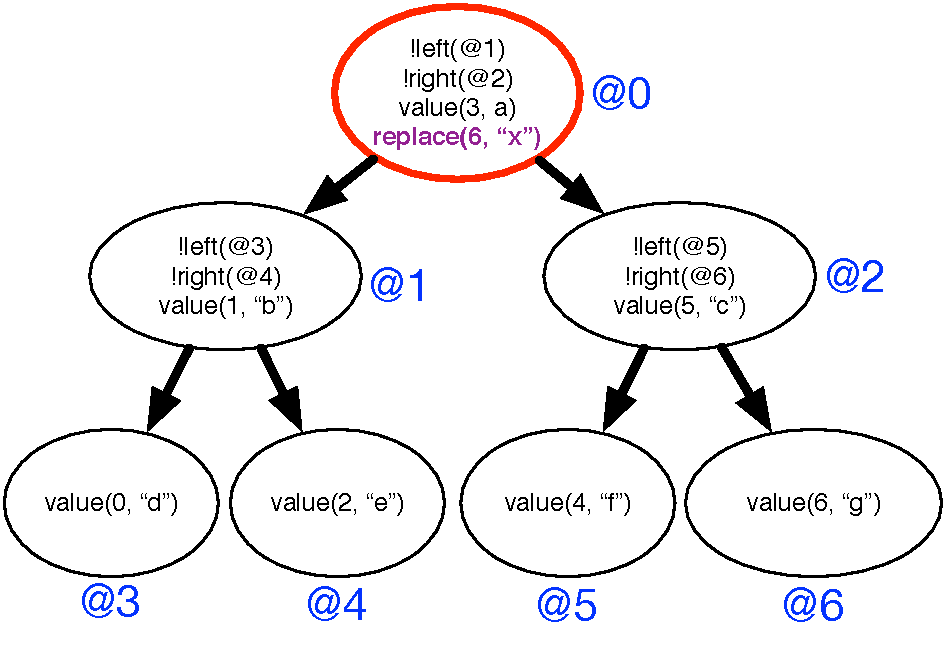
\includegraphics[width=\textwidth]{figures/btree/btree_trace1}
                \caption{Initial database. Replace axiom instantiated at the
                   \texttt{@3} root node.}
                \label{fig:btree_trace1}
        \end{subfigure}%
        ~
        \begin{subfigure}[b]{0.5\textwidth}
                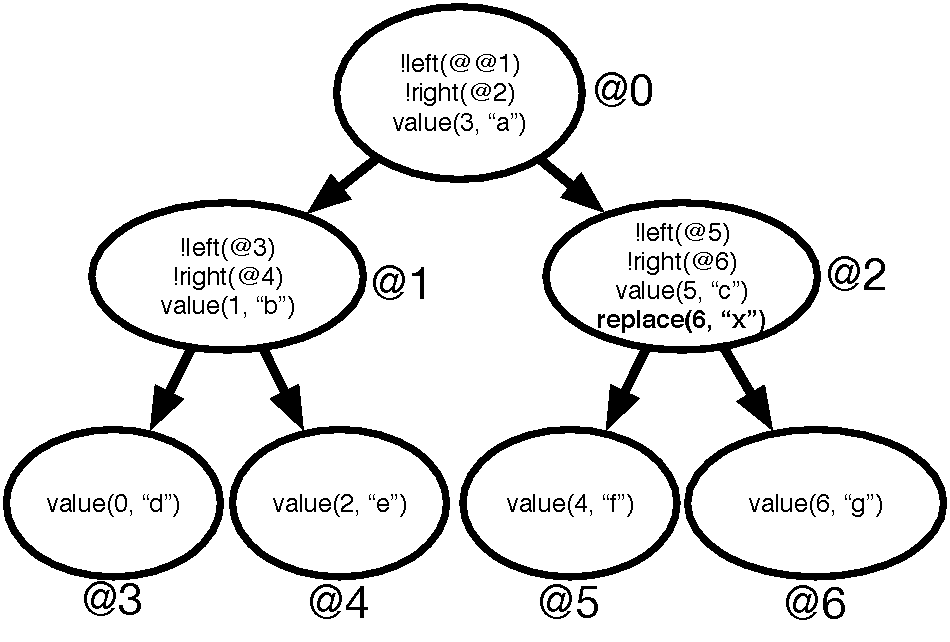
\includegraphics[width=\textwidth]{figures/btree/btree_trace2}
                \caption{After applying rule 3 at node \texttt{@3}. Replace fact
                   sent to node \texttt{@5}.}
                \label{fig:btree_trace2}
        \end{subfigure}\\
        \begin{subfigure}[b]{0.5\textwidth}
                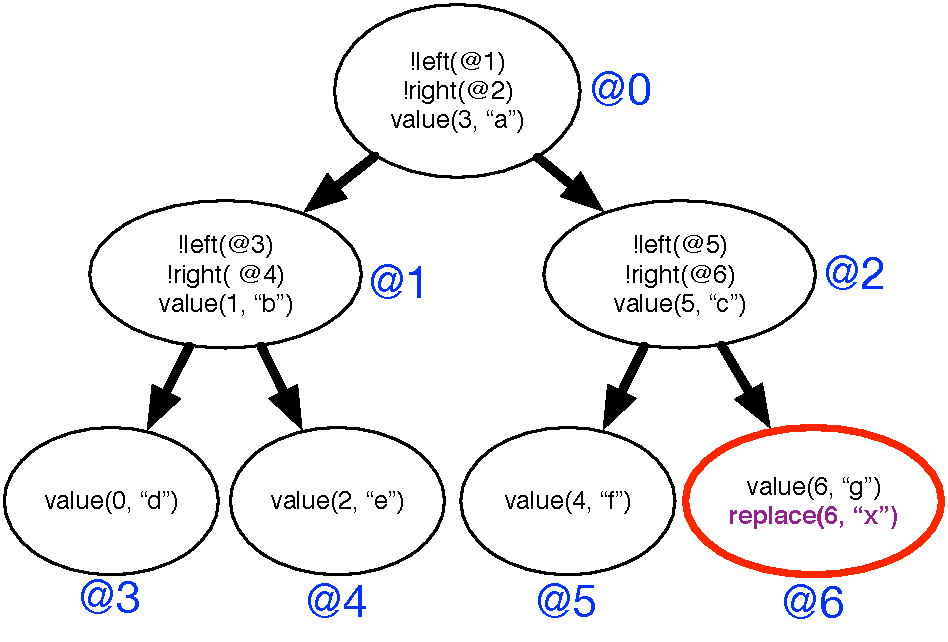
\includegraphics[width=\textwidth]{figures/btree/btree_trace3}
                \caption{After applying rule 3 at node \texttt{@5}. Replace fact
                   reaches node \texttt{@6}.}
                \label{fig:btree_trace3}
        \end{subfigure}%
        ~
        \begin{subfigure}[b]{0.5\textwidth}
                  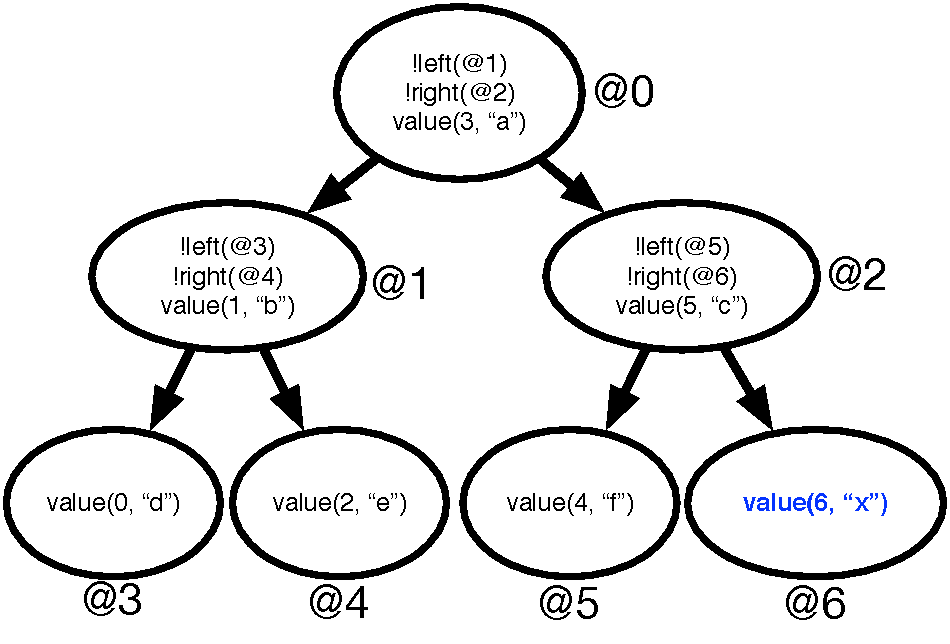
\includegraphics[width=\textwidth]{figures/btree/btree_trace4}
                  \caption{After applying rule 1 at node \texttt{@6}. Value of key 6 has changed to 7.}
                  \label{fig:btree_trace4}
          \end{subfigure}
        \caption{An execution trace for the binary tree dictionary
           algorithm. The first argument of each fact was dropped and the
           address of the node was placed beside it.}\label{fig:btree_trace}
\end{figure}

The present example offers many opportunies for concurrency. If we have multiple
\texttt{replace/3} facts on different nodes, we can perform multiple value
updates at the same time without introducing any kind of database inconsistency.



\subsection{Second Example: Message Routing}

Fig.~\ref{code:message} shows a second LM program, a message routing program
that simulates message transmission through a network of nodes.  Predicate
\texttt{edge/2} represents the connections between nodes, predicate
\texttt{message/3} contains the message content and the route list, and
predicate \texttt{processed/2} keeps count of the number of messages routed at
each node.

\begin{figure}[h!]
\begin{Verbatim}[numbers=left,commandchars=\*\{\},fontsize=\codesize]
type edge(node, node Neighbor).
type linear message(node, string Content, list node Routing).
type linear processed(node, int Total).

!edge(A, B),*label{line:language:message_first1}
message(A, Content, [B | L]),
processed(A, N)
   -o message(B, Content, L),
      processed(A, N + 1).*label{line:language:message_first2}

message(A, Content, []),*label{line:language:message_second1}
processed(A, N)
   -o processed(A, N + 1).*label{line:language:message_second2}

!edge(@1, @2). !edge(@2, @3). !edge(@3, @4). !edge(@1, @3).
processed(@1, 0). processed(@2, 0). processed(@3, 0). processed(@4, 0).
message(@1, "hello world", [@3, @4]).*label{line:language:message_message}
\end{Verbatim}
\caption{Code for routing messages in a graph. There is only one message ("hello
world") to route through nodes \texttt{@3} and \texttt{@4}.}
\label{code:message}
\end{figure}

The first rule
(lines~\ref{line:language:message_first1}-\ref{line:language:message_first2})
grabs the next node in the route list (third argument of \texttt{message/3}) and
ensures that a communication edge exists (through \texttt{edge(A,~B)}). We
increase the number of processed messages by consuming \texttt{processed(A,~N)}
and deriving \texttt{processed(A,~N+1)}.  When the route list is empty, the
message has reached its destination and thus it is consumed (rule in lines
\ref{line:language:message_first1}-\ref{line:language:message_first2}).  Note
that we only need to send one message since there is only one \texttt{message}
axiom (line~\ref{line:language:message_message}).

In Fig.~\ref{fig:message_trace} we present an execution trace of the message
routing program.  The database is represented as a graph structure where the
edges represent the \texttt{edge/2} axioms. In Fig.~\ref{fig:message_trace}~(a)
the database is initialized with the program's axioms.  Note that the initial
\texttt{message/3} fact is instantiated at node \texttt{@1}. After applying rule 1,
we get the database represented in Fig.~\ref{fig:message_trace}~(b), where
the message has been derived at node \texttt{@3}. After applying rule 1
again, the message is then routed to node \texttt{@4}
(Fig.~\ref{fig:message_trace}~(c)) where it will be consumed
(Fig.~\ref{fig:message_trace}~(d)).

\begin{figure}[h]
        \centering
        \begin{subfigure}[b]{0.5\textwidth}
                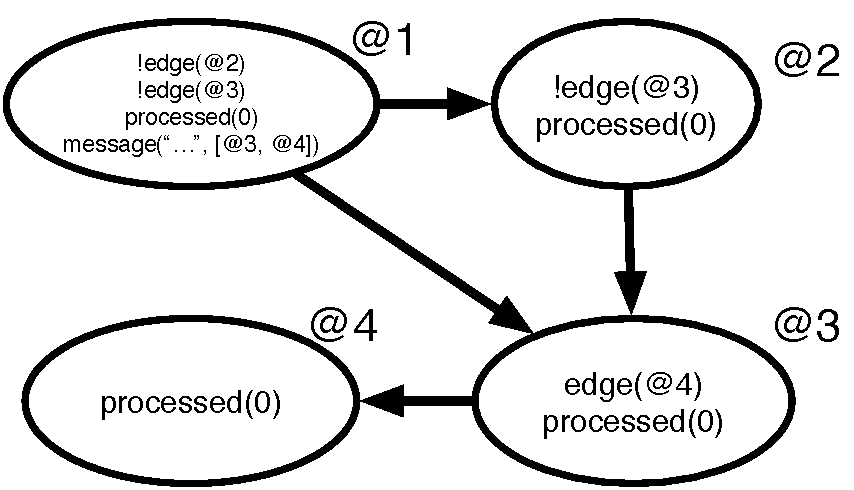
\includegraphics[width=\textwidth]{figures/message/message_trace1}
                \caption{Initial database.}
                \label{fig:message_trace1}
        \end{subfigure}%
        ~
        \begin{subfigure}[b]{0.5\textwidth}
                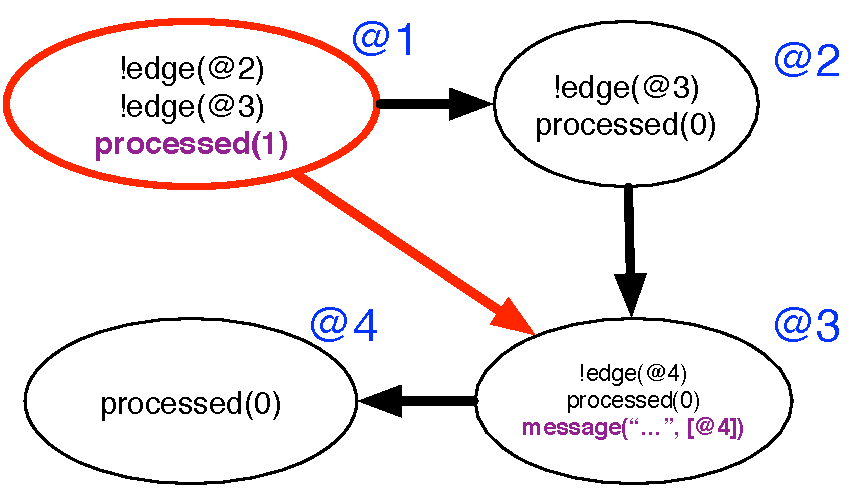
\includegraphics[width=\textwidth]{figures/message/message_trace2}
                \caption{After applying rule 1 at node \texttt{@1}.}
                \label{fig:message_trace2}
        \end{subfigure}\\
        \begin{subfigure}[b]{0.5\textwidth}
                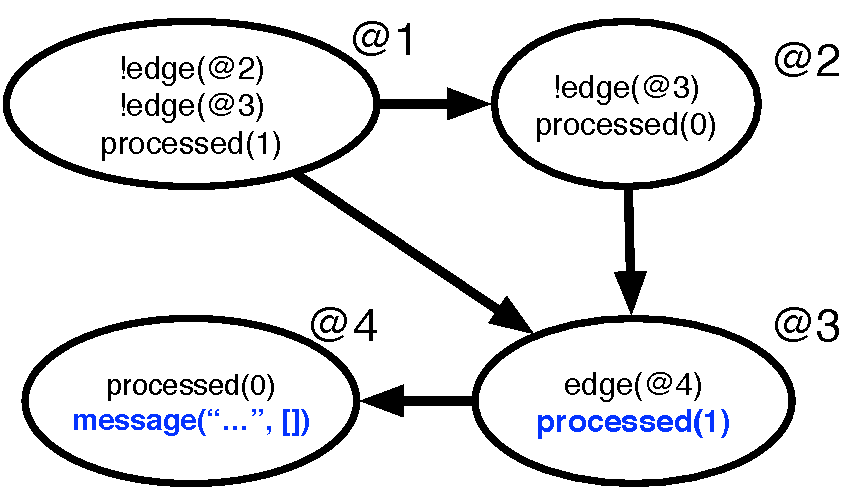
\includegraphics[width=\textwidth]{figures/message/message_trace3}
                \caption{After applying rule 1 at node \texttt{@3}.}
                \label{fig:message_trace3}
        \end{subfigure}%
        ~
        \begin{subfigure}[b]{0.5\textwidth}
                  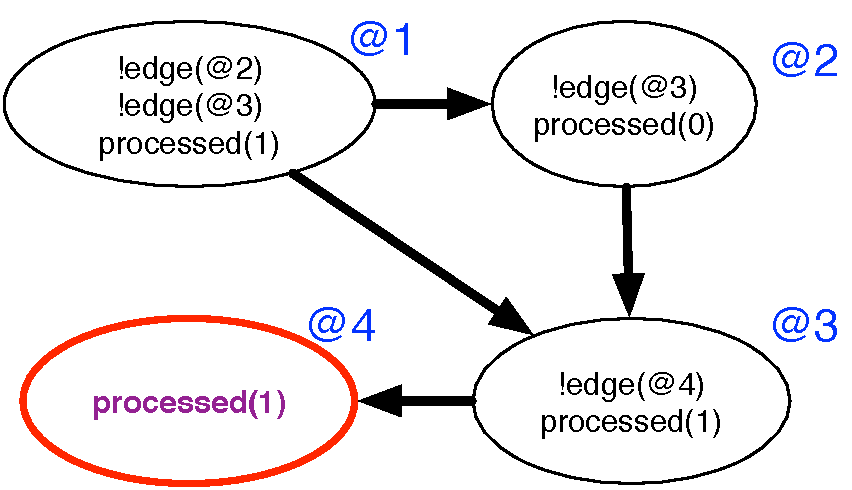
\includegraphics[width=\textwidth]{figures/message/message_trace4}
                  \caption{After applying rule 2 (nodes \texttt{@4}).}
                  \label{fig:message_trace4}
          \end{subfigure}
        \caption{An execution trace for the message program. The message "hello
        world" travels from node \texttt{@1} to node \texttt{@4}.}\label{fig:message_trace}
\end{figure}

\subsection{Third Example: Graph Visit}

\begin{figure}[h!]
\begin{Verbatim}[numbers=left,fontsize=\codesize,commandchars=\*\[\]]
type route edge(node, node).
type linear visit(node).
type linear unvisited(node).
type linear visited(node).

// the program rules*label[line:language:visit_first1]
visit(A), unvisited(A) -o
   visited(A), {B | !edge(A, B) | visit(B)}.*label[line:language:visit_first2]*label[line:language:visit_comprehension]

visit(A), visited(A) -o visited(A).*label[line:language:visit_second]

// axioms: the input data
!edge(@1, @2). !edge(@2, @3). !edge(@1, @4). !edge(@2, @4).
unvisited(@1). unvisited(@2). unvisited(@3). unvisited(@4).

visit(@1).*label[line:language:visit_axiom]
\end{Verbatim}
  \caption{Visit program. Nodes reachable from node \texttt{@1} will be marked
     as \texttt{visited}.}
  \label{code:visit}
\end{figure}
\normalsize

Our final example shown in Fig.~\ref{code:visit} presents another complete LM
program that, for a given graph of nodes, performs a visit to all nodes
reachable from node \texttt{@1}.  The first rule of the program
(lines~\ref{line:language:visit_first1}-\ref{line:language:visit_first2}) visits
node \texttt{A} for the first time: fact \texttt{visited(A)} is derived and a
\emph{comprehension} construct is derived in order to go through all the edge
facts and then derive \texttt{visit(B)} for each neighbor \texttt{B}.  The
second rule (line~\ref{line:language:visit_second}) is fired when the node is
already visited more than once: we keep the \texttt{visited} fact and delete
\texttt{visit/1}. Node \texttt{@1} starts with the \texttt{visit(@1)} fact (line
\ref{line:language:visit_axiom}).

Fig.~\ref{fig:exec_trace} shows a possible execution trace for the visit
program.  After applying the first rule at node \texttt{@1} we get the database
in Fig~\ref{fig:exec_trace}~(b).  Note that node \texttt{@1} is now visited and
nodes \texttt{@2} and \texttt{@4} now have the fact \texttt{visit/1}. At this
point we could either apply rule 1 at node \texttt{@2} or at node \texttt{@4}.
For this specific trace, we apply the rule at node \texttt{@2}, resulting in
Fig.~\ref{fig:exec_trace}~(c). Node \texttt{@4} now has 2 \texttt{visit/1}
facts, thus we can apply rule 1 followed by rule 2, therefore consuming both
\texttt{visit/1} facts and deriving \texttt{visited/1}. In addition, we can also
apply rule 1 at node \texttt{@3} to reach the state of
Fig.~\ref{fig:exec_trace}~(d).

\begin{figure}[h]
        \centering
        \begin{subfigure}[b]{0.5\textwidth}
                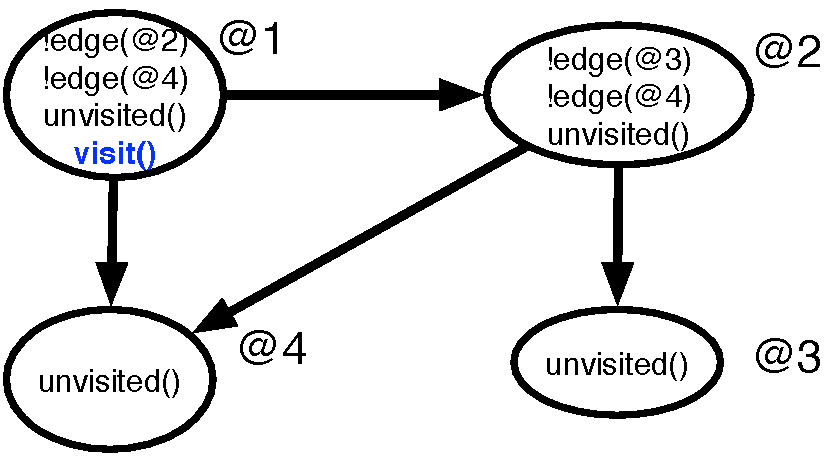
\includegraphics[width=\textwidth]{figures/visit/trace1}
                \caption{Initial database.}
                \label{fig:exec_trace1}
        \end{subfigure}%
        ~ %add desired spacing between images, e. g. ~, \quad, \qquad etc.
          %(or a blank line to force the subfigure onto a new line)
        \begin{subfigure}[b]{0.5\textwidth}
                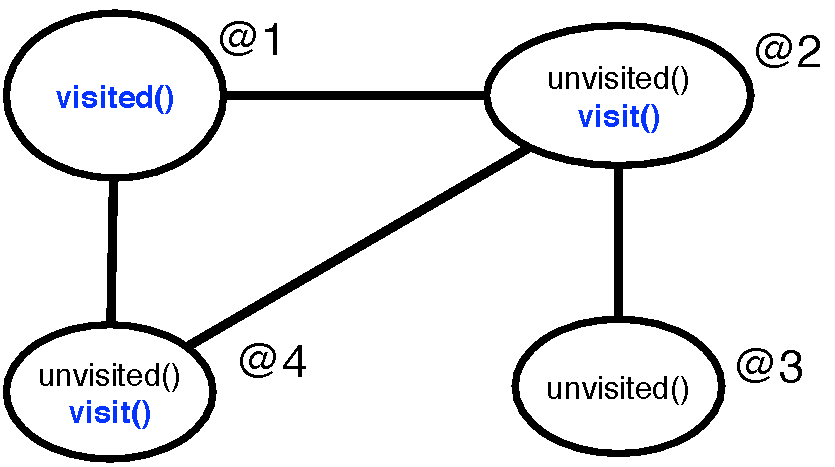
\includegraphics[width=\textwidth]{figures/visit/trace2}
                \caption{After applying rule 1 at node \texttt{@1}.}
                \label{fig:exec_trace2}
        \end{subfigure}\\
        \begin{subfigure}[b]{0.5\textwidth}
                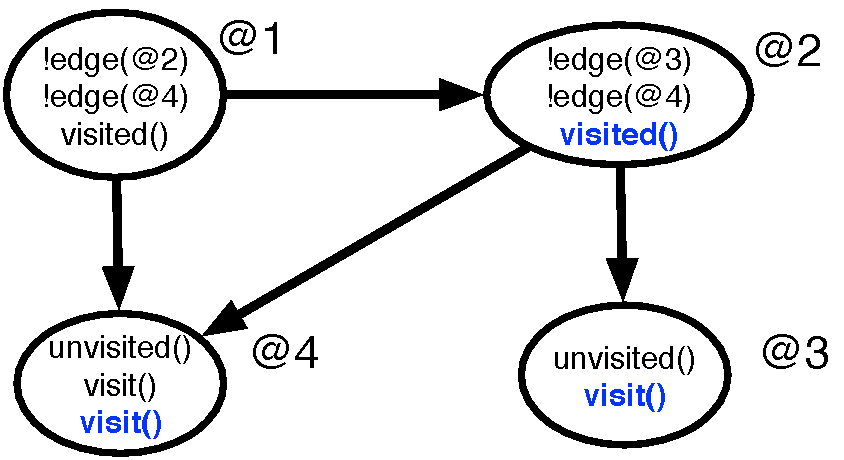
\includegraphics[width=\textwidth]{figures/visit/trace3}
                \caption{After applying rule 1 at node \texttt{@2}.}
                \label{fig:exec_trace3}
        \end{subfigure}%
        ~ %add desired spacing between images, e. g. ~, \quad, \qquad etc.
         %(or a blank line to force the subfigure onto a new line)
        \begin{subfigure}[b]{0.5\textwidth}
                  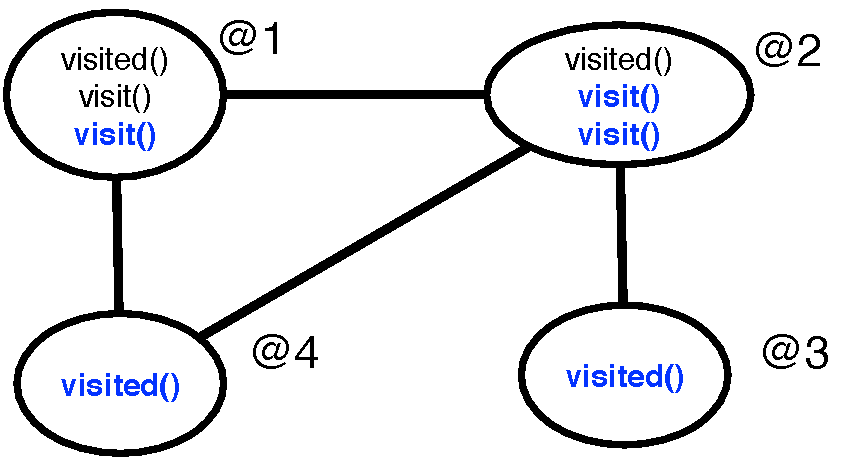
\includegraphics[width=\textwidth]{figures/visit/trace4}
                  \caption{After applying rule 1 and 2 (nodes \texttt{@3},
                        \texttt{@4}).}
                  \label{fig:exec_trace4}
          \end{subfigure}
        \caption{A possible execution trace for the visit program.}\label{fig:exec_trace}
\end{figure}

\subsubsection{Correctness of graph visit}

It is possible to prove that if a graph is connected, then all the nodes will be
become \texttt{visited}, regardless of the order in which we apply the rules.
First, we define what is a visit graph:

\begin{definition}[Visit Graph]
A visit graph is an ordered pair $G = (N, E)$ comprising a set $N$ of nodes together
with a set $E$ of edges. Set $E$ contains pairs $(A, B)$ that correspond to
facts \texttt{\bang edge(A, B)}. For every pair $(A, B) \in E$ there is also a
pair $(B, A) \in E$, representing an undirected edge.
\end{definition}

To prove the correctness property of the program, we first define the main
\emph{invariant} of the program:

\begin{invariant}[Node state]
A node is either \texttt{visited} or \texttt{unvisited}
\end{invariant}
\begin{proof}
Using the axioms we know all nodes start as \texttt{unvisited}.

Rule 1 changes a node from \texttt{unvisited} to \texttt{visited}, while rule 2
keeps the node \texttt{visited}, proving the invariant.
\end{proof}

With this invariant, it is now possible to classify nodes of the graph $G$
according to their state:

\begin{definition}[Node sets] \texttt{visited} nodes are contained in set $V$,
while \texttt{unvisited} nodes are in set $U$. From the node state invariant, we
know that $V \cup U = N$ and $V \cap U = \emptyset$.
\end{definition}

We can now prove an important lemma about sets $V$ and $U$:

\begin{invariant}[Visited set]
Visited set $V$ always increases or stays the same size. The inverse is true for
set $U$.
\end{invariant}
\begin{proof}
Initially, $V = \emptyset$ and $U = N$.

By rule 1, $V$ increases by 1 while $U$ decreases by 1. With rule 2, set
membership remains unchanged.
\end{proof}

In turn, since set membership changes from $U$ to $V$, we now prove the
following:

\begin{lemma}[Edge visits]
The program generates at most one \texttt{visit} per directed edge.
\end{lemma}
\begin{proof}
From the visited set invariant, we know that once nodes become members of set $V$,
they no longer return to set $U$, therefore rule 1 applies once per
node. This rule generates a \texttt{visit} fact per edge.
\end{proof}

In order to prove that all the nodes in the graph are visited, we need to make
sure that the graph is connected.

\begin{definition}[Connected graph]
A connected graph is a graph where every pair of nodes has a path between them.
\end{definition}

Finally, we prove that all nodes will become \texttt{visited}.

\begin{theorem}[Graph visit correctness]
If graph $G$ is connected, set $V$ will eventually include all nodes in $N$,
while $U = \emptyset$.
\end{theorem}
\begin{proof}
Proof by induction.

\begin{itemize}
   \item Base case: axiom \texttt{visit(@1)} adds node \texttt{@1} to $V$. By
   the Edge visits lemma, a \texttt{visit} fact is generate for all edges of
   \texttt{@1}.
   \item Inductive case: assume a set $V'$ and a set $U'$ that contains the
   \texttt{visited} and \texttt{unvisited} nodes, respectively. Since the graph
   is connected, there must be a node $a \in V'$ that is connected to a node $b
   \in U'$. Using the Edge visits lemma, a \texttt{visit(b)} fact is generated,
   swapping $b$ from $U'$ to $V'$.
\end{itemize}

Eventually, set $V$ will include all nodes in $N$.
\end{proof}

\section{LM Syntax}

\begin{table}[h]
\centering
\begin{tabular}{ l l c l }
  Program & $Prog$ & $::=$ & $\Sigma, D$ \\
  List Of Rules & $\Sigma$ & $::=$ & $\cdot \; | \; \Sigma, R$\\
  Database & $D$ & $::=$ & $\Gamma; \Delta$ \\
  Rule & $R$ & $::=$ & $BE \lolli HE \; | \; \forall_{x}. R \; | \; \selector{S}{y}{BE}{HE}$ \\
  Body Expression & $BE$ & $::=$ & $L \; | \; P \; | \; C \; | \; BE, BE \; | \;
\exists_{x}. BE \; | \; \one$\\
  Head Expression & $HE$ & $::=$ & $L \; | \; P \; | \; HE, HE \; | \; EE \; |
  \; CE \; | \; AE \; | \; \one$\\
  
  Linear Fact & $L$ & $::=$ & $l(\hat{x})$\\
  Persistent Fact & $P$ & $::=$ & $\bang p(\hat{x})$\\
  Constraint & $C$ & $::=$ & $c(\hat{x})$ \\
  Selector Operation & $S$ & $::=$ & $\mathtt{min} \; | \; \mathtt{max} \; | \; \mathtt{random}$\\
  
  Exists Expression & $EE$ & $::=$ & $\existsc{\widehat{x}}{SH}$ \\
  Comprehension & $CE$ & $::=$ & $\comprehension{\widehat{x}}{SB}{SH}$ \\

  Aggregate & $AE$ & $::=$ & $\aggregate{A}{y}{\widehat{x}}{SB}{SH_1}{SH_2}$ \\
  Aggregate Operation & $A$ & $::=$ & $\mathtt{min} \; | \; \mathtt{max} \; | \;
\mathtt{sum} \; | \; \mathtt{count} \; | \; \mathtt{collect}$ \\
  
  Sub-Body & $SB$ & $::=$ & $L \; | \; P \; | \; SB, SB \; | \; \exists_{x}. SB$\\
  Sub-Head & $SH$ & $::=$ & $L \; | \; P \; | \; SH, SH \; | \; \one$\\
  
  Known Linear Facts & $\Delta$ & $::=$ & $\cdot \; | \; \Delta, l(\hat{t})$ \\
  Known Persistent Facts & $\Gamma$ & $::=$ & $\cdot \; | \; \Gamma, \bang p(\hat{t})$ \\
\end{tabular}
\caption{Abstract syntax of LM.}\label{tbl:ast}
\end{table}

Table~\ref{tbl:ast} shows the abstract syntax for rules in LM.  A LM program
$Prog$ consists of a list of derivation rules $\Sigma$ and a database $D$.  Each
derivation rule $R$ can be written as $BE \lolli HE$ where $BE$ is the body of a
rule and $HE$ is the head. Rules without bodies are allowed in LM and they are
called \textit{axioms}
(lines~\ref{line:language:dict_axioms1}-\ref{line:language:dict_axioms2} in
Fig.~\ref{code:btree_replace}). Rules without heads are also allowed.

The body of a rule, $BE$, may contain linear ($L$) and persistent ($P$)
\emph{fact expressions} and constraints ($C$). Fact expressions are template
facts that instantiate variables (from facts in the database) such as
\texttt{visit(A)} in line~\ref{line:language:visit_second} in
Fig.~\ref{code:visit}. Variables can be used again in the body for matching and
also in the head when instantiating facts.  Constraints are boolean expressions
that must be true in order for the rule to be fired. Constraints use variables
from fact expressions and are built using a small functional language that
includes mathematical operations, boolean operations, external functions and
literal values.

The head of a rule, $HE$, contains linear ($L$) and persistent ($P$) \emph{fact
templates} which are uninstantiated facts and will derive new facts. The head
can also have \emph{exists expressions} ($EE$), \emph{comprehensions} ($CE$)
and \emph{aggregates} ($AE$). All those expressions may use all the variables
instantiated in the body.

\subsubsection{Graph visit using abstract syntax}\label{visit:ast}

In order to show how programs are represented using the abstract syntax
presented in Table~\ref{tbl:ast}, we present the 2 rules in the graph visit
program shown in Fig.~\ref{code:visit}:

\nopagebreak

\begin{align}
\forall_A. \mathtt{visit}(A), \; \mathtt{unvisited}(A) \lolli & \;
\mathtt{visited}(A), \; \{ B; \; \bang \mathtt{edge}(A, B); \;
\mathtt{visit}(B)\}\\
\forall_A. \mathtt{visit}(A), \; \mathtt{visited}(A) \lolli & \;
\mathtt{visited}(A)
\end{align}

Finally, axioms are represented using an empty body:

\nopagebreak

\begin{align}
\one \lolli & \bang \mathtt{edge}(@1, @2) \\
\one \lolli & \bang \mathtt{edge}(@2, @3) \\
\one \lolli & \bang \mathtt{edge}(@1, @4) \\
\one \lolli & \bang \mathtt{edge}(@2, @4) \\
\one \lolli & \bang \mathtt{unvisited}(@1)  \\
\one \lolli & \bang \mathtt{unvisited}(@2) \\
\one \lolli & \bang \mathtt{unvisited}(@3) \\
\one \lolli & \bang \mathtt{unvisited}(@4) \\
\one \lolli & \bang \mathtt{visit}(@1)
\end{align}

\subsection{Predicates And Facts}

Each fact is an association between a \emph{predicate} and a tuple of values. A
predicate is a pair with a name and a tuple of types (the argument types). LM
rules are type-checked using the predicate declarations in the header of the
program. LM has a simple type system that includes the following simples types:
\emph{node}, \emph{int}, \emph{float}, \emph{string}, \emph{bool}. Recursive
types such as \emph{list X} and \emph{pair X; Y} are also allowed.

\subsection{Selectors}

When a rule body is instantiated using facts from the database, facts are picked
non-deterministically. While our system uses an implementation dependent order
for efficiency reasons, sometimes it is important to sort facts by one of the
arguments because linearity imposes commitment during rule derivation. The
abstract syntax for this construct is $\selector{S}{y}{BE}{HE}$, where $S$ is
the selection operation and $y$ is the variable in the body $BE$ that represents
the value to be selected according to $S$. An example using concrete syntax is
as follows:

\begin{Verbatim}[fontsize=\codesize]
[min => W | !edge(A, B), weight(A, B, W)]
                              -o picked(A, B, W).
\end{Verbatim}

In this case, we will order the \texttt{weight} facts by \texttt{W} in ascending
order and then try to match them. Other operations available are \texttt{max}
and \texttt{random} (to force no pre-defined order at the implementation level).

\subsection{Exists Expression}

Exist constructs ($EE$) are based on the linear logic construct of the same name
and are used to create new node addresses. We can use the new address to
instantiate new facts for the new node.  The following example illustrates the
use of the exists construct, where we derive \texttt{perform-work} at a new node
\texttt{B}.

\begin{Verbatim}[fontsize=\codesize]
   work(A, W) -o exists B. (perform-work(B, W)).
\end{Verbatim}

\subsection{Comprehensions}

Sometimes we need to consume a linear fact and then immediately generate several
facts depending on the contents of the database. To solve this particular need,
we created the concept of comprehensions, which are sub-rules that are applied
with all possible combinations of facts from the database. In a comprehension
$\comprehension{\widehat{x}}{SB}{SH}$, $\widehat{x}$ is a list of variables,
$SB$ is the body of the comprehension and $SH$ is the head.  The body $SB$ is
used to generate all possible combinations for the head $SH$, according to the
facts in the database.  We have already seen an example of comprehensions in the
visit program (Fig.~\ref{code:visit}
line~\ref{line:language:visit_comprehension}). Here, we match \texttt{!edge(A,
B)} using all the combinations available in the database and for each
combination we derive \texttt{visit(B)}.

\subsection{Aggregates}

Another useful feature in logic programs is the ability to reduce several facts
into a single fact.  In LM we have aggregates ($AE$), a special kind of sub-rule
that works very similarly to comprehensions.  In the abstract syntax
$\aggregate{A}{y}{\widehat{x}}{SB}{SH_1}{SH_2}$, $A$ is the aggregate operation,
$\widehat{x}$ is the list of variables introduced in $BE$, $SH_1$ and $SH_2$
and $y$ is the variable in the body $SB$ that represents the values to be
aggregated using $A$. Like comprehensions, we use $\widehat{x}$ to try all
the combinations of $SB$, but, in addition to deriving $SH_1$ for each
combination, we aggregate the values represented by $y$ into a new $y$
variable that is used inside the head $SH_2$.

To better understand aggregates, let's consider a database with the following
facts and a rule:

\begin{Verbatim}[fontsize=\codesize]
price(@1, 3).
price(@1, 4).
price(@1, 5).
count-prices(@1).
count-prices(A) -o [sum => P | . | price(A, P) | 1 | total(A, P)].
\end{Verbatim}

By applying the rule, we consume \texttt{count-prices(@1)} and derive the
aggregate which consumes all the \texttt{price(@1, P)} facts.  These are summed
and \texttt{total(@1,~12)} is derived. LM provides several aggregate operations,
including the \texttt{min} (minimum value), \texttt{max} (maximum value),
\texttt{sum} (add all numbers), \texttt{count} (count combinations) and
\texttt{collect} (collect items into a list).

\section{Operational Semantics}

As said before, the first argument of every predicate must be typed as a
\emph{node}.  For distribution purposes, the body of all derivation rules can
only use facts from the same node in order to avoid concurrency issues.
However, the facts in the head may refer to other nodes, as long as those nodes
are instantiated in the body of the rule.  We drew some inspiration from the
Linda system~\cite{linda} mentioned early on, where the tuple space contains
the data and is used by the processors to communicate and do computation.  This
differs from imperative languages, since in those languages data and computation
are two separate entities.

The execution is performed at the node level and happens non-deterministically
(i.e., any node can be picked to run). This means that the programmer cannot
expect that facts coming from different nodes will be considered as a whole or
partially since the process is non-deterministic. The operational semantics
promises that rule derivations are performed atomically, therefore if a rule
sends many facts to a node then the target node will receive them all at once.
Under these restrictions, computation can then be parallelized by processing
many nodes concurrently.

Each rule in LM has a defined priority that is inferred from its position in the
source file.  Rules at the beginning of the file have higher priority. At the
node level, we consider all the new facts that have been not consider before to
create a priority queue of \emph{candidate rules}.  The queue of candidate rules
is then applied (by priority) and updated as new facts are derived or consumed.
Section~\ref{sec:implementation:rule_engine} gives details in how our
implementation manages the set of candidate rules.

\section{Applications}
In this section, we present solutions to well-known problems. We start with
straightforward graph-based problems such as bipartitness checking and two
versions of the PageRank program. Next, we present the LM version of the
Quick-Sort algorithm, which from a first impression may not fit well under the
programming paradigm offered by LM. Informal correctness and termination proofs
are also included to further show that such important properties are relatively
easy to prove for programs written in LM.

\subsection{Bipartiteness Checking}

The problem of checking if a graph is bipartite can be seen as a 2-color graph
coloring problem.  The code for this algorithm is shown in
Fig.~\ref{language:code:bichecking}. All nodes in the graph start as
\texttt{uncolored}, because they do not have a color yet. The axiom
\texttt{visit(@1, 1)} is instantiated at node \texttt{@1}
(line~\ref{line:language:bc_axiom}) in order to color it with color 1.

If a node is \texttt{uncolored} and needs to be marked with a color \texttt{P}
then the rule in
lines~\ref{line:language:bc_first1}-\ref{line:language:bc_first2} is applied. We
consume the \texttt{uncolored} fact and derive a \texttt{colored(A, P)} to
effectively color the node with \texttt{P}. We also derive \texttt{visit(B,
next(P))} in neighbor nodes to color them with the other color. 

The coloring can fail if a node is already colored with a color \texttt{P} and
needs to be colored with a different color (line~\ref{line:language:bc_third})
or if it has already failed (line~\ref{line:language:bc_fourth}).

\begin{figure}[h!]
\begin{Verbatim}[numbers=left,fontsize=\codesize,commandchars=\*\[\]]
type route edge(node, node).
type linear visit(node, int).
type linear uncolored(node).
type linear colored(node, int).
type linear fail(node).

fun next(int X) : int = if X <> 1 then 1 else 2 end.

visit(@1, 1).*label[line:language:bc_axiom]

visit(A, P), uncolored(A)*label[line:language:bc_first1]
   -o {B | !edge(A, B) | visit(B, next(P))},
      colored(A, P).*label[line:language:bc_first2]

visit(A, P), colored(A, P) -o colored(A, P).*label[line:language:bc_second]
visit(A, P1), colored(A, P2), P1 <> P2 -o fail(A).*label[line:language:bc_third]
visit(A, P), fail(A) -o fail(A).*label[line:language:bc_fourth]
\end{Verbatim}
  \caption{Bipartiteness Checking program.}
  \label{language:code:bichecking}
\end{figure}

\subsubsection{Proof Of Correctness}

In order to show that the code in Fig.~\ref{language:code:bichecking} works as
intended, we first setup some invariants that hold throughout the execution of
the program. Assume that the set of nodes in the graph is represented as $N$.

\begin{invariant}[Node state]
Set of nodes $N$ is partitioned into 4 different states that represent the 4
possible states that a node can be in, namely:

\begin{itemize}
   \item $U$ (\texttt{uncolored} nodes)
   \item $F$ (\texttt{fail} nodes)
   \item $C_{true}$ (\texttt{colored(A, 1)} nodes)
   \item $C_{false}$ (\texttt{colored(A, 2)} nodes)
\end{itemize}
\end{invariant}
\begin{proof}
Initially, all nodes start in set $U$. All the 4 rules of the programs either
keep the node in the same set or exchange the node with another set.
\end{proof}

A bipartite graph is one where in every edge $a \leftrightarrow b$, there is a
valid assignment that makes $a$ member of set $C_{true}$ or $C_{false}$ and node
$b$ member of either $C_{false}$ or $C_{true}$ respectively.

\begin{lemma}[Bipartiteness
   Convergence]\label{language:lemma:bipartite_convergence}
   We now reason from the application of the program rules. After each
   application of an inference rule, one of the following will happen:

   \begin{itemize}
      \item Set $U$ will decrease and set $C_{true}$ or $C_{false}$ will
         increase, with a potential increase in the number of \texttt{visit}
         facts.
      \item Set $C_{true}$ or $C_{false}$ will stay the same, while the number
         of \texttt{visit} facts will be reduced.

      \item Set $C_{true}$ or $C_{false}$ will decrease and set $F$ will
         increase, while the number of \texttt{visit} facts will be reduced.

      \item Set $F$ will stay the same, while the number of \texttt{visit} facts
         decreases.
   \end{itemize}

\end{lemma}
\begin{proof}
Directly from the rules.
\end{proof}

From this invariant, it can be inferred that set $U$ never increases in size
and in a node transition from \texttt{uncolored} to \texttt{colored}, the
database may increase in size. For every other rule application, the database of
facts always decreases. This also means that the program will eventually
terminate, since it is limited by the number of \texttt{visit} facts that can be
generated.

\begin{theorem}[Bipartiteness Correctness]
If the graph is connected and bipartite then the nodes will be partitioned into
sets $C_{true}$ and $C_{false}$, while sets $F$ and $U$ are empty.
\end{theorem}
\begin{proof}
   By induction, we prove that uncolored nodes become part of either $C_{true}$
   and $C_{false}$ and, if there is an edge between nodes in the two sets then
   they have different colors.

   In the base case, we start with empty sets but node \texttt{@1} is made
   member of $C_{true}$. Rule 1 sends \texttt{visit} facts to the neighbors of
   \texttt{@1}, forcing them to be members of $C_{false}$.

   In the inductive case, we have sets $C'_{true}$ and $C'_{false}$ with some
   nodes already colored. From Lemma~\ref{language:lemma:bipartite_convergence},
   we know that $U$ always decreases. Since the graph is bipartite, events 3 and
   4 never happen since there is a possible partitioning of nodes. With event 1,
   we have set $C_{true} = C'_{true}, n$, (or $C_{false}$) where $n$ is the
   node and with event 2, the sets remain the same. Since the graph is
   connected, every node will be colored, therefore event 1 will happen for
   every node of the graph.
\end{proof}

\subsection{PageRank}

PageRank~\cite{Page:2001:MNR} is a well known graph algorithm that is used to
compute the relative relevance of web pages.  The code for a synchronous version
of the algorithm is shown in Fig.~\ref{language:code:pagerank}. As the name
indicates, the pagerank is computed for a certain number of iterations. The
initial pagerank is the same for every page and is initialized in the first rule
(lines
\ref{line:language:spagerank_first1}-\ref{line:language:spagerank_first2}) along
with an accumulator.

The second rule of the program
(lines~\ref{line:language:spagerank_second1}-\ref{line:language:spagerank_second2})
propagates a newly computed pagerank value to all neighbors. The fact
\texttt{neighbor-pagerank} informs the neighbor node about the pagerank value of
node \texttt{A} for iteration \texttt{Iter + 1}. For every iteration, each node
will accumulate the all the \texttt{neighbor-pagerank} facts into the
\texttt{accumulator} fact (lines
\ref{line:language:spagerank_fourth1}-\ref{line:language:spagerank_fourth2}).
When all inbound neighbor pagerank values are accumulated, the third rule
(lines~\ref{line:language:spagerank_third1}-\ref{line:language:spagerank_third2})
is fired and a pagerank value is derived for iteration \texttt{Iter}.

\begin{figure}[h!]
\begin{Verbatim}[numbers=left,fontsize=\codesize,commandchars=\*\[\]]
type outbound(node, node, float).
type linear pagerank(node, float, int).
type numInbound(node, int).
type linear accumulator(node, float Acc, int Left, int Iteration).
type linear neighbor-pagerank(node, node Neighbor, float Rank, int Iteration).
type linear start(node).

const damping = 0.85. // probability of user following a link in the current page.
const iterations = str2int(@arg1). // iterations to compute.
const pages = @world. // number of pages in the graph.

start(A).

start(A), !numInbound(A, T)*label[line:language:spagerank_first1]
   -o accumulator(A, 0.0, T, 1), pagerank(A, 1.0 / float(pages), 0).*label[line:language:spagerank_first2]

pagerank(A, V, Iter), // propagate new pagerank value*label[line:language:spagerank_second1]
Iter < iterations
   -o {B, W | !outbound(A, B, W) | neighbor-pagerank(B, A, V * W, Iter + 1)}.*label[line:language:spagerank_second2]

accumulator(A, Acc, 0, Iter), // new pagerank*label[line:language:spagerank_third1]
!numInbound(A, T),
V = damping + (1.0 - damping) * Acc,
Iter <= iterations
   -o pagerank(A, V, Iter), accumulator(A, 0.0, T, Iter + 1).*label[line:language:spagerank_third2]
	
neighbor-pagerank(A, B, V, Iter), accumulator(A, Acc, T, Iter)*label[line:language:spagerank_fourth1]
   -o accumulator(A, Acc + V, T - 1, Iter).*label[line:language:spagerank_fourth2]
\end{Verbatim}
\caption{Synchronous PageRank program.}
\label{language:code:pagerank}
\end{figure}

\subsubsection{Asynchronous PageRank}

We also have an asynchronous version of the algorithm that trades correctness
with convergence speed since it does not synchronize between iterations.
Figure~\ref{language:code:async_pagerank} shows the LM code for this particular
version, where two major differences can be observed: (1) there is a linear fact
\texttt{neighbor-pagerank} containing the most up-to-date pagerank value of a
neighbor node; (2) a new \texttt{update} fact that forces the node to re-compute
its pagerank by processing the currently available \texttt{neighbor-pagerank}
facts. Rules in
lines~\ref{line:language:apagerank_update1}-\ref{line:language:apagerank_update2}
update the \texttt{neighbor-pagerank} values, while rule in
lines~\ref{line:language:apagerank_new1}-\ref{line:language:apagerank_new2}
asynchronously update the current pagerank value. This last rule derives
multiple \texttt{new-neighbor-rank} that is used to inform the neighbor about
the new pagerank value.

\begin{figure}[h!]
\begin{Verbatim}[numbers=left,fontsize=\codesize,commandchars=\*\#\&]
type outbound(node, node, float).
type linear pagerank(node, float, int).
type numInbound(node, int).
type linear neighbor-pagerank(node, node Neighbor, float Rank, int Iteration).
type linear new-neighbor-rank(node, node Neighbor, float Rank, int Iteration).
type linear update(A).
type linear sum-ranks(node, float).

pagerank(A, 1.0 / float(pages), 0).
update(A).
neighbor-pagerank(A, B, 1.0 / float(pages), 0). // pagerank of B is ...

// save incoming pagerank value.*label#line:language:apagerank_update1&
new-neighbor-rank(A, B, New, Iteration),
neighbor-pagerank(A, B, Old, OldIteration),
Iteration > OldIteration
   -o neighbor-pagerank(A, B, New, Iteration).
new-neighbor-rank(A, B, New, Iteration),
neighbor-pagerank(A, B, Old, OldIteration),
Iteration <= OldIteration
   -o neighbor-pagerank(A, B, Old, OldIteration).*label#line:language:apagerank_update2&

sum-ranks(A, Acc),
NewRank = damping/float(pages) + (1.0 - damping) * Acc,
pagerank(A, OldRank, Iteration)
      -o pagerank(A, NewRank, Iteration + 1),
         {B, W, Delta, Iter | !outbound(A, B, W), Delta = fabs(NewRank -
               OldRank) * W | new-neighbor-rank(B, A, NewRank, Iteration + 1),
               if Delta > bound then update(B) end}.

update(A), update(A) -o update(A).

update(A),*label#line:language:apagerank_new1&
!numInbound(A, T)
   -o [sum => V | B, W, Val, Iter | neighbor-pagerank(A, B, Val, Iter),
         V = Val/float(T) | neighbor-pagerank(A, B, Val, Iter) | sum-ranks(A, V)].*label#line:language:apagerank_new2&
\end{Verbatim}
\caption{Asynchronous PageRank program.}
\label{language:code:async_pagerank}
\end{figure}

\subsubsection{Proof Of Correctness}

To build the proof of correctness, we must again prove several program
invariants. This will help us prove that this partifcular program is similar to
a computation on a nonnegative matrix of of unit spectral radius, which has been
proven that it converges~\cite{DBLP:journals/corr/abs-cs-0606047,
Lubachevsky:1986:CAA:4904.4801}.

\begin{invariant}[Page Invariant]
Each page/node has a single \texttt{pagerank(A, Value, Iteration)} and:
\begin{itemize}
   \item For each outbound link, a single \texttt{\bang outbound(A, B, W)}.
   \item For each inbound link, a single \texttt{neighbor-pagerank(A, B, V, Iter)}.
   \item For each \texttt{\bang outbound(A, B, W)}, a \texttt{neighbor-pagerank(A,
      B, V, Iter}.
\end{itemize}
\end{invariant}

\begin{proof}

All axioms validate the 3 conditions of the variant. Note that the third
condition is also validated by the axioms, although not all axioms are shown in
the code.

In relation to rule application:

\begin{itemize}
   \item Rule 1: inbound link re-derived.
   \item Rule 2: inbound link re-derived.
   \item Rule 3: \texttt{pagerank/2} re-derived.
   \item Rule 4: Nothing happens.
   \item Rule 5: inbound links re-derived in the comprehension.
\end{itemize}
\end{proof}

\begin{lemma}[Neighbor rank lemma]
Given a fact \texttt{neighbor-pagerank(A, B, V, Iter)} and a set of facts
\texttt{new-neighbor-rank(A, B, New, Iter2)}, we end up with a single
\texttt{neighbor-pagerank(A, B, V', Iter')}, where \texttt{Iter} is the greater of
\texttt{Iter} or all of \texttt{Iter2'}.
\end{lemma}
\begin{proof}
By induction on the number of \texttt{new-neighbor-rank} facts.

Base case: \texttt{neighbor-pagerank} remains.

Inductive case: given one \texttt{new-neighbor-rank} fact:

\begin{itemize}
   \item Rule 1: the new iteration is older and thus \texttt{neighbor-pagerank}
   is replaced. By applying induction, we know that we will select either the
   new best iteration or a better iteration from the remaining set of
   \texttt{new-neighbor-rank} facts.
   \item Rule 2: the new iteration is not older and we keep the old
   \texttt{neighbor-pagerank} fact. By induction, we select the best from either
   the current iteration or some other (from the set).
\end{itemize}
\end{proof}

\begin{lemma}[Update lemma]
Given at least 1 \texttt{update/1} fact, rule 7 will run.
\end{lemma}
\begin{proof}
By induction on the number of \texttt{update} facts.

Base case: rule 5 will run.

Inductive case: rule 4 will run first because it has a higher priority, reducing
the number of \texttt{update} facts by one. By induction, we know that by
using the remaining \texttt{update} facts, rule 7 will run.
\end{proof}

\begin{lemma}[Pagerank update lemma]
(1) Given at least one \texttt{update} fact, the \texttt{pagerank(A, $V_{I}$,
I)} fact will be updated to become \texttt{pagerank(A, $V_{I + 1}$, I +
1)}, where \texttt{$V_{I + 1} = damping / P + (1.0 - damping)\sum_{B,
I} (W_{B} \times  N_{I,B})$}.

where $W_B = 1.0/T$ ($T$ from \texttt{\bang numInbound(A, $T$)})
and $N_{I,B}$ from \texttt{neighbor-pagerank(A, B, $N_{I, B}$, $I$)}.

(2) For all \texttt{B} outbound nodes (represented using \texttt{\bang outbound(A, B,
W)}, a \texttt{new-neighbor-rank(B, A, $V_{I+1}$, $I + 1$)} is generated.

(3) For all \texttt{B} outbound nodes (represented using \texttt{\bang outbound(A, B,
W)}), a \texttt{update(B)} is generated if 
$fabs(V_{I + 1} - V_{I}) \times W > bound$.
\end{lemma}
\begin{proof}
Using the Update lemma, rule 5 will necessarily run.

It derives \texttt{sum-ranks(A, $\sum_{B, I} (W_B \times N_{I,B})$)} and
fulfills (3).

\texttt{sum-ranks/2} will necessarily fire rule 6,
computing $V_{I+1}$ and updating \texttt{pagerank}. (2) and (3) are fulfilled
through the comprehension of rule 6.
\end{proof}

\begin{invariant}[New neighbor rank equality]
All \texttt{new-neighbor-rank(A, B, V, I)} facts are generated from a corresponding
\texttt{pagerank(B, V, I)} fact, therefore the iteration of any
\texttt{new-neighbor-rank} is at least the same or less than the iteration of
the current pagerank.
\end{invariant}
\begin{proof}
No axioms to prove.

\begin{itemize}
   \item Rule 3: true, new fact is generated.
   \item Rule 6: the fact is kept.
\end{itemize}
\end{proof}

\begin{invariant}[Neighbor rank equality]
All \texttt{neighbor-pagerank(A, B, V, I)} facts have one corresponding
\texttt{pagerank(B, V, I)} fact and the iteration of the \texttt{neighbor-pagerank}
is the same or less than the current iteration of the corresponding
\texttt{pagerank}.
\end{invariant}
\begin{proof}
By analyzing axioms and rules.

Axioms: true.

Rule cases:

\begin{itemize}
   \item Rule 1: uses \texttt{new-neighbor-rank} fact (use new neighbor rank
         equality invariant).
   \item Rule 2: same fact is re-derived.
\end{itemize}
\end{proof}

\begin{theorem}[Pagerank convergence]
The program will compute the pagerank of all nodes that is within \texttt{bound} error
of an asynchronous pagerank computation.
\end{theorem}
\begin{proof}

Using the program axioms, we start with the same pagerank value for all nodes.
The \texttt{\bang outbound(A, B, W)} fact forms a $n \times n$ square matrix (number
of nodes) and is the so-called "Google Matrix".  All the initial pagerank values
can be seen as a vector that adds up to $1$.

The pagerank computation from the "Pagerank update lemma" computes $V_{I + 1} =
damping / P + (1.0 - damping)\sum_{B, I'} (W_{B} \times N_{I',B})$, where $I' <=
I$
(from Neighbor rank equality invariant).

Consider that each node contains a column $G_i$ of the Google matrix. The
pagerank computation can then be represented as: \newline


$V_{I + 1} = G_i fix([N_{I_1, B_1}, ..., N_{I_p, B_p}])$ \hfill (1) \\


Where $p$ is the number of inbound links and $N_{I_j, B_j}$ is the value of
the \texttt{neighbor-pagerank(A, $B_j$, $N_{I_j, B_j}$, $I_j$)}. The $fix()$
function takes the neighbor vector and expands it with zeros corresponding to
nodes that are not inbound links.

From~\cite{DBLP:journals/corr/abs-cs-0606047, Lubachevsky:1986:CAA:4904.4801} we
know that equation (1) will improve (converge) the pagerank value, given that some new
neighbor pagerank values are sent to node $i$ and by the fact that $G_i$ is a
nonnegative matrix of unit spectral radius. Let's use induction by assuming that there
is at least one \texttt{update/1} fact that
schedules a node to improve its pagerank. We want to prove that such fact will
not only improve the node's pagerank but also the pagerank vector.
If the pagerank vector is now close enough (within \texttt{bound}), then the
program will terminate.

\begin{itemize}
   \item Base case: Since we have an \texttt{update} fact as an axiom, rule 7
   will compute a new pagerank (Pagerank update lemma) for all nodes that is
   improved (from equation (1)). From these updates, a new \texttt{update}
   fact is generated that correspond to nodes that have inbound links from the
   source node and need to update their pagerank. These \texttt{update} facts
   may not be generated if the pagerank vector is close enough to its real
   value.

   \item The induction hypothesis tells us that there is at least one node that
   has an \texttt{update} fact. From pagerank update lemma, this
   generates \texttt{new-neighbor-rank} facts if the new value differs
   significantly from the older value. When this happens and using the ``Neighbor
   rank lemma'', the target node will update its \texttt{neighbor-pagerank} fact
   with the newest iteration and then execute a valid pagerank computation that
   brings the pagerank vector close to its solution.

\end{itemize}

\end{proof}

\subsection{Quick-Sort}

The Quick-Sort algorithm is a divide and conquer sorting algorithm that works by splitting
a list of items into two sublists and then recursively sorting the two sublists.
To split the list, we pick a pivot element and put the items that are smaller than the pivot
into the first sublist and items greater than the pivot into the second list.

The Quick-Sort algorithm is interesting because it does not map immediately to
the graph-based model of LM. Our approach considers that the program starts with
a single node where the initial list is located. Then the list is split as usual
and two nodes are created that will recursively sort the sublists.
Interestingly, this creates a tree that will look similar to a call tree in a
functional programming language.

Fig.~\ref{language:code:quicksort} presents the code for the quick-sort
algorithm in LM. For each sublist to sort, we start with a \texttt{down} fact
that must be (eventually) transformed into an \texttt{up} fact, where the
sublist in the \texttt{up} fact is sorted.  In line~\ref{line:language:qs_axiom}
we start with the initial list at node \texttt{@0}. If the list has a small
number of items, then
lines~\ref{line:language:qs_small1}-\ref{line:language:qs_small2} will
immediately sort it, otherwise the rule in line~\ref{line:language:qs_complex} is applied.  \texttt{split}
first splits the list using the pivot \texttt{Pivot} using rules in
lines~\ref{line:language:qs_split1}-\ref{line:language:qs_split2}.
When there is nothing more to split, the rule in
lines~\ref{line:language:qs_exists1}-\ref{line:language:qs_exists2} uses an
exists construct to create nodes \texttt{B} and \texttt{C}. The sublists are
then sent to nodes \texttt{B} and \texttt{C} using \texttt{down} facts.  Note,
however, that \texttt{back} facts are also derived and are going to be used to
send the sorted list back to the parent using the rule in
line~\ref{line:language:qs_back}.

When the sublists are finally sorted, two \texttt{sorted} facts are derived that
must be matched against \texttt{waitpivot} in the rule in
lines~\ref{line:language:qs_sorted1}-\ref{line:language:qs_sorted2}. The sorted
sublists are appended and then an \texttt{up} fact is finally derived
(line~\ref{line:language:qs_up}).

\begin{figure}[h!]
\begin{Verbatim}[numbers=left,fontsize=\codesize,commandchars=\*\{\}]
type route back(node, node).
type linear down(node, list int).
type linear up(node, list int).
type linear sorted(node, node, list int).
type linear split(node, int list int, list int, list int).
type linear waitpivot(node, int, node, node).
type linear reverse(node, list int, list int, list int).
type linear append(node, list int, list int).

down(@0, tosort).*label{line:language:qs_axiom}

down(A, []) -o up(A, []).*label{line:language:qs_small1}
down(A, [X]) -o up(A, [X]).
down(A, [X, Y]), X < Y -o up(A, [X, Y]).
down(A, [X, Y]), X >= Y -o up(A, [Y, X]).*label{line:language:qs_small2}
down(A, [Pivot | Xs]) -o split(A, Pivot, Xs, [], []).*label{line:language:qs_complex}

split(A, Pivot, [], Smaller, Greater) -o*label{line:language:qs_exists1}
   exists B, C. (back(B, A), back(C, A),
                 down(B, Smaller), down(C, Greater), waitpivot(A, Pivot, B, C)).*label{line:language:qs_exists2}

split(A, Pivot, [X | Xs], Smaller, Greater), X <= Pivot*label{line:language:qs_split1}
   -o split(A, Pivot, Xs, [Y | Smaller], Greater).
split(A, Pivot, [X | Xs], Smaller, Greater), X > Pivot
   -o split(A, Pivot, Xs, Smaller, [Y | Greater]).*label{line:language:qs_split2}
   
waitpivot(A, Pivot, NodeSmaller, NodeGreater),*label{line:language:qs_sorted1}
sorted(A, NodeSmaller, Smaller),
sorted(A, NodeGreater, Greater)
   -o reverse(A, Smaller, [], [Pivot | Greater]).*label{line:language:qs_sorted2}

reverse(A, [X | Xs], S, G) -o reverse(A, Xs, [X | S], G).
reverse(A, [], S, G) -o append(A, S, G).

append(A, [X | Xs], L) -o append(A, Xs, [X | L]).
append(A, [], Result) -o up(A, Result).*label{line:language:qs_up}

up(A, L), back(A, B) -o sorted(B, A, L).*label{line:language:qs_back}
\end{Verbatim}
  \caption{Quick-Sort program written in LM.}
  \label{language:code:quicksort}
\end{figure}

The Quick-Sort program shows that it is possible for applications to manipulate
and change the structure of the graph during run time. This is possible with the
use of the exists operator, which allows the programmer to create new nodes
where facts can be derived. In the case of the Quick-Sort, it allows the program
to create a tree of nodes where sorting can take place concurrently.

\subsubsection{Proof Of Correctness}

The proof of correctness for Quick-Sort will follow a different style than what
we have done up to this point. Instead of proving invariants, we prove what
happens to the database given the presence of some logical facts.

\begin{lemma}[Split lemma]

If fact \texttt{split(A, Pivot, L, Small, Great)} exists then it will be
consumed and \texttt{split(A, Pivot, [], Small' ++ Small, Great' ++ Great)} will
be derived, where elements of \texttt{Small'} are \texttt{<=} \texttt{Pivot} and
elements of \texttt{Great'} are \texttt{> Pivot}.

\end{lemma}
\begin{proof}
By induction on the size of \texttt{L}.
\end{proof}

\begin{lemma}[Reverse lemma]

If fact \texttt{reverse(A, L, R, G)} exists then it will be consumed and
\texttt{reverse(A, [], R' ++ R, G)} will be derived, where \texttt{R'} is the
reverse of \texttt{L}.

\end{lemma}
\begin{proof}
By induction on the size of $L$.
\end{proof}

\begin{lemma}[Append lemma]
If fact \texttt{append(A, L, R)} exists then it will be consumed and
\texttt{append(A, [], R' ++ R)} will be derived, where \texttt{R'} is the reverse of \texttt{L}.
\end{lemma}
\begin{proof}
By induction on the size of $L$.
\end{proof}

\begin{theorem}[Sort theorem]
If fact \texttt{down(A, L)} exists then it will be consumed and a \texttt{up(A,
L')} fact will be derived, where \texttt{L'} is the sorted list.
\end{theorem}
\begin{proof}
By induction on the size of \texttt{L}.

The base cases are proven trivially.

In the inductive case we have:
\begin{Verbatim}[fontsize=\codesize]
down(A, [Pivot | Xs]) -o split(A, Pivot, Xs, [], []).
\end{Verbatim}

We necessarily derive \texttt{split(A, Pivot, Xs, [], [])}. Using the split
lemma we get \texttt{split(A, Pivot, Smaller, Greater)}. With this linear fact
we can only use the rule:

\begin{Verbatim}[fontsize=\codesize]
split(A, Pivot, [], Smaller, Greater) -o
   exists B, C. (back(B, A), back(C, A),
                 down(B, Smaller), down(C, Greater), waitpivot(A, Pivot, B, C)).
\end{Verbatim}

We derive \texttt{back(B, A)}, \texttt{back(C, A)}, \texttt{down(B, Smaller)},
\texttt{down(C, Greater)} and \texttt{waitpivot(A, Pivot, B, C)}. We know that
\texttt{Smaller} and \texttt{Greater} are both smaller (in size) than
\texttt{L}, so, if we use the induction hypothesis, we get \texttt{up(B,
Smaller')} and \texttt{up(C, Greater')}.  These last two facts will be applied
using the following rule:

\begin{Verbatim}[fontsize=\codesize]
up(A, L), back(A, B) -o sorted(B, A, L).
\end{Verbatim}

Generating \texttt{sorted(A, B, Smaller')} and \texttt{sorted(A, C, Greater')}.
Furthermore, we can use the only rule that accepts \texttt{sorted} and
\texttt{waitpivot} facts:

\begin{Verbatim}[fontsize=\codesize]
waitpivot(A, Pivot, NodeSmaller, NodeGreater),
sorted(A, NodeSmaller, Smaller),
sorted(A, NodeGreater, Greater)
   -o reverse(A, Smaller, [], [Pivot | Greater]).
\end{Verbatim}

Returning \texttt{reverse(A, Smaller', [], [Pivot | Greater'])}. By applying the
reverse lemma, we get \texttt{reverse(A, [], Smaller'', [Pivot | Greater'])},
where \texttt{Smaller''} is the reverse of \texttt{Smaller'}.

Now, if we apply the only available rule for \texttt{reverse}, we get
\texttt{append(A, Smaller'', [Pivot | Greater'])}. Applying the append lemma, we
get \texttt{append(A, [], Smaller' ++ [Pivot | Greater'])} and then
\texttt{up(A, Smaller' ++ [Pivot | Greater']).}. We know that \texttt{Smaller'
++ [Pivot | Greater']} is sorted since \texttt{Small'} contains the sorted list
of elements \texttt{<= Pivot} and \texttt{Great'} the elements \texttt{> Pivot}.

\end{proof}



\section{Chapter Summary}

In this chapter we gave an overview of the LM language, including its syntax and
operational semantics.  We also explained how to write programs using all the
facilities provided by LM, including linear facts and comprehensions. We also
explained how to informally prove the correctness of several LM programs.  The implicit
parallelism of LM arising from database partitioning and rule restriction allows
programs to be run in a concurrent fashion.


%\iffalse

\chapter{Local Computation: Rules and Data Structures}

In Chapter~\ref{chapter:language}, we presented different programs that
showcased the declarative core of the LM language. In this chapter, we focus on
the implementation of LM by describing how local computation is achieved, with a
focus on compilation and rule execution.  Next, in
Chapter~\ref{chapter:implementation}, we describe the multithreaded
implementation that allows LM programs to run on multicore architectures. The
coordination aspects of LM, that we introduce later in this dissertation along
with the implementation details, are discussed in depth in
Chapters~\ref{chapter:coordination} and~\ref{chapter:threads}.

This chapter is organized as follows. We start a brief overview of the LM's
implementation, including its compiler and virtual machine. Next, we present the
node data structure, including a detailed description of the data structures
used to efficiently manipulate logical facts.  We also describe how rules are
scheduled locally from newly derived facts stored in the database.  Finally, we
give a description of the compilation algorithm that turns logical rules into
efficient compiled code.


\section{Implementation Overview}
The implementation of LM is composed of a compiler and a virtual machine~(VM).
Figure~\ref{fig:implementation:overview} presents an overview of the compilation
process for LM programs. The two main boxes represent the two major components
of the system, namely, the compiler and virtual machine.

\begin{figure}[ht]
  \centering
  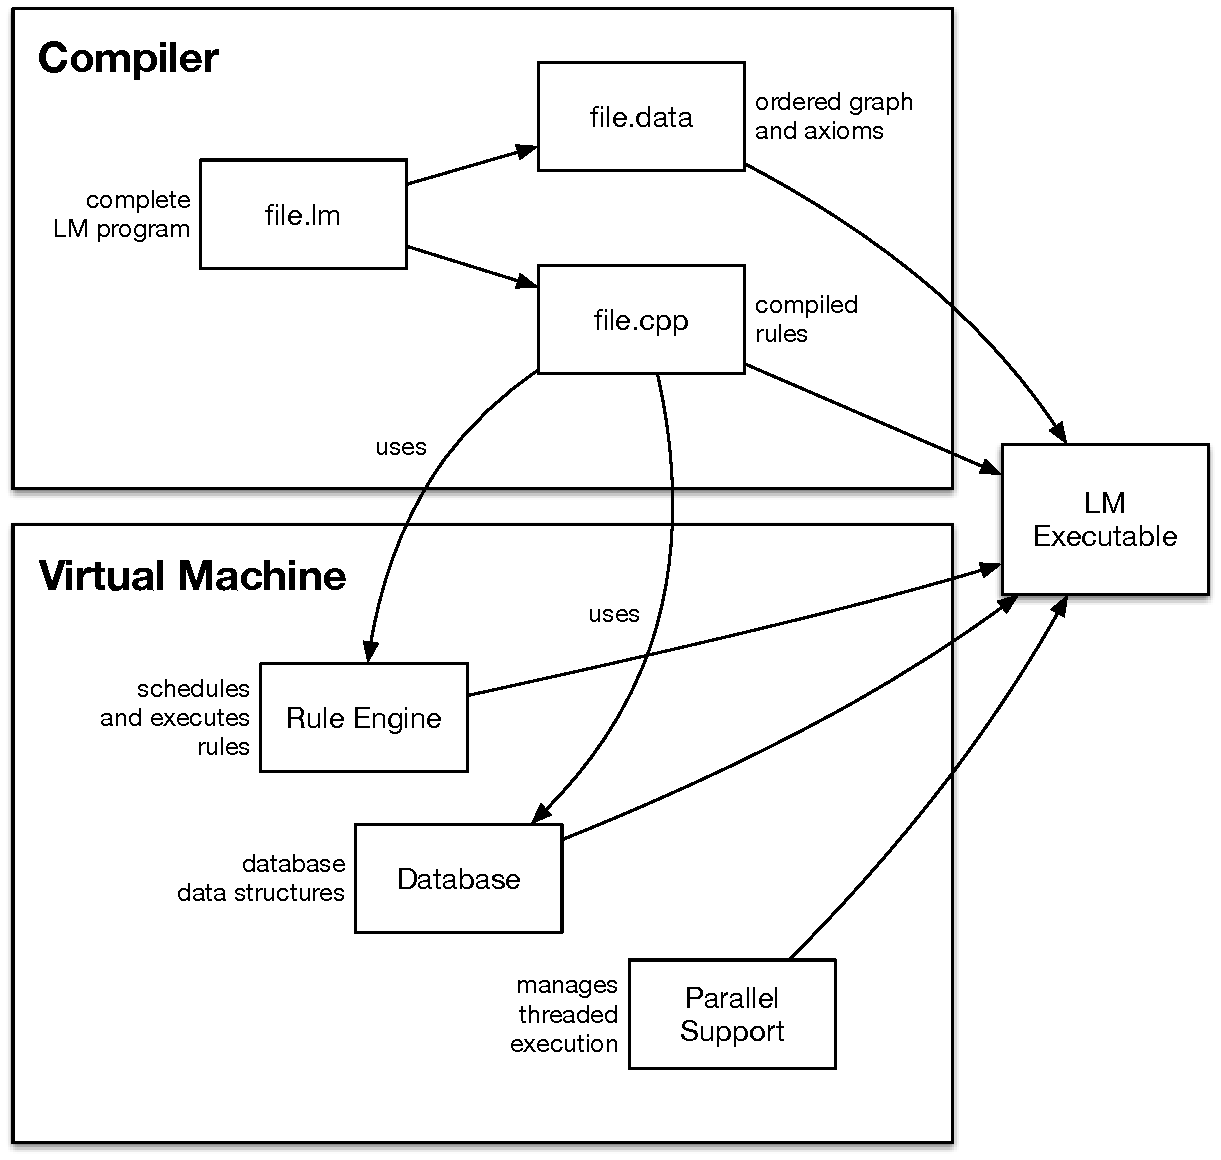
\includegraphics[width=.75\linewidth]{figures/implementation/overview.pdf}
  \caption{Compilation of a LM program into an executable. The compiler
     transforms a LM program into \code{file.cpp}, C++ file with compiled
     rules, and a \code{data} file with the graph structure and initial facts. The virtual
     machine which includes code for managing multithreaded execution and the
     database of facts is then linked with \code{file.cpp} to create a
     standalone executable that can be run in parallel.}
  \label{fig:implementation:overview}
\end{figure}

The virtual machine contains supporting data structures for managing the
database of facts and to schedule the execution of rules. The parallel engine is
also a major part of the virtual machine and is responsible for managing
multithreaded execution by launching threads, managing communication and
and scheduling parallel execution, including coordination.

The compiler transforms LM files into C++ code that use the virtual machine
facilities to implement the program logic.  The compiled code implements the
inference rules of the program and uses the API of the virtual machine to derive
and retract facts and to schedule the execution of rules.  The compiler also
creates a separate file, named \code{file.data}, with the program's initial
facts and graph structure. The graph structure is reconstructed in parallel once
the program starts.

To complete the compilation process, we use a C++ compiler to compile the
virtual machine files and \code{file.cpp} into object files that are then
linked along with \code{file.data}. At the end, we have a standalone
executable that allows the user to input the number of threads to use,
scheduling strategies (i.e., disable coordination), run time measurement
facilities and also database printing facilities.

Alternatively, the programmer may also decide to compile a more general version
of the virtual machine that is able to run byte-code files generated by the
compiler. This allows faster development since the programmer only needs to
recompile the LM program and not the whole stack. However, LM programs will run
slower since the byte-code must be interpreted by the virtual machine. This
severely affects programs with many mathematical operations, especially floating
point computations.

\iffalse
\subsection{Graph Clustering}

The graph structure stored in file \code{file.data} is constructed by the
compiler by analyzing the program's initial facts and then ordering the nodes of
the graph.  In order to distribute computation across threads it is important to
increase locality of communication, so that a node makes most of its
communication to neighbor nodes that are being handled by the same thread. The
graph structure in \code{file.data} is written in order to improve locality and
reduce communication between threads.

The compiler analyzes the node address constants (that are prepended by the
symbol @) and the initial facts of the program. After parsing and type-checking the
program code, the compiler then optimizes the topology by building an internal
representation of the graph.  In this phase, each node address $a$ is mapped
using a function $M(x)$ to a normalized node address $n$. Function $M(x)$ is
bijective and the domain is the set of all nodes described in the source code.
The co-domain of $M$ is the discrete interval $[0, N[$, where $N$ is the number
of nodes in the graph. The byte-code of a LM program includes all the pairs $(x,
M(x))$ so that the runtime system can put this information to use.

We have three methods for defining the function $M(x)$:

\begin{itemize}
   \item \emph{Static}: the compiler uses the node addresses presented in the
      code as long as they fill the discrete interval $[0, N[$.
   \item \emph{Randomized}: the mapping is done randomly.
   \item \emph{Breadth-First}: the mapping is built by picking an arbitrary node, $n_{zero}$
   and setting $M(n_{zero}) = 0$, then we select all neighbors of $n_{zero}$ and start defining
   their mappings in increasing order, $1, \dotsc, N-1$, and adding its neighbors for later processing
   in a breadth first fashion.
\end{itemize}

The breadth-first method is used with the intent of clustering closer nodes in
an ordered fashion.  While not optimal, using a breadth-first approach is very
efficient and has good results for irregular graphs. If we use a static division
of work between $N$ threads, where each thread is responsible to process a
pre-defined set of nodes, we can efficiently slice the codomain of function
$M(x)$ and divide it between the $N$ threads.

For an example, consider the graph in Fig.~\ref{fig:compiler:topology1}. The
node addresses represented are the ones included in the source code. Using a
breadth-first method starting by node 1, we get the following order: 1, 2, 3, 7,
5, 6 and 4. If we had to do a static division with 2 threads, thread 1 would get
1, 2, 3, 7 and thread 2 would get 5, 6 and 4. Note from
Fig.~\ref{fig:compiler:topology1} that only 3 edges exist between the nodes of
thread 1 and thread 2. This greatly reduces communication between threads and
improves parallel efficiency.

\begin{figure}[ht]
  \centering
  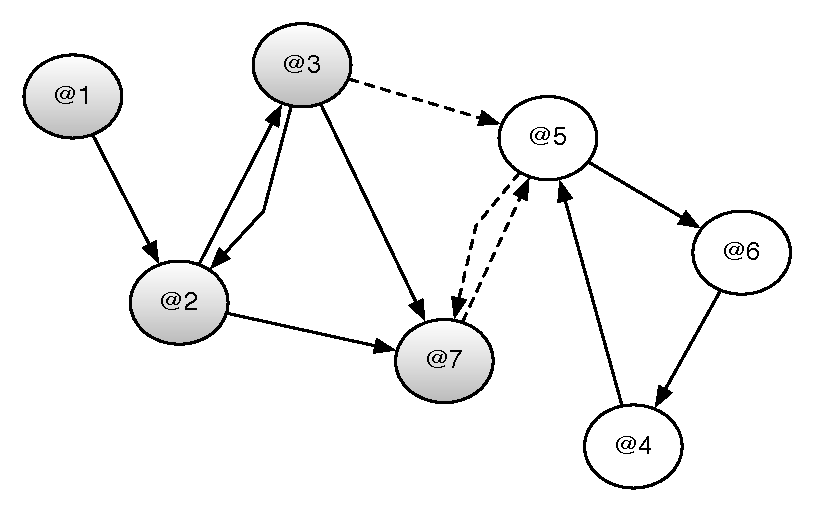
\includegraphics[width=0.6\textwidth]{figures/compiler/topology1.pdf}
  \caption{Topology using a breadth-first method.}
  \label{fig:compiler:topology1}
\end{figure}
\fi


\section{Node Data Structure}\label{sec:data_structures}
The main characteristic of LM rules is that they are constrained by the first
argument\footnote{In the implementation, the first argument of each fact is not
   stored.}. As shown in Fig.~\ref{fig:implementation:vm_overview}, each node
has its own database of linear facts (\emph{Linear DB}) and a database of
persistent facts (\emph{Persistent DB}).  Moreover, since only one thread at a
time will be using a node's database, we do not need to deal with
synchronization issues.

The databases of facts must be implemented efficiently because during matching
of rules we need to restrict the facts using \emph{join constraints}, which fix
arguments of predicates to instantiated values. Each node's database is
implemented using three kinds of data structures:

\begin{itemize}

\item \emph{Trie Data Structures} are used exclusively to store persistent
   facts. Tries are trees where facts are indexed by common prefix arguments.

\item \emph{Doubly Linked List Data Structures} are used to store linear facts.
   We use a double linked list because it is a very efficient way to add and
   remove facts.

\item \emph{Hash Table Data Structures} are used to improve lookup when linked
   lists are too long and when we need to do search filtered by a fixed
   argument. The virtual machine decides which arguments are best to be indexed
   (see Section~\ref{sec:implementation:indexing}) and then uses a hash table
   indexed by the appropriate argument. If we need to go through all the facts,
   we just iterate through all the facts in the table. For collisions, we use
   the doubly linked list data structure mentioned above.

\end{itemize}

Figure~\ref{fig:implementation:hash_table} shows an example for a hash table
data structure for a \texttt{a(int,int)} predicate with 3 linear facts indexed
by the second argument and stored as a doubly linked list in bucket \texttt{2}.
Each linear fact contains the regular list pointers and the fact arguments.
Those are all stored continuously to improve data locality.

\begin{figure}[ht]
\centering
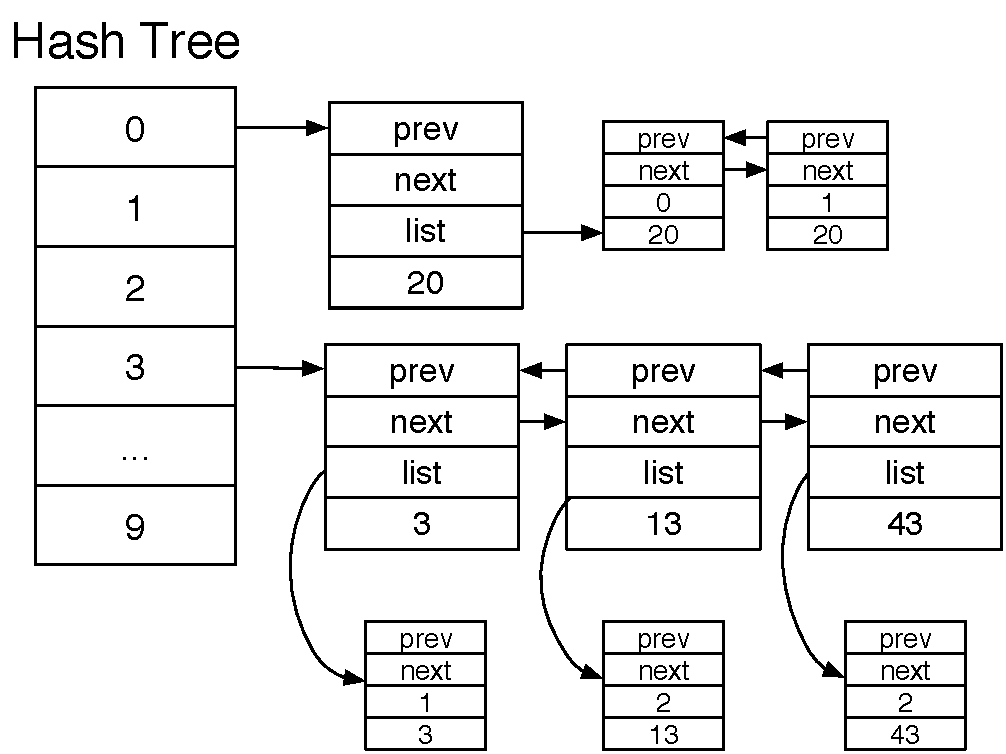
\includegraphics[width=0.6\textwidth]{figures/implementation/hash_table.pdf}
\caption{Hash table and doubly linked data structures for 
   a \texttt{a(int,int)} predicate.}
\label{fig:implementation:hash_table}
\end{figure}

\subsubsection{Locking}

Each node is protected by a main spin-lock that allows threads to change node
attributes. There is also a database spin-lock that protects the internal
database of the node and is locked whenever the node is in the \textbf{working}
state.  

To avoid unnecessary copying, when a node sends facts to a node located in
another thread, the current thread first attempts to lock the database lock of
the target node in order to directly update its database and indexing
structures, otherwise it adds the facts to the list of incoming facts that are
later processed by the owner thread of the target node.


%%%%%%%%%%%%%%%%%%%%%%%%%%%%%%%%%%%%%%%%%%%%%%%%%%%%%%%%%%%%%%%%%%%%%%

\subsection{Rule Engine}
\label{sec:implementation:rule_engine}

The rule engine decides which rules may need to be executed while taking into
account rule priorities. To understand how our engine works, consider the
following set of facts and rules:

\begin{Verbatim}[numbers=left]
a, e(1) -o b.  // rule 1
a -o c.        // rule 2
b -o d.        // rule 3
e(0) -o f.     // rule 4
c -o e(1).     // rule 5

a.
e(0).
\end{Verbatim}

Figure~\ref{fig:implementation:rule_engine} shows the rule engine data
structures for this example. The purpose of each data structure is as follows:

\begin{itemize}

   \item \texttt{Rule Queue} is the bitmap representing the rules scheduled to
      run. The $i^{th}$ is set if the $i^{th}$ rule is scheduled to run;

   \item \texttt{Rule Counter}, which keeps a count of the number of predicates
      needed by the rule that exist in the database. For the rule
      \texttt{a, e(1) -o b} then the rule needs predicates \texttt{a} and
      \texttt{e} and the rule counter is at the most 2 (where the rule can be
      executed).

   \item \texttt{Predicate Bitmap} is a bitmap representing the existence of a
      given predicate in the database;

\end{itemize}

\begin{figure}[t]
   \centering
   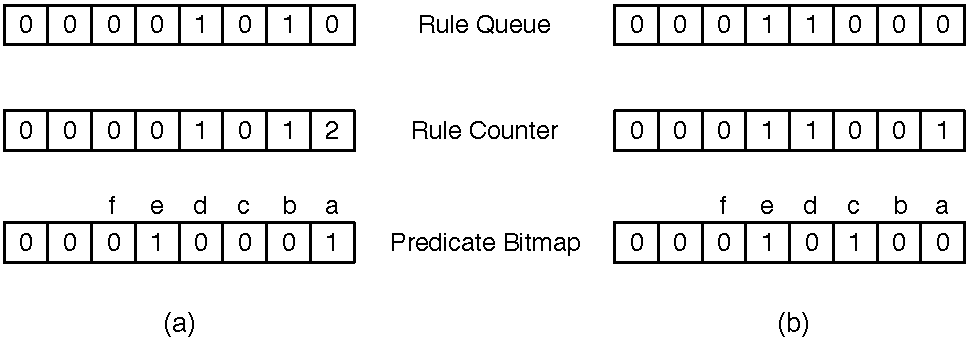
\includegraphics[width=0.8\textwidth]{figures/implementation/rule_queue.pdf}
   \caption{Rule engine data structures (a) before and (b) after applying 
      the rule \texttt{a -o c}.}
   \label{fig:implementation:rule_engine}
\end{figure}

Since we have facts for predicates \texttt{a} and \texttt{e}, the \texttt{Rules
Counter} starts with rules 1, 2 and 4 with 2, 1, 1 predicate counts. Since these
rules have the required counter to be applied, the \texttt{Rule Queue} bitmap
starts with the same three rules.  In order to pick rules for execution, we take
the rule corresponding to the least significant bit from the \texttt{Rule Queue}
bitmap, initially the first rule \texttt{a, e(1) -o b}. However, since we don't
have fact \texttt{e(1)}, this rule fails and its bit in \texttt{Rule Queue} must
be set to 0.  Figure~\ref{fig:implementation:rule_engine}(a) shows the rule
engine data structures at that point.

The next rule in \texttt{Rule Queue} is the second rule \texttt{a -o c}.
Because the this rule will succeed, we must consume fact \texttt{a} and derive
fact \texttt{c}. We thus update \texttt{Predicates Bitmap} accordingly, decrease
the counters for the first and second rule in \texttt{Rule Counter} since such
rules are no longer applicable (\texttt{a} was consumed), and increase the
counter for the fifth rule since \texttt{c} was derived. Finally, to update the
\texttt{Rule Queue}, we must schedule the fifth rule since its counter has been
increased to the required number (we have all predicates).  In the continuation,
the rule engine will schedule the fourth and fifth rules to run.
Figure~\ref{fig:implementation:rule_engine}(b) shows the rule engine data
structures at that point.

Note that every node in the program has the same set of data structures
presented in Fig.~\ref{fig:implementation:rule_engine}. We use 64 bit integers
to implement the 2 bitmaps and an array of 16 bits integers for \texttt{Rule
Counter}.

We do a small optimization to reduce the number of derivations of persistent
facts and, for that, we divide the program rules into two sets: \emph{persistent
rules} and \emph{non persistent rules}. Persistent rules are rules where only
persistent facts are involved. We compile such rules incrementally, i.e., we
attempt to fire all rules where a persistent fact is used. This is called the
\emph{pipelined semi-naive} evaluation and it originated in the P2
system~\cite{Loo-condie-garofalakis-p2}. This evaluation method avoids excessing
re-derivations of the same fact. The order of derivation does not matter for
those rules, since only persistent facts are used.

\subsection{Indexing}\label{sec:implementation:indexing}

To improve fact lookup, the VM employs a fully dynamic mechanism to
decide which argument may be optimal to index.  The algorithm is
performed in the beginning of execution and empirically tries to
assess the argument of each predicate that more equally spreads the
database across the values of the argument.  A single thread performs
the algorithm for all predicates.

The indexing algorithm is performed in three main steps. First, it
gathers lookup statistics by keeping a counter for each
predicate's argument.  Every time a fact search is performed where
arguments are fixed to a value, the counter of such arguments is
incremented. This phase is performed during rule execution for a small
fraction of the nodes in the program.

The second step of the algorithm selects the candidate arguments of each
predicate.  If a predicate was not searched with any fixed arguments, then it
will be not indexed and there are no candidates.  If only one argument was
fixed, then such argument is the only available candidate argument and thus
immediatelly becomes the indexing argument. Otherwise, the top 2 arguments are
selected for the third phase, where \emph{entropy statistics} are collected
dynamically.

During the third phase, each candidate argument has an entropy score.
Before a node is executed, the facts of the target predicate
are used in the following formula applied for the two arguments:

\[
Entropy(A, F) = - \sum_{v \in values(F, A)} \frac{count(F, A = v)}{total(F)} \log_2 \frac{count(F, A = v)}{total(F)}
\]

\noindent where $A$ is the target argument, $F$ is the set of linear facts for
the target predicate, $values(F, A)$ is set of values of the argument $A$,
$count(F, A = v)$ counts the number of linear facts where argument $A$ is equal
to $v$ and $total(F)$ counts the number of linear facts in $F$.  The entropy
value is a good metric because it tells us how much information is needed to
describe an argument. If more information is needed, then that must be the best
argument to index.

For one of the arguments to score, $Entropy(A, F)$ multiplied by the number of
times it has been used for lookup, must be larger than the other argument. The
argument with the best score is selected and then a global variable called
\texttt{indexing\_epoch} is updated. In order to convert the node's linked lists
into hash tables, each node also has a local variable called
\texttt{indexing\_epoch} that is compared to the global variable in order to
rebuild the database according to the new indexing information.

The VM also dynamically resizes the hash table if necessary. When the hash table
becomes too dense, it is doubled in size. When it becomes too sparse, it is
reduced in half or simply transformed back into a doubly linked list. This is
done once in a while, before a node executes.

We have seen very good results with this scheme. The overhead of dynamic
indexing is negligible since programs run almost as fast as if the indices have
been added from the start. However, the programmer can still index predicates
statically, if needed.


\section{Rule Engine}\label{section:local:rule_engine}\label{sec:implementation:rule_engine}
The rule engine decides which rules may need to be executed while taking into
account rule priorities. The rule engine is composed of 3 data structures, which
we describe as follows:

\begin{itemize}

   \item \texttt{Rule Queue} is the bitmap representing the rules scheduled to
      run. The bit $i-1$ is set if the rule number $i$ is scheduled to run,
      which depends on fact availability (do we have all the facts required to
      run the rule?). Rules are executed by fetching the least significant bit
      of the bitmap, unsetting that bit and then executing the corresponding
      rule. This is an operation that is accomplished using the \emph{Bit Scan
      Forward (bsf)} assembly instruction available on x86/x86-64 machines;

   \item \texttt{Rule Counter}, which keeps a count of the number of predicates
      needed by the rule that exist in the database. For the rule \texttt{a,
      e(1) -o b} then the rule needs predicates \texttt{a} and \texttt{e} and
      the rule counter is at the most 2 (where the rule can be executed). The
      \texttt{Rule Queue} bitmap is updated when the rule counter is increments
      or decrements to the maximum possible value;

   \item \texttt{Predicate Bitmap} is a bitmap representing the existence of a
      given predicate in the database. When a predicate becomes available then
      the \texttt{Rule Counter} is updated to take into account the existence of
      new facts.

\end{itemize}

To understand how our engine works, consider the following set of facts and
rules:

\begin{Verbatim}[numbers=left,fontsize=\codesize]
a, e(1) -o b.  // rule 1
a -o c.        // rule 2
b -o d.        // rule 3
e(0) -o f.     // rule 4
c -o e(1).     // rule 5

a.
e(0).
\end{Verbatim}

\begin{figure}[t]
   \centering
   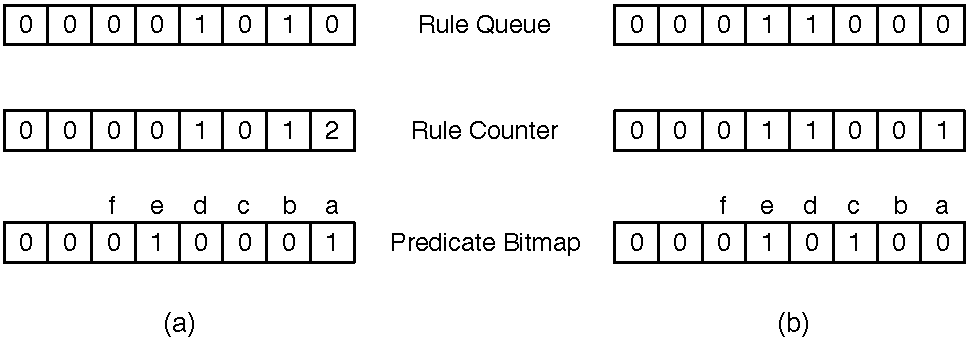
\includegraphics[width=0.8\textwidth]{figures/implementation/rule_queue.pdf}

   \caption{Rule engine data structures for a program with five rules. The
      initial state is represented in (a), where the rules scheduled to run are
      1, 2 and 4. After attempting rule 1, bit 0 is unset from the \emph{Rule
      Queue}, resulting in (b). Figure (c) is the result of deriving rule 2,
      \code{a -o c}, which marks rule 5 in the \emph{Rule Queue} since the rule
      is now marked as ``available`` in the \emph{Rule Counter}.}

   \label{fig:implementation:rule_engine}
\end{figure}

Figure~\ref{fig:implementation:rule_engine} shows the rule engine data
structures for this example. Since we have facts for predicates \texttt{a} and
\texttt{e}, the \texttt{Rules Counter} starts with rules 1, 2 and 4 with 2, 1, 1
predicate counts. Since these rules have the required counter to be applied, the
\texttt{Rule Queue} bitmap starts with the same three rules
(Fig.~\ref{fig:implementation:rule_engine}(a)). In order to pick rules for
execution, we take the rule corresponding to the least significant bit from the
\texttt{Rule Queue} bitmap, initially the first rule \texttt{a, e(1) -o b}.
However, since we don't have fact \texttt{e(1)}, this rule fails and its bit in
\texttt{Rule Queue} must be set to 0.
Figure~\ref{fig:implementation:rule_engine}(b) shows the rule engine data
structures at that point.

The next rule in \texttt{Rule Queue} is the second rule \texttt{a -o c}.
Because the this rule succeeds, fact \texttt{a} is consumed and fact \texttt{c}
is derived. We thus update \texttt{Predicates Bitmap} accordingly, decreasing
the counters for the first and second rules in \texttt{Rule Counter} since such
rules are no longer applicable (\texttt{a} was consumed), and increase the
counter for the fifth rule since \texttt{c} was derived. Finally, to update the
\texttt{Rule Queue}, we must schedule the fifth rule since its counter has been
increased to the required number (we have all predicates).  In the continuation,
the rule engine will schedule the fourth and fifth rules to run.
Figure~\ref{fig:implementation:rule_engine}(b) shows the rule engine data
structures at that point.

Note that every node in the program has the same set of data structures
presented in Fig.~\ref{fig:implementation:rule_engine}. We use 64 bit integers
to implement the 2 bitmaps and an array of 16 bits integers for \texttt{Rule
Counter}.

We do a small optimization to reduce the number of derivations of persistent
facts and, for that, we divide the program rules into two sets: \emph{persistent
rules} and \emph{non persistent rules}. Persistent rules are rules where only
persistent facts are involved. We compile such rules incrementally, i.e., we
attempt to fire all rules where a persistent fact is used. This is called the
\emph{pipelined semi-naive} evaluation and it originated in the P2
system~\cite{Loo-condie-garofalakis-p2}. This evaluation method avoids excessive
re-derivations of the same fact. The order of derivation does not matter for
those rules, since only persistent facts are used.



\section{Compilation}
As an intermediate step, our compiler first transforms rules into high level
instructions that are then transformed into C++. In Appendix~\ref{appendix:vm}
we present an overview of the high level instructions that can be used as a
reference to the operations that are required by the compiler. In this section,
we present the main algorithm of the compiler and its key optimizations. To make
our presentation more readable, we present our examples using pseudo-code
instead of C++ code.

\subsection{Ordinary Rules}\label{sec:compile}

After a rule is compiled, it must respect the \emph{fact constraints}
(facts must exist in the database) and the \emph{join constraints} that can be
represented by variable constraints and/or boolean expressions. For instance,
consider the second rule of the bipartiteness checking program presented in
Fig.~\ref{language:code:bichecking}:

\begin{Code}
visit(A, P),
colored(A, P)
   -o colored(A, P).
\end{Code}

The fact constraint include the facts required to trigger the rule, namely
\code{visit(A, P)} and \code{colored(A, P)}, and the join constraints include
the implicit constraint that the second argument of \code{visit} must be equal
to the second argument of \code{colored} because the variable \code{P} is used
for both arguments. However, rules may also have explicit constraints, such as:

\begin{Code}
visit(A, P1),
colored(A, P2),
P1 <> P2
   -o fail(A).
\end{Code}

The data structures presented in Section~\ref{sec:data_structures} support
iteration over facts and for linear facts, they also support deletion. Iteration
is provided through \emph{iterators}. For linked lists, the iterator points to
the linear fact in the list and uses the \code{next} field to traverse the list.
For hash tables, it is possible to iterate through the whole table or iterate
through a single bucket. For tries, while iteration goes through every fact, the
operation can be customized with join constraints in order to prune search. To
illustrate how rules are compiled, consider again the rule:

\begin{Code}
visit(A, P),
colored(A, P)
   -o colored(A, P).
\end{Code}

The compiler transforms the rule into two nested \emph{while} loops, as follows:

\begin{LineCode}
colored_list <- linked_list("colored")
visit_list <- linked_list("visit")
visit <- visit_list.head()
while(visit is valid)
{
   colored <- colored_list.head() // Retrieve first element of the list.
   while(colored is valid)
   {
      if(visit.get_int(1) == colored.get_int(1)) { // Equal arguments?
         // New fact is derived.
         new_colored <- create_fact("colored") // New fact for predicate colored.
         new_colored.set_int(1, visit.get_int(1)) // Set arguments.

         colored_list.add(new_colored) // Add new fact to the linked list.

         // Deleting used up facts.
         colored <- colored_list.delete_and_next(colored)
         visit <- visit_list.delete_and_next(visit)
         goto next
      }
      colored <- colored.next()
   }
   visit <- visit.next()
next:
   continue
}
\end{LineCode}

The compilation algorithm iterates through the atomic propositions of the rule's
LHS and creates nested loops to try all the possible combinations of facts.  For
this rule, all the pairs of facts \code{colored} and \code{visit} must be
searched until the implicit constraint is true. First, the \code{visit} linked
list is iterated over by first retrieving the head fact and then using the
\code{next} pointer of each fact. Inside this outer loop, a nested \code{while}
loop is created for predicate \code{colored}. This inner loop includes a check
for the constraint.

If the constraint expression is true then the rule matches and a new
\code{colored} fact is derived and two used linear facts are consumed by
deleting them from the linked lists. After the rule is derived, the \code{visit}
and \code{colored} facts are deleted from the linked list and the pointers
adjusted to the next elements of each list. Afterwards, the \code{goto next}
statement is used to jump to the outer loop, which will use the new fact
pointers. This forces the procedure to try all the combinations of the rule from
the database.  Furthermore, we must jump to the first linear loop because we
cannot use the next fact from the deepest loop since we may have constraints
between the first linear loop and the deepest loop that were validated using
deleted facts.

If the implicit constraint failed, another \code{colored} fact would be checked
by assigning \code{colored} to \code{colored.next()}.  Likewise, if the initial
\code{visit} fact fails for all \code{colored} facts, then the next
\code{visit} fact in the list is tried by following the \code{next} pointer.

In order to understand how rule priorities affect compilation, consider a
slightly different bipartiteness checking program where the second and third
rules are swapped:

\begin{LineCode}[commandchars=\*\[\]]
visit(A, P),
uncolored(A)
   -o {B | !edge(A, B) -o visit(B, next(P))},
      colored(A, P).

visit(A, P1),
colored(A, P2),
P1 <> P2
   -o fail(A).*label[line:implementation:higher]

*textbf[visit(A, P),]
*textbf[colored(A, P)]
   *textbf[-o colored(A, P).]

visit(A, P),
fail(A)
   -o fail(A).
\end{LineCode}

The procedure for the rule being compiled cannot be the same since the derived
\code{colored} fact is used in the LHS of a higher priority rule, namely, the
rule in line~\ref{line:implementation:higher}. Once the \code{colored} fact is
derived, the procedure must return to schedule the higher priority rule, as
follows:

\begin{LineCode}[commandchars=\$\#\&]
colored_list <- linked_list("colored")
visit_list <- linked_list("visit")
colored <- colored_list.head()
while(colored is valid)
{
   visit <- visit_list.head() // Retrieve first element of the list.
   while(visit is valid)
   {
      if(visit.get_int(1) == colored.get_int(1)) { // Equal arguments?
         new_colored <- create_fact("colored") // New fact for predicate colored.
         new_colored.set_int(1, visit.get_int(1)) // Set arguments.

         // New fact is derived.
         colored_list.add(new_colored) // Add new fact to the linked list.

         // Deleting facts.
         colored_list.delete_and_next(colored)
         visit_list.delete_and_next(visit)
         $textbf#return&
      }
      visit <- visit.next()
   }
   colored <- colored.next()
}
\end{LineCode}

This enforces the priority semantics of the language described in
Section~\ref{sec:language:semantics}. When a rule derives facts
that were used as input to a higher priority rule, the initial rule is only
derived once because the newly derived facts may trigger the derivation of a
higher priority rule.
    
\begin{figure}
\begin{algorithm}[H]
 \KwData{Rule R1, Rules}
 \KwResult{Compiled Code}
 $LHSProps \longleftarrow LHSAtomicPropositionsFromRule(R1)$\;
 $Constraints \longleftarrow ConstraintsFromRule(R1)$\;
 $Code \longleftarrow CreateFunctionForRule()$\;
 $FactIterators \longleftarrow []$\;
 $CompiledProps = []$\;
 \While{$LHSProps$ not empty}{
  $Prop \longleftarrow RemoveBestProposition(LHSProps)$\;
  $CompiledProps.push(Prop)$\;
  $Iterator \longleftarrow Code.InsertIteration(Prop)$\;
  $FactIterators.push(Iterator)$\;
  \tcp{Select constraints that are covered by CompiledFacts.}
  $NextConstraints \longleftarrow RemoveConstraints(Constraints, CompiledProps)$\;
  $Code.InsertConstraints(NextConstraints)$\;
 }
 $RHSProps = RHSAtomicPropositionsFromRule(R1)$\;
 \While{$RHSProps$ not empty}{
    $Prop \longleftarrow RemoveFact(RHSProps)$\;
    $Code.InsertDerivation(Prop)$\;
 }
 \For{$Iterator \in FactIterators$}{
    \If{$IsLinear(Iterator)$}{
       $Code.InsertRemove(Iterator)$\;
    }
 }
 \tcp{Enforce rule priorities.}
 \uIf{$FactsDerivedUsedBefore(Rules, R1)$}{
    $Code.InsertReturn()$\;
 }
 \Else{
    $Code.InsertGoto(FirstLinear(FactIterators))$\;
 }
 \Return{$Code$}
\end{algorithm}
 \mycap{Compiling LM rules into C++ code.}
 \label{alg:compile_rule}
\end{figure}

Figure~\ref{alg:compile_rule} presents the algorithm for compiling rules into
C++ code. First, we split the rule's RHS into atomic propositions and
constraints. Fact expressions map directly to iterators while fact constraints
map to \emph{if} expressions. A possible compilation strategy is to first
compile all the atomic propositions and then compile the constraints. However,
this may require unneeded database lookups since some constraints may fail
early.  Therefore, our compiler introduces constraints as soon as all the
variables in the constraint are all included in the already compiled atomic
propositions. The order in which fact propositions are selected for compilation
does not interfere with the correctness of the compiled code, thus our compiler
selects the atomic proposition ($RemoveBestProposition$) that needs the highest
number of join constraints, in order to prune search and avoid undesirable
database lookups. If two atomic propositions have the same number of new
constraints, then the compiler always picks the persistent proposition since
persistent facts are not deleted.

Derivation of new facts belonging to the local node requires only that the new
facts are added to the local node data structure. Facts that belong to other
nodes are sent using an appropriate runtime API.

\subsection{Persistence Checking}

Not all linear facts need to be deleted. For instance, in the compiled rule
above, the fact \code{colored(A, P)} is re-derived in the rule's RHS.  Our
compiler is able to turn linear loops into persistent loops for linear facts
that are consumed and then asserted. The rule is then compiled as follows:

\begin{LineCode}[commandchars=\$\#\&]
colored_list <- linked_list("colored")
visit_list <- linked_list("visit")
colored <- colored_list.head()
while(colored is valid)
{
   visit <- visit_list.head() // Retrieve first element of the list.
   while(visit is valid)
   {
      if(visit.get_int(1) == colored.get_int(1)) { // Equal arguments?
         // Delete visit.
         visit <- visit_list.delete_and_next(visit) // Get next visit fact.
         goto next$label#line:implementation:goto&
      }
      visit <- visit.next()
$textbf#next:&
      $textbf#continue&
   }
   colored <- colored.next()
}
\end{LineCode}

In this new version of the code, only the \code{visit} facts are deleted, while
the \code{colored} facts remain untouched. In the bipartiteness checking
program, each node has one \code{colored} fact and this compiled code simply
filters out the \code{visit} facts with the same color. Please note that the
\code{colored} facts are now iterated in the outer loop in order to make the
\code{goto} statement jump to the inner loop. This is now possible because the
\code{colored} fact is not deleted during rule derivation.

\subsection{Updating Facts}

Many inference rules consume and then derive the same predicate but with
different arguments. The compiler recognizes those cases and, instead of
consuming the fact from its linked list or hash table, it updates the fact
in-place. As an example, consider the following rule:

\begin{Code}
new-neighbor-pagerank(A, B, New),
neighbor-pagerank(A, B, Old)
   -o neighbor-pagerank(A, B, New).
\end{Code}

Assuming that \code{neighbor-pagerank} is stored in a hash table and indexed by
the second argument, the code for the rule above is as follows:

\begin{LineCode}
new_neighbor_pagerank_list <- linked_list("new-neighbor-pagerank")
neighbor_pagerank_table <- hash_table("neighbor-pagerank")
new_neighbor_pagerank <- new_neighbor_pagerank.head()
while(new_neighbor_pagerank is valid)
{
   // Hash table for neighbor-pagerank is indexed by the second argument,
   // therefore we search for the bucket using the second argument
   // of new-neighbor-pagerank.
   neighbor_pagerank <- neighbor_pagerank_table.lookup(new_neighbor_pagerank.get_node(1))
   while(neighbor_pagerank is valid)
   {
      if(new_neighbor_pagerank.get_node(1) == neighbor_pagerank.get_node(1))
      {
         // Update fact argument.
         neighbor_pagerank.set_float(2, new_neighbor_pagerank.get_float(2))
         new_neighbor_pagerank <- new_neighbor_pagerank_list.
                  delete_and_next(new_neighbor_pagerank)
         goto next
      }
      neighbor_pagerank <- neighbor_pagerank.next()
   }
   new_neighbor_pagerank <- new_neighbor_pagerank.next()
next:
   continue
}
\end{LineCode}

Note that \code{neighbor-pagerank} fact is updated using \code{set\_float}. The
rule also does not return since it is the highest priority rule. If there was a
higher priority rule using \code{neighbor-pagerank}, then the code would have to
return since the act of updating a fact is equivalent to deriving a new one.

\subsection{Enforcing Linearity}

We have already introduced the \code{goto} statement as a mechanism to avoid
reusing deleted linear facts. However, this is not enough in order to enforce
linearity of facts. Consider the following inference rule:

\begin{Code}
add(A, N1),
add(A, N2)
   -o add(A, N1 + N2).
\end{Code}

Using the standard compilation algorithm, two nested loops are created, one for
each \code{add} fact. However, notice that there is an implicit constraint (the
two \code{add} linear facts must be different) when creating the iterator for
\code{add(A, N2)} since this fact cannot be the same as the first one. That
would invalidate linearity since a single linear fact would be used to prove two
linear facts. This is easily solved by adding a constraint in the inner loop by
checking if the second fact is the same as the first one.

\begin{LineCode}
add_list <- linked_list("add")
add1 <- add_list.head()
while(add1 is valid)
{
   add2 <- add_list.head()
   while(add2 is valid)
   {
      if(add1 != add2)
      {
         add1.set_int(1, add1.get_int(1) + add2.get_int(1))
         add2 <- add_list.delete_and_next(add2)
         goto next
      }
      add2 <- add2.next()
   }
   add1 <- add1.next()
next:
   continue
}
\end{LineCode}

Figure~\ref{fig:local:update_add} presents the steps for executing this rule
when the database contains three facts. The fact variables never point to the
same fact.

\begin{figure}
\centering
\begin{minipage}{.5\textwidth}
  \centering
  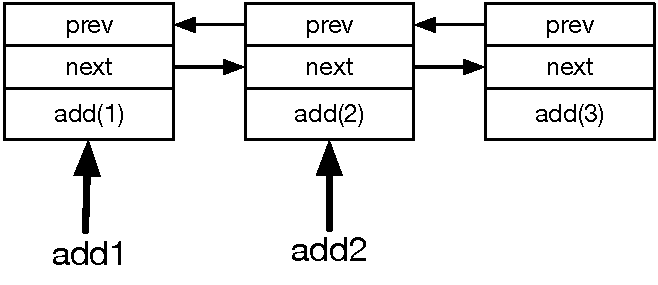
\includegraphics[width=.8\linewidth]{figures/compiler/update}
\end{minipage}%
\begin{minipage}{.5\textwidth}
  \centering
  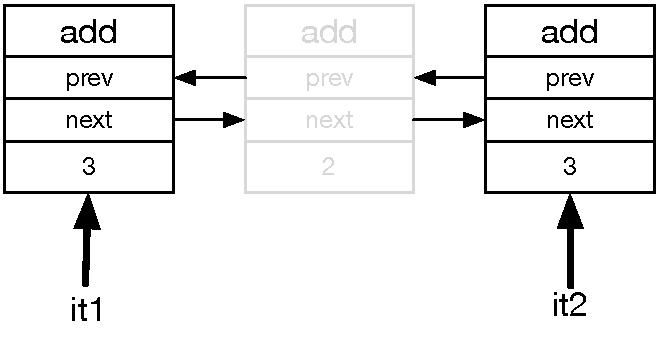
\includegraphics[width=0.8\linewidth]{figures/compiler/update2}
\end{minipage}
\begin{minipage}{.5\textwidth}
   \centering
   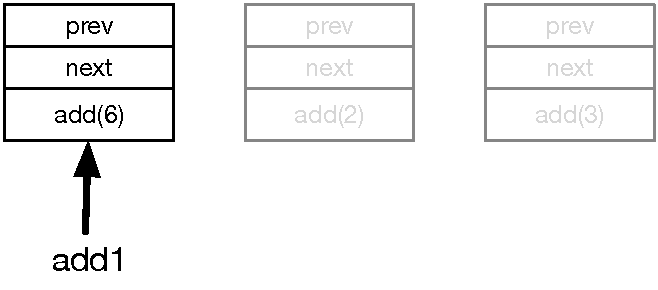
\includegraphics[width=0.8\linewidth]{figures/compiler/update3}
\end{minipage}
\mycap{Executing the add rule. First, the two iterators point to
   the first and second facts and the former is updated while the latter is
   consumed. The second iterator then moves to the next fact and the first fact is
   updated again, now to the value \code{6}, the expected result.}
\label{fig:local:update_add}
\end{figure}

\subsection{Comprehensions}

Consider the comprehension used in the first rule of the bipartiteness checking
program in Fig.~\ref{language:code:bichecking}:

\begin{Code}
visit(A, P),
uncolored(A)
   -o {B | !edge(A, B) -o visit(B, next(P))},
      colored(A, P).
\end{Code}

The attentive reader will remember that comprehensions are sub-rules, therefore
they should be compiled like normal rules. Comprehensions must also derive all
possible combinations. However, the rule itself must return if the
comprehension's RHS derives a fact that is used by a higher priority rule. The
example rule does not need to return since it has the highest priority and the
\code{visit} facts derived in the comprehension are contained in other nodes.
The code for the rule is shown below:

\begin{LineCode}
colored_list <- linked_list("colored")
visit_list <- linked_list("visit")
uncolored_list <- linked_list("uncolored")
visit <- visit_list.head()
while(visit is valid)
{
   uncolored <- uncolored_list.head()
   while(uncolored is valid)
   {
      // Comprehension code.
      edge_trie <- trie("edge")
      edge <- edge_trie.first()
      while(edge is valid)
      {
         new_visit <- create_fact("visit") // New visit fact.
         new_visit.set_int(1, next(visit.get_int(1)))
         // Send fact to B.
         send_fact(new_visit, edge.get_node(1))
         edge <- edge.next()
      }
      new_colored <- create_fact("colored")
      new_colored.set_int(1, visit.get_int(1))
      colored_list.add(new_colored)
      visit <- visit_list.delete_and_next(visit)
      uncolored <- uncolored_list.delete_and_next(uncolored)
      goto next
   }
   uncolored <- uncolored.next()
next:
   continue
}
\end{LineCode}

Special care must be taken when the comprehension's sub-rule uses the same
predicates that are derived by the main rule. Rule inference must be atomic in
the sense that, after a rule matches, the comprehensions in the rule's RHS can
use the facts that were present before the rule was matched. Consider a rule
with $n$ comprehensions or aggregates, where each $CLHS_i$ and $CRHS_i$ are the
LHS and RHS of the comprehension/aggregate $i$, respectively, and $RHSP$
represents the atomic propositions found in rule's RHS. The formula used by the
compiler to detect conflicts between predicates is the following:

\[
\bigcup^{n}_i[CLHS_i \cap RHSP] \cup \bigcup^{n}_i [CLHS_i \cap \bigcup^{n}_j[CRHS_j]]
\]

If the result of the formula is not empty, then the compiler disables
optimizations for the conflicting predicates and derives the corresponding facts
into a temporary data structure before being added into the database data
structures. As an example, consider the following rule:

\begin{Code}
update(A),
!edge(A, B)
   -o {P | points(A, B, P) -o update(B)},
      points(A, B, 1).
\end{Code}

We have $n = 1$ comprehensions, where $CLHS_0 = $ \code{points(A, B, P)},
$CRHS_0 =$ \code{update(B)}, and $RHSP = $ \code{points(A, B, 1)}. There is a
conflict because $CLHS_0 \cap RHSP = \{\mathtt{points}\}$, which requires
\code{points(A, B, 1)} to be derived after the comprehension or be stored in a
temporary data structure to avoid conflicts with the comprehensions, which could
consume the newly derived fact. Fortunately, most rules in LM programs do not
show these kinds of conflicts and thus can be fully optimized.

\subsection{Aggregates}

Aggregates are similar to comprehensions. They are also sub-rules but a value is
accumulated for each combination of the sub-rule. After all the combinations are
derived, a final RHS term is derived with the accumulated value. Consider the
following rule that computes a PageRank value by aggregating all neighbors
PageRank values:

\begin{Code}
update(A),
pagerank(A, OldRank)
      -o [sum => V; B | neighbor-pagerank(A, B, V) -o neighbor-pagerank(A, B, V)
            -> pagerank(A, damping/P + (1.0 - damping) * V)].
\end{Code}

The variable \code{V} is initialized to \code{0.0} and sums all the PageRank
values of the neighbors as seen in the code below. The aggregate value is then
used to update the second argument of the initial \code{pagerank} fact.

\begin{LineCode}
pagerank_list <- linked_list("pagerank")
update_list <- linked_list("update")
neighbor_pagerank_list <- linked_list("neighbor_pagerank_list")
pagerank <- pagerank_list.head()
while(pagerank is valid)
{
   update <- update_list.head()
   while(update is valid)
   {
      V <- 0.0
      neighbor_pagerank <- neighbor_pagerank_list.head()
      while(neighbor_pagerank is valid)
      {
         V <- V + neighbor_pagerank.get_float(2)
         neighbor_pagerank <- neighbor_pagerank.next()
      }
      // RHS of the aggregate
      pagerank.set_float(1, damping / P + (1.0 - damping) * V)
      update <- update_list.delete_and_next(update)
      goto next
   }
   pagerank <- pagerank.next()
next:
   continue
}
\end{LineCode}



\section{Chapter Summary}

In this chapter, we gave an overview of LM's implementation, including the
compiler and the virtual machine. We focused on the sequential aspects of the
implementation, namely, the data structures used for manipulating facts and how
the compiler turns logical rules into efficient code. In the next chapter, we
focus on the parallel aspects of the virtual machine and present an evaluation
of the performance and scalability of the implementation.

\chapter{Multicore Implementation: Parallelism and Optimizations}\label{chapter:implementation}
The compilation and runtime system described in
Chapter~\ref{chapter:implementation} requires ysome changes in both the compiler
and in the runtime system to support thread-based facts.

\subsection{Compiler}

The compiler needs to recognize rules that use thread facts. For thread rules,
the compiler checks if the rule's body is using facts from the same thread by
checking the first argument of each fact. For mixed rules, the rule's body may
use a thread \code{T} and a node \code{A} and all the node facts have to use
\code{A}, while all threads facts must use \code{T} as the first argument. If
the programmer was to retrieve either the thread or the node for the current
computation, she may use \code{running(T, A)}.

Once rules are type checked, the iteration code for thread-based facts
needs to change. The database iterator will refer to the current thread in order to
fetch candidate facts since using the standard node database will return an
empty iterator. The runtime API used for inserting thread facts is also
different since they have to be added to the thread's database.

\subsection{Runtime}

Each thread has its own database of facts that is identical to a regular node
but only contains thread predicates. The major difference between a regular node
and a thread node is that a thread node is never put into the work queue of its
thread. As shown in the updated work loop presented in
Fig.~\ref{alg:threads:work_loop}, the thread node executes alongside the regular
node when $TH.process\_node$ is called. It is also important to note that,
before a thread becomes idle, it may have potential candidate thread rules that
are now derivable because another thread has derived thread facts in the current
thread. Note that it is entirely possible to have programs that only deal with
thread facts. These kinds of programs use only explicit parallelism.

\begin{figure}
\begin{algorithm}[H]
\KwData{Thread TH, THREADS}
\While{true}{
  $node \longleftarrow TH.work\_queue.pop\_node()$ \;
  \uIf{$node$}{
        \tcc{Have to use the thread's node}
        \underline{$TH.process\_node(node, TH.my\_node)$}\;
  }
  \Else{
     $target \longleftarrow random(len(THREADS))$\;
     $i \longleftarrow 0$\;
     \For{$i < len(THREADS)$}{
        $target \longleftarrow (target + 1) \% len(THREADS)$\;
        $nodes = THREADS[target].steal\_half()$\;
        \If{$len(nodes) > 0$}{                                                                                                    $TH.work\_queue.add\_to\_queue(nodes)$\;
           break\;
        }
        $i \longleftarrow i + 1$\;
     }
     \If{$len(TH.work\_queue) == 0$}{
        \tcc{The thread's node may have candidate rules using incoming thread facts}
        \underline{$TH.process\_node(nil, TH.my\_node)$}\;
        $TH.become\_idle()$\;
        \If{$TH.synchronize\_termination()$}{
           \Return{}\;
        }
        $TH.become\_active()$\;
     }
  }
}
\end{algorithm}
\caption{Thread work loop updated to take into account thread-based facts.
New and modified code is underlined.}
\label{alg:threads:work_loop}
\end{figure}

Thread facts also add points of synchronization the runtime system. For
instance, when a rule derives a new thread fact on another thread, it needs to
synchronize with that thread (using locks) to add the facts to the thread's
database.

\subsubsection{Matching Rules}

Matching rules using thread facts requires special care since some rules may
require both facts from a node and from a thread. Before a node is executed, the
matching engine of the regular node is updated to take into account the facts in
the thread. If the mixed rules are activated, they need to be executed, even if
they have failed under a different node. The reason is simple: the rule
constraints may now hold under the current node's database and therefore the
rule needs to be executed again.

\subsection{Graph Of Threads}

We added several helpful predicates that allow the programmer to inspect the
graph of threads and reason about the state of computation as it relates to
threads.

\begin{itemize}
   \item \code{\bang thread-list(T, L)}: Fact instantiated in all threads where
      \code{L} is a list of all threads executing in the system.

   \item \code{\bang other-thread(T1, T2)}: Connects thread \code{T1} to all the
      other threads \code{T2} executing in the system.

   \item \code{\bang leader-thread(T, TLeader)}: Fact instantiated in all
      threads where \code{TLeader} refers to a selected thread (usually the
      first thread in \code{L} of \code{\bang thread-list(T, L)}).

   \item \code{running(T, A)}: Used to retrieve the current node \code{A}
      running on thread \code{T}.
\end{itemize}

With the exception of \code{running}, every other fact is added at the beginning
of the program as a persistent axiom.


\chapter{Logical Foundations: Abstract Machine}
\newcommand{\mz}{\m{match} \;}
\newcommand{\tab}[0]{\;\;\;\;}
\newcommand{\dz}{\m{derive} \;}
\newcommand{\comp}[0]{\m{comp} \;}
\newcommand{\az}{\m{apply} \;}
\newcommand{\doz}{\m{run} \;}
\newcommand{\seqnocut}[3]{#1 ; #2 \Rightarrow #3}
\newcommand{\defeq}{\buildrel\triangle\over =}
\newcommand{\compr}[1]{\m{def} \; #1}

\newcommand{\mo}{\m{match}_1 \;}
\newcommand{\cont}{\m{cont} \;}
\newcommand{\contc}{\m{contc} \;}
\newcommand{\done}{\m{derive}_1 \;}
\newcommand{\doo}{\m{run}_1 \;}
\newcommand{\mc}[0]{\m{match}_c \; }
\newcommand{\dall}[0]{\m{fix} \; }
\newcommand{\strans}[0]{\m{strans} \;}
\newcommand{\dc}{\m{derive}_c \;}
\newcommand{\ao}{\m{apply}_1 \;}

This chapter provides a brief overview of the proof theoretic basis behind \lang and the dynamic semantics
of the language. First, we will present the subset of linear logic from which \lang is built on. Second, we present the high level dynamic semantics (how rules are evaluated) followed by the low level dynamics, a close representation of how to virtual machine runs. Finally, we give an overview of the soundness proof of the low level semantics.

\section{Linear Logic}

\lang differs greatly from other Datalog-like languages due to the use of linear logic~\cite{Girard95logic:its}. Traditional forward-chaining logic programming languages make only use of classical logic, in which derived facts are true forever. Many ad-hoc extensions~\cite{Liu98extendingdatalog,Ludascher95alogical} have been devised in the past to support state updates in Datalog, but most are extra-logical which makes it harder to reason about programs.
\lang uses linear logic as its foundation, therefore state updates are completely natural to the language.

We use a small subset of the original linear logic proof system along with an extension for definitions to improve
the expressiveness of the language. We summarize the connectives used in Table~\ref{table:linear}
and how they are related to the \lang syntax.

\begin{table*}
   \begin{center}
\resizebox{16cm}{!}{
    \begin{tabular}{ | l | l || l | l | l |}
    \hline
    Connective                   & Description                                      & \lang Syntax                                  & \lang Place     & \lang Example                                  \\ \hline \hline
    $\emph{fact}(\hat{x})$       & Linear facts.                                    & $fact(\hat{x})$                               & Body or Head    & \texttt{path(A, P)}                            \\ \hline
    $\bang \emph{fact}(\hat{x})$ & Persistent facts.                                & $\bang fact(\hat{x})$                         & Body or Head    & \texttt{$\bang$edge(X, Y, W)}                  \\ \hline
    $1$                          & Represents rules with an empty head.             & $1$                                           & Head            & \texttt{1}                                     \\ \hline
    $A \otimes B$                & Connect two expressions.                         & $A, B$                                        & Body and Head   & \texttt{path(A, P), edge(A, B, W)}             \\ \hline
    $\forall x. A$               & To represent variables defined inside the rule.  & Please see $A \lolli B$                       & Rule            & \texttt{path(A, B) $\lolli$ reachable(A, B)}   \\ \hline
    $\exists x. A$               & Instantiates new node variables.                 & $exists \; \widehat{x}. (B)$                  & Head            & \texttt{exists A.(path(A, P))}                 \\ \hline
    $A \lolli B$                 & $\lolli$ means "linearly implies".               & $A \lolli B$                                  & Rule            & \texttt{path(A, B) $\lolli$ reachable(A, B)}   \\
                                 & $A$ is the body and $B$ is the head.             &                                               &                 &                                                \\ \hline
    $\m{def} A. B$               & Extension called definitions.                    & $\{\; \widehat{x} \; | \; A \; | \; B \; \}$  & Head            & \texttt{\{B | !edge(A, B) | visit(B)\}}        \\
                                 & Used for comprehensions and aggregates.          &                                               &                 &                                                \\ \hline
    \end{tabular}
}
\end{center}
\caption{Connectives from Linear Logic used in \lang.}
\label{table:linear}
\end{table*}

The sequent calculus for our linear logic fragment is shown in Fig.~\ref{linear_logic}.
The sequent has the form $\Psi ; \seqnocut{\Gamma}{\Delta}{C}$, where $\Psi$ is the typed
term context used in the quantifiers, $\Gamma$ is the multi-set of persistent terms, $\Delta$
is the multi-set of linear terms and $C$ is the term we want to prove.

Most connectives in our fragment are standard and well known, except for the $\compr{A}$ connective. This
connective is a definition that can be unfolded recursively and is used to logically justify
comprehensions and aggregates. We took inspiration from Baelde's work on least and greatest fixed points
in linear logic~\cite{Baelde:2012:LGF:2071368.2071370}. Baelde's system goes beyond simple recursive
definitions and allows proofs using induction and co-induction in linear logic. Fortunately,
the proof system satisfies cut-elimination which makes it consistent. 

In a comprehension, we want to apply an implication as many times as possible matches we can do
using the current database. One way to formally describe comprehensions would be to use persistent
rules that would be used a few times and then would be forgotten. A more reasonable approach is to use
definitions. Given a comprehension $C = \{ \; \widehat{x} \; | \; A \; | \; B \; \}$ with a body $A$ and a head $B$, then we can build the following definition:

\[
\compr{C} \defeq 1 \with ((A \lolli B) \otimes \compr{C})
\]

We can unfold $\compr{C}$ to either stop (by selecting $1$) or get a new linear implication $A \lolli B$
to apply the comprehension once. Because we also get another $\compr{C}$ by selecting the right hand side,
the comprehension can be applied again, recursively.

Aggregates work identically, but they need an extra argument to accumulate the aggregated value. If a sum aggregate $C$ has the form $[\;\m{sum} \Rightarrow y \; | \; \widehat{x} \; | \; A \; | \; B_1 \; | \; B_2 \;]$, then the definition will be as follows:

\[
\compr{C} \; V \defeq (\lambda v. B_2)V \with (\forall x. ((Ax \lolli B_1) \otimes \compr{C} \; (x + V)))
\]

The aggregate is initiated as $\compr{C} \; 0$.

\begin{figure}[ht]
\[
\infer[\one R]
{\Psi ; \seqnocut{\Gamma}{\cdot}{\one}}
{}
\tab
\infer[\one L]
{\Psi ; \seqnocut{\Gamma}{\Delta, \one}{C}}
{\Psi ; \seqnocut{\Gamma}{\Delta}{C}}
\]

\[
\infer[\with R]
{\Psi ; \seqnocut{\Gamma}{\Delta}{A \with B}}
{\Psi ; \seqnocut{\Gamma}{\Delta}{A} & \seqnocut{\Gamma}{\Delta}{B}}
\tab
\infer[\with L_1]
{\Psi ; \seqnocut{\Gamma}{\Delta, A \with B}{C}}
{\Psi ; \seqnocut{\Gamma}{\Delta, A}{C}}
\tab
\infer[\with L_2]
{\Psi ; \seqnocut{\Gamma}{\Delta, B \with B}{C}}
{\Psi ; \seqnocut{\Gamma}{\Delta, B}{C}}
\]

\[
\infer[\otimes R]
{\Psi ; \seqnocut{\Gamma}{\Delta, \Delta'}{A \otimes B}}
{\Psi ; \seqnocut{\Gamma}{\Delta}{A} & \seqnocut{\Gamma}{\Delta}{B}}
\tab
\infer[\otimes L]
{\Psi ;\seqnocut{\Gamma}{\Delta, A \otimes B}{C}}
{\Psi ; \seqnocut{\Gamma}{\Delta, A, B}{C}}
\]

\[
\infer[\lolli R]
{\Psi ; \seqnocut{\Gamma}{\Delta}{A \lolli B}}
{\Psi ; \seqnocut{\Gamma}{\Delta, A}{B}}
\tab
\infer[\lolli L]
{\seqnocut{\Gamma}{\Delta, \Delta', A \lolli B}{C}}
{\Psi ; \seqnocut{\Gamma}{\Delta}{A} &
   \Psi ; \seqnocut{\Gamma}{\Delta', B}{C}}
\]

\[
\infer[\forall R]
{\Psi ; \seqnocut{\Gamma}{\Delta}{\forall n:\tau. A}}
{\Psi, m:\tau ; \seqnocut{\Gamma}{\Delta}{A\{m/n\}}}
\tab
\infer[\forall L]
{\Psi ; \seqnocut{\Gamma}{\Delta, \forall n:\tau. A}{C}}
{\Psi \vdash M : \tau & \Psi ; \seqnocut{\Gamma}{\Delta, A\{M/n\}}{C}}
\]

\[
\infer[\exists R]
{\Psi ; \seqnocut{\Gamma}{\Delta}{\exists n: \tau. A}}
{\Psi \vdash M : \tau &
   \Psi ; \seqnocut{\Gamma}{\Delta}{A \{M/n\}}}
\tab
\infer[\exists L]
{\Psi ; \seqnocut{\Gamma}{\Delta, \exists n:\tau. A}{C}}
{\Psi, m:\tau ; \seqnocut{\Gamma}{\Delta, A\{m/n\}}{C}}
\]

\[
\infer[\bang R]
{\Psi ; \seqnocut{\Gamma}{\cdot}{\bang A}}
{\Psi ; \seqnocut{\Gamma}{\cdot}{A}}
\tab
\infer[\bang L]
{\Psi ; \seqnocut{\Gamma}{\Delta, \bang A}{C}}
{\Psi ; \seqnocut{\Gamma, A}{\Delta}{C}}
\tab
\infer[\m{copy}]
{\Psi ; \seqnocut{\Gamma, A}{\Delta}{C}}
{\Psi ; \seqnocut{\Gamma, A}{\Delta, A}{C}}
\]

\[
\infer[\m{def} \; R]
{\Psi ; \seqnocut{\Gamma}{\Delta}{\compr{A'}}}
{\Psi ; \seqnocut{\Gamma}{\Delta}{B\theta} &
 A \defeq B & A' \doteq A\theta}
\tab
\infer[\m{def} \; L]
{\Psi ; \seqnocut{\Gamma}{\Delta, \compr{A'}}{C}}
{
   \Psi ; \seqnocut{\Gamma}{\Delta, B\theta}{C} & A \defeq B & A' \doteq A\theta
}
\]
\caption{Linear logic fragment used in \lang.}\label{linear_logic}
\end{figure}

\section{High Level Dynamic Semantics}

In this section, we are going to present the high level dynamic semantics of \lang. The semantics
formalize the mechanism of matching rules and deriving new facts. The high level semantics
present a simplified overview of the dynamics of the language that are closer to the formalism
of linear logic present in Fig.~\ref{linear_logic} than the implementation principles of our
virtual machine.

Both the high level and low level semantics do not model the use of variable bindings when matching
facts from the database. The formalization of bindings tends to complicate the formal system and it is not
necessary for a good understanding of the system. Instead, we assume that all facts of
type $\emph{fact}(\hat{x})$ do not have the argument $\hat{x}$.

Starting from the linear logic fragment presented earlier, we consider $\Gamma$ and $\Delta$ the database
of our program. $\Gamma$ contains the database of persistent facts while $\Delta$ the database of linear
facts. We assume that the rules of the program are persistent linear implications of the form
$\bang (A \lolli B)$ that can be used several times. However, we do not put the rules in the $\Gamma$
context but in a separate context $\Phi$.

The main idea of the dynamic semantics is to ignore the right side of the sequent calculus
and use inversion on the $\Delta$ and $\Gamma$ context so that we only have atomic facts.
To apply rules we use chaining by focusing on one of the derivation rules in $\Phi$. Note
that in the focusing process we assume that all the atoms (facts) are positive thus the chaining
becomes a forward chaining process.

\subsubsection{Application}

The main judgment of the system is $\doz \Gamma; \Delta; \Phi \rightarrow \Xi'; \Delta'; \Gamma'$.
$\Gamma$, $\Delta$ and $\Phi$ have the meaning explained before, while $\Xi'$, $\Delta'$ and $\Gamma'$
are output multi-sets from applying one of the rules in $\Phi$. $\Xi'$ is the set of consumed linear
resources, $\Delta'$ is the set of derived linear facts and $\Gamma'$ is the set of derived persistent
facts. Note that for the high level semantics there is no concept of rule priority, so we pick a rule
non-deterministically.

The judgment $\az \Gamma ; \Delta ; A \lolli B \rightarrow \Xi'; \Delta'; \Gamma'$ will attempt to apply
the derivation rule $A \lolli B$. To do this, it splits the $\Delta$ context into $\Delta_1$ and $\Delta_2$, namely the
set of linear resources consumed to match the body of the rule ($\Delta_1$) and the remaining linear facts ($\Delta_2$).
Again, the set of resources needed to match the body of the rule is guessed. The low level dynamic semantics will
deterministically determine $\Delta_1$.

\[
\infer[\az rule]
{\az \Gamma ; \Delta_1, \Delta_2 ; A \lolli B \rightarrow \Xi' ; \Delta' ; \Gamma'}
{\mz \Gamma ; \Delta_1 \rightarrow A & \dz \Gamma ; \Delta_2; \Delta_1; \cdot ; \cdot ; B \rightarrow \Xi' ; \Delta' ; \Gamma'}
\]

\[
\infer[\doz rule]
{\doz \Gamma ; \Delta ; R, \Phi \rightarrow \Xi' ; \Delta' ; \Gamma'}
{\az \Gamma ; \Delta ; R \rightarrow \Xi' ; \Delta' ; \Gamma'}
\]

\subsubsection{Match}

The $\mz \Gamma ; \Delta \rightarrow C$ judgment essentially uses the right ($R$) rules of the original
linear logic fragment in order to match all facts using $\Gamma$ and $\Delta$. We must consume all the linear facts in
the multi-set $\Delta$ when matching $C$. The context $\Gamma$ may be used to match persistent terms in $C$ but such
facts are never consumed since they are persistent.

\[
\infer[\mz 1]
{\mz \Gamma; \cdot \rightarrow 1}
{}
\tab
\infer[\mz p]
{\mz \Gamma; p \rightarrow p }
{}
\tab
\infer[\mz \bang p]
{\mz \Gamma, p; \cdot \rightarrow \bang p}
{}
\]

\[
\infer[\mz \otimes]
{\mz \Gamma; \Delta_1, \Delta_2 \rightarrow A \otimes B}
{\mz \Gamma; \Delta_1 \rightarrow A & \mz \Delta_2 \rightarrow B}
\]

\subsubsection{Derivation}

The derivation judgment has the form $\dz \Gamma ; \Delta ; \Xi ; \Gamma_1 ; \Delta_1 ; \Omega \rightarrow \Xi'; \Delta'; \Gamma'$ with the following meaning:

\begin{enumerate}
   \item[$\Gamma$] the multi-set of persistent resources in the database.
   \item[$\Delta$] the multi-set of linear resources in the database not yet consumed.
   \item[$\Xi$] the multi-set of linear resources that have been consumed while matching the body of the rule, matching comprehensions or aggregates.
   \item[$\Gamma_1$] the multi-set of persistent facts that have been derived using the current rule.
   \item[$\Delta_1$] the multi-set of linear facts that have been derived using the current rule.
   \item[$\Omega$] an ordered list contain the terms of the head of rule that still need to be derived. We start with the head of the rule $B$ that is continuously deconstructed to derive all the facts of the rule.
   \item[$\Xi'$] the consumed linear facts to apply this rule.
   \item[$\Delta'$] the derived linear facts.
   \item[$\Gamma'$] the derived persistent facts.
\end{enumerate}

We did not include the aggregates here because they are similar to comprehensions. The main rule to
derive comprehensions is $\dz comp$. It unfolds the comprehension which it can be then either
applied ($\dz \with R$ followed by $\dz \lolli$) or not ($\dz \with L$). The high level semantics
do not take into account the contents of the database to determine how many times a comprehension
should be applied because it is entirely non-deterministic.



\[
\infer[\dz p]
{\dz \Gamma ; \Delta ; \Xi ; \Gamma_1 ; \Delta_1 ; p, \Omega \rightarrow \Xi' ; \Delta' ; \Gamma'}
{\dz \Gamma ; \Delta ; \Xi ; \Gamma_1 ; p, \Delta_1 ; \Omega \rightarrow \Xi' ; \Delta' ; \Gamma'}
\]

\[
\infer[\dz \bang p]
{\dz \Gamma ; \Delta ; \Xi ; \Gamma_1 ; \Delta_1 ; \bang p, \Omega \rightarrow \Xi' ; \Delta' ; \Gamma'}
{\dz \Gamma ; \Delta ; \Xi ; \Gamma_1, p ; \Delta_1 ; \Omega \rightarrow \Xi' ; \Delta' ; \Gamma'}
\]

\[
\infer[\dz \otimes]
{\dz \Gamma ; \Delta ; \Xi ; \Gamma_1 ; \Delta_1 ; A \otimes B, \Omega \rightarrow \Xi' ; \Delta' ; \Gamma'}
{\dz \Gamma ; \Delta ; \Xi ; \Gamma_1 ; \Delta_1 ; A, B, \Omega \rightarrow \Xi' ; \Delta' ; \Gamma'}
\]

\[
\infer[\dz 1]
{\dz \Gamma ; \Delta ; \Xi ; \Gamma_1; \Delta_1 ; 1, \Omega \rightarrow \Xi' ; \Delta' ; \Gamma'}
{\dz \Gamma ; \Delta ; \Xi ; \Gamma_1; \Delta_1 ; \Omega \rightarrow \Xi' ; \Delta' ; \Gamma'}
\]

\[
\infer[\dz end]
{\dz \Gamma ; \Delta ; \Xi' ; \Gamma' ; \Delta' ; \cdot \rightarrow \Xi' ; \Delta' ; \Gamma'}
{}
\]


\[
\infer[\dz comp]
{\dz \Gamma ; \Delta ; \Xi ; \Gamma_1 ; \Delta_1 ; \comp A \lolli B, \Omega \rightarrow \Xi' ; \Delta' ; \Gamma'}
{\dz \Gamma ; \Delta ; \Xi ; \Gamma_1 ; \Delta_1 ; 1 \with (A \lolli B \otimes \comp A \lolli B), \Omega \rightarrow \Xi' ; \Delta' ; \Gamma'}
\]

\[
\infer[\dz \lolli]
{\dz \Gamma ; \Delta_a, \Delta_b ; \Xi ; \Gamma_1 ; \Delta_1 ; A \lolli B, \Omega \rightarrow \Xi' ; \Delta' ; \Gamma'}
{\mz \Gamma ; \Delta_a \rightarrow A & \dz \Gamma ; \Delta_b ; \Xi, \Delta_a ; \Gamma_1 ; \Delta_1 ; B, \Omega \rightarrow \Xi' ; \Delta' ; \Gamma'}
\]

\[
\infer[\dz \with L]
{\dz \Gamma ; \Delta ; \Xi ; \Gamma_1 ; \Delta_1 ; A \with B, \Omega \rightarrow \Xi' ; \Delta'; \Gamma'}
{\dz \Gamma ; \Delta ; \Xi ; \Gamma_1 ; \Delta_1 ; A, \Omega \rightarrow \Xi' ; \Delta'; \Gamma'}
\]

\[
\infer[\dz \with R]
{\dz \Gamma ; \Delta ; \Xi ; \Gamma_1 ; \Delta_1 ; A \with B, \Omega \rightarrow \Xi' ; \Delta' ; \Gamma'}
{\dz \Gamma ; \Delta ; \Xi ; \Gamma_1 ; \Delta_1 ; B, \Omega \rightarrow \Xi' ; \Delta' ; \Gamma'}
\]

\section{Low Level Dynamic Semantics}

The low level dynamic semantics removes all the non-deterministic choices in the previous dynamics
and makes them deterministic. The new semantics will do the following:

\begin{itemize}
   \item Match rules by priority order;
   \item Determine the set of linear facts needed to match either the body of the rule or the body of comprehensions without guessing;
   \item Apply as many comprehensions as the database allows.
\end{itemize}

The complete set of inference rules for the semantics are presented in Appendix~\ref{low_level_semantics}.

\subsection{Continuation Frames}

The new semantics introduce the concept of continuation frames. Continuation frames are choice points
created when we need to match some fact expression against the database. The frame considers all the facts
relevant to the fact expression given the current variable bindings, that may or not fail during the remaining matching process. Note that we assume
that facts have arguments and variable bindings although this is not explicit in the semantics
presented in the Appendix.
The frame contains enough state to resume the matching process at the time of its creation and
to select the next candidate fact from the database.

If at some point we cannot match a fact expression due to a wrong choice that happened earlier on,
we need to backtrack (judgment $\m{cont}$ or $\m{contc}$). Since we keep all the continuation frames in a continuation stack,
we grab the top frame and select the next fact candidate to complete the matching process.
If all candidates are exhausted, we pop the current frame and try the next one.

By using this matching mechanism, we can determine which facts need to be used to match a rule.
The virtual machine implemented for \lang works pretty much in the same way, by iterating over
the available facts at each choice point and then committing to the rule if the matching process
succeeds.

\subsubsection{Continuation Frame Format}

We have two continuation frames: linear continuation frames and persistent continuation frames.

Linear frames have the form $(\Delta; \Delta_{next}; p; \Omega; \Xi; \Lambda; \Upsilon)$, where:

\begin{enumerate}
   \item[$\Delta$] Contains all the linear resources available at this choice point minus the other facts that can used to match $p$ (they are in $\Delta_{next}$).
   \item[$\Delta_{next}$] The available options to match fact $p$ if the matching fails. When backtracking, we move one fact from $\Delta_{next}$ into $\Delta$.
   \item[$p$] The fact expression that created this frame.
   \item[$\Omega$] Ordered list with the remaining terms we have to match to complete the matching process.
   \item[$\Xi$] Multi-set of consumed linear facts up to this choice point.
   \item[$\Lambda$] Multi-set of linear fact expressions already matched. All those terms must have a matching fact in $\Xi$.
   \item[$\Upsilon$] Multi-set of persistent fact expressions already matched. All those terms must have a matching fact in $\Gamma$.
\end{enumerate}

Persistent frames are simpler with the form $[\Gamma_{next}; \Delta; \bang p; \Omega; \Xi; \Lambda; \Upsilon]$, where:

\begin{enumerate}
   \item[$\Gamma_{next}$] The multi-set of available options for $\bang p$ if the current matching process fails.
   \item[$\Delta$] The multi-set of linear resources still available when the frame was created.
   \item[$\bang p$] The fact expression that created this frame.
\end{enumerate}

All the other arguments are equal to the ones used in the linear continuation frame.

\subsection{Rule Priority}

In order to respect rule priority, the low level dynamic semantics first try to match rules with
higher priority. To do this, we use a continuation frame with type $(\Phi, \Delta)$, where $\Phi$
is the list of remaining rules to try and $\Delta$ is the original $\Delta$ context. If the matching
process of the current rule fails, we use this continuation frame to try the next rule in the list.

\subsection{Comprehensions}

The matching process for both comprehensions and aggregates work slightly different than matching the
body of a rule. When the body of a rule is matched, we throw away the continuation stack since we
do not need to backtrack. For comprehensions and aggregates, every time we succeed in matching the body
we have to derive the head (for comprehensions only judgment $\m{derive}_c$) but we need to reuse the
continuation stack to
apply the comprehension (or aggregate) again. This is because the continuation stack contains,
by definition, enough information to allow the comprehension to iterate over all possible matches.

However, one needs to be careful in reusing the continuation stack. If we are matching the body
\texttt{$\bang$a(X), b(X), c(X)} and the continuation stack has three frames (one per fact), we cannot
backtrack to the frame of \texttt{c(X)} since at that point the matching process was assuming that the previous
\texttt{b(X)} linear fact was still unconsumed. Therefore we need to backtrack to the first linear
continuation frame, in this case \texttt{b(X)}. The judgment that performs such task is $\m{fix}$.
Finally, we still have to update the state of every frame
of the new continuation stack in order to remove all consumed facts from the frames ($\m{strans}$).

Note that our continuation stack is split into two stacks: $C$ and $P$. $P$ contains only
persistent continuation frames and is used first. $C$ is used for the first linear continuation frame
that appears during matching. Any persistent frame that appears afterwards is put in $C$. This makes
it easier to detect where the first linear frame is by just removing every frame except the first in $C$.

\section{Soundness Proof}

The soundness theorem proves that if a rule was successfully derived in the low level semantics
then it can also be successfully derived in the high level semantics. The completeness theorem cannot
be proven correct because the low level semantics lack the non-determinism of the high level semantics.

The first main lemma of the soundness proof proves that if we can match the body
of a rule at the low level then we can also match the rule in the high level system using the same database.

\begin{lemma}[Body Match]
   Given a match $\mo \Gamma; \Delta_1, \Delta_2; \cdot; A; B; \cdot; R \rightarrow \Xi'; \Delta'; \Gamma'$ that is related to $A$, $\Delta_1, \Delta_2$ and $\Gamma$, we get either:
   
   \begin{enumerate}
      \item $\cont \cdot; B; R; \Gamma; \Xi'; \Delta'; \Gamma'$;
      \item $\mz \Delta_2 \rightarrow A$ and $\mo \Gamma; \Delta_1; \Delta_2; \cdot; B; C'; R \rightarrow \Xi'; \Delta'; \Gamma'$ (related)
   \end{enumerate}
\end{lemma}
\begin{proof}
   Use the body match soundness theorem.
\end{proof}

When we say that a match is related to a term $A$ and a database $\Delta_1, \Delta_2, \Gamma$ we mean that
the matching judgment is related to the body $A$ of a rule and the initial database is $\Delta_1, \Delta_2, \Gamma$. Moreover, the continuation stack is related to $A$ and to the database.

The body match lemma tells us that if we start a match of a body $A$ we will either fail (1) and need to try another rule in $R$ or we succeed by building the high level matching judgment $\mz \Delta_2 \rightarrow A$ and reaching the end of the matching process $\mo \Gamma; \Delta_1; \Delta_2; \cdot; B; C'; R \rightarrow \Xi'; \Delta'; \Gamma'$.

This lemma uses a more complicated theorem that is recursively defined through judgments $\m{match}_1$ and $\m{cont}$ that use mutual induction on the size of the continuation stack, the size of the remaining terms
 to match and also the size of alternatives at each continuation frame.
 
The second stepping stone in the soundness proof is the derivation lemma. After we successfully match the
body of a rule, we need to prove that the derivation process (through judgments $\m{derive}_1$) is also
sound. This lemma is as follows:

\begin{lemma}[Derivation]
   If the low level derivation $\done \Gamma; \Delta; \Xi; \Gamma_1; \Delta_1; \Omega \rightarrow \Xi'; \Delta'; \Gamma'$ is true then the high level derivation $\dz \Gamma; \Delta; \Gamma_1; \Delta_1; \Omega \rightarrow \Xi'; \Delta'; \Gamma'$ is also true.
\end{lemma}
\begin{proof}
   Straightforward use of induction on $\Omega$ except for the sub-case of comprehensions and aggregates, where we need to use the comprehension and aggregate theorems to construct the derivation tree using $n$ applications of the corresponding construct.
\end{proof}

In the case of proving the soundness of comprehensions, we use a very identical theorem to the one used
to prove the body match soundness. However, in this case we need to reuse the continuation stack several
times (as many as many comprehensions can be applied). Using induction on the continuation stack, we get
$n$ (where $n \ge 0$) applications of the comprehension and $n \; \m{match}$ and $n \; \m{derive}$ judgments
that can be used to rebuild the derivation tree at the low level by using the $\dz \with L$, $\dz \with R$
and $\dz \lolli$ rules to fold and unfold the comprehension term. The theorem for aggregates works similarly.

\section{Summary}

In this chapter we presented the proof theoretic foundations of \lang.
First, we introduced the linear logic fragment that supports \lang. We then presented the
high level dynamic semantics that was created by interpreting the linear logic fragment using
focusing and chaining. Next, we designed
a formal system called the low level dynamic semantics that mimics the execution of rules in
our virtual machine minus small details.
Finally, we gave a brief overview of the soundness proof of the low level dynamic semantics,
thus proving that our virtual machine is sound in respect to our high level semantics.




\chapter{Coordination: Scheduling and Partitioning}\label{chapter:coordination}
In Chapter~\ref{chapter:implementation}, we saw that the set of nodes
of an LM program is represented as a graph data structure $G = (V, E)$ with nodes $V$
and edges $E$ where $T$ threads perform work. Our implementation also allows
threads to steal nodes from other threads in order to improve load balancing.
However, there are many scheduling details that are left undefined. How should a
thread schedule the computation of its sub-graph? Is node stealing beneficial to
all programs? What is the best sub-graph partitioning for a given LM program?
The answer to all these questions is \emph{coordination}, a mechanism that we
introduce to allow the programmer to specify custom scheduling and node
partitioning policies. This is an important functionality because LM uses linear
logic and thus the order in which nodes are scheduled can impact the performance
and even the results of the program.

\section{Motivation}\label{section:coord:rationale}

To motivate the need for coordination, we use the Single Source Shortest
Path~(SSSP) program, a concise program that can take advantage of custom
scheduling policies to improve its performance.
Figure~\ref{code:shortest_path_program} and Figure~\ref{code:coord:sssp_init}
show a possible implementation in LM, and Fig.~\ref{fig:shortest_path_program}
shows an instance of the program on a particular dataset. Note that in
Section~\ref{section:implementation:performance}, we presented the MSSD program
which is essentially the SSSP program modified to compute multiple shortest
distances.

The SSSP program starts with the declaration of the predicates~
(lines~\ref{line:coord:sssp_pred1}-\ref{line:coord:sssp_pred2}). As usual, the
\code{edge} predicate is a persistent predicate that describes the edges of the
graph, where the third argument is the weight of each edge. Predicate
\code{shortest} represents a valid distance and path from node \code{@1} to the
node in the first argument.  Predicate \code{relax} also represents a valid
path, and, is used to improve the distance in \code{shortest}.  The program
computes the shortest distance from node \code{@1} by improving the distance in
the \code{shortest} facts, until the shortest distance is reached in all nodes.
In Fig.~\ref{code:coord:sssp_init}, we declare an example set of initial facts
for the program: \code{edge} facts describe the graph; \code{shortest(A, +00,
[])} is the initial shortest distance (infinity) for all nodes; and
\code{relax(@1, 0, [@1])} starts the algorithm by setting the distance from
\code{@1} to \code{@1} to be 0.

\begin{figure}[ht]
\begin{LineCode}[commandchars=\*\#\&]
type edge(node, node, int).*label#line:coord:sssp_pred1&*hfill// Predicate declaration
type linear shortest(node, int, list int).
type linear relax(node, int, list int).*label#line:coord:sssp_pred2&

shortest(A, D1, P1), D1 > D2, relax(A, D2, P2)*label#line:coord:sssp_first1&*hfill// Rule 1: newly improved path
   -o shortest(A, D2, P2),
      {B, W | !edge(A, B, W) -o relax(B, D2 + W, P2 ++ [B])}.*label#line:coord:sssp_first2&

shortest(A, D1, P1), D1 <= D2, relax(A, D2, P2)*label#line:coord:sssp_second1&*hfill// Rule 2: longer path
   -o shortest(A, D1, P1).*label#line:coord:sssp_second2&
\end{LineCode}
\mycap{Single Source Shortest Path program code.}
\label{code:shortest_path_program}
\end{figure}

\begin{figure}[ht]
\begin{LineCode}[commandchars=\*\#\&]
!edge(@1, @2, 3). !edge(@1, @3, 1).
!edge(@3, @2, 1). !edge(@3, @4, 5).
!edge(@2, @4, 1).
shortest(A, +00, []).
relax(@1, 0, [@1]).
\end{LineCode}
\mycap{Initial facts for the SSSP program.}
\label{code:coord:sssp_init}
\end{figure}

\iffalse
\begin{figure}[ht]
\begin{LineCode}[commandchars=\*\#\&]
!edge(@1, @2, 3). !edge(@1, @3, 1).
!edge(@3, @2, 1). !edge(@3, @4, 5).
!edge(@2, @4, 1).
shortest(@1, 0, []).
shortest(@2, 2, [@1, @3, @2]).
shortest(@3, 1, [@1, @3]).
shortest(@4, 3, [@1, @3, @2, @4]).
\end{LineCode}
\mycap{Final database of facts for the SSSP program.}
\label{code:coord:sssp_end}
\end{figure}
\fi
\begin{figure}
\begin{center}
   \begin{subfigure}[b]{0.49\textwidth}
      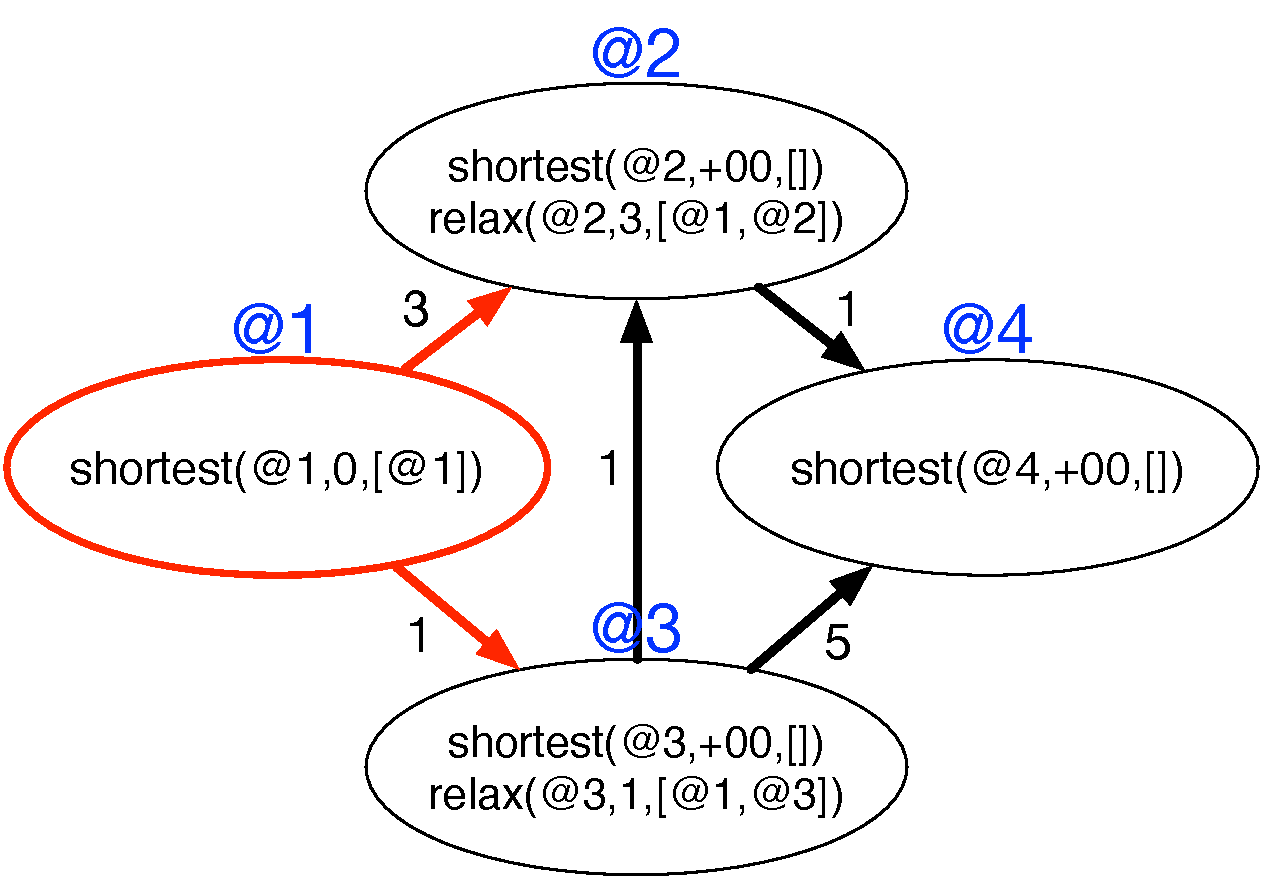
\includegraphics[width=\textwidth]{figures/sssp/shortest2}
      \mycap{}
   \end{subfigure}
   \begin{subfigure}[b]{0.49\textwidth}
      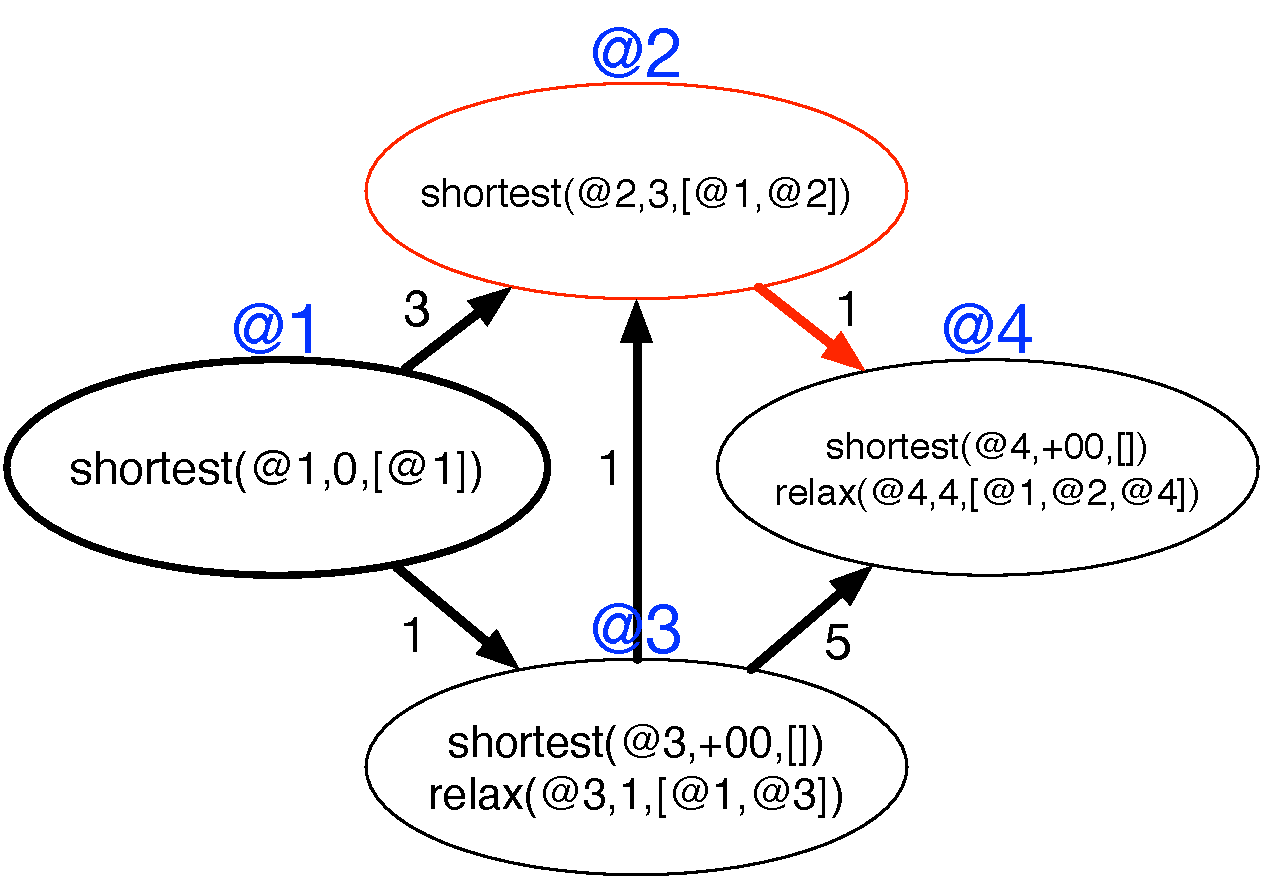
\includegraphics[width=\textwidth]{figures/sssp/shortest3}
      \mycap{}
   \end{subfigure}
   \begin{subfigure}[b]{0.49\textwidth}
      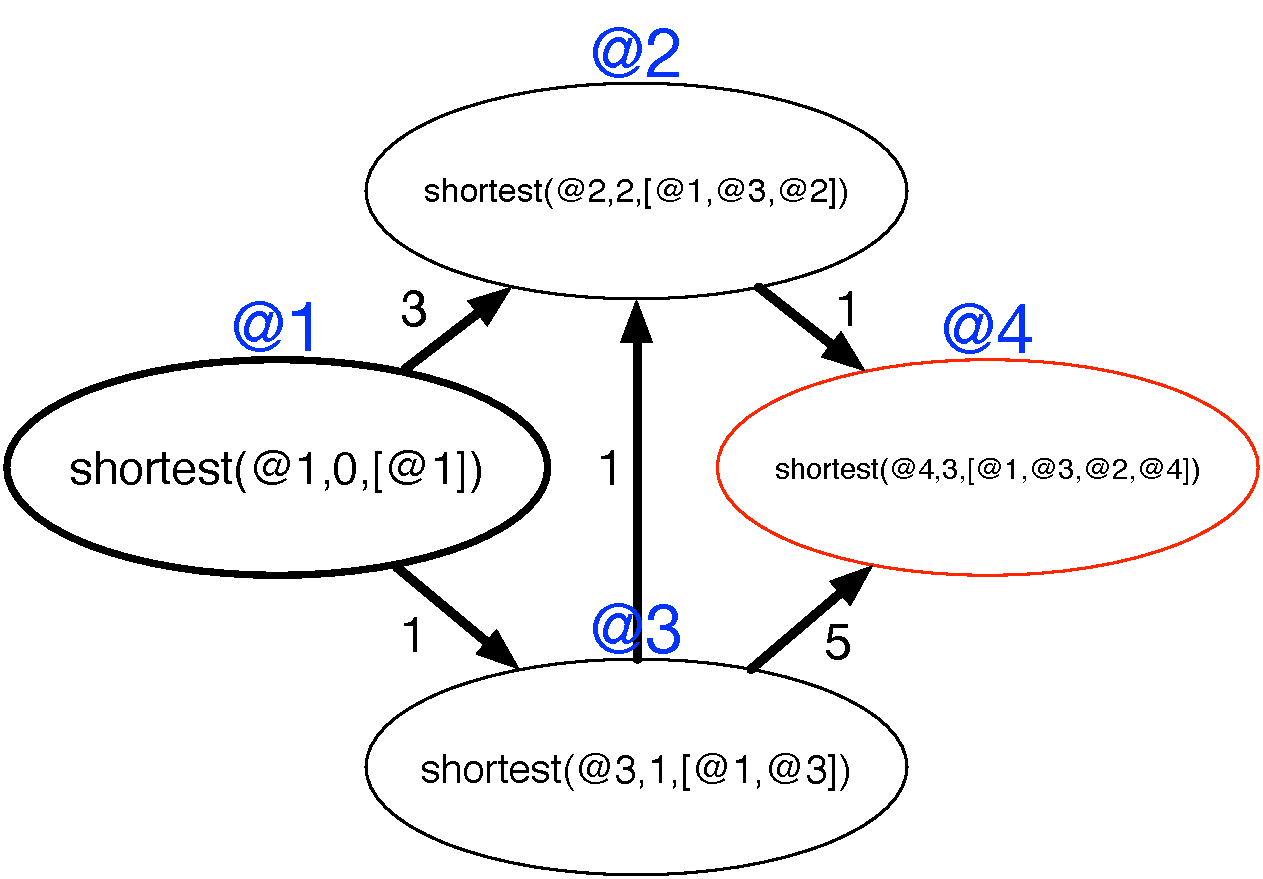
\includegraphics[width=\textwidth]{figures/sssp/shortest8}
      \mycap{}
   \end{subfigure}
\end{center}

\mycap{Graphical representation of an example dataset for the SSSP program: (a) represents the
   program's state after propagating the initial distance at node \code{@1}, followed by (b)
   where the first rule is applied in node \code{@2}, and (c) represents the
   final state of the program, where all the shortest paths have been computed.}

\label{fig:shortest_path_program}
\end{figure}

The first rule of the program
(lines~\ref{line:coord:sssp_first1}-\ref{line:coord:sssp_first2}) reads as
follows: if the current \code{shortest} path \code{P1} with distance \code{D1}
is larger than a new path \code{relax} with distance \code{D2}, then replace the
current shortest path with \code{D2}, delete the new \code{relax} path and
propagate new paths to the neighbors (comprehension at
line~\ref{line:coord:sssp_first2}). The comprehension iterates over the edges of
node \code{A} and derives a new \code{relax} fact for each node \code{B} with
the distance \code{D2 + W}, where \code{W} is the weight of the edge. For
example, in Fig.~\ref{fig:shortest_path_program}(a) we apply rule 1 in node
\code{@1} and two new \code{relax} facts are derived at node \code{@2} and
\code{@3}.  Fig.~\ref{fig:shortest_path_program}(b) is the result after
applying the same rule but at node \code{@2}.

The second rule of the program
(lines~\ref{line:coord:sssp_second1}-\ref{line:coord:sssp_second2}) retracts a
\code{relax} fact that has a longer distance than the current shortest distance
stored in \code{shortest}. There are many opportunities for custom scheduling
in the SSSP program. For instance, after applying rule 1 in
Fig.~\ref{fig:shortest_path_program}(a), it is possible to either apply rules
in either node \code{@2} or node \code{@3}.  This decision depends largely on
implementation factors such as node partitioning and number of threads in the
system. Still, it is easy to prove that, independent of the particular scheduling used, the final
result presented in Fig.~\ref{fig:shortest_path_program}(c) is always achieved.

The SSSP program is concise and declarative but its performance depends on the
order in which nodes are executed. If nodes with greater distances are
prioritized over other nodes, the program will generate more \code{relax} facts
and it will take longer to reach the shortest distances. From
Fig.~\ref{fig:shortest_path_program}, it is clear that the best scheduling is
the following: \code{@1}, \code{@3}, \code{@2} and then \code{@4}, where only 4
\code{relax} facts are generated. If we had decided to process nodes in order
\code{@1}, \code{@2}, \code{@4}, \code{@3}, \code{@4}, \code{@2}, then 6
\code{relax} facts would have been generated.  The optimal solution for SSSP is
to schedule the node with the shortest distance, which is essentially the
Dijkstra shortest path algorithm~\cite{Dijkstra}. Note how it is possible to
change the complexity of the algorithm by simply changing the order of node
computation, but still retain the same declarative nature of the program.



\section{Types of Facts}

LM introduces the concept of coordination that allows the programmer to write
code that changes how the runtime system schedules and partitions the set of
available nodes across the threads of execution. Beyond the distinction between
linear and persistent facts, LM further classifies facts into 3 categories:
\emph{computation facts}, \emph{structural facts} and \emph{coordination facts}.
Predicates are also classified accordingly.

Computation facts are regular facts used to represent the program state. In
Fig.~\ref{code:shortest_path_program}, \texttt{relax} and \texttt{shortest} are
both computation facts.

Structural facts describe information about the connections between the nodes in
the graph. In Fig.~\ref{code:shortest_path_program}, \texttt{edge} facts are
structural since the corresponding \texttt{edge} is used for communication
between nodes.  Note that structural facts can also be seen as computation facts
since they are heavily used in the program's logic.

\emph{Coordination facts} are classified into \emph{scheduling facts} and
\emph{partitioning facts} and allow the programmer to change how the runtime
schedules nodes and how it partitions the nodes among threads of execution,
respectively. Coordination facts can be used either in the LHS, RHS or both.
This allows scheduling and partition decisions to be made based on the state of
the program and on the state of the underlying machine.  In this fashion, we
keep the language declarative because we reason logically about the state of
execution, without the need to introduce extra-logical operators into the
language that would generate significant issues when proving properties about
the programs.

Both scheduling and partitioning facts can be further classified into two kinds
of facts: \emph{sensing facts} and \emph{action facts}. Sensing facts are used
to sense information about the underlying runtime system, such as the placement
of nodes in the CPU and scheduling information.\footnote{In the original
   Meld~\cite{ashley-rollman-iclp09}, sensing facts were used to get information
about the outside world, like temperature, touch data, neighborhood status,
etc.}

Action facts are used to apply coordination operations on the runtime system.
Action facts are linear facts which are consumed when the corresponding action
is performed.\footnote{Like sensing facts, action facts were also introduced in the
original Meld and were used to make the robots perform actions in the outside
world (e.g., moving, changing speed).} We use them to change the order in
which nodes are evaluated in the runtime system and to make partitioning
decisions (assign nodes to threads). It is possible to give hints to the virtual
machine in order to prioritize the computation of some nodes.

With sensing and action facts, we can write \emph{meta-rules} that will
sense the state of the runtime system and then apply decisions in order to
improve execution speed or change partitioning information. In most situations,
this set of rules can be added to the program without modifying the meaning of
the original rules.


\section{Scheduling Facts}\label{sec:coord:fifo}


In order to allow different scheduling strategies, we introduce the concept of
\emph{node priority} by assigning a priority value to every node in the program
and by introducing coordination facts that manipulate such priority values.  By
default, nodes have no priority and can be picked in any order. In our
implementation, we use a FIFO approach because older nodes tend to have a higher
number of unexamined facts, from which to derive subsequent new facts.

We have two kinds of priorities: a \emph{temporary priority} and a \emph{default
   priority}. A temporary priority momentarily changes the default priority $D$
of a node, so that once the node is done, the priority will default back to $D$.
Initially, all nodes have a default priority of $-\infty$.

The following list presents the action facts available to manipulate the
scheduling decisions of the system:

\begin{itemize}
   \item \code{set-priority(node A, float F)}: This sets the
   temporary priority of \texttt{A} to \texttt{F}. If \texttt{A} has priority
   \texttt{F'}, we only change the priority if \texttt{F} is higher. The programmer
   can decide if priorities are to be ordered in ascending or descending order.
   \item \code{add-priority(node A, float F)}: Increases,
   temporarily, the priority of node \texttt{A} by \texttt{F}.
   \item \code{remove-priority(node A)}: Removes the temporary priority from node
   \texttt{A}.
   \item \code{schedule-next(node A)}: Changes the temporary priority of node
   \texttt{A} to be $+\infty$.
   \item \code{set-default-priority(node, float)}: Sets the default
   priority of the node.
   \item \code{stop-program()}: Immediately stops the execution of the whole program.
\end{itemize}

LM provides the sensing facts \code{priority(node A, float P)} and
\code{default-priority(node A, float DP)} in order to provide the priority
\code{P} or the default priority \code{DP} of node \code{A}, respectively.
Sensing facts can only be used in the body of rules and are exempt from the
constraint that forces every fact used in the body to have the same first
argument. Also note that when sensing facts are used to prove new facts, they
are re-derived automatically. All the coordination facts are linear and are
consumed when used in the body of a rule.  The system creates the necessary code
to re-derive them without programmer interaction. Likewise,
\texttt{set-priority} and \texttt{set-default-priority} update the value of
\texttt{priority} facts by retracting and re-asserting them but this is done
automatically by the runtime system.

The priorities assigned to nodes are respected on a thread basis, therefore a
thread will always pick the highest priority node on its sub-graph but not the
highest priority node of the whole graph.
Figure~\ref{fig:coordination:priorities} shows a graph that is being processed
by two threads \texttt{T0} and \texttt{T1}. The order for \texttt{T0} will be
\texttt{@0}, \texttt{1}, \texttt{@3}, \texttt{@2} and for thread \texttt{T1} it
will be \texttt{@4}, \texttt{@6}, \texttt{@5}.  Priorities can also be seen as
hints because they do not provide a global ordering but only a local ordering
that is somewhat similar to the global ordering. The only exception is
\texttt{schedule-next}, which, when the target node is located in the current
thread, will always be enforced.

Note that priorities of nodes can be set from any node in the graph, even if those nodes
live on different threads. Of course, this implies communication between
threads.

\begin{figure}
\begin{center}
   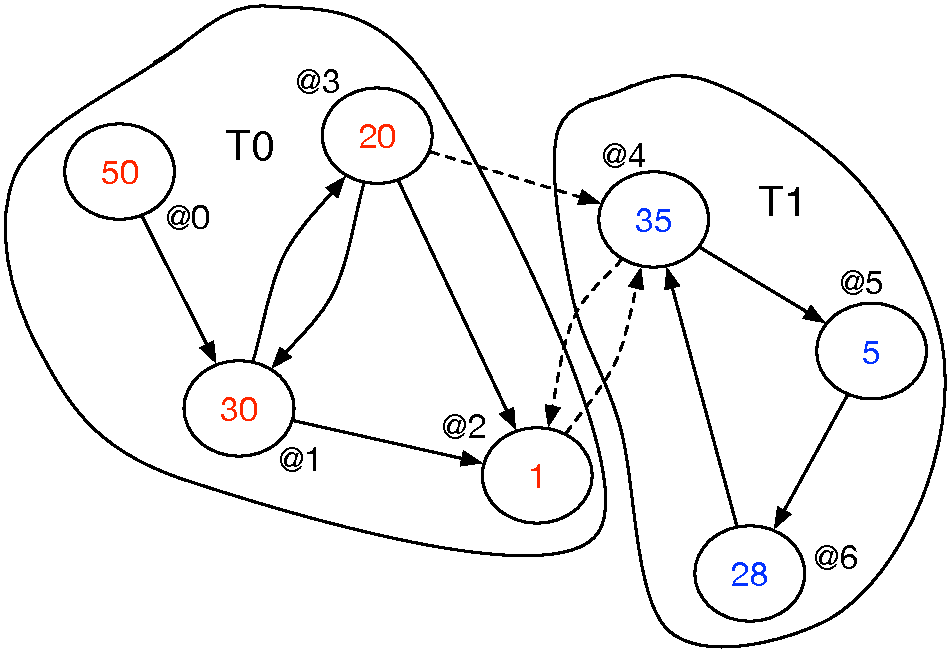
\includegraphics[width=0.7\textwidth]{figures/coordination/priorities.pdf}
\end{center}
\caption{Priorities with sub-graph partitioning. Priorities are used on a
   per-thread basis therefore thread \texttt{T0} schedules \texttt{@0} to
   execute, while \texttt{T1} schedules node \texttt{@4}.}
\label{fig:coordination:priorities}
\end{figure}


\section{Partitioning Facts}
We provide several coordination facts for dealing with node partitioning among
the running threads. Since each node is placed in some thread, the partitioning
facts revolve around thread placement.  In terms of action facts, we have the
following:

\begin{itemize}
   \item \code{set-thread(node A, thread T)}: Moves node \texttt{A} to thread
   \texttt{T}.

   \item \code{set-affinity(node A, node B)}: Places node \texttt{B} in
   the thread of node \texttt{A}.

   \item \code{set-static(node A)}: Forces node \texttt{A} to stay in the
   same thread indefinitely.

   \item \code{set-moving(node A)}: Allows node \texttt{A} to move freely
   between threads.

\end{itemize}

As an example of \texttt{set-thread}, consider again the graph in
Fig.~\ref{fig:coordination:priorities}. If a coordination fact
\texttt{set-thread(@2, T1)} is derived, then node \texttt{@2} will become part
of the sub-graph of thread \texttt{T1}. The result is shown in
Fig.~\ref{fig:coordination:partitioning}.

\begin{figure}
\begin{center}
   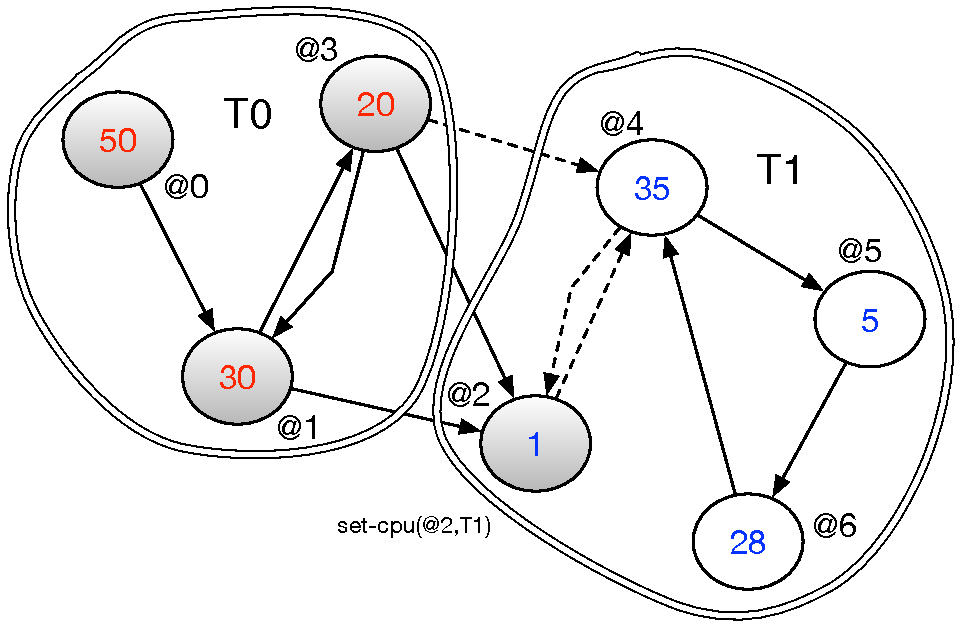
\includegraphics[width=0.6\textwidth]{figures/coordination/partitioning.pdf}
\end{center}
\caption{Moving node \texttt{@2} to thread \texttt{T1} using
   \texttt{set-thread(@2, T1)}.}
\label{fig:coordination:partitioning}
\end{figure}

Sensing facts retrieve information about node placement and are specified as
follows:

\begin{itemize}

   \item \code{thread-id(node A, thread T)}: Linear fact that maps node \code{A}
      to thread \code{T} which \code{A} belongs to. Fact \code{set-thread}
      implicitly updates fact \code{thread-id}.

   \item \code{is-static(node A)}: Fact available at node \texttt{A} if
   \item \code{is-moving(node A)}: Fact available at node \texttt{A} if
      \texttt{A} is allowed to move between threads.

      \texttt{A} is not allowed to move between threads.

   \item \code{just-moved(node A)}: Linear fact derived by the
      \code{set-thread} action if, at that moment, the node \code{A} is running
      on the target thread.

\end{itemize}



\section{Global Directives}

We also provide a few global coordination statements that cannot be specified
as sensing or action facts but are still important:

\begin{itemize}

   \item \texttt{priority @order ORDER} (\texttt{ORDER} can be either \code{asc}
      or \code{desc}): Defines if priorities are to be selected by the smallest
      or the greatest value, respectively.

   \item \texttt{priority @initial P}: Informs the runtime system that all nodes
   must start with temporary priority \code{P}. Alternatively, the programmer can define an
      \texttt{set-priority(A, P)} fact.

   \item \texttt{priority @default P}: Informs the runtime system that all nodes
      must start with default priority \code{P}. Alternatively, the programmer can define an
      \texttt{set-default-priority(A, P)} fact.

   \item \texttt{priority @base P}: Informs the runtime system that the
      \emph{base priority} should be \code{P}. The base priority is, by default,
      0 when the priority ordering is \code{asc} and $-\infty$ when the ordering
      is \code{desc}.

\end{itemize}

\section{Implementation}
In order to support priorities and node partitioning, we extended the work queue
of each thread, as presented in Fig.~\ref{fig:implementation:vm_overview}, to
include two new pairs of queues: two doubly linked lists known as the
\emph{standard queue} and two min/max heaps known as the \emph{priority queue}.
The standard queue contains nodes without priorities and supports push into
tail, remove node from the head, remove arbitrary node, and remove first half of
nodes.  The priority queue contains nodes with priorities and is implemented as
a binary heap array.  It supports the following operations: push into the heap,
remove the \emph{min} node, remove an arbitrary node, remove half of the nodes
(vertical split), and priority update.  Operations for removing half of the
queue are implemented in order to support node stealing, while operations to
remove arbitrary nodes or update priority allows threads to change the priority
of nodes.  Table~\ref{fig:implementation:table_queue} shows the complexity of
queue operations and compares the standard queue against the priority queue.
Except for the remove half operation, priority queue operations are more
expensive.

\begin{table}[h]
   \begin{tabular}{| c | c | c |}
      \hline
      \textbf{Operation} & \textbf{Standard queue} & \textbf{Priority Queue} \\
      \hline
      Push & $\mathcal{O}(1)$ & $\mathcal{O}(\log{N})$ \\ \hline
      Pop & $\mathcal{O}(1)$ & $\mathcal{O}(\log{N})$ \\ \hline
      Remove & $\mathcal{O}(1)$ & $\mathcal{O}(\log{N})$ \\ \hline
      Remove Half & $\mathcal{O}(N)$ & $\mathcal{O}(\log{N})$ \\ \hline
      Priority Update & - & $\mathcal{O}(\log{N})$ \\ \hline
   \end{tabular}
   \caption{Complexity of queue operations for both the standard
      queue and the priority queue.}
   \label{fig:implementation:table_queue}
\end{table}

\begin{figure*}[t]
\centering
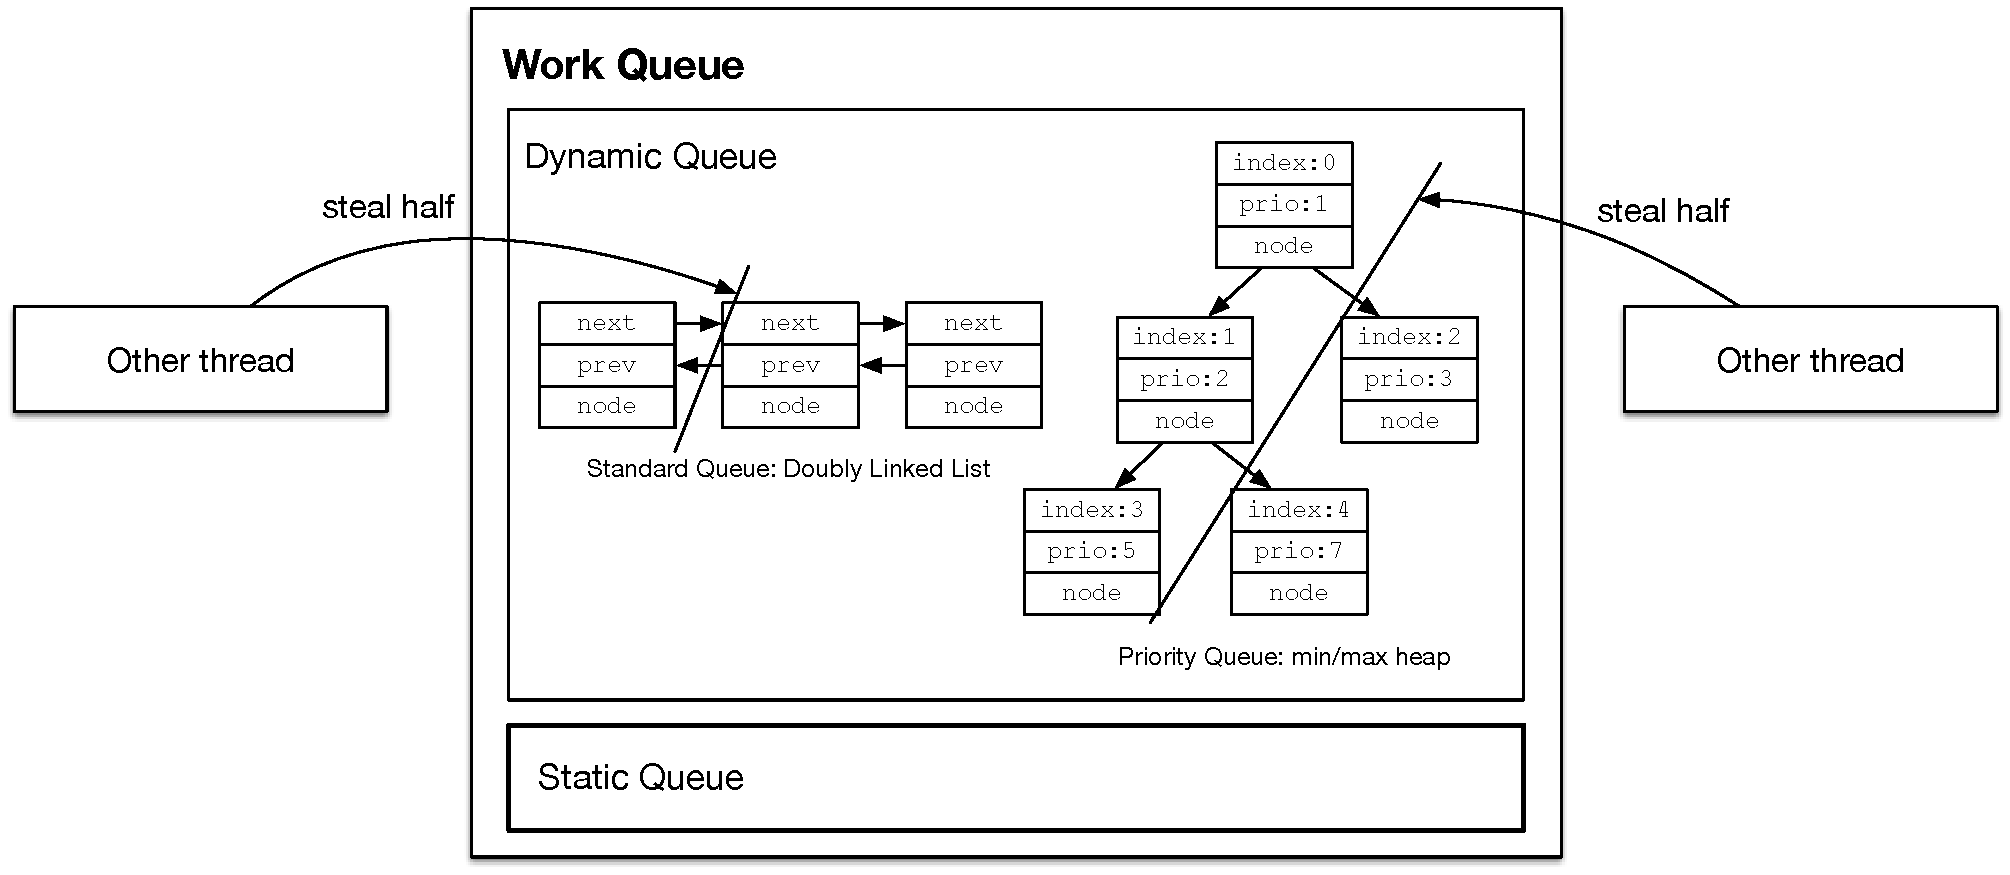
\includegraphics[width=0.95\textwidth]{figures/implementation/work_queue.pdf}
\caption{Thread's work queue and its interaction with other threads: the dynamic queue contains nodes that can be
   stolen while the static queue contains nodes that cannot be stolen. Both
   queues are implemented with one standard queue and one priority queue.}
\label{fig:implementation:work_queue}
\end{figure*}

The \texttt{next} and \texttt{prev} pointers of the standard queue are part of
the node structure in order to save space. These pointers are also used in the
priority queue but for storing the current priority and the index in the binary
heap array. Both the standard and priority queue are implemented as a pair of
queues. This first queue of each pair is a \emph{static queue} which contains
nodes that cannot be stolen and the second queue is the \emph{dynamic queue}
which contains nodes which can be stolen by other threads.
Figure~\ref{fig:implementation:work_queue} presents an overview of the two pairs
of queues and how the remove half operations are implemented in both queues in
order to support node stealing.  In the regular queue, the first $n/2$ elements
are removed from the front of the list and, in the priority queue, the binary
heap is split vertically for improved distribution of priorities.

Remember that to minimize inter-thread communication, node priorities are
implemented at the thread level, i.e., when a thread picks the highest priority
node from the priority queue, it picks the highest priority node from its
subgraph of nodes and not the highest priority node from the whole graph.

\subsection{Node State Machine}\label{sec:node_state_machine}

To accommodate the new coordination facilities, we added a new node state to the
state machine presented previously in Fig.~\ref{fig:local:node_states}.
Figure~\ref{fig:implementation:node_states} reviews the new set of states of
the state machine.

\begin{itemize}
   \item \textbf{running}: The node is deriving rules.
   \item \textbf{inactive}: The node is inactive, i.e., it has no new facts and
      it is not in any
   queue for processing.
   \item \textbf{active}: The node has new facts and it is in some queue waiting
   to be processed.
   \item \textbf{stealing}: The node has just been stolen and it is in the process of being
   moved to another thread.
   \item \textbf{coordinating}: The node moves from one queue to another or
      inside the priority queue when changing its priority.
\end{itemize}

\begin{figure}[ht]
   \centering
   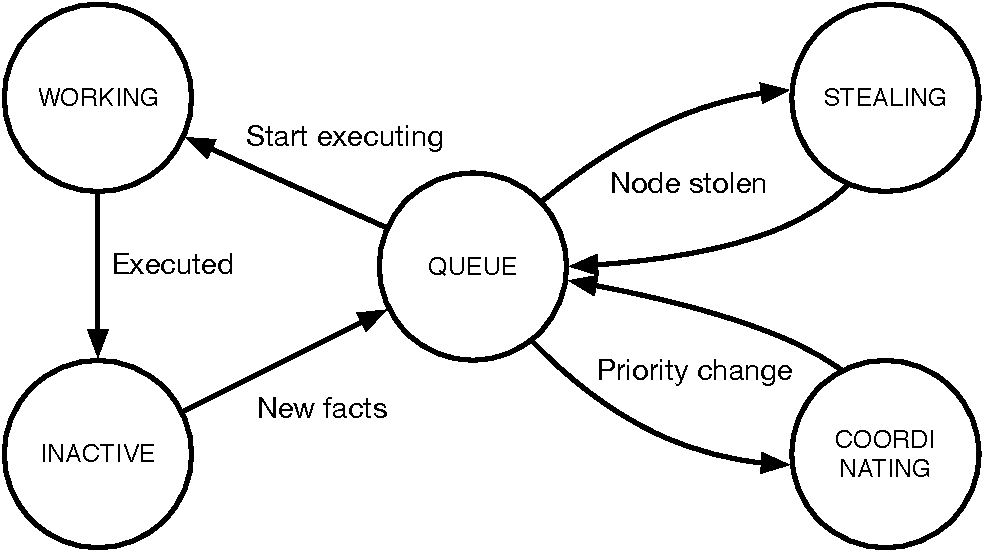
\includegraphics[width=0.55\textwidth]{figures/implementation/node_states.pdf}
   \caption{Node state machine extended with the new \textbf{coordinating}
   state.}
   \label{fig:implementation:node_states}
\end{figure}

\subsection{Coordination Instructions}\label{section:coordination:coord_instrs}

Coordination facts are implemented as API calls to the virtual machine which
implement the appropriate operations. Sensing facts read information about the
state of the virtual machine while action facts lock and update the appropriate
underlying data structures such as the node data structure or the thread's
queues.

When a thread $T_1$ performs coordination operations to a node owned by a thread
$T_2$, it needs to synchronize with $T_2$ and for that the \emph{State Lock} in
the target node needs to be acquired. Optionally, we may need to also lock the
queues of the thread $T_2$ if the priority is being updated or the queues of
thread $T_1$, if the node is moving to thread $T_1$. Note that both the standard
queue and priority queue have separate locks in order to allow concurrent
manipulation of the two data structures.

For the coordination facts \code{set-priority} and \code{add-priority}, when
multiple operations are directed to the same node during a single node
execution, we coalesce the multiple operations into a single operation.  As an
example, if a node derives two \code{set-priority} facts that change the
priority of node \code{@1} to \code{1} and \code{2}, the virtual machine
coalesces the two instructions into a single \code{set-priority} that is applied
with value \code{2} (the higher priority) after all the candidate rules of the
node are executed. The reason for this optimization is that nodes may run for
some number of steps during the lifetime of the program, therefore immediately
applying each and every coordination instruction is not cost effective. We aim
to reduce the amount of locking and movement of nodes inside the queues due to
priority updates.


\section{Coordinating SSSP}
Now that we have presented the coordination facts for LM, we are now in a
position to use them in the SSSP program presented before.  The coordinated
version of the SSSP~(Fig.~\ref{code:shortest_path_program_coord}) uses the
coordination fact \texttt{set-priority} (line 14) and a global program directive
to order priorities in ascending order (line 5).

When run with one thread, the algorithm behaves like Dijkstra's shortest path
algorithm~\cite{Dijkstra}. When using multiple threads, each thread will pick
the shortest distance from their subset of nodes.  While this does not yield the
optimal program with relation to 1 thread, it allows for parallel execution and
locally avoids unnecessary work. The result scales well and it is close to
Dijkstra's algorithm.

\begin{figure}[ht]
\begin{Verbatim}[numbers=left,xleftmargin=7mm,commandchars=\\\{\}]
type route edge(node, node, int).
type linear shortest(node, int, list int).
type linear relax(node, int, list int).

\underline{priority @order asc}.

shortest(A, +00, []).
relax(@1, 0, [@1]).

shortest(A, D1, P1), D1 > D2, relax(A, D2, P2)
   -o shortest(A, D2, P2),
      \{B, W | !edge(A, B, W) |
         relax(B, D2 + W, P2 ++ [B]),
         \underline{set-priority(B, float(D2 + W))}\}.

shortest(A, D1, P1), D1 <= D2, relax(A, D2, P2)
   -o shortest(A, D1, P1).
\end{Verbatim}
   \caption{Shortest Path Program coordinated with \texttt{set-priority}.}
   \label{code:shortest_path_program_coord}
\end{figure}

The most interesting property of the SSSP program presented in
Fig.~\ref{code:shortest_path_program_coord} is that it remains provably correct,
although it applies rules using smarter ordering and the code remains
declarative. Since the proof of correctness considers that, eventually, the
shortest path is computed at all nodes of the graph, the use of
\texttt{set-priority} does not change this at all.


\section{Applications}

To further understand how coordination facts work, we present other programs that
take advantage of them.

\subsection{Belief Propagation}

Randomized and approximation algorithms can obtain significant benefits from
coordination directives because although the final program results will not be
exact, they follow important statistical properties and can be computed faster.
An examples of such programs is PageRank~\cite{Lubachevsky:1986:CAA:4904.4801}
and Loopy Belief Propagation~\cite{Gonzalez+al:aistats09paraml}, which is the
focus of this section.

Loopy Belief Propagation (LBP) is an approximate inference algorithm used in
graphical models with cycles~\cite{Murphy99loopybelief}. In its essence, LBP is
a sum-product message passing algorithm where nodes exchange messages with their
immediate neighbors and apply some computations to the messages received.

LBP is an algorithm that maps very well to the graph-based model of LM. The
original algorithm computes the belief of all nodes for several iterations with
synchronization between iterations. However, it is possible to avoid the
synchronization step, if we take advantage of the fact that LBP will converge
even when using an asynchronous approach. So, instead of computing the belief
iteratively, we keep track of all messages sent/received (and overwrite them
when we receive a new one) and recompute the belief asynchronously.
Figure~\ref{fig:coordination:bp} shows the communication patterns for our
application and Fig.~\ref{code:coordination:bp} presents the LM code for the
implementation.

\begin{figure}[h]
   \begin{center}
      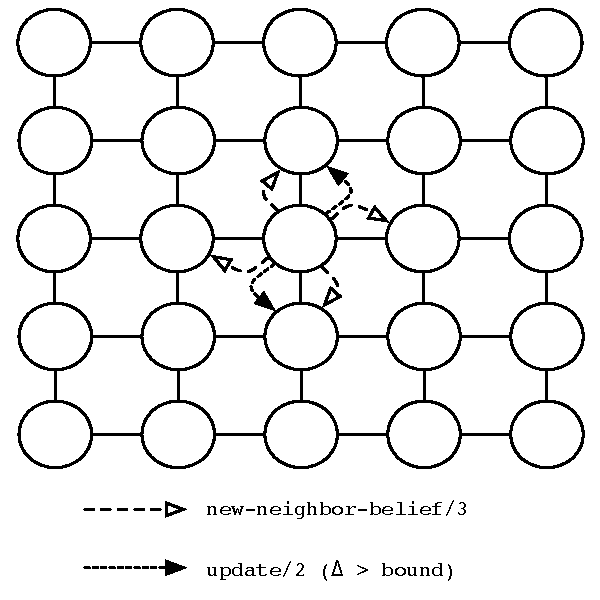
\includegraphics[width=0.3\textwidth]{figures/bp/bp.pdf}
   \end{center}
\caption{LBP: communication patterns}
\label{fig:coordination:bp}
\end{figure}

\begin{figure}[h!]
   \begin{Verbatim}[numbers=left, fontsize=\scriptsize]
neighbor-belief(A, B, Belief),
new-neighbor-belief(A, B, NewBelief)
   -o neighbor-belief(A, B, NewBelief).

check-residual(A, Residual, B),
Residual > bound
   -o update(B).
check-residual(A, _, _) -o 1.

// update belief to be sent to one neighbor
update-messages(A, NewBelief),
!edge(A, B),
neighbor-belief-old(A, B, OldIn),
sent-neighbor-belief(A, B, OldOut),
Cavity = normalize(divide(NewBelief, OldIn)),
Convolved = normalize(convolve(global-potential, Cavity)),
OutMessage = damp(Convolved, OldOut, damping)
   -o Residual = residual(OutMessage, OldOut),
      check-residual(A, Residual, B),
      update-messages(A, NewBelief),
      new-neighbor-belief(B, A, OutMessage),
      sent-neighbor-belief(A, B, OutMessage).

update-messages(A, NewBelief) -o 1.

// if we have two update functions, just run one of them
update(A), update(A) -o update(A).

// make a copy of neighbors beliefs in order to add them up
update(A),
!potential(A, Potential),
belief(A, MyBelief)
   -o [custom addfloats Potential => Belief | B, Belief |
         neighbor-belief(A, B, Belief) |
         neighbor-belief-old(A, B, Belief), neighbor-belief(A, B, Belief) |
         Normalized = normalizestruct(Belief),
         update-messages(A, Normalized), belief(A, Normalized)].
\end{Verbatim}
\caption{LM code for the Loopy Belief Propagation problem.}
\label{code:coordination:bp}
\end{figure}

Belief values are arrays of floats and are represented by \texttt{belief/2}
facts. The first rule (lines 1-3) updates a given neighbor belief whenever a new
belief value is received. This is the highest priority rule since we want to
update the neighbor beliefs before doing anything else. In order to store the
belief values of the neighbor nodes, we use \texttt{neighbor-belief/3} facts,
where the second argument is the neighbor address and the third argument is the
belief value.

The last two rules (lines 26-37) update the belief value of a node. An
\texttt{update/1} fact starts the process. The first rule (lines 27) simply
consumes redundant \texttt{update/1} facts and the second rule (lines 30-37)
performs the belief update by aggregating all the neighbor belief values. The
aggregate in lines 33-37 also derives copies of the neighbors beliefs that need
to be consumed in order to compute the belief value that is going to be sent to
the target neighbor. The aggregate uses a custom accumulator that takes two
arrays and adds the floating point numbers at each index of the array.  The rule
in lines 10-22 iterates through the neighbor belief values and sends new belief
values by performing the appropriate computations on the new belief value of the
current node and on the belief value sent previously.  Once the facts
\texttt{neighbor-belief-old} are fully consumed, the rule in line 24 is fired in
order to consume \texttt{update-messages}.

For each neighbor update, we also check in lines 5-8 if the change in belief
values is greater than \texttt{bound} (a program constant) and then force the
neighbor nodes to update their belief values by deriving \texttt{update(B)}.
This allows neighbor nodes to use updated neighbor values and recompute their
own belief values using better information. The computation of belief values
will then start to converge to their true belief values, independently of the
node scheduling used. However, if we prioritize nodes that receive new neighbor
belief values with a larger \texttt{Residual} then we will converge faster.
Figure~\ref{code:coordination:improved_bp} shows the fourth rule modified with
\texttt{add-priority} in order to increase to priority of neighbor nodes when
the source node has large changes in its belief value.

\begin{figure}[h!]
\begin{Verbatim}[numbers=left,commandchars=\\\{\},fontsize=\scriptsize]
// update belief to be sent to one neighbor
update-messages(A, NewBelief),
!edge(A, B),
neighbor-belief-old(A, B, OldIn),
sent-neighbor-belief(A, B, OldOut),
Cavity = normalize(divide(NewBelief, OldIn)),
Convolved = normalize(convolve(global-potential, Cavity)),
OutMessage = damp(Convolved, OldOut, damping)
   -o Residual = residual(OutMessage, OldOut),
      \underline{add-priority(B, Residual)},
      check-residual(A, Residual, B),
      update-messages(A, NewBelief),
      new-neighbor-belief(B, A, OutMessage),
      sent-neighbor-belief(A, B, OutMessage).
\end{Verbatim}
\caption{Updating the BP program to use priorities.}
\label{code:coordination:improved_bp}
\end{figure}


\section{Related Work}

As mentioned in Section~\ref{sec:background:coordination}, Linda~\cite{linda}
and Delirium~\cite{Delirium} are two programming languages that support
coordination. When compared to LM, Linda and Delirium are limited in the sense
that the programmer can only coordinate the scheduling of processing units,
while placement of data is left to the implementation. LM differs from those
languages because coordination acts on data instead of processing units.
Coordination facts as used in this chapter raise the abstraction by considering
data and algorithmic aspects of the program instead of focusing on how
processing units are used. Furthermore, LM is both a coordination language and a
computation language and the distinction between the two components is small.

There are also several programming models also support some kind of coordination
primitives that allow explicit scheduling and load balancing of work between
available processing units but are not considered proper programming languages.

The Galois~\cite{Pingali:2011:TPA:1993316.1993501} programming model implements
autonomous scheduling by default, where activities may be rolled back in case of
conflict. However, it is possible to employ a concrete scheduling strategy for
coordinating parallel execution in order to improve execution and avoid
conflicts.  First, there is \emph{compile-time coordination}, where the
scheduling ordered is computed during compilation and is pre-defined before the
program is executed. Secondly, there is \emph{runtime coordination}, where the
order of activities is computed during execution. The execution of the algorithm
proceeds in rounds: first, a set of non-conflicting activities is computed and
then executed by applying the operator; conflicting activities are postponed to
the next round. The third and last scheduling strategy is \emph{just-in-time
coordination} where the order of activities is defined by the underlying data
structure where the operator is applied (for instance, computing on a graph
may depend on its topology).

In the context of the Galois model, Nguyen et al.~\cite{nguyen11} expanded the
concept of runtime coordination with the introduction of a flexible approach to specify
scheduling policies for Galois programs. This approach was motivated by the fact
that some algorithms can be executed faster if computations use better
scheduling strategies. The scheduling language specifies 3 main scheduler types:
FIFO (First-In First-Out), LIFO (Last-In First-Out) and
OrderedByMetric (order activities by some metric). These schedulers can
be composed and synthesized without requiring users to write complex concurrent
code.

Elixir~\cite{Prountzos:2012:ESS:2384616.2384644} is a domain specific language
that builds on top of the Galois and allows easy specification of scheduling
strategies.  The main idea behind Elixir is that the user should be able to
specify how operator application is scheduled and the framework will compile
this high level specification to low level code using the provided scheduling
specification. One of the motivating examples is the Single Source Shortest Path
program that can be specified using multiple scheduling specifications,
generating different well-known shortest path algorithms such as the
Dijkstra or Bellman-Ford algorithm. Unlike the work of Nguyen et
all.~\cite{nguyen11}, Elixir does not allow graph mutations.

Halide~\cite{Ragan-Kelley:2013:HLC:2491956.2462176} is a language and compiler
for image processing pipelines with the goal of optimizing parallelism, locality
and re-computation. Halide decouples the algorithm definition from its execution
strategy, allowing the compiler to find which execution strategy may be the best
for optimizing for locality and parallelism. The language allows the programmer
to specify the scheduling strategy, allowing the programmer to decide the order
of computations, what intermediate results need to be stored, how to split the
data among processing units and how to use vectorization and the well-known
sliding window mechanism. However, the compiler is able to use stochastic search
to find good schedules for Halide pipelines. Notably, experimental results
indicate that automatic search sometimes leads to better execution than
hand-written code.

In contrast to the previous systems, LM stands alone in making coordination
(both scheduling and partitioning) a first-class programming construct and
semantically equivalent to computation. Furthermore, LM distinguishes itself by
supporting data-driven dynamic coordination, particularly for irregular data
structures. Elixir and Galois do not support coordination for data partitioning,
and, in Elixir, the coordination specification is separated from computation,
limiting the programmability of coordination. Compared to LM, Halide is
targeted for regular applications and therefore only supports compile time
coordination.

\section{Chapter Summary}

In this chapter, we presented the current set of coordination directives,
implemented as sensing and action facts. The use of such facilities allows the
programmer to write derivation rules that change how the runtime system
schedules computation thus improving the executing time and possibly the final
program results. In terms of programming language design, our coordination
mechanisms are unique in the sense that they are treated like regular
computation, which allows for complex run-time coordination policies and can be
made part of the main program's logic.


\chapter{Thread-Based Facts: Exploring Explicit Parallelism}
In the previous chapter, we introduced coordination facts, a mechanism that can
be used by the programmer to coordinate execution. While these facilities retain
the implicit parallelism of the language, they do not allow the programmer to
fully reason about the underlying parallel architecture since the only reasoning
allowed relates to node partitioning and data placement. In principle, it should
be advantageous to reason about thread state, that is, to perform rule inference
about facts stored on each thread and allow threads to communicate and
coordinate between them depending on their current state. This introduces a kind
of explicit parallelism into the implicit parallel model of LM.  However, this
explicit parallelism remains declarative so that the programmer is able to
reason thread coordination as well as it does with regular computation.

\section{Motivational Example: Graph Searching}
Consider the problem of checking if a set of nodes $S$ in a graph $G$ is
reachable from an arbitrary node $N$. An obvious solution to this problem is to
start at $N$, gather all the neighbor nodes into a list and then recursively
visit all those reachable nodes, until $S$ is covered. This reduces to a problem
of performing a breadth or depth-first search on graph $G$. However, this
solution is sequential and does not have much concurrency.  An alternative
solution to the problem is to recursively propagate the search to all neighbors
and aggregate the results in the node where the search started.  The code for
this later solution is shown in Fig.~\ref{code:threads:reach_simple}.

\begin{figure}[h]
\begin{Verbatim}[numbers=left,fontsize=\codesize,commandchars=*\#\&]
type int id.*hfill// Type declaration
type list int reach-list.

type edge(node, node).*hfill// Predicate declaration
type value(node, int).
type linear search(node, id, reach-list).
type linear do-search(node, id, node, reach-list).
type linear lookup(node, id, reach-list, int Val).
type linear new-lookup(node, id, int Val).
type linear visited(node, id).

search(A, Id, ToReach)*label#line:threads:reach_lookup1&*hfill// Rule 1: initialize search
   -o do-search(A, Id, A, ToReach),
      lookup(A, Id, ToReach, []).*label#line:threads:reach_lookup2&

lookup(A, Id, ToReach, Found), new-lookup(A, Id, Val)*hfill// Rule 2: new reachable node found
   -o lookup(A, Id, remove(ToReach, Val), [Val | Found]).

do-search(A, Id, Node, ToReach),*label#line:threads:reach_visit1&*hfill// Rule 3: node has already seen this search
visited(A, Id)
   -o visited(A, Id). *label#line:threads:reach_visit2&

do-search(A, Id, Node, ToReach),*hfill// Rule 4: node found and propagate search
!value(A, Val), Val in ToReach*hfill// New node was found.
   -o visited(A, Id),*label#line:threads:reach_visit_visited1&
      new-lookup(Node, Id, Val),
      {B | !edge(A, B) -o do-search(B, Id, Node, remove(ToReach, Val))}.*label#line:threads:reach_propagate&

do-search(A, Id, Node, ToReach),*hfill// Rule 5: node not found and propagate search
!value(A, Val), ~ Val in ToReach*hfill// Not the node we are looking for.
   -o {B | !edge(A, B) -o do-search(B, ID, Node, ToReach)},*label#line:threads:reach_propagate2&
      visited(A, Id).*label#line:threads:reach_visit_visited2&
\end{Verbatim}

\caption{LM code to perform reachability checking on a graph.}
\label{code:threads:reach_simple}
\end{figure}

Each distinct reachability search is represented by a number (\code{Id}) and a
\code{search} axiom. Associated to each search \code{Id} is a list of nodes to
reach.  The predicate \code{visited} marks nodes that have already
participated in search, while predicate \code{do-search} is used to propagate a
specific search. The first rule
(lines~\ref{line:threads:reach_lookup1}-\ref{line:threads:reach_lookup2}) starts
a particular search by deriving a \code{do-search} and an \code{lookup} fact.
The \code{lookup} fact is used as an accumulator and is stored in the starting
node. The third rule
(lines~\ref{line:threads:reach_visit1}-\ref{line:threads:reach_visit2}) avoids
visiting the same node twice in the presence of a \code{visited} fact.  This
visited fact is derived in the next two rules
(lines~\ref{line:threads:reach_visit_visited1}
and~\ref{line:threads:reach_visit_visited2}).  If the node where the search is
being performed is in the set of nodes we want to reach (\code{ToReach}) then we
remove the node value from the list and propagate the search to the neighbor
nodes (line~\ref{line:threads:reach_propagate}).  Otherwise, the search is
propagated but no value is removed from \code{ToReach}.

As an example, consider Fig.~\ref{fig:threads:reach_example}, which shows 2
reachability checks on a graph with 10 nodes. For instance, the search with
\code{Id = 0} starts at node \code{@1} and checks if nodes \code{@1}, \code{@2},
and \code{@3} are reachable from \code{@1}. Since \code{@1} is the starting
node, \code{1} is immediately removed from the reachable list, including the
propagated \code{do-search} facts but also the \code{lookup} fact that is stored
at node \code{@1}. Once \code{do-search} reaches node \code{@3}, the value
\code{3} is removed from the list and a new \code{do-search} is propagated to
node \code{@1} (not shown in the figure) and \code{@2}. At the same time, node
\code{@2} receives the list \code{[2,3]}, removes \code{2} and propagates
\code{[3]} to node \code{@3} and \code{@1}. Node \code{@1} receives two
\code{new-lookup} facts, one from \code{@3} and another from \code{@2}, due to
successful searches and the \code{lookup} fact becomes \code{lookup(@1,0,[],
[1,2,3])}.

The attentive reader will notice that node \code{@1} already knows that all the
nodes have been reached and that nodes \code{@7} and \code{@4} will, needlessly,
continue to check if \code{[2,3]} are reachable. This is an issue that arises
because the programmer has valued concurrency by increasing redundancy and
reducing communication between nodes. It would be prohibitly expensive to share
reachability information between nodes. An alternative solution is to store the
results of the search on the thread performing the search and then coordinate
the results with other threads since the number of threads is usually smaller
than the number of nodes. Before showing how the reachability program is solved
using thread-based facts, we first present the changes to the language.

\begin{figure}[ht]
\begin{center}
   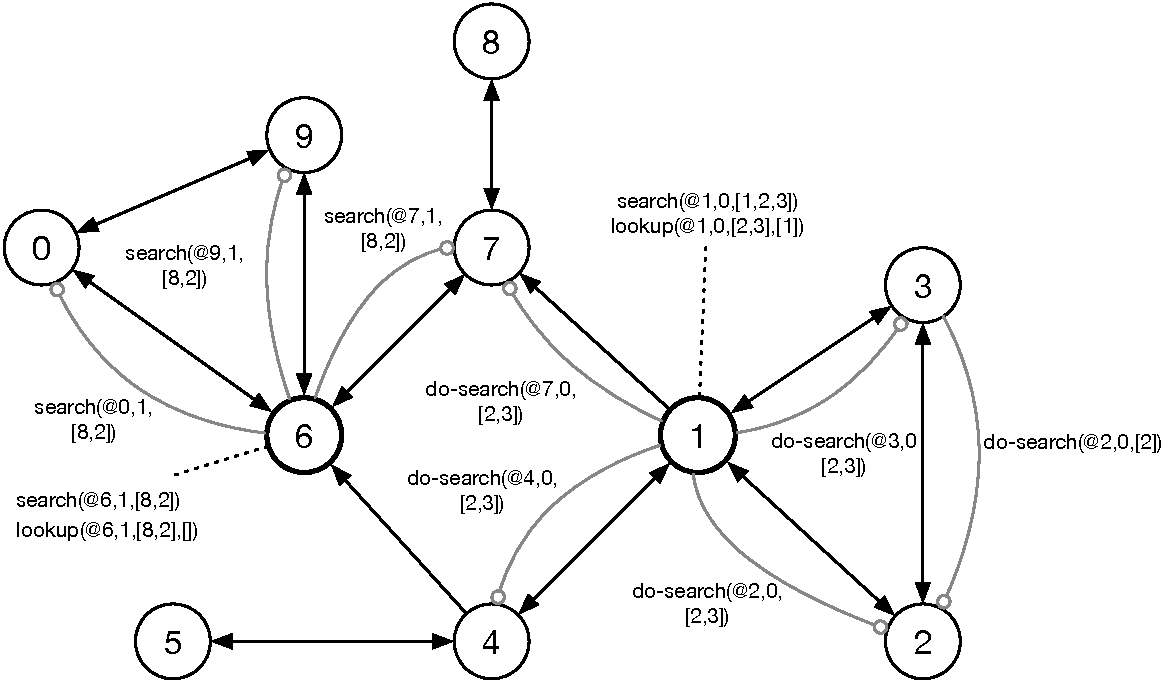
\includegraphics[width=0.9\linewidth]{figures/threads/reach.pdf}
\end{center}

\caption{Performing reachability checks on a graph using nodes \code{@1}
(\code{Id = 0}) and \code{@6} (\code{Id = 1}).  Search with \code{Id = 0} wants
to reach nodes \code{@1}, \code{@2}, and \code{@3} from node \code{@1}. Since
\code{@1} is part of the target nodes, the fact \code{do-search} propagated to
neighbor nodes does not include \code{1}.}

\label{fig:threads:reach_example}
\end{figure}

\subsection{Language Changes}

In the previous chapter, we presented coordination facts such as
\code{thread-id} and \code{set-thread} that already bring some awareness about
the underlying parallel system. Furthermore, such facts also introduce the
\code{thread} type for predicate arguments, which refers to a thread in the
system that is related to a core in a multi core processor. We now introduce the
concept of \emph{thread facts}, which are logical facts stored at the thread
level, meaning that, each thread is now an entity with its own logical facts.
The type \code{thread} is also now the type of the first argument of
\emph{thread predicates}, indicating that the predicate is related and is to be
stored in a specific thread. We also view the available threads as forming a
separate graph from the data graph, a graph of the processing units which are
operating on the data graph.

The introduction of thread facts increases the expressiveness of the system in
the sense that it is now possible to write inference rules that reason about the
state of the threads. This creates optimization opportunies since we can now
write algorithms with global information stored in the thread, while keeping the
LM language fully declarative. Moreover, threads are now allowed to explicitly
communicate with each other, and in conjunction with coordination predicates,
enable the writing of complex scheduling policies.

We discriminate between two new types of inference rules. The first type is the
\emph{thread rule} and has the form \code{a(T), b(T) -o c(T)}, and can be read
as: if thread \code{T} has fact \code{a(T)} and \code{b(T)} then derive fact
\code{c(T)}. The second type is the \emph{mixed rule} and has the form
\code{a(T), d(N) -o e(N)} and can be read as: if thread \code{T} is executing
node \code{N} and has the fact \code{a(T)} and node \code{N} has the fact
\code{d(N)} then derive \code{e(N)} at node \code{N}. Thread rules reason solely
at the thread level, while mixed rules allow reasoning about both thread and
node facts. Logically, the mixed rule uses an extra fact \code{running(T, N)},
which indicates that thread \code{T} is currently executing node \code{N}. The
\code{running} fact is implicitly retracted and asserted every time the thread
selects a different node for execution. This makes our implementation efficient
since a thread does not need to look for nodes that match mixed rules and it is
then the scheduling of the program that drives the matching of such rules.

\subsection{Graph Of Threads}

Figure~\ref{fig:coord:thread_facts} represents a schematic view of the two graph
data structures of a program with three threads: thread $T1$ is executing node
\code{@5}, $T2$ is executing node \code{@4}, and $T3$ is executing node
\code{@3}. Note that every thread has access to its own facts and to the node
facts.

\begin{figure}[ht]
   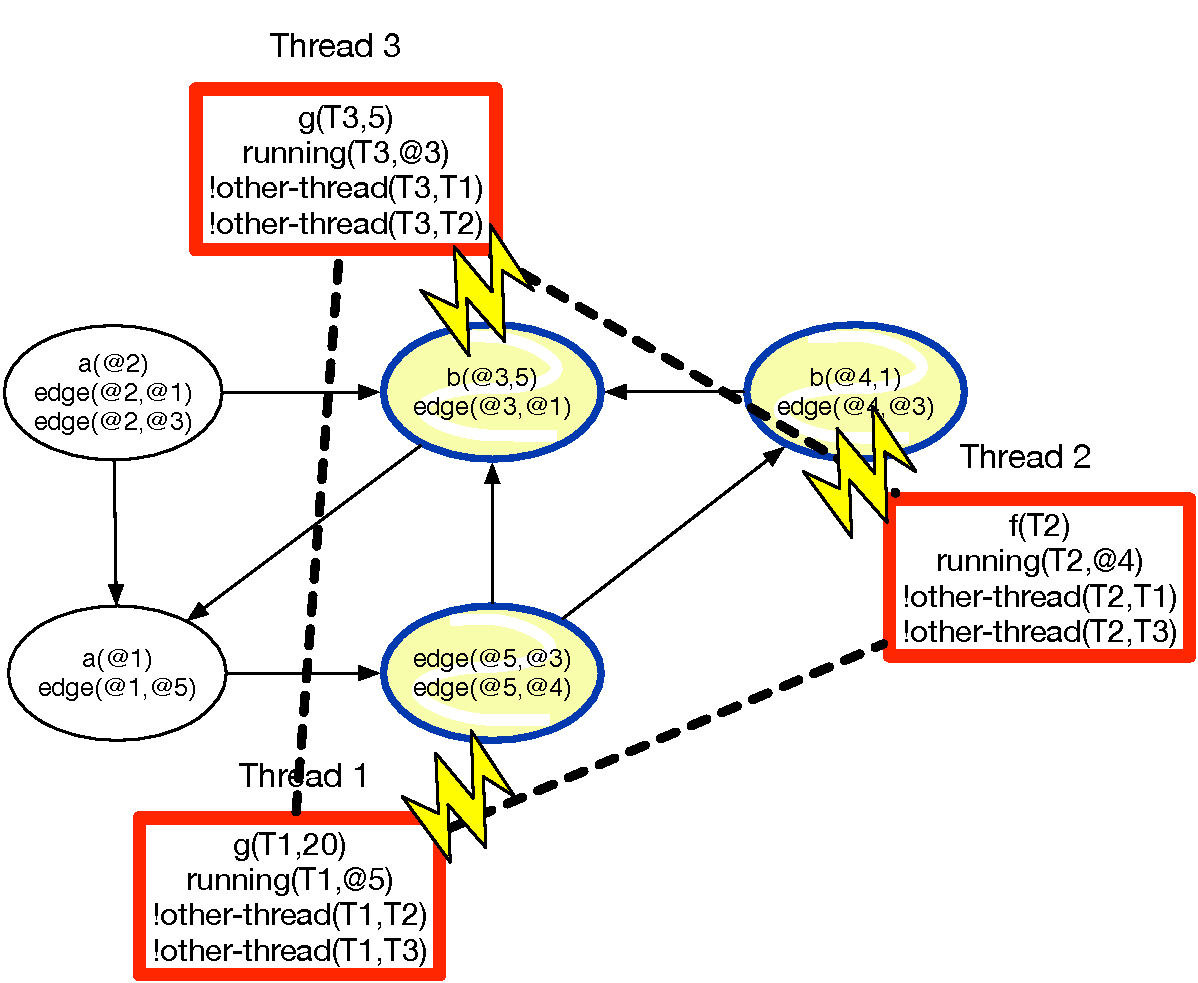
\includegraphics[width=0.6\linewidth]{figures/threads/threads.pdf}

   \caption{An example program being executed with three threads. Note that each
      threads has a \code{running} fact that stores the node currently being
   executed.}

   \label{fig:coord:thread_facts}
\end{figure}

We added several helpful predicates that allow the programmer to inspect the
graph of threads and reason about the state of computation as it relates to
threads:

\begin{itemize}
   \item \code{\bang thread-list(T, L)}: Fact instantiated in all threads where
      \code{L} is a list of all threads executing in the system.

   \item \code{\bang other-thread(T1, T2)}: Connects thread \code{T1} to all the
      other threads \code{T2} executing in the system. Note that in
      Fig.~\ref{fig:coord:thread_facts}, we use \code{\bang other-thread} fact
      to specify the graph of threads.


   \item \code{\bang leader-thread(T, TLeader)}: Fact instantiated in all
      threads where \code{TLeader} refers to a selected thread (the first thread
      in \code{L} of \code{\bang thread-list(T, L)}).

   \item \code{running(T, A)}: Used to retrieve the current node \code{A}
      running on thread \code{T}.
\end{itemize}

With the exception of \code{running}, every other fact is added at the beginning
of the program as a persistent fact.

\subsection{Reachability With Thread Facts}

We know update the graph reachability program presented in
Fig.~\ref{code:threads:reach_simple} to use thread facts in order to avoid
needless searches on the graph. The search process is still done concurrently as
before, but the search state is now stored in each thread, allowing the thread
to store partial results and coordinate with other threads. The code for this new
version is shown in Fig.~\ref{code:threads:reach_threads}.

Lines~\ref{line:threads:reacht_start1}-\ref{line:threads:reacht_start2} start
the search process by assigning a thread \code{Owner} to search \code{Id} using
the persistent fact \code{\bang thread-list} which contains the list of all
available threads in the system. Next, in
line~\ref{line:threads:reacht_threads}, a fact \code{thread-search} is created
for all threads using a comprehension. We use predicate \code{do-search} to
propagate the search through the graph and a predicate \code{visited} to mark
nodes already processed for a specific search.  The two rules in
lines~\ref{line:threads:reacht_check1}-\ref{line:threads:reacht_check2}
propagate the search process to the neighbor nodes and check if the current node
is part of the list of nodes we want to reach.

An interesting property of this version is that each owner thread responsible
for a search keeps track of the remaining nodes that need to be reached. In
line~\ref{line:threads:reacht_remove}, we derive \code{remove-thread-search} in
order to inform owner threads about new reachable nodes. Once an owner thread
detects that all nodes have been reached (lines
\ref{line:threads:reacht_reached1}-\ref{line:threads:reacht_reached2}), all the
other threads will know that and update their search state accordingly
(lines~\ref{line:threads:reacht_knows1}-\ref{line:threads:reacht_knows2}). When
every thread knows that all nodes were reached, they will consume
\code{do-search} facts (lines
\ref{line:threads:reacht_prune1}-\ref{line:threads:reacht_prune2}), effectively
pruning the search space.

\begin{figure}[h]
\begin{Verbatim}[numbers=left,fontsize=\codesize,commandchars=*\#\&]
search(A, Id, ToReach),*label#line:threads:reacht_start1&*hfill// Rule 1: initialize search
*textbf#!thread-list(T, L)&, Owner = nth(L, Id % @threads)*hfill// Allocate search to a thread
   -o {T2 | *textbf#!other-thread(T, T2)& -o *textbf#thread-search(T2, Id, ToReach, Owner)&},*label#line:threads:reacht_threads&
      do-search(A, Id).*label#line:threads:reacht_start2&

*textbf#thread-search(T, Id, [], Owner)&, *label#line:threads:reacht_prune1&*hfill// Rule 2: search completed
do-search(A, Id)
   -o *textbf#thread-search(T, Id, [], Owner)&. *label#line:threads:reacht_prune2&

do-search(A, Id),*hfill// Rule 3: node already visited
visited(A, Id)
   -o visited(A, Id).

do-search(A, Id),*label#line:threads:reacht_check1&*label#line:bfs_join1&*hfill// Rule 4: node found
*textbf#thread-search(T, Id, ToReach, Owner)&,*label#line:threads:reacht_join2&
!value(A, Val), Val in ToReach
   -o *textbf#thread-search(T, Id, remove(ToReach, Val), Owner)&,
      *textbf#remove-thread-search(Owner, Id, Val)&,*hfill// Tell owner thread about it.*label#line:threads:reacht_remove&
      {B | !edge(A, B) -o do-search(B, Id)},
      visited(A, Id).

do-search(A, Id),*hfill// Rule 5: node not found but propagate search
*textbf#thread-search(T, Id, ToReach, Owner)&,
!value(A, Val), ~ Val in ToReach
   -o *textbf#thread-search(T, Id, ToReach, Owner)&,
      visited(A, Id),
      {B | !edge(A, B) -o do-search(B, Id)}.*label#line:threads:reacht_check2&

*textbf#remove-thread-search(T, Id, Val), thread-search(T, Id, ToReach, Owner)&*hfill// Rule 6: node found
   *textbf#-o thread-search(T, Id, remove(ToReach, Val), Owner),&
      *textbf#check-results(T, Id).&

*textbf#check-results(T, Id),&*label#line:threads:reacht_reached1&*hfill// Rule 7: search is completed
*textbf#thread-search(T, Id, [], Owner)&
   *textbf#-o thread-search(A, Id, [], Owner),&
      *textbf#{B | !other-thread(T, B) -o signal-thread(B, Id)}.&*label#line:threads:reacht_reached2&

 *textbf#check-results(T, Id),&*hfill// Rule 8: search not completed yet
 *textbf#thread-search(T, Id, ToReach, Owner), ToReach <> []&
   *textbf#-o thread-search(T, Id, ToReach, Owner).&

*textbf#signal-thread(T, Id),&*hfill// Rule 9: thread knows search is done*label#line:threads:reacht_knows1&
*textbf#thread-search(T, Id, ToReach, Owner)&
   *textbf#-o thread-search(T, Id, [], Owner).& *label#line:threads:reacht_knows2&
\end{Verbatim}
\caption{Coordinated version of the reachability checking program. Note
that \code{@threads} represent the number of threads in the system.}
\label{code:threads:reach_threads}
\end{figure}

An alternative implementation could force every thread to share its reached
nodes to all the other threads in the system. However, this would generate a lot
of traffic between threads, which would actually make the program perform worse.
Our final solution is a good trade off since it only forces threads to
coordinate when pruning can actually happen.

Figure~\ref{fig:threads:results_search} presents experimental results of the
graph reachability program using 4 different datasets. Except for Random, all
the datasets were already used in the MSSD program and were presented before.
The Random dataset is a randomly generated graph with 50000 nodes and about a
million edges.  In the plots, we show the run time of the version without thread
facts (\textbf{Regular}) and the version using thread facts called
\textbf{Threads}. We also show the speedup of the \textbf{Threads} and
\textbf{Regular} versions against the \textbf{Regular} version with 1 thread.

Our results indicate that using thread facts produces a significant reduction in
run time. This is especially true in the case of datasets with large number of
edges, since less facts are produced and propagated in the graph when the
threads know that the search has been completed. The results also show that, in
the case of the Facebook dataset, in which the number of queries is the same as
the number of nodes, the use of thread facts does not produce great improvements
due to the costs of managing the reachability results on each thread's database.
These costs are related to the need to index and lookup \code{thread-search}
facts on the \code{Id} argument every time a node is inspected.

\begin{figure}[]
        \centering
        \begin{subfigure}[b]{\plotsize\textwidth}
           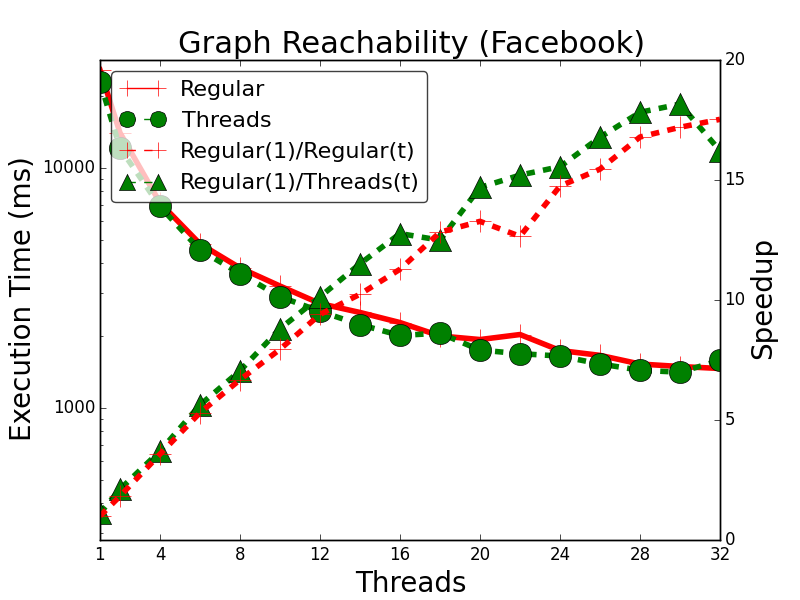
\includegraphics[width=\textwidth]{experiments/threads/cmp-search-facebook.png}
           \caption{Facebook has 2000 nodes and 20000 edges. The dataset makes
           2000 graph queries to 5\% of the graph's nodes.}
           \label{fig:threads:search_facebook}
        \end{subfigure}
        \spacing
        \begin{subfigure}[b]{\plotsize\textwidth}
           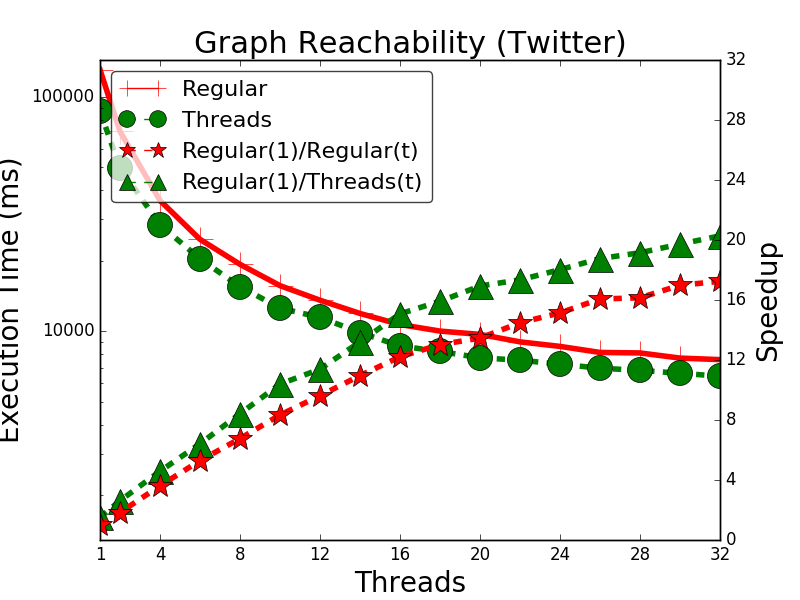
\includegraphics[width=\textwidth]{experiments/threads/cmp-search-twitter.png}
           \caption{Twitter has 81306 nodes and 1768149 edges. The dataset makes
           100 graph queries to 1\% of the graph's nodes.}
           \label{fig:threads:search_twitter}
        \end{subfigure} \\
        \begin{subfigure}[b]{\plotsize\textwidth}
           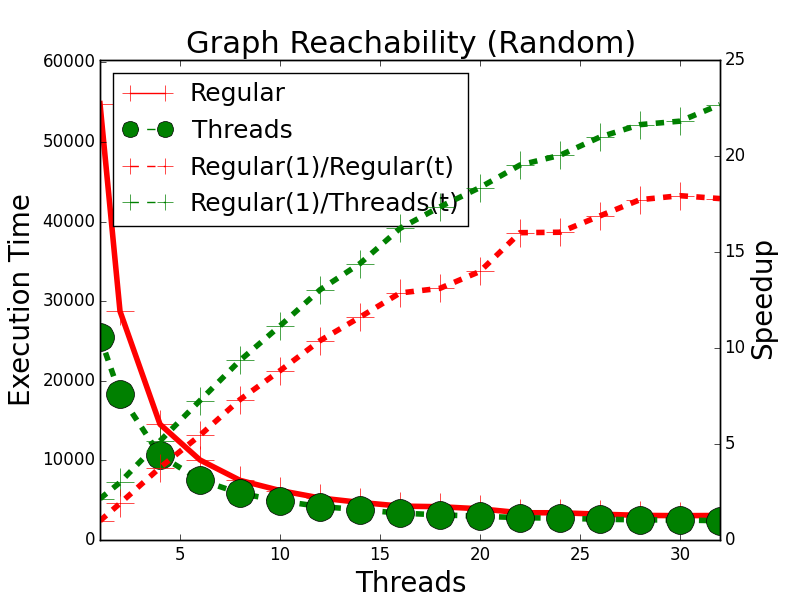
\includegraphics[width=\textwidth]{experiments/threads/cmp-search-random.png}
           \caption{Random is a graph with 50000 nodes and 1052674
              edges. The dataset makes 20 graph queries
              to 5\% of the graph's nodes.}
           \label{fig:threads:search_random}
        \end{subfigure}
        \spacing
        \begin{subfigure}[b]{\plotsize\textwidth}
           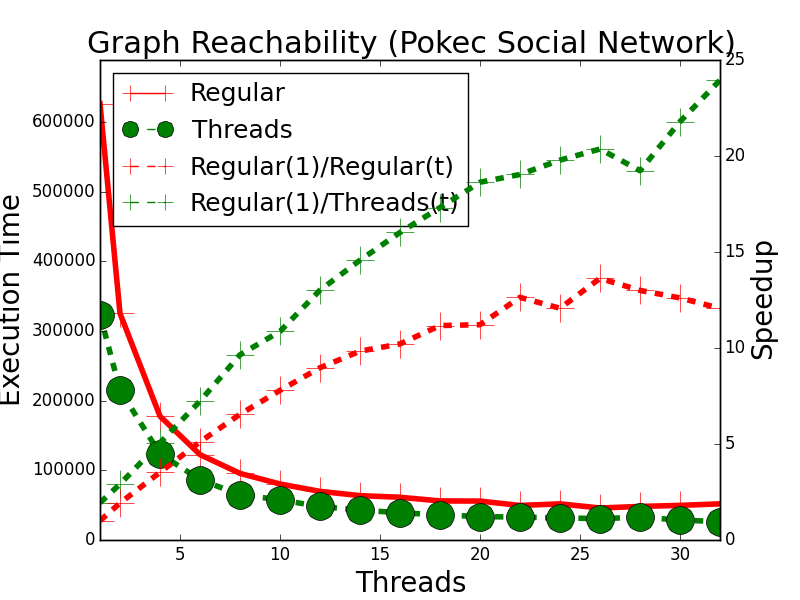
\includegraphics[width=\textwidth]{experiments/threads/cmp-search-pokec.png}
           \caption{Pokec has 1632803 nodes and 30622564 edges. The dataset
           makes 3 graph queries to 1\% of the graph's nodes.}
           \label{fig:threads:search_pokec}
        \end{subfigure} \\
        \caption{Measuring the performance of the graph reachability program
        when using thread facts.}
        \label{fig:threads:results_search}
\end{figure}

The graph reachability program shows how to introduce complex coordination
policies between threads by reasoning about the state of each thread. In
addition, the use of linear logic programming makes it easier to prove
properties of the program since computation is done by applying controlled
changes to the state.


\clearpage


\section{Implementation Changes}
The compilation and runtime system described in
Chapter~\ref{chapter:implementation} requires ysome changes in both the compiler
and in the runtime system to support thread-based facts.

\subsection{Compiler}

The compiler needs to recognize rules that use thread facts. For thread rules,
the compiler checks if the rule's body is using facts from the same thread by
checking the first argument of each fact. For mixed rules, the rule's body may
use a thread \code{T} and a node \code{A} and all the node facts have to use
\code{A}, while all threads facts must use \code{T} as the first argument. If
the programmer was to retrieve either the thread or the node for the current
computation, she may use \code{running(T, A)}.

Once rules are type checked, the iteration code for thread-based facts
needs to change. The database iterator will refer to the current thread in order to
fetch candidate facts since using the standard node database will return an
empty iterator. The runtime API used for inserting thread facts is also
different since they have to be added to the thread's database.

\subsection{Runtime}

Each thread has its own database of facts that is identical to a regular node
but only contains thread predicates. The major difference between a regular node
and a thread node is that a thread node is never put into the work queue of its
thread. As shown in the updated work loop presented in
Fig.~\ref{alg:threads:work_loop}, the thread node executes alongside the regular
node when $TH.process\_node$ is called. It is also important to note that,
before a thread becomes idle, it may have potential candidate thread rules that
are now derivable because another thread has derived thread facts in the current
thread. Note that it is entirely possible to have programs that only deal with
thread facts. These kinds of programs use only explicit parallelism.

\begin{figure}
\begin{algorithm}[H]
\KwData{Thread TH, THREADS}
\While{true}{
  $node \longleftarrow TH.work\_queue.pop\_node()$ \;
  \uIf{$node$}{
        \tcc{Have to use the thread's node}
        \underline{$TH.process\_node(node, TH.my\_node)$}\;
  }
  \Else{
     $target \longleftarrow random(len(THREADS))$\;
     $i \longleftarrow 0$\;
     \For{$i < len(THREADS)$}{
        $target \longleftarrow (target + 1) \% len(THREADS)$\;
        $nodes = THREADS[target].steal\_half()$\;
        \If{$len(nodes) > 0$}{                                                                                                    $TH.work\_queue.add\_to\_queue(nodes)$\;
           break\;
        }
        $i \longleftarrow i + 1$\;
     }
     \If{$len(TH.work\_queue) == 0$}{
        \tcc{The thread's node may have candidate rules using incoming thread facts}
        \underline{$TH.process\_node(nil, TH.my\_node)$}\;
        $TH.become\_idle()$\;
        \If{$TH.synchronize\_termination()$}{
           \Return{}\;
        }
        $TH.become\_active()$\;
     }
  }
}
\end{algorithm}
\caption{Thread work loop updated to take into account thread-based facts.
New and modified code is underlined.}
\label{alg:threads:work_loop}
\end{figure}

Thread facts also add points of synchronization the runtime system. For
instance, when a rule derives a new thread fact on another thread, it needs to
synchronize with that thread (using locks) to add the facts to the thread's
database.

\subsubsection{Matching Rules}

Matching rules using thread facts requires special care since some rules may
require both facts from a node and from a thread. Before a node is executed, the
matching engine of the regular node is updated to take into account the facts in
the thread. If the mixed rules are activated, they need to be executed, even if
they have failed under a different node. The reason is simple: the rule
constraints may now hold under the current node's database and therefore the
rule needs to be executed again.

\subsection{Graph Of Threads}

We added several helpful predicates that allow the programmer to inspect the
graph of threads and reason about the state of computation as it relates to
threads.

\begin{itemize}
   \item \code{\bang thread-list(T, L)}: Fact instantiated in all threads where
      \code{L} is a list of all threads executing in the system.

   \item \code{\bang other-thread(T1, T2)}: Connects thread \code{T1} to all the
      other threads \code{T2} executing in the system.

   \item \code{\bang leader-thread(T, TLeader)}: Fact instantiated in all
      threads where \code{TLeader} refers to a selected thread (usually the
      first thread in \code{L} of \code{\bang thread-list(T, L)}).

   \item \code{running(T, A)}: Used to retrieve the current node \code{A}
      running on thread \code{T}.
\end{itemize}

With the exception of \code{running}, every other fact is added at the beginning
of the program as a persistent axiom.


\section{Applications}

This section presents more applications that demonstrate the usefulness and
power of thread-based facts.

\subsection{Binary Search Trees: Caching Results}
In Section~\ref{sec:language:key_value} we have presented an algorithm for
replacing a key's value in a BST dictionary. To make the program more
interesting, we consider a sequence of $n$ lookup or replace operations for
different keys in the BST (which may or may not be repeated). A single lookup or
replace has worst-case time complexity $\mathcal{O}(h)$ where $h$ is the height
of the BST, therefore performing $n$ operations takes $\mathcal{O}(h \times n)$
time.

In order to reduce the execution time of the new program, we can cache the
search and replace operations so that repeated operations become faster. Instead
of traversing the entire height of the BST, we look in the cache and send the
operation immediately to the node where the key is located. Without thread
facts, we might have cached the results at the root node, however, this is not a
scalable approach as it would introduce a serious bottleneck.

Figure~\ref{code:threads:btree_lookup_cache} shows the updated BST code with a thread
cache. We just added two more predicates, \code{cache} and
\code{cache-size}, that are facts placed in the thread and represent cached
keys and the total size of the cache, respectively. We also added three new
rules that handle the following cases:

\begin{enumerate}
      \item A key is found and is also in the cache
         (lines~\ref{line:threads:kv_rule1_start}-\ref{line:threads:kv_rule2_end})

      \item A key is found but is not in the cache
         (lines~\ref{line:threads:kv_rule2_start}-\ref{line:threads:kv_rule2_end});

      \item A key is in the cache, therefore a \code{replace} fact is
         derived in the target node
         (lines~\ref{line:threads:kv_rule3_start}-\ref{line:threads:kv_rule3_end}).

\end{enumerate}

Note that it is quite easy to extend the cache mechanism to use an LRU type
approach in order to limit the size of the cache.

\begin{figure}[ht]
\begin{Verbatim}[numbers=left,fontsize=\codesize,commandchars=*\{\}]
type left(node, node).
type right(node, node).
type linear value(node, int Key, string Value).
type linear replace(node, int Key, string Value).
type linear cache(thread, node, int).
type linear cache-size(thread, int).

// (1) Key exists and is also in the cache.*label{line:threads:kv_rule1_start}
replace(A, Key, RValue),
value(A, Key, Value),
*textbf{cache(T, A, Key)}
   -o value(A, Key, RValue).
      *textbf{cache(T, A, Key)}.*label{line:threads:kv_rule1_end}

// (2) Key exists and is not in the cache.*label{line:threads:kv_rule2_start}
replace(A, Key, RValue),
value(A, Key, Value),
*textbf{cache-size(T, Total)}
   -o value(A, Key, RValue),
      *textbf{cache-size(T, Total + 1)},
      *textbf{cache(T, A, Key)}.*label{line:threads:kv_rule2_end}

// (3) Cached by the thread.*label{line:threads:kv_rule3_start}
replace(A, RKey, RValue),
*textbf{cache(T, TargetNode, RKey)}
   -o replace(TargetNode, RKey, RValue),
      *textbf{cache(T, TargetNode, RKey)}.*label{line:threads:kv_rule3_end}

replace(A, RKey, RValue),
value(A, Key, Value),
!left(A, B),
RKey < Key
   -o value(A, Key, Value),
      replace(B, RKey, RValue). // go left

replace(A, RKey, RValue),
value(A, Key, Value),
!right(A, B),
RKey > Key
   -o value(A, Key, Value),
      replace(B, RKey, RValue). // go right
\end{Verbatim}
\caption{LM program for performing lookups in a BST with a thread cache.}
\label{code:threads:btree_lookup_cache}
\end{figure}


\subsection{PowerGrid Problem}
Consider a power grid with $C$ consumers and $G$ generators. We are interested
in connecting each consumer to a single generator, but each generator has a
limited capacity and the consumer draws a certain amount of power from the
generator. A valid power grid is built in such a way that all consumers are
serviced by a generator and that no generator is being overdrawn by too many
consumers. Although consumers and generators may be connected through a complex
network, we analyze the simple case where any consumer is able to attach to any
generator.

\begin{wrapfigure}{r}{0.5\textwidth}
   \begin{center}
      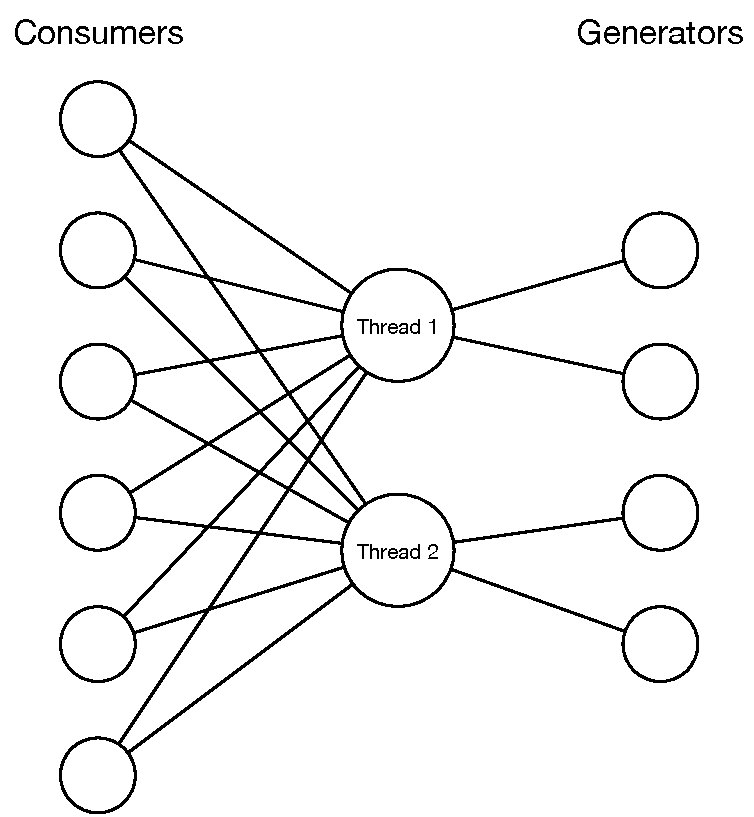
\includegraphics[width=1\linewidth]{figures/threads/powergrid.pdf}
   \end{center}
   \mycap{Configuration of a powergrid with 6 consumers, 4
      generators and 2 threads, with each thread responsible for 2 generators.}
   \label{fig:threads:powergrid}
\end{wrapfigure}

A straightforward distributed implementation for the PowerGrid problem requires
that each consumer is able to connect to any generator. Once a generator
receives a connection request, it may or may not accept it. If the generator has
no power available for the new consumer, it will disconnect from it and the
consumer must select another generator. This randomized algorithm works but may
take a long time to converge, depending on the amount of power available in the
generators. Figure~\ref{code:threads:powergrid} shows the LM code for this
solution. Consumer and generators node types are declared in
lines~\ref{line:threads:pg_decl1}-\ref{line:threads:pg_decl2} using the
\code{node} declaration, allowing us to have different predicates for consumers
and generators. The \code{consumer} and \code{generator} types become a subtype
of \emph{node}, that is, $consumer <: node$ and $generator <: node$.  These
subtypes allow us to declare initial facts that only apply to either the
\code{consumer} or \code{generator} subtype.

\begin{figure}[h!]
\begin{LineCode}[commandchars=*\#\&]
node generator.*label#line:threads:pg_decl1&*hfill// Type declaration
node consumer.*label#line:threads:pg_decl2&
type linear capacity(generator, int Total, int Used).*hfill// Predicate declaration
type linear connected-to(generator, consumer, int).
type linear connected-to-list(generator, list consumer).
type power(consumer, int).
type linear disconnected(consumer).
type linear connected(consumer, generator).
type generators(consumer, list generator).
type linear fails(generator, int).
type linear random-reconnect(generator).
type linear reconnect(consumer).
type linear connect(generator, consumer, int).
type linear disconnect(consumer, generator).

fails(G, Fails), Fails > maxfails*label#line:threads:pg_recon1&*hfill// Rule 1: disconnect one consumer
   -o random-reconnect(G).

capacity(G, Total, Used), random-reconnect(G),*hfill// Rule 2: disconnect one consumer
connected-to-list(G, L), L <> [], C = nth(L, randint(length(L))),
connected-to(G, C, Power)
   -o fails(G, 0), capacity(G, Total, Used - Power),
      connected-to-list(G, remove(L, C)), disconnect(C, G).

capacity(G, Total, Used), random-reconnect(G)*hfill// Rule 3: unable to disconnect one consumer
   -o capacity(G, Total, Used), fails(G, 0).*label#line:threads:pg_recon2&

connect(G, C, Power), capacity(G, Total, Used),*label#line:threads:pg_gen1&*hfill// Rule 4: connect consumer
fails(G, Fails), connected-to-list(G, L), Used + Power <= Total
   -o capacity(G, Total, Used + Power),
      fails(G, max(Fails - 1, 0)), connected-to(G, C, Power),
      connected-to-list(G, [C | L]).*label#line:threads:pg_gen2&

connect(G, C, Power), capacity(G, Total, Used),*label#line:threads:pg_fail1&*hfill// Rule 5: unable to connect consumer
Used + Power > Total, fails(G, Fails)
   -o capacity(G, Total, Used), disconnect(C, G),
      fails(G, Fails + 1).*label#line:threads:pg_fail2&

!generators(C, L), !power(C, Power),*label#line:threads:pg_connect1&*hfill// Rule 6: connect to a generator
reconnect(C), disconnected(C),
G = nth(L, randint(num-generators))
   -o connected(C, G), connect(G, C, Power).*label#line:threads:pg_connect2&

disconnect(C, G), connected(C, G)*hfill// Rule 7: finish disconnection
   -o disconnected(C), reconnect(C).

connected-to-list(G, []). fails(G, 0).*hfill// Initial facts
disconnected(C). reconnect(C). !generators(C, all-generators).
\end{LineCode}
\mycap{LM code for the regular PowerGrid program.}
\label{code:threads:powergrid}
\end{figure}

An example PowerGrid configuration with its initial facts is presented in
Fig.~\ref{code:threads:powergrid_init}. Consumers have a persistent fact
\code{!power(A, P)}, where \code{P} is the amount of power required by the
consumer. Consumers also start with a
\code{reconnect} fact that is used in
lines~\ref{line:threads:pg_connect1}-\ref{line:threads:pg_connect2} in order to
randomly select a generator from list \code{L} in the \code{!generators(A, L)}
fact. The generators have a \code{connect-to-list(A, L)} fact that manages the
list of connected consumers. The generator fact \code{capacity(A, Total, Used)},
stores the \code{Total} capacity of the generator and the amount of power
currently being \code{Used} (\code{Used < Total} at any point in the program).

Consumers and generators complete a connection when the generator receives a
\code{connect} fact which is used in
lines~\ref{line:threads:pg_gen1}-\ref{line:threads:pg_gen2} when the generator
has enough power for the new consumer. When there is not enough power
(\code{Used + Power > Total}), the generator disconnects the consumer in
lines~\ref{line:threads:pg_fail1}-\ref{line:threads:pg_fail2}. Note that each
generator maintains a \code{fail} fact that counts the number of times the
consumers have failed to connected. If there is too many failures, then the
generator decides to disconnect one consumer already connected in
lines~\ref{line:threads:pg_recon1}-\ref{line:threads:pg_recon2}, allowing for
different combinations to happen. In Fig.~\ref{code:threads:powergrid_final} we
present the final database of the example PowerGrid configuration, which shows
that all consumers have been able to find a suitable generator.

\begin{figure}[h!]
\begin{LineCode}[commandchars=*\#\&]
const generators = [@7, @8, @9, @10].

reconnect(@1).   !generators(@1, generators).   !power(@1, 5).
reconnect(@2).   !generators(@2, generators).   !power(@2, 10).
reconnect(@3).   !generators(@3, generators).   !power(@3, 5).
reconnect(@4).   !generators(@4, generators).   !power(@4, 10).
reconnect(@5).   !generators(@5, generators).   !power(@5, 10).
reconnect(@6).   !generators(@6, generators).   !power(@6, 5).

connected-to-list(@7, []).    capacity(@7, 15, 0).   fail(@7, 0).
connected-to-list(@8, []).    capacity(@8, 15, 0).   fail(@8, 0).
connected-to-list(@9, []).    capacity(@9, 10, 0).   fail(@9, 0).
connected-to-list(@10, []).   capacity(@10, 5, 0).   fail(@10, 0).
\end{LineCode}
\mycap{Initial facts for a PowerGrid configuration of 6 consumers and 4 generators.}
\label{code:threads:powergrid_init}
\end{figure}

\begin{figure}[h!]
\begin{LineCode}[commandchars=*\#\&]
connected(@1, @7).    !power(@1, 5).
connected(@2, @7).    !power(@2, 10).
connected(@3, @8).    !power(@3, 5).
connected(@4, @8).    !power(@4, 10).
connected(@5, @9).    !power(@5, 10).
connected(@6, @10).   !power(@6, 5).

connected-to-list(@7, [@1, @2]).   connected-to(@7, @1, 5).   connected-to(@7, @2, 10).
connected-to-list(@8, [@3, @4]).   connected-to(@8, @3, 5).   connected-to(@8, @4, 10).
connected-to-list(@9, [@5]).       connected-to(@9, @5, 10).
connected-to-list(@10, [@6]).      connected-to(@10, @6, 5).
capacity(@7, 15, 15).
capacity(@8, 15, 15).
capacity(@9, 10, 10).
capacity(@10, 5, 5).
\end{LineCode}
\mycap{Final facts for a PowerGrid configuration of 6 consumers and 4 generators.}
\label{code:threads:powergrid_final}
\end{figure}

The issue with this initial implementation presented in
Fig.~\ref{code:threads:powergrid} is that it lacks a global view of the problem,
which introduces inefficiencies and more communication between consumers and
generators. A better algorithm will require a more sophisticated communication
pattern between the nodes. As we have seen before, thread local facts are an
excellent mechanism to introduce a global view of the problem without
complicating the original algorithm written in a declarative style. For our
solution, we will partition the set of generators $G$ among the threads in the
system and make each thread assume the ownership of its generators. Each thread
can then process consumers with a global view over its set of generators,
allowing the immediate assignment of consumers to generators.
Figure~\ref{fig:threads:powergrid} shows how the configuration presented
previously is adjusted to take into account the number of available threads.

The LM code using thread facts shown in Fig.~\ref{code:threads:powergridt}. It uses
4 thread predicates: \code{thread-connected-to} and
\code{thread-connected-to-list} assign consumers to the generators owned by the
thread; \code{thread-capacity} stores the capacity of each generator assigned to
the thread; and \code{thread-total-capacity} provides a capacity overview of all
the generators owned by the thread.  The program starts with the rule in
lines~\ref{line:threads:pgt_start1}-\ref{line:threads:pgt_start2} by moving
generators to their corresponding threads using \code{set-thread}. Once the
generator is executing on the proper thread, the rule in
lines~\ref{line:threads:pgt_moved1}-\ref{line:threads:pgt_moved2} is derived
with the \code{just-moved} coordination fact and the state of the thread is
initialized. Consumers connect with the thread's generators with the rule in
lines~\ref{line:threads:pgt_con1}-\ref{line:threads:pgt_con2} by selecting the
first generator with enough power and then by updating the state of the thread.
Otherwise, if the thread does not have a suitable generator, a generator is
randomly selected using the method described before. For such cases, the thread
assigned with the selected generator will derive the rules in
lines~\ref{line:threads:pgt_gen1}-\ref{line:threads:pgt_gen2} and the thread
state is updated accordingly.

\begin{figure}[h!]
\begin{LineCode}[fontsize=\scriptsize,commandchars=*\#\&]
type linear thread-connected-to(thread, generator, consumer, int).*hfill// Predicate declaration
type linear thread-connected-to-list(thread, generator, list consumer).
type linear thread-capacity(thread, generator, int, int).
type linear thread-total-capacity(thread, int, int).
type linear start(generator).

start(G), !generator-id(G, Id)*label#line:threads:pgt_start1&
   -o set-thread(G, Id % @threads).*label#line:threads:pgt_start2&

just-moved(G), capacity(G, Total, Used), thread-total-capacity(T, TotalCapacity, TotalUsed)*label#line:threads:pgt_moved1&
   -o thread-connected-to-list(T, G, []), thread-capacity(T, G, Total, Used),
      thread-total-capacity(T, Total + TotalCapacity, Used + TotalUsed).*label#line:threads:pgt_moved2&

fails(G, Fails), Fails > maxfails
   -o random-reconnect(G).

thread-capacity(T, G, Total, Used), thread-total-capacity(T, TotalCapacity, TotalUsed),
random-reconnect(G), thread-connected-to-list(T, G, L), L <> [], C = nth(L, randint(length(L))),
thread-connected-to(T, G, C, Power), NewUsed = Used - Power
   -o fails(G, 0), thread-capacity(T, G, Total, NewUsed),
      thread-total-capacity(T, TotalCapacity, TotalUsed - Power),
      thread-connected-to-list(T, G, remove(L, C)), disconnect(C, G).

random-reconnect(G) -o fails(G, 0).

connect(G, C, Power), thread-total-capacity(T, TotalCapacity, TotalUsed),*label#line:threads:pgt_gen1&
thread-capacity(T, G, Total, Used), fails(G, Fails), thread-connected-to-list(T, G, L),
NewUsed = Used + Power, NewUsed <= Total
   -o thread-capacity(T, G, Total, NewUsed),
      thread-total-capacity(T, TotalCapacity, TotalUsed + Power),
      fails(G, max(Fails - 1, 0)), thread-connected-to(T, G, C, Power),
      thread-connected-to-list(T, G, [C | L]).*label#line:threads:pgt_gen11&

connect(G, C, Power), thread-capacity(T, G, Total, Used), Used + Power > Total, fails(G, Fails)
   -o thread-capacity(T, G, Total, Used), disconnect(C, G), fails(G, Fails + 1).*label#line:threads:pgt_gen2&

!power(C, Power), reconnect(C), disconnected(C), thread-total-capacity(T, TotalCapacity, TotalUsed),*label#line:threads:pgt_con1&
TotalNewUsed = TotalUsed + Power, NewUsed <= TotalCapacity,
thread-capacity(T, G, Total, Used), thread-connected-to-list(T, G, ConnectList),
NewUsed = Used + Power, NewUsed <= Total
   -o connected(C, G), thread-capacity(T, G, Total, NewUsed),
      thread-connected-to-list(T, G, [C | ConnectList]), thread-connected-to(T, G, C, Power),
      thread-total-capacity(T, TotalCapacity, TotalNewUsed).*label#line:threads:pgt_con2&

!generators(C, L), !power(C, Power), reconnect(C), disconnected(C), G = nth(L, randint(num-generators))*label#line:threads:pgt_conn1&
   -o connected(C, G), connect(G, C, Power).*label#line:threads:pgt_conn2&

disconnect(C, G), connected(C, G)
   -o disconnected(C), reconnect(C).

thread-total-capacity(T, 0, 0).*hfill// Initial facts
fails(G, 0).  disconnected(C).  reconnect(C).  !generators(C, all-generators).  start(G).
\end{LineCode}
\mycap{LM code for the optimized PowerGrid program.}
\label{code:threads:powergridt}
\end{figure}

The experimental results for the PowerGrid program are presented in
Fig.~\ref{fig:threads:results_powergrid}. In the plots, we show the run time of
the version without thread facts, named \textbf{Regular}, and the version using
thread facts, called \textbf{Threads}. We also show the speedup of the
\textbf{Threads} and \textbf{Regular} versions against the \textbf{Regular}
version with 1 thread.  We experimented with four datasets:

\begin{enumerate}
      \item 0.5 M C / 2000 G: Half a million consumers connected to 2000
         generators. This is the baseline dataset.

      \item 0.5 M C / 64 G: Half a million consumers connected to 64
         generators. This is similar to the previous dataset, but the number of
         generators is much smaller.

      \item 1 M C / 4000 G / Low Variability: 1 million consumers connected to
         4000 generators. The capacity of each generator has low variability so
         that each generator has a similar capacity.

      \item 1 M C / 4000 G / High Variability: 1 million consumers connected to
         4000 generators. The capacity of each generator has high variability so
         that some generators have no capacity or three times the average the
         capacity.

\end{enumerate}

All the datasets were generated randomly so that the total capacity of the
generators is about 2\% more than the required consumer capacity. The capacity
of each generator is generated randomly and, except for the last two datasets,
the capacity is between 0 and twice the average capacity (total capacity divided
by the number of generators).

The first important observation relates to the first two datasets. In the 0.5 M
C / 2000 G, the \textbf{Threads} version has more than a 150-fold speedup for 32
threads while the 0.5 M C / 64 G dataset only reaches a 70-fold speedup. Having
only 64 generators instead of 2000 makes it harder to scale the program since
there is only a few generators to distribute among threads. However, it must be
noted that the 0.5 M C / 64 G dataset performs proportionally faster when using
1 thread than the 2000 G dataset since that one thread has a small number of
generators to choose from when processing consumers. The rule that assigns
generators to consumers
(lines~\ref{line:threads:pgt_gen1}-\ref{line:threads:pgt_gen11} in
Fig.~\ref{code:threads:powergridt}) needs to
iterate through all the generators to find one with enough power to handle the
consumer, therefore, a smaller number of generators is a clear advantage over
having many generators in the case of using just 1 thread.

\begin{figure}[]
        \centering
        \begin{subfigure}[b]{\plotsize\textwidth}
           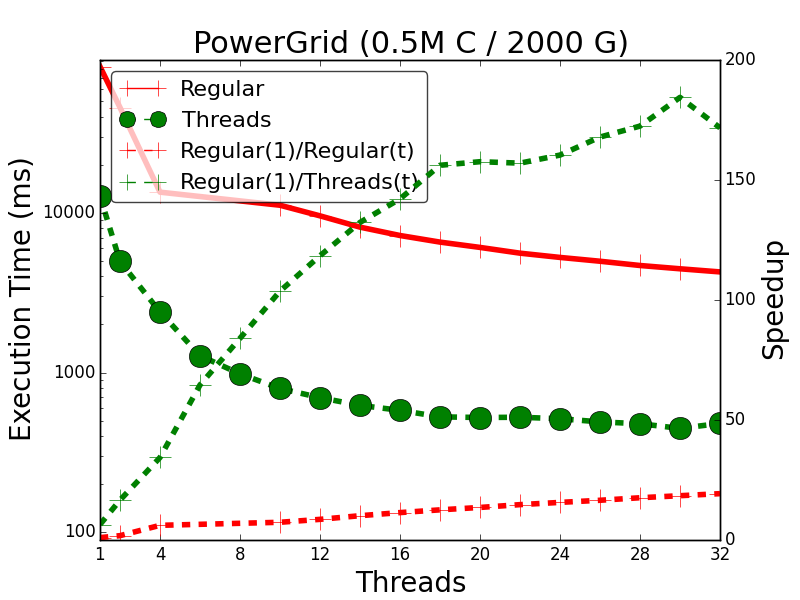
\includegraphics[width=\textwidth]{experiments/threads/cmp-powergrid-500000C2000G.png}
           \mycap{}
           \label{fig:threads:powergrid1}
        \end{subfigure}
        ~
        \begin{subfigure}[b]{\plotsize\textwidth}
           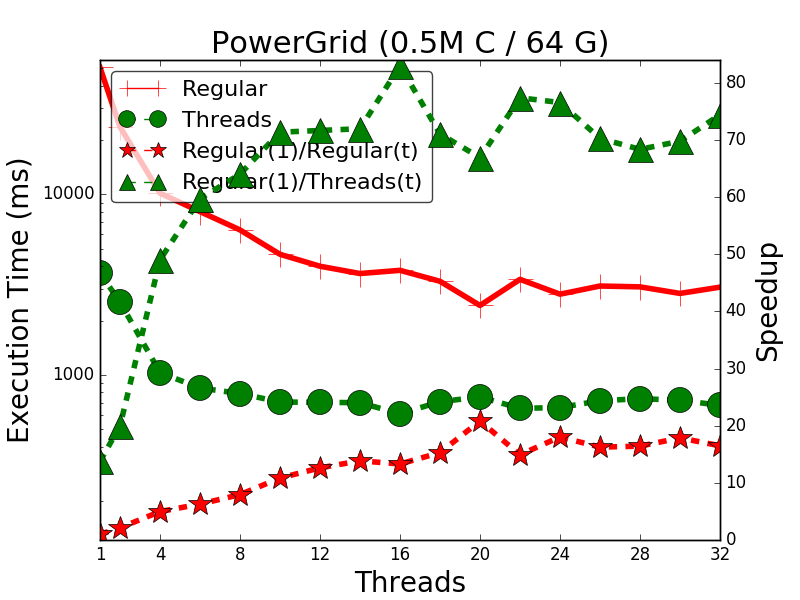
\includegraphics[width=\textwidth]{experiments/threads/cmp-powergrid-500000C64G.png}
           \mycap{}
           \label{fig:threads:powergrid2}
        \end{subfigure} \\
        \begin{subfigure}[b]{\plotsize\textwidth}
           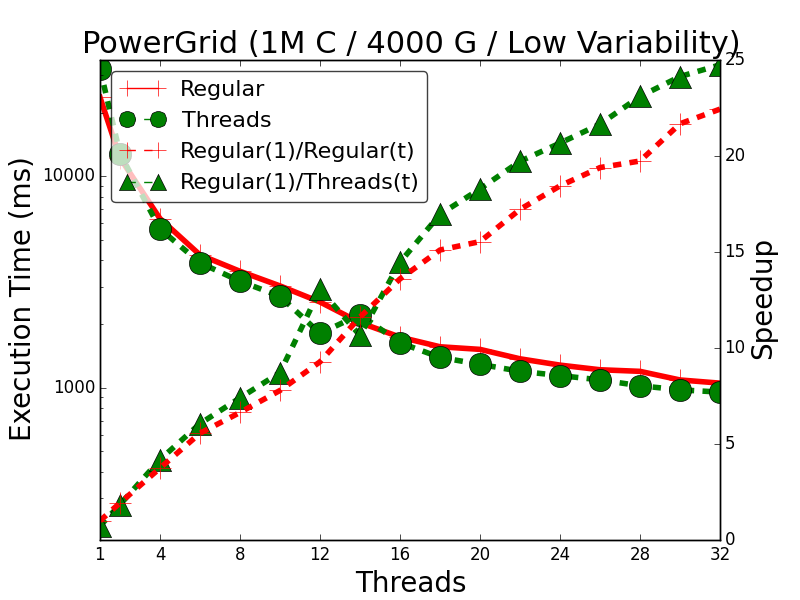
\includegraphics[width=\textwidth]{experiments/threads/cmp-powergrid-1M4000C-low.png}
           \mycap{}
           \label{fig:threads:powergrid3}
        \end{subfigure} ~
        \begin{subfigure}[b]{\plotsize\textwidth}
           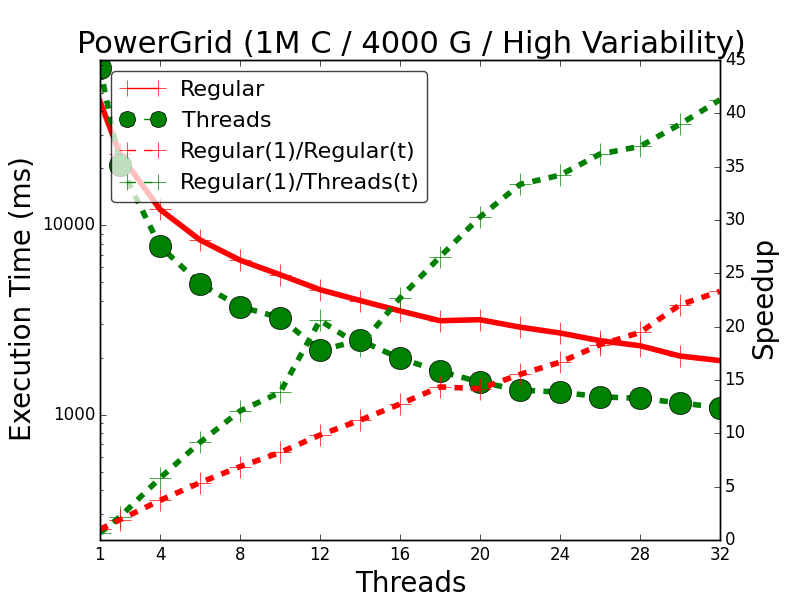
\includegraphics[width=\textwidth]{experiments/threads/cmp-powergrid-1M4000C-high.png}
           \mycap{}
           \label{fig:threads:powergrid4}
        \end{subfigure} \\
        \mycap{Measuring the performance of the PowerGrid program
        when using thread facts.}
        \label{fig:threads:results_powergrid}
\end{figure}

The second important observation relates to the last two datasets where we
experimented with a variable capacity for the generators. For the Low
Variability dataset, the consumers have identical capacities, while in the High
Variability dataset, generators have a more variable capacity, which should make
it harder for the algorithm to find a valid generator/consumer assignment.  Our
results show exactly that: the Low Variability shows a small difference between
the \textbf{Regular} and \textbf{Threads} version, while in the High Variability
dataset, the \textbf{Threads} version is much faster than the \textbf{Regular}
version. However, for the High Variability dataset, we were expecting a speedup
that was closer to the 0.5 M C / 2000 G dataset, since the number of generators
is much higher. Furthermore, if we compare the run times of the \textbf{Regular}
and \textbf{Threads} version when using 1 thread, we notice that the
\textbf{Threads} version is actually slower. As noted before, this may be due to
the fact that the LM rule for assigning generators to consumers needs to perform
a linear scan on the available generators to find a suitable generator which
then negatively impacts performance. This is a clear drawback of the logic
programming model that could potentially be solved by maintaining a sorted list
of \texttt{thread-capacity} facts.

In Table~\ref{table:threads:powergrid_stats}, we present several fact statistics
that compare the \textbf{Regular} version with the \textbf{Threads} version when
executing with multiple threads. The \textbf{\# Derived} column indicates the
number of derived facts, \textbf{\# Deleted} indicates the number of retracted
facts, while \textbf{\# Final} is the number of facts in the database after the
program terminates. The table results clearly show that using thread-based facts
results in a decrease in the number of generated facts, which is more
significant in the 0.5M C / 2000 G dataset (10-fold reduction). The table also
explains why this dataset performs much better than the 1M C / 4000 G High
Variability dataset, which only sees a 2-fold reduction in derived facts.

When comparing the number of facts derived when using a different number of
threads, the overall trend indicates that having more threads slightly increases
the number of derived facts. This is especially true for the 0.5 M C / 64 G
datasets, where twice as many facts are generated when using 32 threads when
compared to 1 thread.

\begin{table}[ht]
   \begin{center}
      \begin{tabular}{c | c || c c | c c | c c} \hline
	 \multirow{2}{*}{\textbf{Dataset}} & \multirow{2}{*}{\textbf{Threads}} & \multicolumn{2}{c|}{\textbf{\# Derived}} & \multicolumn{2}{c|}{\textbf{\# Deleted}} & \multicolumn{2}{c}{\textbf{\# Final}}\\
	 & & Regular & Threads & Regular & Threads & Regular & Threads\\ \hline \hline
\multirow{7}{*}{0.5M C / 2000 G}  & 1 &  49.7M & 4.2M &  48.2M & 2.5M &  2.5M & 2.5M \\
 & 2 &  48.5M & 4.4M &  47.7M & 2.5M &  2.5M & 2.5M \\
 & 4 &  49.4M & 4.1M &  47.9M & 2.6M &  2.5M & 2.5M \\
 & 8 &  49.4M & 4.10M &  47.9M & 2.5M &  2.5M & 2.5M \\
 & 16 &  50.8M & 4.1M &  49.3M & 2.6M &  2.5M & 2.5M \\
 & 24 &  49.8M & 4.2M &  48.3M & 2.7M &  2.5M & 2.5M \\
 & 32 &  49.3M & 4.6M &  47.8M & 3.1M &  2.5M & 2.5M \\
	\hline
\multirow{7}{*}{0.5M C / 64 G}  & 1 &  20.2M & 4.3M &  18.5M & 2.5M &  2.5M & 2.5M \\
 & 2 &  19.9M & 4.2M &  18.4M & 2.7M &  2.5M & 2.5M \\
 & 4 &  20.7M & 4.4M &  18.5M & 2.9M &  2.5M & 2.5M \\
 & 8 &  19.9M & 5.6M &  18.4M & 4.10M &  2.5M & 2.5M \\
 & 16 &  19.8M & 6.8M &  18.3M & 5.3M &  2.5M & 2.5M \\
 & 24 &  19.7M & 8.4M &  18.2M & 6.9M &  2.5M & 2.5M \\
 & 32 &  19.9M & 9.3M &  18.4M & 7.5M &  2.5M & 2.5M \\
	\hline
\multirow{7}{*}{\makecell{1M C / 4000 G \\Low Variability}}  & 1 &  9.4M & 7.5M &  6.4M & 4.5M &  5.1M & 5.1M \\
 & 2 &  9.4M & 7.5M &  6.4M & 4.5M &  5.1M & 5.1M \\
 & 4 &  9.4M & 7.5M &  6.4M & 4.5M &  5.1M & 5.1M \\
 & 8 &  9.4M & 7.6M &  6.4M & 4.6M &  5.1M & 5.1M \\
 & 16 &  9.4M & 7.5M &  6.4M & 4.5M &  5.1M & 5.1M \\
 & 24 &  9.4M & 7.6M &  6.3M & 4.6M &  5.1M & 5.1M \\
 & 32 &  9.3M & 7.5M &  6.3M & 4.5M &  5.1M & 5.1M \\
	\hline
\multirow{7}{*}{\makecell{1M C / 4000 G \\High Variability}}  & 1 &  16.4M & 8.8M &  13.4M & 5.8M &  5.1M & 5.1M \\
 & 2 &  16.5M & 8.8M &  13.5M & 5.8M &  5.1M & 5.1M \\
 & 4 &  16.5M & 8.8M &  13.4M & 5.8M &  5.1M & 5.1M \\
 & 8 &  16.5M & 8.9M &  13.5M & 5.9M &  5.1M & 5.1M \\
 & 16 &  16.5M & 8.8M &  13.5M & 5.8M &  5.1M & 5.1M \\
 & 24 &  16.5M & 9.3M &  13.5M & 6.2M &  5.1M & 5.1M \\
 & 32 &  16.5M & 9.6M &  13.5M & 6.5M &  5.1M & 5.1M \\
	\hline
\end{tabular}

   \end{center}

   \mycap{Measuring the reduction in derived facts when using thread-based
   facts.}
   \label{table:threads:powergrid_stats}
\end{table}

%\clearpage


\subsection{Splash Belief Propagation}\label{sec:coordination:bp}
Approximation algorithms can obtain significant benefits from using customized
scheduling policies since they follow important statistical properties and thus
can trade correctness for faster convergence. An example of such algorithm is
the Loopy Belief Propagation (LBP)~\cite{Murphy99loopybelief}. LBP is an
approximate inference algorithm used in graphical models with cycles which
employs a sum-product message passing algorithm where nodes exchange messages
with their immediate neighbors and apply some computations to the messages
received.

\begin{figure}[h]
   \begin{center}
      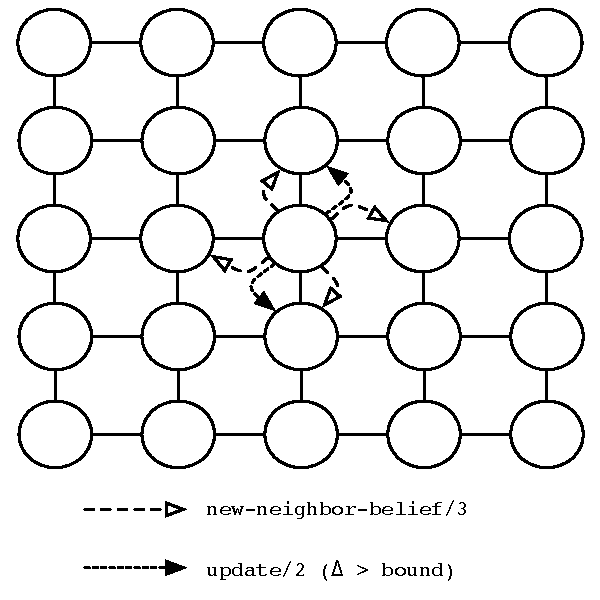
\includegraphics[width=0.3\textwidth]{figures/bp/bp.pdf}
   \end{center}

   \mycap{LBP communication patterns. \code{new-neighbor-belief} facts are
   sent to the neighborhood when the node's belief value is updated. If the new
   value sent to the neighbor differs significantly from the value sent before
   the current the round, then an \code{update} fact is also sent (to the node
   above and below in this case).}

\label{fig:coordination:bp}
\end{figure}

LBP is an algorithm that maps very well to the graph-based model of LM. The
original algorithm computes the belief of all nodes using several iterations
with synchronization between iterations. However, it is possible to avoid the
synchronization step, if we take advantage of the fact that LBP will converge
even when using an asynchronous approach. So, instead of computing the belief
iteratively, we keep track of all messages sent/received (and overwrite them
when we receive a new one) and recompute the belief asynchronously.
Figure~\ref{fig:coordination:bp} presents the communication patterns of the
program, while Fig.~\ref{code:coordination:bp} presents the LM code for the
asynchronous version of LBP.

\begin{figure}[ht]
\begin{Verbatim}[numbers=left, fontsize=\codesize, commandchars=\*\#\&]
type list float belief.*hfill// Type declaration.

type potential(node, belief).*hfill// Predicate declaration
type edge(node, node).
type linear neighbor-belief(node, node, belief).
type linear new-neighbor-belief(node, node, belief).
type linear sent-neighbor-belief(node, node, belief).
type linear check-residual(node, float, node).
type linear belief(node, belief).
type linear update-messages(node, belief).
type linear update(node).

neighbor-belief(A, B, Belief),*label#line:coord:bp_first1&*hfill// Rule 1: update neighbor belief value
new-neighbor-belief(A, B, NewBelief)
   -o neighbor-belief(A, B, NewBelief).*label#line:coord:bp_first2&

check-residual(A, Residual, B),*label#line:coord:bp_check1&*hfill// Rule 2: check residual
Residual > bound
   -o update(B).

check-residual(A, _, _) -o 1.*label#line:coord:bp_check2&*hfill// Rule 3: check residual

update-messages(A, NewBelief),*hfill// Rule 4: compute belief to be sent to a neighbor node*label#line:coord:bp_iterate1&
   -o {B, OldIn, OldOut, Cavity, Convolved, OutMessage, Residual |
         !edge(A, B),
         neighbor-belief(A, B, OldIn),
         sent-neighbor-belief(A, B, OldOut),
         Cavity = normalize(divide(NewBelief, OldIn)),
         Convolved = normalize(convolve(global-potential, Cavity)),
         OutMessage = damp(Convolved, OldOut, damping)
         Residual = residual(OutMessage, OldOut)
         -o check-residual(A, Residual, B),
            new-neighbor-belief(B, A, OutMessage),
            neighbor-belief(A, B, OldIn),
            sent-neighbor-belief(A, B, OutMessage)}.*label#line:coord:bp_iterate2&

*label#line:coord:bp_last1&
update(A), update(A) -o update(A).*label#line:coord:bp_update&*hfill// Rule 5: prune redundant update operations

update(A),*hfill// Rule 6: initiate update operation*label#line:coord:bp_update1&
!potential(A, Potential),
belief(A, MyBelief)
   -o [sum Potential => Belief; B, Belief |*label#line:coord:bp_agg1&
         neighbor-belief(A, B, Belief) -o
         neighbor-belief(A, B, Belief) ->
         Normalized = normalizestruct(Belief),
         update-messages(A, Normalized), belief(A, Normalized)].*label#line:coord:bp_last2&*label#line:coord:bp_update2&*label#line:coord:bp_agg2&
\end{Verbatim}

\mycap{LM code for the asynchronous version of the Loopy Belief Propagation
problem.}

\label{code:coordination:bp}
\end{figure}

\clearpage

Belief values are arrays of floats and are represented by \code{belief/2} facts.
The first rule (lines~\ref{line:coord:bp_first1}-\ref{line:coord:bp_first2})
updates a given neighbor belief whenever a new belief value is received. This is
the highest priority rule since we want to update the neighbor beliefs before
doing anything else. In order to store the belief values of the neighbor nodes,
we use \code{neighbor-belief/3} facts, where the second argument is the neighbor
address and the third argument is the belief value.

The last two rules (lines~\ref{line:coord:bp_last1}-\ref{line:coord:bp_last2})
update the belief value of a node. An \code{update} fact starts the process.
The first rule (line~\ref{line:coord:bp_update}) simply removes redundant
\code{update} facts and the second rule
(lines~\ref{line:coord:bp_update1}-\ref{line:coord:bp_update2}) performs the
belief update by aggregating all the neighbor belief values. The aggregate in
lines~\ref{line:coord:bp_agg1}-\ref{line:coord:bp_agg2} also derives copies of
the neighbors beliefs that need to be consumed in order to compute the belief
value that is going to be sent to the target neighbor. The aggregate uses a
custom accumulator that takes two arrays and adds the floating point numbers at
each index of the array.

The rule in lines~\ref{line:coord:bp_iterate1}-\ref{line:coord:bp_iterate2}
iterates through the neighbor belief values and sends new belief values by
performing the appropriate computations on the new belief value of the current
node and on the belief value sent previously. For each neighbor update, we also
check in lines~\ref{line:coord:bp_check1}-\ref{line:coord:bp_check2} if the
change in belief values is greater than \code{bound} (a program constant) and
then force the neighbor nodes to update their belief values by deriving
\code{update(B)}. This allows neighbor nodes to use updated neighbor values and
recompute their own belief values using more up-to-date information. The
computation of belief values will then start to converge to their true belief
values, independently of the node scheduling used.

However, if we prioritize nodes that receive new neighbor belief values with a
larger \code{Residual} then we may converge faster.
Figure~\ref{code:coordination:improved_bp} shows the fourth rule modified with a
\code{add-priority} fact, which increases the priority of neighbor nodes when
the source node has large changes in its belief value.

\begin{figure}[h!]
\begin{Verbatim}[numbers=left,commandchars=\\\{\},fontsize=\codesize]
update-messages(A, NewBelief),*hfill// Rule 4: compute belief to be sent to a neighbor node
   -o \{B, OldIn, OldOut, Cavity, Convolved, OutMessage, Residual |
         !edge(A, B),
         neighbor-belief(A, B, OldIn),
         sent-neighbor-belief(A, B, OldOut),
         Cavity = normalize(divide(NewBelief, OldIn)),
         Convolved = normalize(convolve(global-potential, Cavity)),
         OutMessage = damp(Convolved, OldOut, damping)
         Residual = residual(OutMessage, OldOut)
         -o check-residual(A, Residual, B),
            new-neighbor-belief(B, A, OutMessage),
            neighbor-belief(A, B, OldIn),
            \underline{add-priority(B, Residual)},
            sent-neighbor-belief(A, B, OutMessage)\}.
\end{Verbatim}
\mycap{Extending the LBP program with priorities.}
\label{code:coordination:improved_bp}
\end{figure}


The proposed asynchronous approach has shown to be an improvement over the
synchronous version because it leads to faster convergence time. An improved
evaluation strategy is the Splash Belief
Propagation~(SBP)~\cite{Gonzalez+al:aistats09paraml}, where belief values are
computed asynchronously by first building a tree and then updating the beliefs
of each node twice, first from the leaves to the root and then from the root to
the leaves These \emph{splash trees} are built by starting at a node whose
belief changed the most in the last update. The trees must be built iteratively
until convergence is achieved.

In an environment with $T$ threads, it is then possible to build $T$ splash
trees concurrently. First, we partition the nodes into $T$ regions and then
assign each region to a thread. A thread is then responsible for iteratively
building splash trees on that region until convergence is reached.
Fig.~\ref{fig:threads:splash_bp} shows a grid of nodes that has been partitioned
in two regions where splash trees will be built. To build a splash tree, a
thread starts from the highest priority node (the tree's root) from its region
and then performs a breadth-first search from that node to construct the rest of
the tree. The belief values are then computed in order.

\begin{figure}[ht]
   \begin{center}
      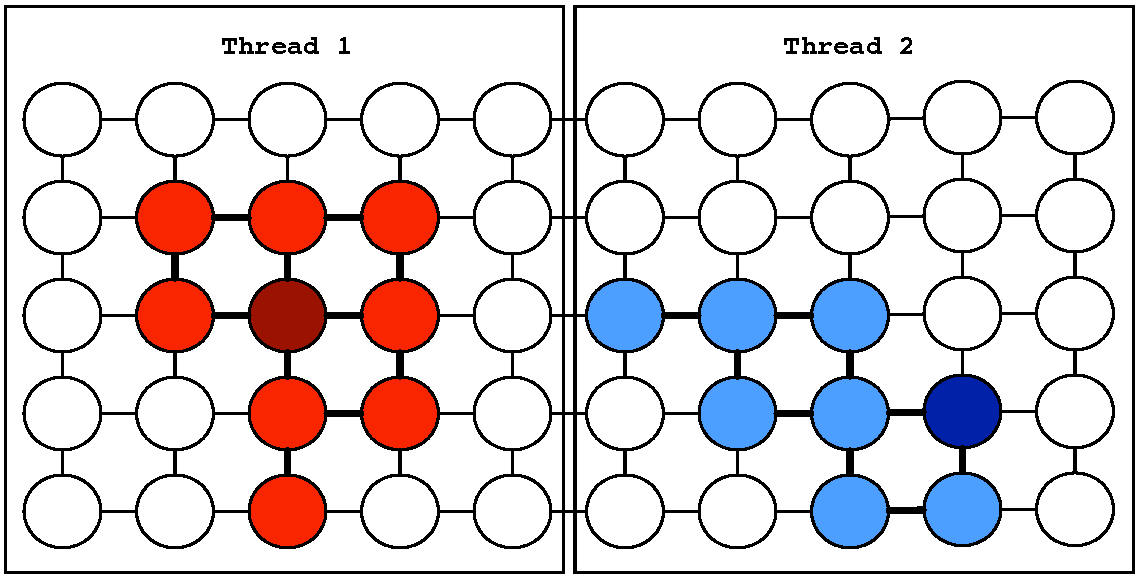
\includegraphics[width=0.7\linewidth]{figures/threads/splash_bp}
   \end{center}
   \caption{Creating splash trees using two threads. The graph is
      partitioned into two regions and each thread is able to build separate
   splash trees starting from the highest priority node.}
   \label{fig:threads:splash_bp}
\end{figure}

The LM implementation for SBP is shown in Fig.~\ref{code:threads:sbp}. First,
in lines \ref{line:threads:splash_part1}-\ref{line:threads:splash_part2}, we
partition the nodes into regions using \code{set-thread} and then we start the
creation of the first splash tree (line~\ref{line:threads:splash_first}) by
deriving \code{start-tree(T)}.  The remaining phases of the algorithm are
explained next.

\begin{figure}[!htb]
\begin{Verbatim}[numbers=left,commandchars=*\{\},fontsize=\codesize]
type list node tree.

type linear partitioning(thread, int). // Number of nodes to receive.
type linear start-tree(thread).
type linear new-tree(thread, tree, tree).
type linear expand-tree(thread, tree).
type linear first-phase(thread, tree, tree).
type linear second-phase(thread, tree).
type linear start(node).

start(A).
partitioning(T, @world / @threads). // Move @world/@threads nodes.

!coord(A, X, Y), start(A) // Moving this node.*label{line:threads:splash_part1}
   -o set-static(A), set-thread(A, grid(X, Y)).
just-moved(A), partitioning(T, Left) // Thread received another node.
   -o partitioning(T, Left - 1).
partitioning(T, 0) -o start-tree(T).*label{line:threads:splash_part2}*label{line:threads:splash_first}

start-tree(T),*label{line:threads:splash_building1} priority(A, P), P > 0.0 *hfill{} // Tree building
   -o priority(A, P), expand-tree(T, [A], []).*label{line:threads:splash_building2}
expand-tree(T, [A | All], Next)
   -o thread-id(A, Id),
      [collect => L ; | !edge(A, L), ~ L in All, ~ L in Next,*label{line:threads:splash_agg1} priority(L, P), P > 0.0,
         thread-id(L, Id2), Id1 = Id2 -o priority(L, P), thread-id(L, Id2) ->
         new-tree(T, [A | All],
            if len(All) + 1 >= maxnodes then [] else Next ++ L end)].*label{line:threads:splash_agg2}*label{line:threads:splash_next}

new-tree(T, [A | All], [])
   -o schedule-next(A), first-phase(T, reverse([A | All]), [A | All]).*label{line:threads:splash_first_phase}
new-tree(T, All, [B | Next])
   -o schedule-next(B), expand-tree(T, [B | All], Next).

first-phase(T, [A], [A]), running(T, A) *hfill{} // First phase
   -o running(T, A), update(A), remove-priority(A), start-tree(T).
first-phase(T, [A, B | Next], [A]), running(T, A)
   -o running(T, A), update(A), schedule-next(B), second-phase(T, [B | Next]).*label{line:threads:splash_first_update1}
first-phase(T, All, [A, B | Next]), running(T, A)
   -o running(T, A), update(A), schedule-next(B), first-phase(T, All, [B | Next]).*label{line:threads:splash_first_update2}

second-phase(T, [A]), running(T, A) *hfill{} // Second phase
   -o running(T, A), update(A), remove-priority(A), start-tree(T).*label{line:threads:splash_second_update1}
second-phase(T, [A, B | Next]), running(T, A)
   -o running(T, A), update(A), schedule-next(B), second-phase(T, [B | Next]).*label{line:threads:splash_second_update2}
\end{Verbatim}

   \caption{LM code for the Splash Belief Propagation program.}
  \label{code:threads:sbp}
\end{figure}

\begin{description}

   \item[Tree building:] Starts after the rule in lines
      \ref{line:threads:splash_building1}-\ref{line:threads:splash_building2} is
      derived. Since the thread always picks the highest priority node, we start
      by adding that node to the list that represents the tree. In lines
      \ref{line:threads:splash_agg1}-\ref{line:threads:splash_agg2}, we use an
      aggregate to gather all the neighbor nodes that have a positive priority
      (due to a new belief update) and are in the same thread. Nodes are
      collected into list \code{L} and appended to list \code{Next}
      (line~\ref{line:threads:splash_next}).

   \item[First phase:] When the number of nodes in the tree reaches a certain
      limit, a \code{first-phase} is generated to update the beliefs of all
      nodes in the tree (line~\ref{line:threads:splash_first_phase}). As the
      nodes are updated, starting from the leaves and ending at the root, an
      \code{update} fact is derived to update the belief values
      (lines~\ref{line:threads:splash_first_update1}
      and~\ref{line:threads:splash_first_update2}).

   \item[Second phase:] Performs the computation of beliefs from the root to the
      leaves and the belief values are updated a second time
      (lines~\ref{line:threads:splash_second_update1}
      and~\ref{line:threads:splash_second_update2}).

\end{description}

SBP is also implemented in GraphLab~\cite{GraphLab2010}, a C++ framework for
writing machine learning algorithms. GraphLab provides the splash scheduler as
part of its framework. We measured the behavior of LBP and SBP for both LM and
GraphLab. Fig.~XXX shows that both systems have very similar behavior when using
a variable number of threads, but for higher number of threads and, in
particular, for more than 15 threads, LM shows better speedups than GraphLab. In
terms of running times, LM is, on average, 1.4 times slower than GraphLab,
although LM program code is more concise.


\section{Modeling the Operational Semantics in LM}
The introduction of thread-based facts allows for explicit parallelism in a
language that is purely implicit. This introduces issues when attempting to
prove the correctness of programs because the behavior of threads and the
scheduling strategy is now also part of the program logic. Some of this behavior
is hidden from programs because it is part of how coordination facts and thread
scheduling works on the virtual machine.

Consider the SBP program in Fig.~\ref{code:threads:sbp} where in
lines~\ref{line:threads:splash_part1}-\ref{line:threads:splash_part2} the graph
of nodes is partitioned into regions. In order to prove the correct
partitioning, we need to know how the VM initially randomly assigns nodes to
threads and also how coordination facts \code{set-thread} and \code{just-moved}
are used by the VM.  Fortunately, since linear logic is the foundation of LM, it
is possible to model the semantics of LM by using LM rules. In
Chapter~\ref{chapter:implementation}, we have seen that threads and nodes
transition between different states during execution and thus we are going to
model that. We first define the following node facts:

\begin{itemize}

   \item \code{inactive(node A)}: Fact present on nodes that are not currently
      running on a thread. Facts \code{running(T, A)} and \code{inactive(A)} are
      mutually exclusive.

   \item \code{owner(node A, thread T)}: Fact that indicates the current thread
      \code{T} that currently owns node \code{A}.

   \item \code{available-work(node A, bool F)}: Fact that indicates if node
      \code{A} has new facts to be processed.

\end{itemize}

In terms of thread facts we have the following:

\begin{itemize}
   \item \code{active(thread T)}: Fact exists if thread \code{T} is currently
      active.

   \item \code{idle(thread T)}: Fact exists if thread \code{T} is currently
      idle. Facts \code{idle(T)} and \code{active(T)} are mutually exclusive.
\end{itemize}

Figure~\ref{code:threads:modeling} presents how the operational semantics for a
given LM program is modeled using the LM language itself.

First, we define the initial facts: \code{owner(A, T)} on
line~\ref{line:threads:model_owner}, which assigns a node to a thread;
\code{available-work(A, F)} on line~\ref{line:threads:model_available}, where
\code{F = true} if node \code{A} has initial facts, otherwise \code{F = false};
\code{active(T)} on line~\ref{line:threads:model_active} to mark each thread as
\emph{active}; and \code{moving(A)} on line~\ref{line:threads:model_moving} so
that all nodes can move between threads.

Each program rule is translated as shown in
lines~\ref{line:threads:model_rule1}-\ref{line:threads:model_rule2}. The
original rule was \code{node-fact(A, Y), other-fact(A, B) -o remote-fact(B),
local-fact(A)}, so we have a local derivation of \code{local-fact(A)} and a
remote-derivation of \code{remote-fact(B)}. In the translation, we update
\code{available-work} of node \code{B} to \code{true} because there is a new
derivation for \code{B}. The fact \code{running(T, A)} is used to ensure that
thread \code{T} is running on node \code{A}. Note that for thread rules we do
not need to use \code{running(T, A)} on the rule's LHS and the thread running
the rule does not even need to have \code{active(T)}. This enforces the
non-deterministic semantics for thread rules.

After the program rules are translated, we have the rule in
lines~\ref{line:threads:model_drop_node1}-\ref{line:threads:model_drop_node2}
which forces thread \code{T} to stop running on node \code{A}. Here, we use the
coordination fact \code{default-priority} to update the priority of node
\code{A}. The thread's state switches to \code{idle(T)}, while the node's state
changes to \code{inactive(A)}. Note that this rule must appear after the
program's rules because the rule priorities are exploited in order to force
thread \code{T} to derive all the candidate rules for \code{A}.

If a thread is idle, then it is able to derive the rule in
lines~\ref{line:threads:model_next_node1}-\ref{line:threads:model_next_node2} in
order to select another node for execution. We use a \code{max} selector to
select the node \code{A} with the highest priority \code{Prio}. If there is such
node, the node changes to \code{running(T, A)} and thread \code{T} changes to
\code{active(T)}.

Finally, the rule in
lines~\ref{line:threads:model_steal1}-\ref{line:threads:model_steal2} allows for
threads to steal nodes owned by other threads. If a node is not currently being
executed (\code{inactive(A)}), can be moved (\code{moving(A)}), and is owned by
another thread \code{Other} (\code{owner(A, Other)}), then the thread owner is
updated, potentially allowing the previous rule to execute.

\begin{figure}[h!]
\begin{Verbatim}[numbers=left,fontsize=\codesize,commandchars=\\\#\&]
type linear running(thread, node). type linear inactive(node).
type linear priority(node, float). type linear default-priority(node, float).
type linear available-work(node, bool).
type linear active(thread).  type linear idle(thread).
type linear owner(node, thread).
type linear moving(node).

owner(A, T). // Initially node assignment.\label#line:threads:model_owner&
available-work(A, F). // Some nodes have available work.\label#line:threads:model_available&
moving(A). // All nodes can be stolen.\label#line:threads:model_moving&
active(T). // All threads are active.\label#line:threads:model_active&

// Program rules go here.\label#line:threads:model_rule1&
\underline#node-fact(A, Y)&,
\underline#other-fact(A, B)&,
running(T, A), available-work(B, _)
   -o \underline#remote-fact(B)&, \underline#local-fact(A)&,
      running(T, A),
      available-work(B, true).\label#line:threads:model_rule2&

// Switching to another node.\label#line:threads:model_drop_node1&
active(T), running(T, A), priority(A, Prio),
default-priority(A, DefPrio), available-work(A, T)
   -o inactive(A), priority(A, DefPrio),
      default-priority(A, DefPrio),
      available-work(A, false), idle(T).\label#line:threads:model_drop_node2&

// Select next node to be processed.\label#line:threads:model_next_node1&
[max => Prio |
   idle(T), owner(A, T),
   priority(A, Prio), available-work(A, true)]
   -o active(T), owner(A, T),
      running(T, A), available-work(A, false),
      priority(A, Prio).\label#line:threads:model_next_node2&

// Attempt to steal a node.\label#line:threads:model_steal1&
idle(T), !other-thread(T, Other)
owner(A, Other), inactive(A),
available-work(A, true),
moving(A)
   -o idle(T), owner(A, T), moving(A),
      inactive(A), available-work(A, true).\label#line:threads:model_steal2&
\end{Verbatim}
\caption{Modeling the operational semantics as a LM program.}
\label{code:threads:modeling}
\end{figure}

\subsection{Scheduling}

We now model several coordination facts presented in
Chapter~\ref{chapter:coordination} using LM rules. We focus on
\code{set-thread}, \code{set-priority}, \code{just-moved}, and
\code{schedule-next}. The rules are presented in
Fig.~\ref{code:threads:modeling_scheduling} and should be the highest priority
rules in LM programs.

We start with the axiom~\code{priority(A, initial-priority)} and
\code{default-priority(A, initial-priority)}
(lines~\ref{line:threads:model_prio} and~\ref{line:threads:model_defprio}) to
define the initial priorities of nodes. In line~\ref{line:threads:model_snext}
we have the rule for the \code{schedule-next} coordination fact, which simply
re-derives a \code{set-priority} but with an infinite priority. Fact
\code{set-priority} is processed in
lines~\ref{line:threads:model_set1}-\ref{line:threads:model_set2} by updating
the priority values in the \code{priority} facts. As explained in
Chapter~\ref{chapter:coordination}, only higher priorities are taken into
account.

For the \code{set-thread} coordination fact, we have
lines~\ref{line:threads:model_thread1}-\ref{line:threads:model_thread2}. The
first rule applies when the node is currently executing on some thread, forcing
the thread to stop executing the node and to derive \code{just-moved(A)}. In the
second rule, node \code{A} is not being executed and the \code{owner} fact is
simply updated to the new thread.

Note that the rules for updating the coordination sensing facts do not require
the \code{running} predicate in the rule's body, therefore it should not matter
which thread does the update as long as it is done. In the VM, the update is
always done by thread that derives the coordination fact for efficiency reasons.

\begin{figure}[h!]
\begin{Verbatim}[numbers=left,fontsize=\codesize,commandchars=\\\#\&]
type linear static(node).  type linear moving(node).
type linear set-priority(node, float).
type linear just-moved(node). type linear move-to-thread(node, thread).

// Priority facts.
priority(A, initial-priority).\label#line:threads:model_prio&
default-priority(A, initial-priority).\label#line:threads:model_defprio&

schedule-next(A) -o set-priority(A, +00).\label#line:threads:model_snext&

set-priority(A, P1), priority(A, P2), P2 < P1\label#line:threads:model_set1&
   -o priority(A, P1).

set-priority(A, P1), priority(A, P2), P2 >= P1
   -o priority(A, P2).\label#line:threads:model_set2&

running(T, A), set-thread(A, T),\label#line:threads:model_thread1&
available-work(A, _), moving(A)
   -o available-work(A, true),
      inactive(A), static(A),
      just-moved(A).

inactive(A), set-thread(A, T),
owner(A, TOld), moving(A),
available-work(A, _)
   -o static(A), owner(A, T), just-moved(A),
      available-work(A, true).\label#line:threads:model_thread2&
\end{Verbatim}
\caption{Modeling the operational semantics for coordination facts as a LM program.}
\label{code:threads:modeling_scheduling}
\end{figure}


\section{Related Work}
As already seen in the previous chapter, there are several programming models
such as Galois~\cite{nguyen11}, Elixir~\cite{Prountzos:2012:ESS:2384616.2384644}
and Halide~\cite{Ragan-Kelley:2013:HLC:2491956.2462176}
which allow the programmer to apply different scheduling policies to programs.
Unfortunately, these models only reason about the data or program being computed
and not about the parallel architecture.

In the logic programming community, there have been some attempts at exposing a
low level programming interface in Prolog programs to permit explicit programmer
control. An example is the proposal by Casas et
al.~\cite{Casas_towardshigh-level} which exposes execution primitives for
AND-parallelism, allowing for different scheduling policies. Compared to LM,
this approach offers a more fine grained control to parallelism but has limited
support for reasoning about thread state.


\section{Chapter Summary}

In this chapter, we have extended the LM language with a declarative mechanism
for reasoning about the underlying parallel architecture. LM programs can be
first written in a data-driven fashion and then optimized by reasoning about the
state of threads, enabling the move from implicit parallelism to explicit
parallelism. We have presented four programs that showcase the potential of the
new mechanism and several experimental results that validate our approach.




\chapter{Conclusions}

In this chapter, we summarize the main contributions of this thesis and suggest
several directions for further research.

\section{Main Contributions}

The goal of our thesis was to show the potential of using a forward-chaining
linear logic programming language to exploit parallelism in a declarative,
efficient and scalable way. For this, we designed and implemented LM, a
programming language suitable for writing concurrent algorithms over graph
data-structures. LM programs are composed of a set of inference rules that apply
over a database of logical facts. Concurrency is achieved by partitioning the
database across a graph data structures and forcing rule derivation to happen at
the node level. Since LM is based on linear logic, facts used in rules may be
retracted, making it possible for the programmer to declaratively manage
structured state.

We introduced coordination facts in LM to show that it is possible for the
programmer to change how programs are scheduled in order to improve program run
time and scalability. This is possible due to the existence of linear facts,
which make it possible for different scheduling decisions to have an effect on
program computation. Without them, a logic program would always compute the same
result.

We also introduced explicit parallelism in LM by adding support for thread
facts. Thread facts are facts stored at the thread level and allow the
programmer to write rules that reason about thread state. This opens new
opportunities for program optimization and improved parallelism because programs
are aware of the existence of threads. Furthermore, the availability of both
thread and coordination facts allows and is convenient for implementing more
sophisticated scheduling parallel algorithms.

We now highlight in more detail the main contributions of this dissertation:

\begin{description}
   \item[Structured State]

Since LM is based on linear logic, LM enables programs to manage state in a
structured manner. Due to the restriction over the inference rules, rules are
derived independently on different nodes of the graph data structure, which
makes it possible to run LM programs in parallel.

   \item[Implementation]

Writing efficient implementations of declarative languages is challenging,
especially when adding support for parallel execution. In this thesis, we have
shown a compilation strategy and memory layout organization for LM programs,
which allows programs to run less than one order of magnitude slower than
hand-written C++ programs. We also described how the LM runtime supports
multicore execution by partitioning the graph among threads. To the best of our
knowledge, LM is the fastest linear logic based programming language available.

\item[Semantics and Abstract Machine]

We showed how LM semantics are specified in order to allow concurrent
programs. We demonstrated how the language is based upon the sequent calculus of
linear logic and we specified a low level abstract machine that closely
resembles the real implementation. We also proved the soundness of the
abstract machine.

\item[Coordination]

We presented new coordination features that improve the expressive
power of the language by making coordination a first class programming construct
that is semantically equivalent to regular computation. In turn, this allows the
programmer to specify how declarative programs are scheduled by the runtime
system, therefore improving overall run time and scalability.

Coordination facts are divided into scheduling and partitioning facts.
Scheduling facts change how nodes are scheduled by the system while partitioning
facts change how nodes are assigned to threads and how they move between
threads. Both these two types of facts are divided into sensing facts (with
information about the state of the runtime system) and action facts (which
perform actions on the runtime system). The interplay between regular facts,
sensing facts and action facts results in faster execution time and improved
parallelism because regular facts affect how action facts are derived and,
conversely, action facts may affect which regular facts are derived.

The coordination facts do not affect the correctness of programs and are well
integrated into proofs since they do not change how rules are scheduled but how
nodes are scheduled during execution.

\item[Explicit Parallelism]

We also introduced the concept of thread facts, which enable LM programs to
exploit the underlying architecture by making it possible to reason about the
state of threads. Thread facts allow the programmer to escape the default
implicit parallelism of LM and allows the implementation of structured
scheduling algorithms which require explicit communication between threads.
To the best of our knowledge, this is the first time that such paradigm
is available in a logic programming language and we are not aware of competing
systems that allow the programmer to reason directly about thread state in a
structured fashion.

\item[Experimentation]

We compared LM sequential and multithreaded execution to hand-written sequential
C++ programs and against frameworks such as GraphLab and Ligra. We showed how
well the LM runtime is able to scale using different programs and datasets. We
measured the run time, scalability and memory usage effects of using
coordination facts and their overheads. For thread facts, we analyzed different
applications and measured the performance improvements of using explicit
parallelism.

In our experiments, we noted that the memory layout of applications, especially
the memory allocator, tends to have a significant effect on the overall
performance. In modern architectures, good memory locality is as important as
having efficient algorithms and in LM this is no different.
We experimented with two allocators to analyze how
performance and scalability may be affected by using different strategies. It is
our belief that it is important to focus on faster sequential execution at the
expense of scalability in order to make declarative parallel languages more
competitive with sequential programs written in languages such as C++.

\end{description}

\section{Future Work}

While much progress has been achieved with this thesis, many new research
avenues have been opened with this work. We now enumerate further research goals
that should be interesting to pursue.

\begin{description}
   \item[Faster Implementation]

LM is still not competitive enough to replace efficient parallel frameworks such
as Ligra. LM is a programming language on its own right and thus requires more
engineering effort to be competitive with frameworks implemented in languages
such as C or C++. Better compilation and runtime systems will be required in
order to reduce the overhead even further, especially as it relates to memory
usage.

Aggressive code analysis should be employed to prove invariants about predicates
and introduce more specialized data structures for storing logical facts. The
goal should be to recover more of the \emph{imperative flavor} that is present
in linear logic programs in order to make them more efficient. The restrictions
of LM rules that make concurrency possible makes this task harder since there is
an inherent tension between concurrency and execution speed since concurrency
implies communication. However, local node computation has still some room for
improvement.

\item[Provability]

We need automated tools for reasoning about correctness and termination of
programs. While we have shown that writing informal proofs is relatively easy
because programs tend to be small, automated proof systems will increase the
faith that programs will work correctly. Ideally, the programmer should be able
to write invariants about the program and the compiler should be able to prove
if such invariants are or are not being met with the given inference rules.

\item[Expressiveness]

Although LM programs are expressive, some work must be done in order to reduce
the restrictions on LM rules and allow for more programmer freedom.  LM
currently only allows rules where the LHS refers to the same node, however, it
should be possible to allow rules that use facts from different nodes. The use
of linear logic facts makes this hard because we need to ensure that a linear
fact is used only once, therefore the compiler should generate code to enforce
this, probably through the use of transactions. In the CHR community, Lam et
al.~\cite{Lam:2013:DEC:2505879.2505892} have developed an encoding for
distributed rules using at most one immediate neighbor into rules that run
locally. It should be relatively straightforward to provide a similar encoding
for LM and then assess how performance is affected by such encoding.

\item[Implicit and Explicit Parallelism] We need more applications that take
   advantage of the mixed parallelism that is available with thread facts. We
   feel that this paradigm needs to be further explored in order to make it
   possible to write new scheduling and parallel algorithms that could be
   compiled to efficient code in other application areas. Furthermore,
   mechanized proofs about such algorithms could then be automatic, improving
   the correctness and reliability of parallel algorithms.

\end{description}

\section{Final Remark}

We argue that our work makes LM the ideal framework for prototyping new
(correct) graph algorithms since LM programs tend to be relatively short and the
programmer only needs to reason about the state of the graph, without the need
to understand how the framework must be used to express the intended algorithms.
Furthermore, the addition of coordination facts and thread facts help the
programmer exploit the underlying parallel architecture in order to create
better programs that take advantage of those architectures without radically
changing the underlying parallel algorithm.  Finally, the good performance of
the LM system allows programs to run reasonably fast when executed on multicore
systems.



\appendix
\chapter{Sequent Calculus}\label{sec:fragment}

\[
\infer[\otimes R]
{\Psi ; \seqx{\Gamma}{\Delta, \Delta'}{A \otimes B}}
{\Psi ; \seqx{\Gamma}{\Delta}{A} & \seqx{\Gamma}{\Delta}{B}}
\tab
\infer[\otimes L]
{\Psi ;\seqx{\Gamma}{\Delta, A \otimes B}{C}}
{\Psi ; \seqx{\Gamma}{\Delta, A, B}{C}}
\]

\[
\infer[\lolli R]
{\Psi ; \seqx{\Gamma}{\Delta}{A \lolli B}}
{\Psi ; \seqx{\Gamma}{\Delta, A}{B}}
\tab
\infer[\lolli L]
{\seqx{\Gamma}{\Delta, \Delta', A \lolli B}{C}}
{\Psi ; \seqx{\Gamma}{\Delta}{A} &
   \Psi ; \seqx{\Gamma}{\Delta', B}{C}}
\]


\[
\infer[\bang R]
{\Psi ; \seqx{\Gamma}{\cdot}{\bang A}}
{\Psi ; \seqx{\Gamma}{\cdot}{A}}
\tab
\infer[\bang L]
{\Psi ; \seqx{\Gamma}{\Delta, \bang A}{C}}
{\Psi ; \seqx{\Gamma, A}{\Delta}{C}}
\tab
\infer[\m{copy}]
{\Psi ; \seqx{\Gamma, A}{\Delta}{C}}
{\Psi ; \seqx{\Gamma, A}{\Delta, A}{C}}
\]

\[
\infer[\one R]
{\Psi ; \seqx{\Gamma}{\cdot}{\one}}
{}
\tab
\infer[\one L]
{\Psi ; \seqx{\Gamma}{\Delta, \one}{C}}
{\Psi ; \seqx{\Gamma}{\Delta}{C}}
\]

\[
\infer[\forall R]
{\Psi ; \seqx{\Gamma}{\Delta}{\forall_{n:\tau}. A}}
{\Psi, m:\tau ; \seqx{\Gamma}{\Delta}{A\{m/n\}}}
\tab
\infer[\forall L]
{\Psi ; \seqx{\Gamma}{\Delta, \forall_{n:\tau}. A}{C}}
{\Psi \vdash M : \tau & \Psi ; \seqx{\Gamma}{\Delta, A\{M/n\}}{C}}
\]

\[
\infer[\exists R]
{\Psi ; \seqx{\Gamma}{\Delta}{\exists_{n: \tau}. A}}
{\Psi \vdash M : \tau &
   \Psi ; \seqx{\Gamma}{\Delta}{A \{M/n\}}}
\tab
\infer[\exists L]
{\Psi ; \seqx{\Gamma}{\Delta, \exists_{n:\tau}. A}{C}}
{\Psi, m:\tau ; \seqx{\Gamma}{\Delta, A\{m/n\}}{C}}
\]

\[
\infer[\itersname^* R]
{\Psi ; \seqx{\Gamma}{\Delta}{\iters{name}{\widehat{V}}}}
{\Psi ; \seqx{\Gamma}{\Delta}{\iter{name}{N}{\widehat{V}}}}
\tab
\infer[\itersname^* L]
{\Psi ; \seqx{\Gamma}{\Delta, \iters{name}{\widehat{V}}}{C}}
{\Psi ; \seqx{\Gamma}{\Delta, \iter{name}{N}{\widehat{V}}}{C}}
\]

\[
\infer[\itersname^N R]
{\Psi ; \seqx{\Gamma}{\Delta}{\iter{name}{N}{\widehat{V}}}}
{\Psi ; \seqx{\Gamma}{\Delta}{\forall_{\widehat{x}}. (A \widehat{x} \lolli B
      \otimes \iter{name}{N-1}{(\iterop{x}{V})}})}
\]
\[
\infer[\itersname^N L]
{\Psi ; \seqx{\Gamma}{\Delta, \iter{name}{N}{\widehat{V}}}{C}}
{\Psi ; \seqx{\Gamma}{\Delta, \forall_{\widehat{x}}. (A \widehat{x} \lolli B
      \otimes \iter{name}{N-1}{(\iterop{x}{V})})}{C}}
\]

\[
\infer[\itersname^0 R]
{\Psi ; \seqx{\Gamma}{\Delta}{\iter{name}{0}{\widehat{V}}}}
{\Psi ; \seqx{\Gamma}{\Delta}{(\lambda_{\widehat{x}}. A)\widehat{V}}}
\tab
\infer[\itersname^0 L]
{\Psi ; \seqx{\Gamma}{\Delta, \iter{name}{0}{\widehat{V}}}{C}}
{\Psi ; \seqx{\Gamma}{\Delta, (\lambda_{\widehat{x}}. A)\widehat{V}}{C}}
\]


\chapter{High Level Dynamic Semantics}\label{sec:hld}

\section{Step}

\[
\infer[\stepz]
{\begin{split}
   \stepz [\Gamma_1, \dotsc, \Gamma_i, \dotsc, \Gamma_n]&; [\Delta_1, \dotsc,
   \Delta_i, \dotsc, \Delta_n]; \Phi \\
   \Longrightarrow& \\ [\Gamma_1, \Gamma'_1, \dotsc, \Gamma_i,
   \Gamma'_i, \dotsc, \Gamma_n, \Gamma'_n]; & [\Delta_1, \Delta'_1, \dotsc, (\Delta_i -
         \Xi'), \Delta'_i, \dotsc, \Delta_n, \Delta'_n]
\end{split}
}
{\doz{\Gamma_i}{\Delta_i}{\Phi}{\Pi}{\Xi'}{\Gamma'_1, \dotsc,
   \Gamma'_n}{\Delta'_1, \dotsc, \Delta'_n}
}
\]


\section{Application}

\[
\infer[\az \m{rule}]
{\az \Gamma ; \Delta_1, \Delta_2 ; A \lolli B \rightarrow \Xi' ; \Delta' ; \Gamma'}
{\mz \Gamma ; \Delta_1 \rightarrow A & \dz \Gamma ; \Delta_2; \Delta_1; \cdot ; \cdot ; B \rightarrow \Xi' ; \Delta' ; \Gamma'}
\]

\[
\infer[\doz \m{rule}]
{\doz \Gamma ; \Delta ; R, \Phi \rightarrow \Xi' ; \Delta' ; \Gamma'}
{\az \Gamma ; \Delta ; R \rightarrow \Xi' ; \Delta' ; \Gamma'}
\]


\section{Match}

\[
\infer[\mz \one]
{\mz \Gamma; \cdot \rightarrow \one}
{}
\]
\[
\infer[\mz p]
{\mz \Gamma; p \rightarrow p}
{}
\tab
\infer[\mz \bang p]
{\mz \Gamma, p; \cdot \rightarrow \bang p}
{}
\]

\[
\infer[\mz \otimes]
{\mz \Gamma; \Delta_1, \Delta_2 \rightarrow A \otimes B}
{\mz \Gamma; \Delta_1 \rightarrow A & \mz \Gamma; \Delta_2 \rightarrow B}
\]


\section{Derivation}

\[
\infer[\dz p]
{\dz \Gamma ; \Delta ; \Xi ; \Gamma_1 ; \Delta_1 ; p, \Omega \rightarrow \Xi' ; \Delta' ; \Gamma'}
{\dz \Gamma ; \Delta ; \Xi ; \Gamma_1 ; p, \Delta_1 ; \Omega \rightarrow \Xi' ; \Delta' ; \Gamma'}
\]

\[
\infer[\dz \bang p]
{\dz \Gamma ; \Delta ; \Xi ; \Gamma_1 ; \Delta_1 ; \bang p, \Omega \rightarrow \Xi' ; \Delta' ; \Gamma'}
{\dz \Gamma ; \Delta ; \Xi ; \Gamma_1, p ; \Delta_1 ; \Omega \rightarrow \Xi' ; \Delta' ; \Gamma'}
\]

\[
\infer[\dz \otimes]
{\dz \Gamma ; \Delta ; \Xi ; \Gamma_1 ; \Delta_1 ; A \otimes B, \Omega \rightarrow \Xi' ; \Delta' ; \Gamma'}
{\dz \Gamma ; \Delta ; \Xi ; \Gamma_1 ; \Delta_1 ; A, B, \Omega \rightarrow \Xi' ; \Delta' ; \Gamma'}
\]

\[
\infer[\dz \one]
{\dz \Gamma ; \Delta ; \Xi ; \Gamma_1; \Delta_1 ; 1, \Omega \rightarrow \Xi' ; \Delta' ; \Gamma'}
{\dz \Gamma ; \Delta ; \Xi ; \Gamma_1; \Delta_1 ; \Omega \rightarrow \Xi' ; \Delta' ; \Gamma'}
\]

\[
\infer[\dz end]
{\dz \Gamma ; \Delta ; \Xi' ; \Gamma' ; \Delta' ; \cdot \rightarrow \Xi' ; \Delta' ; \Gamma'}
{}
\]

\[
\infer[\dz \m{agg}^*]
{\dz \Gamma ; \Delta ; \Xi ; \Gamma_1 ; \Delta_1 ; \aggsz{A}{B}{C}, \Omega
   \rightarrow \outsem}
{\dz \Gamma ; \Delta ; \Xi ; \Gamma_1 ; \Delta_1 ; \aggz{N}{A}{B}{C}{0}, \Omega
   \rightarrow \outsem}
\]

{\small
\[
\infer[\dz \m{agg}^N]
{\dz \Gamma ; \Delta ; \Xi ; \Gamma_1 ; \Delta_1 ; \aggz{N}{A}{B}{C}{V}, \Omega
   \rightarrow \outsem}
{\dz \Gamma ; \Delta ; \Xi ; \Gamma_1 ; \Delta_1 ; \aggunfold{N-1}{A}{B}{C}{V},
   \Omega \rightarrow \outsem}
\]
}

\[
\infer[\dz \m{agg}^0]
{\dz \Gamma ; \Delta ; \Xi ; \Gamma_1 ; \Delta_1 ; \aggz{0}{A}{B}{C}{V}, \Omega
   \rightarrow \outsem}
{\dz \Gamma ; \Delta ; \Xi ; \Gamma_1 ; \Delta_1 ; \aggunfoldz{C}{V}, \Omega
   \rightarrow \outsem}
\]

\[
\infer[\dz \lolli]
{\dz \Gamma ; \Delta_a, \Delta_b ; \Xi ; \Gamma_1 ; \Delta_1 ; A \lolli B,
   \Omega \rightarrow \outsem}
{\mz \Gamma ; \Delta_a \rightarrow A & \dz \Gamma ; \Delta_b ; \Xi, \Delta_a ;
   \Gamma_1 ; \Delta_1 ; B, \Omega \rightarrow \outsem}
\]



\chapter{Low Level Dynamic Semantics}\label{sec:lld}

%\section{Step}

%\[
\infer[\stepo]
{\begin{split}
\stepo [\Gamma_1, \dotsc, \Gamma_i, \dotsc, \Gamma_n] &; [\Delta_1, \dotsc,
   \Delta_i, \dotsc, \Delta_n];
   \Phi \\ \Longrightarrow& \\ [\Gamma_1, \Gamma'_1, \dotsc, \Gamma_i, \Gamma'_i,
   \dotsc,
   \Gamma_n, \Gamma'_n]; & [\Delta_1, \Delta'_1, \dotsc, (\Delta_i - \Xi'),
   \Delta'_i, \dotsc, \Delta_n, \Delta'_n]
\end{split}
}
{
   \doo \Gamma_i; \Delta_i; \Phi \rightarrow \Xi'; \Delta'_1, \dotsc, \Delta'_n;
   \Gamma'_1, \dotsc, \Gamma'_n
}
\]


\section{Application}

\input{lld/init}
\input{lld/fail}
\input{lld/open_rule}
\input{lld/init_rule}


\section{Match}


\begin{multline}
\transx{\matstateb{A \lolli B}{\rulestk}{\lstack{C}}{\Gamma}{\Delta, p_1,
\Delta''}{p(\widehat{x}),
   \Omega}{\Delta' \rightarrow \Omega'}{\Psi}}
{\matstateb{A \lolli B}{\rulestk}{\lframe{\Delta,
p_1}{\Delta''}{p(\widehat{x})}{\Omega; \m{extend}(\Psi, \theta)}{\Delta'}{\Omega'}, \lstack{C}}{\Gamma}{\Delta,
   \Delta''}{\Omega}{\Delta', p_1 \rightarrow \Omega' \otimes
      p(\widehat{x}\theta)}{\m{extend}(\Psi, \theta)}} \\
   \;\;\; (p_1,
   \Delta'' \prec p(\widehat{x}) \;\;\; \Delta \npreceq p(\widehat{x}))
   \tag{match p ok}
\end{multline}

\begin{align}
   \trans{\matstate{A \lolli
   B}{\rulestk}{\lstack{C}}{\Gamma}{\Delta}{p(\widehat{x}),
   \Omega}{\Delta' \rightarrow \Omega'}}
{\contstate{A \lolli B}{\rulestk}{\lstack{C}}{\Gamma}} \;\;\; (\Delta \npreceq
p(\widehat{x})) \tag{match p fail}
\end{align}

\begin{align}
\trans{\matstate{A \lolli B}{\rulestk}{\lstack{C}}{\Gamma}{\Delta}{\bang p,
   \Omega}{\Delta' \rightarrow \Omega'}}
{\matstate{A \lolli B}{\rulestk}{\pframe{\Gamma''}{\Delta}{\bang
   p}{\Omega}{\Delta'}{\Omega'}, \lstack{C}}{\Gamma, p_1,
      \Gamma''}{\Delta}{\Omega}{\Delta' \rightarrow \Omega' \otimes \bang p}}
      \;\;\; (\bang p_1, \Gamma'' \prec \bang p) \tag{match \bang p ok}
\end{align}

\begin{align}
\trans{\matstate{A \lolli B}{\rulestk}{\lstack{C}}{\Gamma}{\Delta}{\bang p,
   \Omega}{\Delta' \rightarrow \Omega'}}
{\contstate{A \lolli B}{\rulestk}{\lstack{C}}{\Gamma}} \;\;\; (\Gamma \npreceq
      \bang p) \tag{match \bang p fail}
\end{align}


\begin{align}
\trans{\matstate{A \lolli B}{\rulestk}{\lstack{C}}{\Gamma}{\Delta}{\one,
   \Omega}{\Delta' \rightarrow \Omega'}}
{\matstate{A \lolli B}{\rulestk}{\lstack{C}}{\Gamma}{\Delta}{\Omega}{\Delta'
   \rightarrow \Omega'}} \tag{match $\one$}
\end{align}

\begin{align}
\trans{\matstate{A \lolli B}{\rulestk}{\lstack{C}}{\Gamma}{\Delta}{X \otimes Y,
   \Omega}{\Delta' \rightarrow \Omega'}}
{\matstate{A \lolli B}{\rulestk}{\lstack{C}}{\Gamma}{\Delta}{X, Y,
   \Omega}{\Delta' \rightarrow \Omega'}} \tag{match $\otimes$}
\end{align}

\begin{align}
\trans{\matstate{A \lolli
   B}{\rulestk}{\lstack{C}}{\Gamma}{\Delta}{\cdot}{\Delta' \rightarrow \Omega'}}
{
   \derstatex{\Gamma}{\Delta}{\Delta'}{\cdot}{\cdot}{B}
} \tag{match end}
\end{align}


\section{Continuation}
\begin{align}
\trans{\contstate{A \lolli B}{\rulestk}{\lframe{\Delta}{p_2,
   \Delta''}{p}{\Omega}{\Delta'}{\Omega'}, \lstack{C}}{\Gamma}}
{
   \matstate{A \lolli B}{\rulestk}{\lframe{\Delta,
      p_2}{\Delta''}{p}{\Omega}{\Delta'}{\Omega'},
   \lstack{C}}{\Gamma}{\Delta}{\Omega}{\Delta', p_2 \rightarrow \Omega' \otimes p}}
   \tag{next p}
\end{align}

\begin{align}
\trans{\contstate{A \lolli
   B}{\rulestk}{\lframe{\Delta}{\cdot}{p}{\Omega}{\Delta'}{\Omega'},
      \lstack{C}}{\Gamma}}
{
   \contstate{A \lolli B}{\rulestk}{\lstack{C}}{\Gamma}} \tag{next frame}
\end{align}

\[
\infer[\cont \bang p~\m{next}]
{\cont [p_1, \Gamma'; \Delta; \bang p, \Omega; \Xi; \Lambda; \Upsilon], C; H; R; \Gamma \rightarrow \Xi'; \Delta'; \Gamma'}
{\mo \Gamma; \Delta; \Xi; \Omega; H; [\Gamma'; \Delta; \bang p, \Omega; \Xi; \Lambda; \Upsilon], C; R \rightarrow \Xi'; \Delta'; \Gamma'}
\]

\[
\infer[\cont \bang p~\m{no~more}]
{\cont [\cdot; \Delta; \bang p, \Omega; \Xi; \Lambda; \Upsilon], C; H; R; \Gamma \rightarrow \Xi'; \Delta'; \Gamma'}
{\cont C; H; R; \Gamma \rightarrow \Xi'; \Delta'; \Gamma'}
\]

\begin{align}
\trans{\contstate{A \lolli B}{(\Delta; \Phi)}{\cdot}{\Gamma}}
   {\dostate{\Delta}{\Phi}{\Gamma}{\Pi}} \tag{rule fail}
\end{align}


\section{Derivation}
\[
\infer[\done p]
{\done \Gamma ; \Delta; \Xi; \Gamma_1 ; \Delta_1; p, \Omega \rightarrow \outsem}
{\done \Gamma ; \Delta; \Xi; \Gamma_1 ; p, \Delta_1; \Omega \rightarrow \outsem}
\tab
\infer[\done \bang p]
{\done \Gamma ; \Delta ; \Xi; \Gamma_1 ; \Delta_1; \bang p, \Omega \rightarrow
   \outsem}
{\done \Gamma ; \Delta ; \Xi; \Gamma_1, p; \Delta_1; \Omega \rightarrow \outsem}
\]

\[
\infer[\done 1]
{\done \Gamma; \Delta; \Xi; \Gamma_1 ; \Delta_1; 1, \Omega \rightarrow \outsem}
{\done \Gamma; \Delta; \Xi; \Gamma_1 ; \Delta_1; \Omega \rightarrow \outsem}
\tab
\infer[\done \otimes]
{\done \Gamma ; \Delta; \Xi; \Gamma_1; \Delta_1; A \otimes B, \Omega \rightarrow
   \outsem}
{\done \Gamma ; \Delta; \Xi; \Gamma_1; \Delta_1; A, B, \Omega \rightarrow
   \outsem}
\]

\[
\infer[\done \m{agg}]
{\done \Gamma; \Delta ; \Xi; \Gamma_1; \Delta_1; \aggsz{A}{B}{C}, \Omega
   \rightarrow \outsem}
{\ma \Gamma; \Delta; \Xi; \Gamma_1; \Delta_1; \cdot; A ; \cdot; \cdot;
   \aggsz{A}{B}{C}; \Omega; \Delta; \cdot \rightarrow \outsem}
\]

\begin{align}
\trans{\derstatex{\Gamma}{\Delta}{\Xi}{\Gamma_1}{\Delta_1}{\cdot}}
{\finalstate{\Xi}{\Gamma_1}{\Delta_1}} \tag{rule finished}
\end{align}


\section{Aggregates}
\subsection{Match}

\begin{multline}
\transx{
   \matstatea{\deltan}{\lstack{C};
      \lstack{P}}{\Gamma}{\Delta, p_1, \Delta''}{p, \Omega}{\Delta' \rightarrow
         \Omega'}{\Sigma}
}
{
   \matstatea{\deltan}{\lframe{\Delta,
   p_1}{\Delta''}{p}{\Omega}{\Delta'}{\Omega'}, \lstack{C}; \lstack{P}}{\Gamma}{\Delta,
      \Delta''}{\Omega}{\Delta', p \rightarrow \Omega' \otimes
      p}{\Sigma}\tag{agg match p ok}
}
\end{multline}

\[
\trans{
   \matstatea{\deltan}{\lstack{C}; \lstack{P}}{\Gamma}{\Delta}{p,
      \Omega}{\Delta' \rightarrow \Omega'}{\Sigma}
}
{
   \contstatea{\deltan}{\lstack{C} ; \lstack{P}}{\Gamma}{\Sigma}
}\tag{agg match p fail}
\]



\[
\trans{
   \matstatea{\Delta_N}{\cdot;
      \lstack{P}}{\Gamma, p_1, \Gamma''}{\Delta}{\bang p, \Omega}{\Delta' \rightarrow
         \Omega'}{\Sigma}
}
{
   \matstatea{\Delta_N}{\cdot; \pframe{\Gamma''}{\Delta}{\bang
   p}{\Omega}{\Delta'}{\Omega'}, \lstack{P}}{\Gamma, p_1, \Gamma''}{\Delta}{\Omega}
   {\Delta' \rightarrow \Omega' \otimes \bang p}{\Sigma}
}
\]

\[
\trans{
   \matstatea{\Delta_N}{\lstack{C};
      \lstack{P}}{\Gamma, p_1, \Gamma''}{\Delta}{\bang p, \Omega}{\Delta' \rightarrow
         \Omega'}{\Sigma}
}
{
   \matstatea{\Delta_N}{\pframe{\Gamma''}{\Delta}{\bang
   p}{\Omega}{\Delta'}{\Omega'}, \lstack{C} ; \lstack{P}}{\Gamma, p_1, \Gamma''}{\Delta}{\Omega}
   {\Delta' \rightarrow \Omega' \otimes \bang p}{\Sigma}
}
\]


\[
\trans{
   \matstatea{\Delta_N}{\lstack{C}; \lstack{P}}{\Gamma}{\Delta}{\bang p,
      \Omega}{\Delta' \rightarrow \Omega'}{\Sigma}
}
{
   \contstatea{\Delta_N}{\lstack{C} ; \lstack{P}}{\Gamma}{\Sigma}
}
\]



\begin{multline}
\transx{
   \matstatea{\deltan}{\lstack{C};
      \lstack{P}}{\Gamma}{\Delta}{X \otimes Y, \Omega}{\Delta' \rightarrow
         \Omega'}{\Sigma}
}
{
   \matstatea{\deltan}{\lstack{C};
      \lstack{P}}{\Gamma}{\Delta}{X, Y, \Omega}{\Delta' \rightarrow
         \Omega'}{\Sigma}
} \tag{agg match $\otimes$}
\end{multline}

\begin{multline}
\transx{
   \matstatea{\deltan}{\lstack{C};
      \lstack{P}}{\Gamma}{\Delta}{\one, \Omega}{\Delta' \rightarrow
         \Omega'}{\Sigma}
}
{
   \matstatea{\deltan}{\lstack{C};
      \lstack{P}}{\Gamma}{\Delta}{\Omega}{\Delta' \rightarrow
         \Omega'}{\Sigma}
      } \tag{agg match $\one$}
\end{multline}

\subsection{Stack Transformation}

{\tiny
\[
\infer[\fixa ~\m{end~linear}]
{\fixa \Gamma; \Xi_N; \Gamma_{N1}; \Delta_{N1}; \Xi; (\Delta_x; \Delta''; \cdot;
      p; \Omega; \cdot; \Upsilon); P;  \aggsz{A}{B}{C}; \Omega_N; \Delta_N; T \rightarrow \Xi'; \Delta'; \Gamma'}
{\begin{split}\strans &\Xi; P; P' \\ \da \Gamma; \Xi_N, \Xi; \Gamma_{N1};
   \Delta_{N1}; B; (\Delta_x - \Xi; \Delta'' - \Xi; \cdot;& p; \Omega; \cdot;
         \Upsilon) ; P' ; \aggsz{A}{B}{C}; \Omega_N; (\Delta_N - \Xi); T &\rightarrow \Xi'; \Delta'; \Gamma'\end{split}}
\]
}

\[
\infer[\fixa \m{more}]
{\fixa \Gamma; \Xi_N; \Gamma_{N1}; \Delta_{N1}; \Xi; \_, X, C; P; AG; \Omega_N; \Delta_N; T \rightarrow \Xi'; \Delta'; \Gamma'}
{\fixa \Gamma; \Xi_N; \Gamma_{N1}; \Delta_{N1}; \Xi; X, C; P; AG; \Omega_N; \Delta_N; T \rightarrow \Xi'; \Delta'; \Gamma'}
\]

{\footnotesize
\[
\infer[\fixa \m{end~empty}]
{\fixa \Gamma; \Xi_N; \Gamma_{N1}; \Delta_{N1}; \Xi; \cdot; P; \aggsz{A}{B}{C}; \Omega_N; \Delta_N; T \rightarrow \Xi'; \Delta'; \Gamma'}
{\begin{split}\strans &\Xi; P; P' \\ \da \Gamma; \Xi_N, \Xi; \Gamma_{N1};
   \Delta_{N1}; B; \cdot ; P' ; &\aggsz{A}{B}{C}; \Omega_N; (\Delta_N - \Xi); T &\rightarrow \Xi'; \Delta'; \Gamma'\end{split}}
\]
}

\subsection{Backtracking}

\begin{multline}
\transx{
   \contstatea{\deltan}{\lframe{\Delta}{p_1, \Delta''}{p}{\Omega}{\Delta'}{\Omega'}, \lstack{C} ; \lstack{P}}{\Gamma}{\Sigma}
}
{
   \matstatea{\deltan}{\lframe{\Delta,
      p_1}{\Delta''}{p}{\Omega}{\Delta'}{\Omega'}, \lstack{C}; \lstack{P}}{\Gamma}{\Delta}{p,
      \Omega}{\Delta', p_1 \rightarrow \Omega' \otimes p}{\Sigma}
} \tag{agg next p $\lstack{C}$}
\end{multline}

\begin{multline}
\transx{
   \contstatea{\deltan}{\pframe{p_1, \Gamma''}{\Delta}{\bang
   p}{\Omega}{\Delta'}{\Omega'}, \lstack{C} ; \lstack{P}}{\Gamma}{\Sigma}
}
{
   \matstatea{\deltan}{\pframe{\Gamma''}{\Delta}{\bang p}
      {\Omega}{\Delta'}{\Omega'}, \lstack{C}; \lstack{P}}{\Gamma}{\Delta}{p,
      \Omega}{\Delta' \rightarrow \Omega' \otimes \bang p}{\Sigma}
} \tag{agg next \bang p $\lstack{C}$}
\end{multline}

\[
\trans{
   \contstatea{\deltan}{\lframe{\Delta}{\cdot}{p}{\Omega}{\Delta'}{\Omega'}, \lstack{C} ; \lstack{P}}{\Gamma}{\Sigma}
}
{
   \contstatea{\deltan}{\lstack{C} ; \lstack{P}}{\Gamma}{\Sigma}
} \tag{agg  next frame $\lstack{C}$}
\]

\[
\trans{
   \contstatea{\deltan}{\pframe{\cdot}{\Delta}{\bang
   p}{\Omega}{\Delta'}{\Omega'}, \lstack{C} ; \lstack{P}}{\Gamma}{\Sigma}
}
{
   \contstatea{\deltan}{\lstack{C} ; \lstack{P}}{\Gamma}{\Sigma}
} \tag{agg next \bang frame $\lstack{C}$}
\]

\[
\infer[\conta{AG} \m{next}~\lstack{P}~\bang p]
{\conta{AG} \Gamma; \Delta_N; \Xi_N; \Gamma_{N1}; \Delta_{N1}; \cdot; f, \lstack{P}; \Omega_N; \Sigma \rightarrow \outsem}
{\begin{gathered}
   f = [p_1, \Gamma'; \Delta_N; \cdot; \bang p; \Omega; \cdot; \Upsilon] \\
   f' = [\Gamma'; \Delta_N; \cdot; \bang p; \Omega; \cdot; \Upsilon] \\
   \ma{AG} \Gamma; \Delta_N; \Xi_N; \Gamma_{N1}; \Delta_{N1}; \cdot; \Omega; \cdot;
      f', \lstack{P}; \Omega_N; \Delta_N; \Sigma \rightarrow \outsem
 \end{gathered}
}
\]

\[
\infer[\conta{AG} \m{next}~\lstack{P}~\m{empty}~\bang p]
{\conta{AG} \Gamma; \Delta_N; \Xi_N; \Gamma_{N1}; \Delta_{N1}; \cdot; f, \lstack{P}; \Omega_N; \Sigma
   \rightarrow \outsem}
{\begin{gathered}
   f =  [\cdot; \Delta_N; \cdot; \bang p; \Omega; \cdot; \Upsilon] \\
   \conta{AG} \Gamma; \Delta_N; \Xi_N; \Gamma_{N1}; \Delta_{N1}; \cdot; \lstack{P};
      \Omega_N; \Sigma \rightarrow \outsem
 \end{gathered}
}
\]

\[
\infer[\conta{\aggsz{A}{B}{C}} \m{end}]
{\conta{\aggsz{A}{B}{C}} \Gamma; \Delta_N; \Xi_N; \Gamma_{N1}; \Delta_{N1}; \cdot; \cdot;
   \Omega; \Sigma \rightarrow \outsem}
{\done \Gamma; \Delta_N; \Xi_N; \Gamma_{N1}; \Delta_{N1}; (\lambda x. C
      x)\Sigma,
   \Omega \rightarrow \outsem}
\]

\subsection{Derivation}
\[
\infer[\da{AG} p]
{\da{AG} \Gamma; \Delta_N; \Xi_N; \Gamma_1; \Delta_1; p, \Omega; \lstack{C}; \lstack{P}; \Omega_N;
   \Sigma \rightarrow \outsem}
{\da{AG} \Gamma; \Delta_N; \Xi_N; \Gamma_1; \Delta_1, p; \Omega; \lstack{C}; \lstack{P}; \Omega_N;
   \Sigma \rightarrow \outsem}
\]

\[
\infer[\da{AG} \bang p]
{\da{AG} \Gamma; \Delta_N; \Xi_N; \Gamma_1; \Delta_1; \bang p, \Omega; \lstack{C};
   \lstack{P}; \Omega_N; \Sigma \rightarrow \outsem}
{\da{AG} \Gamma; \Delta_N; \Xi_N; \Gamma_1, p; \Delta_1; \Omega; \lstack{C}; \lstack{P}; \Omega_N;
   \Sigma \rightarrow \outsem}
\]

\[
\infer[\da{AG} \otimes]
{\da{AG} \Gamma; \Delta_N; \Xi_N; \Gamma_1; \Delta_1; A \otimes B, \Omega; \lstack{C}; \lstack{P}; \Omega_N;
   \Sigma \rightarrow \outsem}
{\da{AG} \Gamma; \Delta_N; \Xi_N; \Gamma_1; \Delta_1; A, B, \Omega; \lstack{C}; \lstack{P}; \Omega_N;
   \Sigma \rightarrow \outsem}
\]

\[
\infer[\da{AG} \m{end}]
{\da{AG} \Gamma; \Delta_N; \Xi_N; \Gamma_1; \Delta_1; \cdot; \lstack{C}; \lstack{P}; \Omega_N;
   \Sigma \rightarrow \outsem}
{\conta{AG} \Gamma; \Delta_N; \Xi_N; \Gamma_1; \Delta_1; \lstack{C}; \lstack{P}; \Omega_N; \Sigma
   \rightarrow \outsem}
\]




\chapter{LM Directives}

In this section, we list all the extra-logical directives available in LM
programs.


\begin{itemize}

   \item \texttt{priority @order ORDER} (\texttt{ORDER} can be either \code{asc}
      or \code{desc}): Defines if priorities are to be selected by the smallest
      or the greatest value, respectively.

   \item \texttt{priority @default P}: Informs the runtime system that all nodes
      must start with default priority \code{P}. Alternatively, the programmer can define a
      \texttt{set-default-priority(A, P)} fact.

   \item \texttt{priority @base P}: Informs the runtime system that the
      \emph{base priority} should be \code{P}. The base priority is, by default,
      0 when the priority ordering is \code{desc} and $+\infty$ when the ordering
      is \code{asc} and represents the smallest priority value possible.

   \item \texttt{priority @initial P}: Informs the runtime system that all nodes
   must start with temporary priority \code{P}. Alternatively, the programmer can define an
      \texttt{set-priority(A, P)} fact. The default is value is the one defined
      as the \emph{base priority}.

\end{itemize}


\begin{itemize}
   \item \code{index pred/arg}: Informs the compiler that predicate \code{pred}
      should be indexed by the argument \code{arg} (number). The runtime system
      will use hash tree data structures for facts of this predicate indexed by
      the requested argument.
\end{itemize}


\chapter{Intermediate Representation}\label{appendix:vm}
In this appendix, we present the instructions implemented by our virtual
machine. We consider that the machine has an arbitrary number of registers (or
variables) that can be assigned to values or facts and a database of facts
indexed by program predicates.

\paragraph{Values}\label{appendix:vm:values} Values can be assigned to registers or to fact arguments
which are stored in the database. The following values are allowed:

\begin{itemize}
      \item Boolean values;
      \item Integer numbers;
      \item Floating point numbers;
      \item Node pointers;
      \item Thread pointers;
      \item String pointers;
      \item List pointers;
      \item Array pointers;
\end{itemize}

\section{Iteration Instructions}

The iteration instructions perform searches on the database of facts. When
inferring a rule, each iteration instruction iterates over a predicate in the
body of the rule in order to derive all combinations of facts that match the
rule.

\paragraph{Match Object} Every instruction points to a \code{match} object that
filters the facts from the database. The object maps argument indexes to value
templates. Value templates include the values described
in~\ref{appendix:vm:values} and the following variable templates:

\begin{itemize}
      \item Register: fact argument must equal to the value stored in the
         register;
      \item Fact argument: fact argument must be equal to the value stored in
         another fact argument;
      \item List template: describes the structure of a list, namely, the head
         and tail value template;
\end{itemize}

\paragraph{Iteration} Each iteration instruction contains the \code{body}, a list of instructions
that must be executed for each fact found in the database. The \code{body} also
returns a status indicating whether rule inference was successful or not.

\begin{itemize}
   \item \code{persistent iterate [pred : predicate, dest : register, m : match, body : instructions]}

   Iterate over persistent facts with the predicate \code{pred} that match
   \code{m}. For each iteration, we assign \code{dest} the next candidate fact
   and execute instructions \code{body}.

   \item \code{linear iterate [pred: predicate, dest : register, m : match, body : instructions]}

   Same as before but iterate over linear facts.

   \item \code{reuse linear iterate [pred: predicate, dest : register, m :
      match, body : instructions]}

   Iterates over linear facts but, if the rule has been successful, it does not
   remove the linear fact stored in \code{dest} since the same fact has been
   re-derived in the head of the rule.

\end{itemize}

\subsection{Return Instructions}

Return instructions terminate the current execution flow and force the machine
to backtrack to a previous state. In most cases, they are the return values used by iterate
instructions and force the iterate instruction to use the next candidate fact.

\begin{itemize}
   \item \code{return}

      Return without return value. Used at the end of rules to complete rule
      inference or in rules where a higher priority rule is available.

   \item \code{return derived}

      The rule was successfully derived.

   \item \code{return next}

      The matching has failed and the iterate instruction must use the next
      candidate fact.

\end{itemize}

\section{Conditional Instructions} Conditional instructions are used to
conditionally execute certain instructions.

\begin{itemize}
   \item \code{if [reg : register, body : instructions]}

   If the boolean value stored in \code{reg} is true then execute \code{body}.

   \item \code{if [reg : register, body1 : instructions, body2 : instructions]}

   If the boolean value stored in \code{reg} is true then execute \code{body1},
   otherwise execute \code{body2}.

   \item \code{jump [offset : integer]}

   Used as a goto at the end of \code{body1} in the instruction above. Jumps a
   certain number of instructions.

\end{itemize}

\section{Arithmetic and Boolean Instructions}

We briefly describe the most important arithmetic and boolean instructions.

\paragraph{Operations}

Available operations are as follows:

\begin{itemize}
   \item Addition \code{+};
   \item Subtraction \code{-};
   \item Multiplication \code{*};
   \item Division \code{/};
   \item Integer remainder \code{\%};
   \item Equality \code{=};
   \item Inequality \code{<>};
   \item Greater \code{>};
   \item Greater or equal \code{>=};
   \item Lesser \code{<};
   \item Lesser or equal \code{<=};
   \item Logical or \code{or};
   \item Logical and \code{and};
\end{itemize}

\paragraph{Instructions}

These operations are used as follows:

\begin{itemize}
   \item \code{test nil [reg : register, dest : register]}

   If the list stored in \code{reg} is null then set \code{dest} as \code{true}.

   \item \code{not [reg : register, dest : register]}

   Perform a boolean \code{not} operation.

   \item \code{int op [op1 : register, op2 : register, dest : register]}

   Perform an binary arithmetic operation on two integer numbers \code{op1} and
   \code{op2} and store result in \code{dest}. Operations include: \code{+},
   \code{-}, \code{*}, \code{/}, \code{\%}, \code{=}, \code{<>}, \code{<}, \code{<=},
   \code{>=}, and \code{>}.

   \item \code{float op [op1 : register, op2 : register, dest : register]}

   Perform an binary arithmetic operation on two floating point numbers \code{op1} and
   \code{op2} and store result in \code{dest}. Operations include: \code{+},
   \code{-}, \code{*}, \code{/}, \code{=}, \code{<>}, \code{<}, \code{<=},
   \code{>=}, and \code{>}.

   \item \code{node op [op1 : register, op2 : register, dest : register]}

   Perform an operation on two node addresses \code{op1} and
   \code{op2} and store result in \code{dest}. Operations include: \code{=} and
   \code{<>}.

   \item \code{thread op [op1 : register, op2 : register, dest : register]}

   Perform an operation on two thread addresses \code{op1} and
   \code{op2} and store result in \code{dest}. Operations include: \code{=} and
   \code{<>}.

   \item \code{[bool op [op1 : register, op2 : register, dest : register]}

   Perform an operation on two boolean values \code{op1} and
   \code{op2} and store result in \code{dest}. Operations include: \code{=} and
   \code{<>}, \code{and} and \code{or}.

\end{itemize}

\section{Data Instructions}

Data instructions include instructions which move values between registers and fact arguments and
instructions which call external functions written in C++ code.

\begin{itemize}
   \item \code{move-value-to-reg [val : value, reg : register]}

      Moves any value presented in~\ref{appendix:vm:values} to register \code{reg}.

   \item \code{move-arg-to-reg [fact : register, arg : integer, reg : register]}

      Moves the $\mathtt{arg}^{th}$ argument of fact stored in \code{fact} to
      register \code{reg}.

   \item \code{move-reg-to-arg [reg : register, fact : register, arg : integer]}

      Moves the value stored in \code{reg} to the $\mathtt{arg}^{th}$ argument of
      fact stored in \code{fact}.

   \item \code{call [id : integer, gc : boolean, dest : register, n : integer, arg1 :
      register, arg2 : register, ...]}

      Call external function with number \code{id} with \code{n} arguments
      \code{arg1} up to \code{argn} and store the return value in \code{dest}.
      If \code{gc} is \code{true} then garbage collect the return value at the
      end of the rule.

\end{itemize}

\section{List Instructions}

List instructions manipulate and access list addresses.

\begin{itemize}
   \item \code{cons [head : register, tail : register, gc : boolean, dest : register]}

      Create a new list and store its address in \code{dest}. The value of
      \code{tail} must be a list address or a null list. If \code{gc} is
      \code{true} then the list must be garbage collected after the rule
      executes.

   \item \code{head [ls : register, dest : register]}

   Retrieve the head value from the list address \code{ls} and store it in
   \code{dest}.

   \item \code{tail [ls : register, dest : register]}

   Retrieve the tail value from the list address \code{ls} and store it in
   \code{dest}.

\end{itemize}

\section{Derivation and Removal Instructions}

Derivation instructions create facts and add them to the corresponding node
databases. We also include instructions that remove facts from the database.

\begin{itemize}
   \item \code{alloc [pred : predicate, dest : register]}

      Allocate new fact for predicate \code{pred} and assign it to \code{dest}.

   \item \code{add linear [fact : register]}

      Add linear fact stored in \code{fact} to the current node's database.

   \item \code{add persistent [fact : register]}

      Add persistent fact stored in \code{fact} to the current node's database.

   \item \code{send [fact : register, dest : register]}

      Send fact stored in \code{fact} to the node address stored in \code{dest}.

   \item \code{run action [fact : register]}

   Execute action fact stored in \code{fact} and then deallocate the fact. This
   instruction is used for coordination instructions.

   \item \code{remove [fact : register]}

      Removes linear fact stored in \code{fact} from the database. The fact has
      been retrieved from one of the iterate instructions.
\end{itemize}

\chapter{Further Examples}
\section{Asynchronous PageRank}\label{section:appendix:pagerank}
The asynchronous version of the PageRank algorithm avoids synchronization
between iterations, thus trading precision for convergence speed.  The
formulation is similar to the formulation presented in
Equation~\ref{eq:language:pagerank}:

\begin{align}
x_{i}(t + 1) = G_{i} [x_{0}(t^{i}_{0}(t)), \cdots, x_{n}(t^{i}_{n}(t)]^{T}\label{eq:appendix:pagerank_async}
\end{align}

The major difference is that now we multiply $G_{i}$ (the row of inbound links
for page $i$) with a transposed vector with PageRank values that are necessarily
not from iteration $t$. The expression $t^{i}_{j}(t)$ refers to the iteration
before $t$ when the page $i$ received the PageRank value of page $j$. The value
$x_{j}(t^{i}_{j}(t))$ then refers to the most up-to-date PageRank value of $j$
received at page $i$ that is going to be used to compute the PageRank value of
$i$ at $t + 1$.

Figure~\ref{language:code:async_pagerank} shows the LM code for this particular
version. The program uses seven predicates which are described as follows:
\code{outbound} represents an outbound page link; \code{numInbound} is the
number of inbound page links; \code{pagerank} represents the current PageRank
value of the node; \code{neighbor-pagerank} is the PageRank value of an inbound
page; \code{new-neighbor-pagerank} represents a new PageRank value of an inbound
page; \code{sum-ranks} is a temporary predicate used for computing new
PageRanks; and \code{update} re-computes the PageRank value from the neighbor's
PageRank values. Rules in
lines~\ref{line:language:apagerank_update1}-\ref{line:language:apagerank_update2}
update the \code{neighbor-pagerank} values, while rule in
lines~\ref{line:language:apagerank_new11}-\ref{line:language:apagerank_new12}
asynchronously updates the current PageRank value. Finally, the third rule in
lines~\ref{line:language:apagerank_new21}-\ref{line:language:apagerank_new22}
informs the neighbor nodes about the newly computed PageRank value by deriving
multiple \code{new-neighbor-pagerank} facts. Note that in this rule, we use the
function \code{fabs} that computes the absolute value of a floating point
number.

\begin{figure}[h!]
\begin{LineCode}[commandchars=\\\#\&]
type outbound(node, node, float).\hfill// Predicate declaration
type numInbound(node, int).
type linear pagerank(node, float, int).
type linear neighbor-pagerank(node, node Neighbor, float Rank, int Iteration).
type linear new-neighbor-pagerank(node, node Neighbor, float Rank, int Iteration).
type linear sum-ranks(node, float).
type linear update(A).

new-neighbor-pagerank(A, B, New, Iteration),\label#line:language:apagerank_update1&\hfill// Rule 1: update neighbor value
neighbor-pagerank(A, B, Old, OldIteration),
Iteration > OldIteration
   -o neighbor-pagerank(A, B, New, Iteration).

new-neighbor-pagerank(A, B, New, Iteration),\hfill// Rule 2: update neighbor value
neighbor-pagerank(A, B, Old, OldIteration),
Iteration <= OldIteration
   -o neighbor-pagerank(A, B, Old, OldIteration).\label#line:language:apagerank_update2&

sum-ranks(A, Acc),\label#line:language:apagerank_new11&\hfill// Rule 3: propagate new pagerank
NewRank = damping/float(pages) + (1.0 - damping) * Acc,
pagerank(A, OldRank, Iteration)
      -o pagerank(A, NewRank, Iteration + 1),
         {B, W, Delta | !outbound(A, B, W), Delta = fabs(NewRank -
               OldRank) * W -o new-neighbor-pagerank(B, A, NewRank, Iteration + 1),
               if Delta > bound then update(B) end}.\label#line:language:apagerank_new12&

update(A), update(A) -o update(A).\hfill// Rule 4: prune update facts

update(A),\label#line:language:apagerank_new21&\hfill// Rule 5: start update process
!numInbound(A, T)
   -o [sum => V; B, Val, Iter | neighbor-pagerank(A, B, Val, Iter),
         V = Val/float(T) -o neighbor-pagerank(A, B, Val, Iter) -> sum-ranks(A, V)].\label#line:language:apagerank_new22&

pagerank(A, 1.0 / float(pages), 0).\hfill// Initial facts
update(A).
neighbor-pagerank(A, B, 1.0 / float(pages), 0). // pagerank of B is ...
\end{LineCode}
\mycap{Asynchronous PageRank program.}
\label{language:code:async_pagerank}
\end{figure}

To build the proof of correctness, we must again prove several program
invariants. In what follows, we will prove that this particular program
corresponds to the computation on a nonnegative matrix of unit spectral
radius, which has been proven to
converge~\cite{DBLP:journals/corr/abs-cs-0606047,
Lubachevsky:1986:CAA:4904.4801}.

\begin{invariant}[Page invariant]
Each page/node has a single \code{pagerank(A, Value, Iteration)} and:
\begin{itemize}
   \item for each outbound link, a single \code{\bang outbound(A, B, W)} fact.
   \item for each inbound link, a single \code{neighbor-pagerank(A, B, V, Iter)}
      fact.
   \item for each \code{\bang outbound(A, B, W)}, a single
      \code{neighbor-pagerank(B, A, V, Iter)}.
\end{itemize}
\end{invariant}

\begin{proof}

All initial facts validate the 3 conditions of the variant. Note that the third
condition is also validated by the initial facts, although not all facts are shown in
the code.

In relation to rule application:

\begin{itemize}
   \item Rule 1: inbound link re-derived.
   \item Rule 2: inbound link re-derived.
   \item Rule 3: \code{pagerank} re-derived.
   \item Rule 4: Nothing happens.
   \item Rule 5: inbound links re-derived in the comprehension.
\end{itemize}
\end{proof}

\begin{lemma}[Neighbor rank lemma]

Given a fact \code{neighbor-pagerank(A, B, V, Iter)} and a set of facts
\code{new-neighbor-pagerank(A, B, New, Iter2)}, we end up with a single
\code{neighbor-pagerank(A, B, V', Iter')}, where \code{Iter} is the greater of
\code{Iter} and \code{Iter2'}.

\end{lemma}
\begin{proof}
By induction on the number of \code{new-neighbor-pagerank} facts.

Base case: \code{neighbor-pagerank} remains.

Inductive case: given one \code{new-neighbor-pagerank} fact:

\begin{itemize}
   \item Rule 1: the new iteration is older and thus \code{neighbor-pagerank}
   is replaced. By applying induction, we know that we will select either the
   new best iteration or a better iteration from the remaining set of
   \code{new-neighbor-pagerank} facts.
   \item Rule 2: the new iteration is not older and we keep the old
   \code{neighbor-pagerank} fact. By induction, we select the best from either
   the current iteration or some other (from the set).
\end{itemize}
\end{proof}

\begin{lemma}[Update lemma]
Given a new \code{update} fact, rule 5 will run.
\end{lemma}
\begin{proof}
By induction on the number of \code{update} facts.

Base case: rule 5 will run for the first update fact.

Inductive case: rule 4 runs first because it has a higher priority, reducing
the number of \code{update} facts by one. By induction, we know that by
using the remaining \code{update} facts, rule 5 will run.
\end{proof}

\begin{lemma}[Pagerank update lemma]
(1) Given at least one \code{update} fact, the \code{pagerank(A, $V_{I}$,
I)} fact will be updated to become \code{pagerank(A, $V_{I + 1}$, I +
1)}, where \code{$V_{I + 1} = damping / P + (1.0 - damping)\sum_{B,
I} Val_{I,B} W_{B}$}.

with $W_{B} = 1.0/T$ (where $T$ is the number of outbound links of \code{B}) and
$Val_{I,B}$ from \code{neighbor-pagerank(A, B, $Val_{I, B}$, $I$)}.

(2) For all \code{B} outbound nodes (from \code{\bang outbound(A, B,
W)}, a \code{new-neighbor-pagerank(B, A, $V_{I+1}$, $I + 1$)} is generated.

(3) For all \code{B} outbound nodes (from \code{\bang outbound(A, B,
W)}), a \code{update(B)} is generated if 
$fabs(V_{I + 1} - V_{I}) W > bound$.
\end{lemma}
\begin{proof}
Using the Update lemma, rule 5 will necessarily run, which will derive
\code{sum-ranks(A, $\sum_{B, I} (Val_{I,B} W_B)$)} and
fulfills (3).

Fact \code{sum-ranks} will necessarily activate rule 4, computing $V_{I+1}$ and
updating \code{pagerank}. (2) and (3) are fulfilled through the comprehension of
rule 4.

\end{proof}

\begin{invariant}[New neighbor rank equality]
All \code{new-neighbor-pagerank(A, B, V, I)} facts are generated from a corresponding
\code{pagerank(B, V, I)} fact, therefore the iteration of any
\code{new-neighbor-pagerank} is at least the same or less than the iteration of
the current PageRank.
\end{invariant}
\begin{proof}
No initial facts to prove.

\begin{itemize}
   \item Rule 3: true, new fact is generated.
   \item Rule 4: the fact is kept.
\end{itemize}
\end{proof}

\begin{invariant}[Neighbor rank equality]
All \code{neighbor-pagerank(A, B, V, I)} facts have one corresponding
\code{pagerank(B, V, I)} fact and the iteration of the \code{neighbor-pagerank}
is the same or less than the current iteration of the corresponding
\code{pagerank}.
\end{invariant}
\begin{proof}
By analyzing initial facts and rules.

Axioms: true.

Rule cases:

\begin{itemize}
   \item Rule 1: uses \code{new-neighbor-pagerank} fact (use new neighbor rank
         equality invariant).
   \item Rule 2: same fact is re-derived.
\end{itemize}
\end{proof}

\begin{theorem}[Pagerank convergence]
The program will compute the PageRank of all nodes that is within \code{bound} error
of an asynchronous PageRank computation.
\end{theorem}
\begin{proof}

Using the program initial facts, we start with the same PageRank value for all
nodes.  The \code{\bang outbound(A, B, W)} fact forms the $n \times n$ square
matrix (number of nodes) and is the Google Matrix.  All the initial PageRank
values can be seen as a vector that adds up to $1$.

The PageRank computation from the "Pagerank update lemma" computes $V_{I + 1} =
damping / P + (1.0 - damping)\sum_{B, I'} (W_{B} Val_{I',B})$, where $I'
\leq I$ (from Neighbor rank equality invariant).

Consider that each node contains a column $G_i$ of the Google matrix. The
PageRank computation can then be represented as: \newline


$V_{I + 1} = G_i fix([Val_{I_1, B_1}, ..., Val_{I_p, B_p}])$ \hfill (1) \\


Where $p$ is the number of inbound links and $Val_{I_j, B_j}$ is the value of the
\code{neighbor-pagerank(A, $B_j$, $Val_{I_j, B_j}$, $I_j$)}. The $fix()$ function
takes the neighbor vector and expands it with zeros corresponding to nodes that
are not inbound links. This is the expected formulation for the asynchronous
PageRank computation~\cite{DBLP:journals/corr/abs-cs-0606047} as shown
in~\ref{eq:appendix:pagerank_async}.

From~\cite{DBLP:journals/corr/abs-cs-0606047, Lubachevsky:1986:CAA:4904.4801} we
know that equation (1) will improve (converge) the PageRank value, given that
some new neighbor PageRank values are sent to node $i$ and by the fact that
$G_i$ is a nonnegative matrix of unit spectral radius. Let's use induction by
assuming that there is at least one \code{update} fact that schedules a node to
improve its PageRank. We want to prove that such fact will not only improve the
node's PageRank but also the PageRank vector.  If the PageRank vector is now
close enough (within \code{bound}), then the program will terminate.

\begin{itemize}

   \item Base case: since we have an \code{update} fact as an axiom, rule 5 will
      compute a new PageRank (Pagerank update lemma) for all nodes that is
      improved (from equation (1)). From these updates, a new \code{update} fact
      is generated that correspond to nodes that have inbound links from the
      source node and need to update their PageRank. These \code{update} facts
      may not be generated if the PageRank vector is close enough to its real
      value.

   \item The induction hypothesis tells us that there is at least one node that
      has an \code{update} fact. From PagePank update lemma, this generates
      \code{new-neighbor-pagerank} facts if the new value differs significantly from
      the older value. When this happens and using the ``Neighbor rank lemma'',
      the target node will update its \code{neighbor-pagerank} fact with the
      newest iteration and then execute a valid PageRank computation that brings
      the PageRank vector close to its solution.

\end{itemize}

\end{proof}


\chapter{Program Proofs}
\section{Single Source Shortest Path}\label{appendix:proofs:sssp}
The most interesting property of the SSSP program presented in
Fig.~\ref{code:shortest_path_program_coord} is that it remains provably correct,
although it applies rules using a smarter ordering. We now show the complete
proof of correctness.

\begin{invariant}[Distance]

\code{relax(A, D, P)} represents a valid distance \code{D} and a valid path
\code{P} from node \code{@1} to node \code{A}. If the shortest distance to
\code{@1} is $D'$, then $D >= D'$.

\code{shortest(A, D, P)} represents a valid distance \code{D} and a valid
path \code{P} from node \code{@1} to node \code{A}. If the shortest
distance to \code{@1} is $D'$, then $D >= D'$. The \code{shortest} fact may
also represent an invalid distance if \code{D = +00}, where \code{P = []}.

\end{invariant}

\begin{proof}
By mutual induction. All the initial facts are valid and rule 1 and 2 validate the
invariant using the inductive hypothesis.
\end{proof}

\begin{lemma}[Relaxation]
Every new improved distance will be propagated to the neighbor nodes exactly once.
\end{lemma}
\begin{proof}
By rule 1, we know that when the distance is relaxed, we keep the new shorter
distance and propagate the distances. Every new distance that is longer will be
ignored by rule 2.
\end{proof}

\begin{theorem}[Correctness]

   Assume a graph $G = (V, E)$ where $W_{e \in E) >= 0}$ (positive weights).
   Consider that there is a set of nodes $S \in V$ where the shortest distances
   has been computed and a set $U \in V$ where it has not yet been reached.
   Sets are $S$ and $U$ are disjunct. At any given point, $\Sigma$ is the sum of
   all current shortest distances. For the distance \code{+00} we assign the
   value $\Sigma' + 1$, where $\Sigma'$ is the sum of the true shortest
   distances of nodes reachable from \code{@1}.  Every rule inference will
   either:

   \begin{itemize}
      \item Maintain the size of $S$ and reduce the total number of facts in
         the database.
      \item Increase the size of $S$, reduce $\Sigma$ and potentially increase the number of
         facts in the database.
      \item Maintain the size of $S$, decrease $\Sigma$
         and potentially increase the number of facts in the database.
   \end{itemize}

   Eventually, set $S = V$ and every \code{shortest(A, D, P)} will represent
   the shortest distance from \code{A} to \code{@1} and \code{P} is its
   corresponding path.
\end{theorem}

\begin{proof}
   By nested induction on $\Sigma$ and on the number of facts in the database.

   In the base case, we have \code{relax(@1, 0, [@1])} that will give us
   the shortest distance for node \code{@1}, therefore $S = \{@1\}$ and
   $\Sigma$ is reduced.

   In the inductive case, we have a set $S'$ where the shortest distance was
   reached and \code{relax} distances may have been propagated (Relaxation
   Lemma).

   Now consider the two rules of the program:

   \begin{itemize}

      \item Rule 1 will only apply at nodes in $U$. If the shortest
         \code{relax} is selected, then the node is added to $S$, otherwise it
         stays in $U$ but improves the shortest path, reduces $\Sigma$ and
         \code{relax} facts are generated (Relaxation Lemma).

      \item Rule 2 is applied in either nodes of $S$ or $U$. For both sets, the rule
         retracts the \code{relax} fact.

   \end{itemize}

   The case where rule 1 derives the true shortest distance happens when the
   node that minimizes $\argmin_t d(s \in S) + w(s, t)$ is selected, where
   $d(x)$ is the distance to the node \code{@1} and $w(a, b)$ the weight of
   the edge between $a$ and $b$. Using \code{set-priority} increases the
   probability of that node being selected, but it does not matter since
   the program always makes progress and the shortest distances will be
   eventually computed.
\end{proof}

\section{MiniMax}\label{appendix:proofs:minimax}
To prove that the MiniMax code shown in Fig.~\ref{code:coord:minimax} computes
the best score along with the best possible move that the \code{root-player} can
make, we have to generalize the proof and inductively prove that each node
selects the best score depending if its a minimizing or a maximizing node. We
start with several useful lemmas.

\begin{lemma}[Play Lemma]

If \code{expands(A, FirstGame, RestGame, NumberDescendants, NextPlayer, Play,
Depth)} then $\exists_n$ where $n$ is the number of available plays that
\code{NextPlayer} can make on the remaining game state \code{RestGame}.  We also
create $n$ children $B$ where \code{play(B, Game', OtherPlayer, Play', Depth +
1)} and \code{parent(B, A)} is true, where \code{OtherPlayer =
next-player(NextPlayer)}, \code{Play'} is the index of an empty position in
\code{RestGame} plus the length of \code{FirstGame}, and \code{Game'} represents
the concatenation of \code{FirstGame} and \code{RestGame} where an empty
position has been modified. Eventually, \code{expands} disappear and if
\code{NextPlayer = root-player}, \code{maximize(A, NumberDescendants + Empty,
mininf, 0)} or \code{minimize(A, NumberDescendants + Empty, maxinf, 0)},
respectively. The value \code{Empty} indicates the number of empty positions in
the state \code{RestGame}.

\end{lemma}

\begin{proof}
By induction on the size of the list \code{RestGame}. There are 5 possible rules.

Rule 1 (lines~\ref{line:coord:minimax_rule11}-\ref{line:coord:minimax_rule12}:
\code{RestGame = []} thus a \code{maximize} fact is derived as expected.

Rule 2 (lines~\ref{line:coord:minimax_rule21}-\ref{line:coord:minimax_rule22}:
\code{RestGame = []} thus a \code{minimize} fact is derived as expected.

Rule 3 (lines~\ref{line:coord:minimax_rule31}-\ref{line:coord:minimax_rule32}:
in this case we have a non-null \code{RestGame} and an empty position on index
0. As expected, we create a new \code{B} node with the right facts and a new
\code{expand} fact with a smaller \code{RestGame}. Apply the induction
hypothesis to get the remaining $n-1$ potential plays for \code{NextPlayer}.

Rule 4 (lines~\ref{line:coord:minimax_rule41}-\ref{line:coord:minimax_rule42}:
same reasoning as rule 3. Note that the presence of coordination facts do not
change the proof because they are not used in the rule's LHS.

Rule 5 (lines~\ref{line:coord:minimax_rule51}-\ref{line:coord:minimax_rule52}:
no free space on the first position of \code{RestGame}. We derive another
\code{expand} fact with a reduced \code{RestGame} and use the induction
hypothesis.

\end{proof}

\begin{lemma}[Children Lemma]
If \code{play(A, Game, NextPlayer, LastPlay, Depth)} then either \code{score(A, Score,
      LastPlay)} or $\exists_n$ where $n$ is the number of available plays for
\code{NextPlayer} in \code{Game}, creating $n$ new children $B$ where \code{play(B,
      Game', OtherPlayer, Play, Depth + 1)} and a \code{maximize(A, N,
         mininf, 0)} or \code{minimize(A, N, maxinf, 0)} is created if
         $NextPlayer = root-player$ or not, respectively. \code{Game'} is an
         updated \code{Game} state where an empty position is played by
         \code{NextPlayer}.
\end{lemma}
\begin{proof}

A linear fact \code{play(A, Game, NextPlayer, LastPlay, Depth)} can only be used
in either in the first or second rules.
If the rule in
lines~\ref{line:coord:minimax_play11}-\ref{line:coord:minimax_play12} executes,
(\code{minimax\_score} returns a score) it means that \code{Game} is a final
game state and there's no available plays for \code{NextPlayer}.
Otherwise, the second rule in
lines~\ref{line:coord:minimax_play21}-\ref{line:coord:minimax_play22} will
apply and the Play lemma is used to prove this lemma.

\end{proof}

We now prove that the minimization and maximization rules work given the right
amount of scores available.

\begin{lemma}[Maximize Lemma]
Given a fact \code{maximize(A, N, BestScore, BestPlay)} and \code{N} facts
\code{new-score(A, OtherScore, OtherPlay)}, then we end up with a single
\code{score(A, BestScore', BestPlay')} where \code{BestScore'} is the
highest score from \code{BestScore} or \code{OtherScore'}s and
\code{BestPlay'} is the corresponding play.
\end{lemma}
\begin{proof}
By induction on the number of \code{new-score} facts.

Case 1 (\code{N = 0}): trivial by applying the rule in
line~\ref{line:coord:minimax_maximize2}.

Case 2 (\code{N > 0}): by picking an arbitrary \code{new-score(A, OtherScore,
OtherPlay} fact.

\begin{itemize}
   \item Sub case 2.1
      (lines~\ref{line:coord:minimax_maximize_rule11}-\ref{line:coord:minimax_maximize_rule12})

      If \code{BestScore < OtherScore} then we derive \code{maximize(A, N-1,
      OtherScore, OtherPlay)}. Use induction to get the final \code{score} fact.

   \item Sub case 2.2
      (lines~\ref{line:coord:minimax_maximize_rule21}-\ref{line:coord:minimax_maximize_rule22})

      If \code{BestScore >= OtherScore} then we derive \code{maximize(A, N-1,
      BestScore, BestPlay)}. Use induction to get the final \code{score} fact.

\end{itemize}

\end{proof}

\begin{lemma}[Minimize Lemma]
Given a fact \code{minimize(A, N, BestScore, BestPlay)} and \code{N} facts
\code{new-score(A, OtherScore, OtherPlay)}, then we end up with a single
\code{score(A, BestScore', BestPlay')} where \code{BestScore'} is the
lowest score from either \code{BestScore} or \code{OtherScore'}s and
\code{BestPlay'} is the corresponding play.
\end{lemma}
\begin{proof}
Use the same process used in Maximize Lemma.
\end{proof}

Finally, we are in a position to prove that a \code{play} fact eventually
produces a \code{score} fact that indicates the best score and best play for the
player playing at that node.

\begin{theorem}[Score Theorem]
For every \code{play(A, Game, NextPlayer, LastPlay, Depth)}, we either
directly get a \code{score} fact (leaf case) or a recursive alternate maximization or
minimization (depending if \code{NextPlayer = root-player}, respectively) of
the children nodes. This max/minization also results in a \code{score(A, Score,
BestPlay)} fact where \code{Score} is the max/minimum and \code{BestPlay} is the
corresponding play for that score.
\end{theorem}
\begin{proof}
By applying the Children Lemma and using induction on the number of free
positions on the state \code{Game}.

Case 1 (no free positions or game is final): direct score.

Case 2 (available positions): $n$ children nodes $B$ with \code{play(B, Game',
next-player(NextPlayer), X, Play, Depth + 1)}, where \code{Game'} has position
\code{X} filled up. We apply induction on the \code{play} fact of each child
\code{B} to get a \code{score(B, Score, Play)}. Since we also derived a
\code{parent(B, A)} fact, rule in line~\ref{line:coord:minimax_new} eventually
executes, deriving \code{new-score(A, Score, Play)}.

Since we also derived \code{maximize(A, N, mininf, 0)} (or \code{minimize}), we
have this maximize fact and $n$ \code{new-score} facts from the $n$ children
nodes. Applying the Maximize Lemma, we get \code{score(A, BestScore, BestPlay)}.

\end{proof}

\begin{corollary}[MiniMax]
Starting from a \code{play(@0, initial-game, root-player, 0, 1)}, the fact
\code{score(A, BestScore, BestPlay)} is eventually derived, where \code{BestPlay} represents the
best play which player \code{root-player} is able to make that minimizes the possible loss for
a worst case scenario giving \code{initial-game}.
\end{corollary}

\section{N-Queens}\label{appendix:proofs:nqueens}
We prove that the N-Queens program finds all the distinct solutions for the
puzzle. In the following lemmas, we assume that $(X_0, Y_0)$ is the coordinate
of square/node $A$.

\begin{lemma}[test-y lemma]

From a fact \code{test-y}$(A, Y, State, OrigState)$, there are two possible
scenarios:

\begin{itemize}
   \item The \code{test-y} fact and everything derived from it is retracted and
      there is a coordinate $(X', Y) \in State$.
   \item The \code{test-y} fact is retracted and is used to derive a
      \code{test-diag-left}$(A, X_0 - 1, Y_0 - 1,
      OrigState, OrigState)$ fact since 
      there is no such coordinate $(X', Y) \in State$.
\end{itemize}

\end{lemma}
\begin{proof}
Induction on the size of \code{State}.

First rule: immediately the second scenario.

Second rule: immediately the first scenario.

Third rule: by induction.
\end{proof}

\begin{lemma}[test-diag-left lemma]
   From a fact \code{test-diag-left}$(A, X, Y, State, OrigState)$, there are
  two possible scenarios:
   
  \begin{itemize}
     \item The \code{test-diag-left} fact and everything derived from it is
        retracted and there is a coordinate $(x', y') \in State$, where $x' = X
        - a$ and $y' = Y - a$, where $a$ is non-negative.
     \item The \code{test-diag-left} is retracted and is used to derive a
        \code{test-diag-right}$(A, X_0 - 1, Y_0 + 1, OrigState, OrigState)$
        fact since there is no $(x', y')$ coordinate as specified above.
  \end{itemize}
\end{lemma}
\begin{proof}
Induction on the size of \code{State}.

First rule: immediately the second scenario.

Second rule: immediately the first scenario.

Third rule: by induction.
\end{proof}

\begin{lemma}[test-diag-right lemma]
From a fact \code{test-diag-right}$(A, X, Y, State, OrigState)$, there are
two possible scenarios:

\begin{itemize}
   \item The \code{test-diag-right} fact and everything derived from it is
      retracted and there is a coordinate $(x', y') \in State$, where $x' = X -
      a$ and $y' = Y + a$, where $a$ is non-negative.
   \item The \code{test-diag-right} fact is retracted and the fact
      \code{send-down}$(A, [(X_0, Y_0) | OrigState])$ is derived.
\end{itemize}
\end{lemma}

\begin{proof}
Induction on the size of \code{State}.

First rule: immediately the second scenario.

Second rule: immediately the first scenario.

Third rule: by induction.
\end{proof}

\begin{theorem}[State validation]
From a fact \code{test-y}$(A, Y_0, State, State)$, there are two possible
scenarios:
   
   \begin{itemize}
      \item The \code{test-y} fact and anything derived from it is retracted.
      \item The \code{test-y} fact is retracted and a \code{send-down}$(A,
         [(X_0, Y_0) | State])$ fact is derived, where $[(X_0, Y_0) | State]$ is
         a valid board state.
   \end{itemize}
\end{theorem}
\begin{proof}
Use the previous three lemmas.
\end{proof}

\begin{lemma}[Propagate left lemma]
If a \code{propagate-left}$(A, State)$ fact exists then every cell to the left,
including \code{A} will derive \code{new-state(A, State)}. The original
\code{propagate-left} fact and any other fact derived from it (except
\code{new-state}) are retracted.
\end{lemma}
\begin{proof}

By induction on the number of cells to the left of $A$ and using the only rule
that uses \code{propagate-left}.

\end{proof}

\begin{lemma}[Propagate right lemma]
If a \code{propagate-right}$(A, State)$ fact exists then every cell to the left,
including \code{A} will derive \code{new-state(A, State)}. The original
\code{propagate-right} fact and any other fact derived from it (except
\code{new-state}) are retracted.
\end{lemma}
\begin{proof}
By induction on the number of cells to the left of $A$ and using the only rule
that uses \code{propagate-right}.
\end{proof}

\begin{theorem}[States theorem]
For a given row, we compute several \code{send-down}$(A, State)$ facts that
represent valid states that include that row and the rows above.
\end{theorem}
\begin{proof}
By induction on the number of rows.

For row 0, we use the initial fact \code{propagate-right}$(\mathtt{@0}, [])$,
that will be propagated to all nodes in row 0 (propagate right lemma). By using
the state validation theorem, we know that every node will derive
\code{send-down(A, [(X, Y)])}, which are all the valid states.

By induction, we know that row $X'$ has derived every \code{send-down} fact
possible. Such facts will be sent downwards to row $X = X' + 1$ using the last
rule in the program, deriving \code{propagate-right} or \code{propagate-left}
that, in turn, will derive a \code{new-state} fact at each right or left square.
Nothing is derived at the square below or the diagonal cells since they are not
valid.  From the \code{new-state} fact, a \code{test-y} fact is derived, which will be
checked using the state validation theorem, filtering all new valid
states and then finally deriving a new \code{send-down} fact.

\end{proof}





%\fi
\backmatter

%\renewcommand{\baselinestretch}{1.0}\normalsize

% By default \bibsection is \chapter*, but we really want this to show
% up in the table of contents and pdf bookmarks.
\renewcommand{\bibsection}{\chapter{\bibname}}
%\newcommand{\bibpreamble}{This text goes between the ``Bibliography''
%  header and the actual list of references}
\bibliographystyle{plainnat}
\bibliography{refs} %your bib file

\end{document}
